% \LaTeX-Main\
%% The LaTeX package tcolorbox - version 5.0.2 (2022/01/07)
%% tcolorbox.tex: Manual
% 编译:
% xelatex -shell-escape tcolorbox
%%
%% -------------------------------------------------------------------------------------------
%% Copyright (c) 2006-2021 by Prof. Dr. Dr. Thomas F. Sturm <thomas dot sturm at unibw dot de>
%% -------------------------------------------------------------------------------------------
%%
%% This work may be distributed and/or modified under the
%% conditions of the LaTeX Project Public License, either version 1.3
%% of this license or (at your option) any later version.
%% The latest version of this license is in
%%   http://www.latex-project.org/lppl.txt
%% and version 1.3 or later is part of all distributions of LaTeX
%% version 2005/12/01 or later.
%%
%% This work has the LPPL maintenance status `author-maintained'.
%%
%% This work consists of all files listed in README
%%
% arara: pdflatex: { shell: yes, synctex: yes }
% arara: biber
% arara: pdflatex: { shell: yes, synctex: yes }
% arara: pdflatex: { shell: yes, synctex: yes }
% arara: pdflatex: { shell: yes, synctex: yes }
% arara: pdflatex: { shell: yes, synctex: yes }
%
% \PassOptionsToPackage{pdftex,bookmarks,raiselinks,pageanchor,hyperindex,colorlinks}{hyperref}
\PassOptionsToPackage{CJKbookmarks,bookmarksnumbered,bookmarksopen,
% pdftitle={\pdffilename},pdfauthor=virhuiai,
colorlinks=true, pdfstartview=FitH,citecolor=blue,linktocpage,
linkcolor=blue,urlcolor=blue,hyperindex=true}{hyperref}
\documentclass[a4paper,11pt]{ltxdoc}
\makeatletter
\providecommand*\input@path{}
\newcommand*\addinputpath[1]{\expandafter\def\expandafter\input@path\expandafter{\input@path#1}}
\makeatother

\makeatletter
\newcommand\ref@data{}
\newcommand\ref@type@cs{com}

\newcommand\ref@type@input{com}
\NewDocumentCommand\tcb@ref@doc@Le{msm}{%
\renewcommand\ref@type@input{#1}
\ifx\ref@type@input\ref@type@cs
\renewcommand\ref@data{\cs #3}
 \else
\renewcommand\ref@data{#3}
\fi
\hyperref[#1:#3]{\texttt{\ref@Le{#1:#3}}%
  \IfBooleanTF{#2}{}{%
    \ifnum\getpagerefnumber{#1:#3}=\thepage\relax%
    \else%
      \textsuperscript{{\fontfamily{pzd}\fontencoding{U}\fontseries{m}\fontshape{n}\selectfont\char213}%
      \,\kvtcb@text@pageshort\,\pageref*{#1:#3}}%
    \fi}}%
}

\def\refComLe{\tcb@ref@doc@Le{com}}
\def\refEnvLe{\tcb@ref@doc@Le{env}}
\def\refKeyLe{\tcb@ref@doc@Le{key}}
\def\refSkinLe{\tcb@ref@doc@Le{skin}}


\def\VrefLe{\tcb@ref@doc@Le}

\def\ref@Le#1{\expandafter\@setref@Le\csname r@#1\endcsname\@firstoftwo{#1}}

% \ifx#1\relax
%    \protect\G@refundefinedtrue
%    \nfss@text{\reset@font\bfseries \ref@data}%
%    \@latex@warning{Reference `#3' on page \thepage \space
%              undefined}%
%   \else
%    \expandafter#2#1\null
%   \fi
\def\@setref@Le#1#2#3{%
\protect\G@refundefinedtrue
\nfss@text{\reset@font\bfseries \ref@data}%
\@latex@warning{Reference `#3' on page \thepage \space
undefined}%
}
\makeatother

\newcommand\counterSetTmp[2]{\setcounter{#1}{#2}}
% \newcommand\counterSetTmp[2]{}

\addinputpath{%
{/Users/virhuiai/hlProjects/Latex-Typesetting-Hub/宏包文档翻译/tcolorbox}%
}


%xelatex -shell-escape tcolorbox
\PassOptionsToPackage{no-math}{fontspec}
\PassOptionsToPackage{AutoFakeBold=true,AutoFakeSlant=true}{xeCJK}
% \usepackage{ctex}
\usepackage[scheme=plain,fontset=none]{ctex}
\setCJKmainfont{方正书宋_GBK}%方正书宋_GBK.TTF
\setCJKsansfont{方正黑体简体}%方正黑体_GBK.TTF
\setCJKmonofont{方正书宋简体}%方正仿宋_GBK.TTF

\usepackage{tcolorbox.doc.s_main}
\tcbEXTERNALIZE
\usepackage{tcolorbox.doc.s_snippet}
%\tcbset{external/PassOptionsToPackage={cache=false}{minted}}
\tcbAUXmkdir{external}
\tcbAUXmkdir{solutions}

\RequirePackage{csquotes}
\RequirePackage[style=numeric-comp,sorting=nyt,
  maxnames=8,minnames=8,abbreviate=false,backend=biber,
  bibencoding=latin1,texencoding=ascii]{biblatex}
\DeclareFieldFormat{url}{\newline\url{#1}}%
\DeclareListFormat{language}{}%
\setlength{\bibitemsep}{\smallskipamount}
\addbibresource{tcolorbox.doc.bib}

\def\version{5.0.2}%
\def\datum{2022/01/07}%
\makeindex

\hypersetup{
  pdftitle={Manual for the tcolorbox package},
  pdfauthor={Thomas F. Sturm},
  pdfsubject={colored boxes},
  pdfkeywords={colored boxes, LaTeX examples, theorems}
}

\usepackage{pgfplots}
\pgfplotsset{compat=1.17}

\nocite{breitenlohner:1998a}

%\geometry{showframe}
%\tcbset{draftmode}
\tcbset{/tcb/external/-}% for final run
%\inputonly{tcolorbox.doc.listings}

%\hypersetup{colorlinks=false}

\newcounter{stripedbox}
% \definecolor{colstriped}{rgb}{0.98, 0.98, 0.98}
\newenvironment{stripedbox}[1][
  % left*=0pt,right*=0pt,
]{%
\refstepcounter{stripedbox}
\ifodd\value{stripedbox}%奇数
\tcolorbox[colback=black,opacityback=0.15,%
,boxsep=0pt,boxrule=0pt,arc=0mm%
% ,opacityback=0
% % ,colframe=red!75!black
,opacityframe=0%0是完全透明了,1是完全不透明
,breakable
,nobeforeafter
,savedelimiter=stripedbox,#1]
\else
\tcolorbox[colback=gray,opacityback=0.05,%
,boxsep=0pt,boxrule=0pt,arc=0mm%
% ,opacityback=0
% % ,colframe=red!75!black
,opacityframe=0%0是完全透明了,1是完全不透明
,breakable
,nobeforeafter
,savedelimiter=stripedbox,#1]
\fi
}%
{\endtcolorbox}

\usepackage{parskip}
\newcommand{\parpar}{\\[0.5ex]}
\usepackage{newclude}%后面 \include* 引用就不会自动分页了
% \includeonly{coremacros/tcolorboxenvironmentCmd}
%%%%%%%%%%%%%%%%%%%%%%%%%%%%%%%%%%%%%%%%%%%%%%%%%
\begin{document}
\VerbatimFootnotes

\newminted[latexcode]{latex}{autogobble,breaklines,breakanywhere}

\newenvironment{DescriptionR}[1]
 {\begin{list}
  {}
  {\renewcommand\makelabel[1]{\hfil##1}
   \settowidth\labelwidth{\makelabel{#1}}
   \itemsep=-5pt%
   \setlength\leftmargin{%
   \labelwidth+\labelsep}}
}
{\end{list}}

\newenvironment{DescriptionL}[1]
 {\begin{list}
  {}
  {\renewcommand\makelabel[1]{##1\hfil}
   \settowidth\labelwidth{\makelabel{#1}}
   \itemsep=-5pt%
   \setlength\leftmargin{%
   \labelwidth+\labelsep}}
}
{\end{list}}

\newenvironment{DescriptionLsqueezed}[1]
 {\begin{list}
  {}
  {
   \settowidth\labelwidth{\makelabel{#1}}
   \renewcommand\makelabel[1]{\resizebox{\labelwidth}{!}{##1}}
   \itemsep=-5pt%
   \setlength\leftmargin{%
   \labelwidth+\labelsep}}
}
{\end{list}}

% \newcommand{\meta}[1]{\ensuremath{\langle}\textit{#1}\ensuremath{\rangle}} 
\renewcommand{\meta}[1]{\ensuremath{\langle}%
\makebox[0pt]{}%
\textit{#1}%
\makebox[0pt]{}%
\ensuremath{\rangle}}


% % !TeX root = tcolorbox.tex
% include file of tcolorbox.tex (manual of the LaTeX package tcolorbox)
\begin{tcboutputlisting}
% \usepackage{incgraph}
\begin{inctext}
\begin{tikzpicture}
\definecolorseries{boxcol}{rgb}{last}{blue}{red}
\resetcolorseries[28]{boxcol}
\coordinate (A) at (0,0); \coordinate (B) at (21,29.7);
\path[use as bounding box] (A) rectangle coordinate (C) (B);
\node[transform shape,xslant=0.7,rotate=-10,xshift=0cm] at (C) {%
  \begin{tcbraster}[raster columns=4,title=tcolorbox \version,
    fonttitle=\small\bfseries,raster width=50cm]
  \foreach \b in {1,...,28} {\begin{tcolorbox}[enhanced,
    watermark text=\thetcbrasternum,
    colframe=boxcol!30!white,
    colback=boxcol!25!white!30!white,
    colbacktitle=boxcol!!+!50!black!30!white,
    colupper=black!30!white]\lipsum[2]\end{tcolorbox}}
  \end{tcbraster}%
};
\node at (C) {%
  \begin{tcbitemize}[title=tcolorbox \version,fonttitle=\small\bfseries,
    enhanced jigsaw,opacityback=0.5,opacitybacktitle=0.75,
    halign=center,valign=center,arc=5mm,
    raster width=16cm,raster column skip=8mm,raster halign=center,
    raster force size=false,
    raster row 1/.style={height=6cm},
    raster row 2/.style={width=6cm,height=4cm},
    raster column 1/.style={flushright title,
      frame style={left color=yellow!50!black,right color=green!50!black},
      title style={left color=yellow!50!blue,right color=blue!50!green!50!black},
      interior style={left color=yellow!70,right color=green!70},
      underlay={\draw[line width=6mm,line cap=round,black!60]
        ([shift={(0.4,-0.15)}]frame.north east)
        --([shift={(0.4,0.15)}]frame.south east); }},
    raster column 2/.style={
      frame style={left color=green!50!black,right color=yellow!50!black},
      title style={left color=blue!50!green!50!black,right color=yellow!50!blue},
      interior style={left color=green!70,right color=yellow!70}}]
  \tcbitem[fontupper=\Huge\bfseries,sharp corners=east,
    underlay={\draw[line width=6mm,line cap=round,black!60]
      ([shift={(0.4,0.30)}]frame.north east)-- coordinate(A) +(0,0.2);
      \draw[line width=1mm,line cap=round,black!60](A) -- +(30:1.5cm);
      \draw[line width=1mm,line cap=round,black!60](A) -- +(150:1.5cm);}]
    tcolorbox
  \tcbitem[fontupper=\large\bfseries,sharp corners=west]
    Manual for\\ version\\ \version\\(\datum)
  \tcbitem[sharp corners=northeast]
  \tcbitem[sharp corners=northwest] Thomas F.~Sturm
  \end{tcbitemize}%
};
\end{tikzpicture}
\end{inctext}
\end{tcboutputlisting}
\tcbuselistingtext
% \tcbinputlisting{title=Cover code,
%   base example,coltitle=black,fonttitle=\itshape,titlerule=0pt,
%   colbacktitle=Navy!15!ExampleBack,top=0mm,before=\par\smallskip,%
%   listing style=mydocumentation,listing only}

%\bigskip
%\begin{marker}
%If you have trouble printing this document, the reason is quite likely the
%cover page. Printing the pages starting with page 2 or page 3 should work.
%\end{marker}

\clearpage
\begin{center}
\begin{tcolorbox}[enhanced,hbox,tikznode,left=8mm,right=8mm,boxrule=0.4pt,
  colback=white,colframe=black!50!yellow,
  %drop fuzzy midday shadow=black!50!yellow,
  drop lifted shadow=black!50!yellow,arc is angular,
  before=\par\vspace*{5mm},after=\par\bigskip]
{\bfseries\LARGE The \texttt{tcolorbox} package}\\[3mm]
{\large Manual for version \version\ (\datum)}
\end{tcolorbox}
{\large Thomas F.~Sturm%
  \footnote{Prof.~Dr.~Dr.~Thomas F.~Sturm, Institut f\"{u}r Mathematik und Informatik,
    Universit\"{a}t der Bundeswehr M\"{u}nchen, D-85577 Neubiberg, Germany;
     email: \href{mailto:thomas.sturm@unibw.de}{thomas.sturm@unibw.de}}\par\medskip
\normalsize\url{https://www.ctan.org/pkg/tcolorbox}\par
\url{https://github.com/T-F-S/tcolorbox}}
\end{center}
\bigskip
\begin{absquote}
  \begin{center}\bfseries Abstract摘要\end{center}


|tcolorbox| provides an environment for colored and framed text boxes with a
heading line. Optionally, such a box can be split in an upper and a lower
part. The package |tcolorbox| can be used for the setting of \LaTeX\ examples where
one part of the box displays the source code and the other part shows the
output. Another common use case is the setting of theorems. The package supports
saving and reuse of source code and text parts.

% theorems




|tcolorbox| 提供了一个环境,用于生成彩色的,带有标题行和边框的文本盒子。%
这个文本盒子环境的upper和lower两部分是可选的。
|tcolorbox|包可用于排版 \LaTeX\ 示例,其中一部分显示 \LaTeX\ 源代码,另一部分显示对应的排版结果。
另外,此包也常常用于排版定理(theorems)。%
该包支持暂存源代码和文本,后面再重新引入重用。

% |tcolorbox| 提供了一个用于带标题行的彩色和带框文本框的环境。
% 可选地,这样的框可以分成上下两部分。|tcolorbox| 包可以用于设置 LaTeX 示例,其中框的一部分显示源代码,另一部分显示输出。
% 另一个常见的用例是定理的设置。该包支持保存和重用源代码和文本部分。
\end{absquote}


% 以下目录吧,TODO 解释以下latex代码:
% 这段LaTeX代码主要是使用 tcolorbox 宏包创建一个带有装饰和样式的框,其中包含文档的目录。
\begin{tcolorbox}[breakable,%这个选项使得该盒子可以在页面之间断开。
enhanced jigsaw,%这个选项允许盒子的形状和样式更复杂和灵活。 todo 
title={Contents目录},fonttitle=\bfseries\Large,
colback=yellow!10!white,colframe=red!50!black,%设置盒子的背景色和边框色。
before=\par\bigskip\noindent,%在盒子之前插入一个新段落、一个大空格,并取消缩进。
interior style={fill overzoom image=goldshade.png,fill image opacity=0.25},%设置盒子内部的样式,包括一个填充的图像和图像的不透明度。
colbacktitle=red!50!yellow!75!black,%设置标题背景的颜色。
enlargepage flexible=\baselineskip,pad at break*=3mm,%设置如何在页面之间断开盒子。 todo
height fixed for=first and middle,%设置第一行和中间行的高度固定。
watermark color=yellow!75!red!25!white,watermark text={\bfseries\Large Contents目录},%设置水印的颜色和文本。
attach boxed title to top center={yshift=-0.25mm-\tcboxedtitleheight/2,yshifttext=2mm-\tcboxedtitleheight/2},%将标题框架定位到顶部中心。
boxed title style={enhanced,boxrule=0.5mm,
frame code={ \path[tcb fill frame] ([xshift=-4mm]frame.west) -- (frame.north west)
-- (frame.north east) -- ([xshift=4mm]frame.east)
-- (frame.south east) -- (frame.south west) -- cycle; },
interior code={ \path[tcb fill interior] ([xshift=-2mm]interior.west)
-- (interior.north west) -- (interior.north east)
-- ([xshift=2mm]interior.east) -- (interior.south east) -- (interior.south west)
-- cycle;}  },%设置标题框的样式。
drop fuzzy shadow]%为盒子添加模糊阴影效果。
\makeatletter
\@starttoc{toc}%插入目录的内容。 @ 符号通常在 LaTeX 中被视为特殊字符,\makeatletter 和 \makeatother 允许我们在此上下文中使用它。
\makeatother
\end{tcolorbox}
%译 done
% % !TeX root = tcolorbox.tex
% include file of tcolorbox.tex (manual of the LaTeX package tcolorbox)
% \clearpage
% 
\section{Introduction\\介绍}%
%TODO external/prefix 是啥意思?
\tcbset{external/prefix=external/intro_}%

\begin{stripedbox}
The package originates from %
the first edition of my book \flqq{\LaTeX -- Einführung in das Textsatzsystem}%
% {\citetitle{sturm:latex}
\frqq~%\cite{sturm:latex}
in about 2006.%
For the \LaTeX\ examples and tutorials given there, %
I wanted to have accentuated and colored boxes to display source code and
compiled text in combination.%
Since, in my opinion, %
this type of boxes is also quite useful to highlight definitions and theorems,% 
I applied them for my lecture notes in mathematics %\cite{sturm:mathe1,sturm:mathe2,sturm:mathe3}
as well.%
With this package, you are invited to apply these boxes for similar projects.
% 通过这个包,
\tcblower
% 这个包起源于我2006年出版的\flqq{\LaTeX -- Einführung in das Textsatzsystem}%
% % 这个软件包来源于我在2006年出版的第一版书《 LATEX-Einfühung in das Textsatzsystem 》。
% % {\citetitle{sturm:latex}
% \frqq%~\cite{sturm:latex}
% 一书的第一版。%
% 对于书中给出的 \LaTeX\ 例子和教程,我想用突出的彩色方框来显示源代码和编译后的文本。%
% 因为,在我看来,这种类型的盒子,很适合突出定义和定理, 所以我也把它们应用到我的数学讲义 %\cite{sturm:mathe1,sturm:mathe2,sturm:mathe3} 
% 。%
% 您可以将这个宏包的这些盒子用于类似的项目中。

这个包源于我的书《\LaTeX -- Einführung in das Textsatzsystem》的第一版(约为2006年),其中提供了一些\LaTeX 的示例和教程。为了显示源代码和编译后的文本,我想要有突出和带颜色的框。由于在我看来,这种类型的框对于突出定义和定理也非常有用,因此我也将它们用于我的数学讲义中。通过这个包,您可以将这些框应用于类似的项目中。
\end{stripedbox}




\begin{stripedbox}
The breaking news for version 2.00 was the support for breakable boxes.%
This feature allows new applications of the package without affecting the core package too much if you do not need boxes to break automatically.%
With version 2.20, the often requested \enquote{side by side} mode for listings has been added.%
With version 3.00, boxed titles are introduced together with improved customization options for overlays, underlays, finishes, and own code extensions.%
\tcblower
2.00版的爆炸性新闻是,盒子可以支持换页了。%
如果你不需要盒子自动换页,这个功能不太影响核心包。%不影响意思,去除
2.20版, 加上了经常被要求加上的,排版代码清单的 \enquote{side by side} 模式。%
在版本3.00中,盒标题会和改进了的,用于定制overlays(覆盖层)、underlays(衬垫)、finishes和自行扩展的选项一起介绍。
\end{stripedbox}

% 笑脸 TODO 看下
\begin{tcolorbox}[enhanced,boxrule=0mm,boxsep=0mm,frame hidden,interior hidden,
left=0mm,right=0mm,top=0mm,bottom=0mm,watermark opacity=0.25,watermark zoom=1.2,before=\par\smallskip,
clip watermark=false,
watermark tikz={%
\path[fill=yellow,draw=yellow!75!red] (0,0) circle (1cm);
\fill[red] (45:5mm) circle (1mm);
\fill[red] (135:5mm) circle (1mm);
\draw[line width=1mm,red] (215:5mm) arc (215:325:5mm);}]
\begin{stripedbox}
Since the first public release in 2011, %
I received a lot of feedback from all over the world.%
I want to thank all who wrote me for supporting this package by sending bug reports and ideas for new or better features.
\tcblower
自从2011年第一次公开发布以来,%
我收到了来自世界各地的大量反馈。%
我想感谢所有写信给我的人,感谢他们通过发送错误报告、和关于新的或更好的功能的想法来支持这个宏包。
\end{stripedbox}
\end{tcolorbox}

% \hfill 
\subsection{Installation\\安装}

\begin{stripedbox}
Typically, |tcolorbox| will be installed as part of a major \LaTeX\ distribution
and there is nothing special to do for a user.
\tcblower
通常情况下,|tcolorbox| 会作为%主要的 
\LaTeX\ 发行版的一部分被安装。%,对用户来说没有什么特别的事情要做。
\end{stripedbox}

\begin{stripedbox}
If you intend to make a localinstallation \emph{by hand}, %
see the |README| file of the |tcolorbox| package for some hints. %
The short story is: you have to install not only |tcolorbox.sty|, %
but also all |*.code.tex| files in the local |texmf| tree.
\tcblower
如果你打算\emph{手工}进行本地安装,%
请参阅tcolorbox软件包的README文件,以获得一些提示。%
简单的说: 你不仅要安装 |tcolorbox.sty| ,还要安装本地texmf目录中的所有 |*.code.tex| 文件。
\end{stripedbox}

% 
\subsection{Loading the Package\\加载包}


\begin{stripedbox}
The base package |tcolorbox| loads the packages
|pgf| %\cite{tantau:tikz_and_pgf}
, |verbatim| %\cite{schoepf:2001a},
|etoolbox| %\cite{lehmann:etoolbox}
, and |environ| %\cite{robertson:2014a}
.
|tcolorbox| itself is loaded in the usual manner in the preamble:
\tcblower
基础包 |tcolorbox| 加载了以下包:
|pgf| ,%\cite{tantau:tikz_and_pgf}, % todo 看
|verbatim| ,%\cite{schoepf:2001a},
|etoolbox| ,%\cite{lehmann:etoolbox},
和 |environ| .%\cite{robertson:2014a}.
% 
导言区中加载|tcolorbox|:
\end{stripedbox}

\begin{dispListing}
\usepackage{tcolorbox}
\end{dispListing}


\begin{stripedbox}
The package takes option keys in the key-value syntax.%
For example, the key to typeset listings is:
\tcblower
该包的选项采用键值语法。例如,排版代码列表的键是。
% 该包采用键值语法中的选项键。例如,设置列表的键是:
\end{stripedbox}


\begin{dispListing}
\usepackage[listings]{tcolorbox}
\end{dispListing}

\begin{stripedbox}
Alternatively, you may use these keys later in the preamble with \refCom{tcbuselibrary} (see there).
\tcblower
% 可选的,
你也可以在导言区中通过使用 \refCom{tcbuselibrary} 来设置这些键值。%
\end{stripedbox}


% \clearpage
% Libraries\hfill 
\subsection{库}\label{sec:bibliothek}

\begin{stripedbox}
The base package |tcolorbox| is extendable by program libraries.%
This is done by using option keys while loading the package or inside
the preamble by applying the following macro with the same set of keys.
\tcblower
基础的|tcolorbox|包还可以由程序库扩展功能。%
这可以在加载宏包时指定可选选项,或者在导言中使用以下命令宏来实现,传递的参数是相同的选项值:
\end{stripedbox}

\begin{docCommand}{tcbuselibrary}{\marg{key list}}
\begin{stripedbox}
Loads the libraries given by the \meta{key list}.
\tcblower
加载由\makebox[0pt]{~}\meta{key list}\makebox[0pt]{~}给出的库。  
\end{stripedbox} 

\begin{dispListing}
\tcbuselibrary{listings,theorems}
\end{dispListing}

\begin{stripedbox}
The following keys are used inside |\tcbuselibrary| respectively
|\usepackage| without the key tree path |/tcb/library/|.
\tcblower
下面的键值(不含 |/tcb/library/|)可以在|\tcbuselibrary|或|\usepackage|中使用。%%
\end{stripedbox}

\end{docCommand}  

\begin{docTcbKey}[library]{skins}{}{\mylib{skins}}
\begin{stripedbox}
Loads the package |tikz| %\cite{tantau:tikz_and_pgf} 
and provides additional styles (skins) for the appearance of the colored boxes; 
see  Section~\ref{sec:skins} from page~\pageref{sec:skins}.
\tcblower
加载|tikz|\makebox[0pt]{~}%\cite{tantau:tikz_and_pgf} 
并为彩色框的外观提供其他样式(皮肤);
请参见第\pageref{sec:skins}页的~\ref{sec:skins}小节。
\end{stripedbox}
\end{docTcbKey}

\begin{docTcbKey}[library]{vignette}{}{\mylib{vignette}}
\begin{stripedbox}
Provides code for more ornamental; see
Section~\ref{sec:vignette} from page~\pageref{sec:vignette}.
\tcblower
提供更多装饰性代码; 请参见第\pageref{sec:vignette}页的~\ref{sec:vignette}小节。

% 提供更多装饰性代码,请参见第\ref{sec:vignette}节,从第\pageref{sec:vignette}页开始。
\end{stripedbox}
\end{docTcbKey}

\begin{docTcbKey}[library]{raster}{}{\mylib{raster}}
\begin{stripedbox}
Provides additional macros and options for typesetting 
multiple boxes arranged in a kind of raster;
see Section~\ref{sec:raster} from page~\pageref{sec:raster}.
\tcblower
提供额外的宏和选项排版多个盒子,以一种栅格\footnotemark%
的形式排列。请参见第\pageref{sec:raster}页的~\ref{sec:raster}小节。
\end{stripedbox}
\end{docTcbKey}
\footnotetext{栅格系统英文为“grid systems”,也有人翻译为“网格系统”,运用固定的格子设计版面布局,其风格工整简洁,在二战后大受欢迎,已成为今日出版物设计的主流风格之一。}


\begin{docTcbKey}[library]{listings}{}{\mylib{listings}}
\begin{stripedbox}
Loads the package |listings| %\cite{hoffmann:listings}
and provides additional macros for typesetting listings which are described in Section~\ref{sec:listings} from page~\pageref{sec:listings}.
\tcblower
载入|listings|包,并提供额外的用于代码排版的宏,详见~\pageref{sec:listings}页的~\ref{sec:listings}小节。
\end{stripedbox}
\end{docTcbKey}

\begin{docTcbKey}[library]{listingsutf8}{}{\mylib{listingsutf8}}
\begin{stripedbox}
Loads the packages |listings| %\cite{hoffmann:listings}
 and |listingsutf8| %\cite{oberdiek:listingsutf8}
  for UTF-8 support.
This is a variant of the library \mylib{listings}
and is described in Section \ref{sec:listings}
from page~\pageref{sec:listings}.
\tcblower
载入 |listings| 和用于支持UTF-8的 |listingsutf8| 包。这是\mylib{listings}的一个变体。%
详见~\pageref{sec:listings}页的~\ref{sec:listings}小节。
\end{stripedbox}
\end{docTcbKey}



\begin{docTcbKey}[library]{minted}{}{\mylib{minted}}
\begin{stripedbox}
Loads the package |minted| %\cite{poore:minted} 
to typeset listings with the |Pygments| %\cite{pygments:web}
 tool, also see \Vref{sec:listings}.
\tcblower
加载用 |Pygments| %\cite{pygments:web} 
排版代码的|minted|包。另见\Vref{sec:listings}。
\end{stripedbox}
\end{docTcbKey}

\begin{docTcbKey}[library]{theorems}{}{\mylib{theorems}}
\begin{stripedbox}
Provides additional
macros for typesetting theorems which are described in Section~\ref{sec:theorems}
from page~\pageref{sec:theorems}.
\tcblower
为排版定理提供额外的宏,详见~\pageref{sec:theorems}页的~\ref{sec:theorems} 小节。
\end{stripedbox}
\end{docTcbKey}

\begin{docTcbKey}[library]{breakable}{}{\mylib{breakable}}
\begin{stripedbox}
Provides support for automatic box breaking from one page to another;
see \Fullref{sec:breakable}.
\tcblower
为 |tcolorbox| 盒子提供了自动分页的支持。见\Fullref{sec:breakable}。

% 提供支持自动在页面之间进行盒子换行的功能;请参阅\Fullref{sec:breakable}。
\end{stripedbox}



% 仓库
\begin{docTcbKey}[library]{magazine}{}{\mylib{magazine}}
\begin{stripedbox}
Provides support for storing broken box parts to be used later or
in interchanged order, \Fullref{sec:magazine}.
\tcblower
为储存盒子的分开的各个部分提供支持,以便以后使用或互换顺序,见\Fullref{sec:magazine}。
\end{stripedbox}
\end{docTcbKey}
% \end{docTcbKey}
% magazine | BrE maɡəˈziːn, AmE ˈmæɡəˌzin |
% noun
% ① (publication) 杂志 zázhì
% ▸ a literary magazine
% 文学期刊
% ② (on radio, TV) (also magazine programme) 专题节目 zhuāntí jiémù
% ③ (of gun) 弹仓 dàncāng
% ④ (store for arms, ammunition) 弹药库 dànyàokù

\begin{docTcbKey}[library]{poster}{}{\mylib{poster}}
\begin{stripedbox}
Provides support for creating posters, \Fullref{sec:poster}.
\tcblower
为创作海报提供支持, \Fullref{sec:poster}。
\end{stripedbox}
\end{docTcbKey}

\begin{docTcbKey}[library]{fitting}{}{\mylib{fitting}}
\begin{stripedbox}
Provides support for font size adaption of the box content to
the box dimensions;
see Section~\ref{sec:fitting} from page~\pageref{sec:fitting}.
\tcblower
提供对盒子内的字体大小适应盒子尺寸的支持。详见~\pageref{sec:fitting}页的~\ref{sec:fitting}小节。
\end{stripedbox}
\end{docTcbKey}

\begin{docTcbKey}[library]{hooks}{}{\mylib{hooks}}
\begin{stripedbox}
Extends several option keys to \enquote{hookable} keys;
see Section~\ref{sec:hooks} from page~\pageref{sec:hooks}.
\tcblower
将几个选项键扩展为 \enquote{hookable} 键。详见~\pageref{sec:hooks}页的~\ref{sec:hooks}小节。
\end{stripedbox}
\end{docTcbKey}

% \clearpage
\begin{docTcbKey}[library]{xparse}{}{\mylib{xparse}}
\begin{stripedbox}
Provides document command production with |xparse| for |tcolorbox|;
see Section~\ref{sec:xparse} from page~\pageref{sec:xparse}.
\tcblower
为tcolorbox提供来自xparse的文档命令。详见~\pageref{sec:xparse}页的~\ref{sec:xparse}小节。
\end{stripedbox}
\end{docTcbKey}

\begin{docTcbKey}[library]{external}{}{\mylib{external}}
\begin{stripedbox}
Provides externalization support for stand-alone document snippets,
see \Fullref{sec:external}.
\tcblower
为独立的文档片段提供外部化支持。见\Fullref{sec:external}。
\end{stripedbox}
\end{docTcbKey}

\begin{docTcbKey}[library]{documentation}{}{\mylib{documentation}}
\begin{stripedbox}
Provides additional macros for typesetting \LaTeX\ documentations
which are described in Section~\ref{sec:documentation}
from page~\pageref{sec:documentation}. 
\tcblower
为排版 \LaTeX\ 教程提供额外的宏。详见~\pageref{sec:documentation}页的~\ref{sec:documentation}小节。
\end{stripedbox}
\end{docTcbKey}

\begin{docTcbKey}[library]{many}{}{style, no value}
\begin{stripedbox}
Loads the libraries \mylib{skins}, \mylib{breakable}, \mylib{raster}, \mylib{hooks},
\mylib{theorems}, \mylib{fitting}, and \mylib{xparse}.
Use this shortcut, if you want to use all features of |tcolorbox|
with exception of typesetting listings and using
the specialized \mylib{documentation} library.
\tcblower
加载\mylib{skins}、\mylib{breakable}、\mylib{raster}、\mylib{hooks}、%
\mylib{theorems}、\mylib{fitting} 和 \mylib{xparse}.%
如果你除了排版代码和使用专门的\mylib{documentation}包之外,想使用tcolorbox的所有功能,请使用这个快捷选项。
\end{stripedbox}
\end{docTcbKey}

\begin{docTcbKey}[library]{most}{}{style, no value}
\begin{stripedbox}
Loads all libraries except \mylib{minted} and \mylib{documentation}.
Use this shortcut, if you want to use all features of |tcolorbox|
with exception of using the |minted| package and using
the specialized \mylib{documentation} library.
\tcblower
加载除 \mylib{minted} 和 \mylib{documentation} 之外的所有包。如果你想使用tcolorbox的所有功能,除了使用 \mylib{minted} 和 \mylib{documentation} 包之外,请使用这个快捷选项。
\end{stripedbox}
\end{docTcbKey}

\begin{docTcbKey}[library]{all}{}{style, no value}
\begin{stripedbox}
Loads all libraries. Use this shortcut only, if you intend to use the
\mylib{documentation} library.
\tcblower
加载所有的包。只有当你打算使用 \mylib{documentation} 包时使用这个快捷选项。
\end{stripedbox}
\end{docTcbKey}

\begin{extcolorbox}[runs=2]%为代码段设置编译运行的次数。
{intro_packageoverview}
[title={\texttt{tcolorbox}包},center title,fonttitle=\bfseries,arc=0pt,
colback=red!10!white,
interior style={fill tile image*={width=2cm}{pink_marble.png},fill image opacity=0.5},
colframe=red!50!black]
\begin{tcolorbox}[beamer,adjusted title=基本特性,colframe=blue!50!black,colback=blue!10!white]
只包含基础包
\end{tcolorbox}
\begin{tcbitemize}[raster columns=3,raster before skip=2mm,raster after skip=0pt,
  raster equal height,beamer,colframe=blue!50!black,colback=blue!10!white]
\tcbitem[adjusted title=进阶特性]
  \mylib{breakable}\\
  \mylib{external}\\
  \mylib{fitting}\\
  \mylib{hooks}\\
  \mylib{magazine}\\
  \mylib{poster}\\
  \mylib{raster}\\ 
  \mylib{skins}\\
  \mylib{theorems}\\
  \mylib{vignette}\\
  \mylib{xparse}
\tcbitem[adjusted title=进阶的代码列表]
  \mylib{listings}\\
  \mylib{listingsutf8}
  \tcblower
  \mylib{minted}
\tcbitem[adjusted title=编写文档用]
  \mylib{documentation}
\end{tcbitemize}
\end{extcolorbox}%译  done v4 2023.3.11
% \setcounter{section}{1}
% % !TeX root = tcolorbox.tex
% include file of tcolorbox.tex (manual of the LaTeX package tcolorbox)
% \clearpage
\section{Quick Reference\\快速参考}\label{sec:quickref}%
\tcbset{external/prefix=external/quickref_}%

\makeatletter
\begin{tcolorbox}[enhanced,title={tcolorbox},
  enlarge top initially by=1cm,enlarge bottom finally by=1cm,left skip=1cm,right skip=1cm,
  colframe=red!50!black!30!white,colback=red!10!white!40!white,
  colbacktitle=red!30!white,colupper=black!20!white,
  code={\appto\kvtcb@shadow{%
    \path[fill=yellow!20!white,draw=yellow!50!black,dashed,line width=0.4pt]
      ([xshift=-1cm,yshift=-1cm]frame.south west) rectangle
      ([xshift=1cm,yshift=1cm]frame.north east);
    }},
  finish={
  \draw[thick,<->] ([yshift=-1.3cm]frame.north west)-- node[below]{\refKeyLe{/tcb/width}}
    ([yshift=-1.3cm]frame.north east);
  \draw[thick,<->] ([xshift=-15mm]frame.north east)-- node[left,pos=0.35]{\refKeyLe{/tcb/height}}
    ([xshift=-15mm]frame.south east);
  \draw[thick,<->] (frame.north)-- node[right]{\refKeyLe{/tcb/before}, \refKeyLe{/tcb/before skip}} +(0,1);
  \draw[thick,<->] (frame.south)-- node[right]{\refKeyLe{/tcb/after}, \refKeyLe{/tcb/after skip}} +(0,-1);
  \draw[thick,<->] (frame.west)-- node[below right,align=center]{\refKeyLe{/tcb/left skip}\\\refKeyLe{/tcb/grow to left by}}+(-1,0);
  \draw[thick,<->] (frame.east)-- node[below left,align=center]{\refKeyLe{/tcb/right skip}\\\refKeyLe{/tcb/grow to right by}}+(1,0);
  }
    ]
  \lipsum[1]
\end{tcolorbox}
\makeatother

\bigskip
\bigskip

\begin{tcolorbox}[enhanced,title={tcolorbox},before skip=5mm,after skip=5mm,
  colframe=red!50!black!30!white,colback=red!10!white!40!white,
  colbacktitle=red!30!white,coltext=black!20!white,
  toptitle=1mm,bottomtitle=1mm,
  overlay={\begin{tcbclipinterior}%
    \path[fill=red!10!white!40!yellow!20!white,draw=yellow!50!black,dotted]
      ([xshift=1mm,yshift=1mm]interior.south west)
      rectangle ([xshift=-1mm,yshift=-1mm]interior.north east);
    \path[fill=red!10!white!40!white,draw=yellow!50!black,dotted] (
      [xshift=5mm,yshift=3mm]interior.south west)
      rectangle ([xshift=-5mm,yshift=-3mm]interior.north east);
    \path[fill=red!10!white!40!yellow!20!white,draw=yellow!50!black,dotted]
      ([xshift=5mm,yshift=-1mm]segmentation.south west)
      rectangle ([xshift=-5mm,yshift=1mm]segmentation.north east);
    \path[fill=red!10!white!40!white,draw=yellow!50!black,dotted]
      ([xshift=5mm,yshift=1mm]segmentation.south west)
      rectangle ([xshift=-5mm,yshift=-1mm]segmentation.north east);
    \path[dashed,draw=red!50!black!30!white] (segmentation.west) -- (segmentation.east);
    \end{tcbclipinterior}%
    \begin{tcbcliptitle}
    \path[fill=red!30!white!70!yellow,draw=yellow!50!black,dotted]
      ([xshift=1mm,yshift=1mm]title.south west)
      rectangle ([xshift=-1mm,yshift=-1mm]title.north east);
    \path[fill=red!30!white,draw=yellow!50!black,dotted]
      ([xshift=5mm,yshift=2mm]title.south west)
      rectangle ([xshift=-5mm,yshift=-2mm]title.north east);
    \end{tcbcliptitle}},
  finish={
  \coordinate (A) at ([yshift=-0.25mm]frame.north);
  \draw[thick,<-] (A) -- +(-1,0.3) node[left]{\refKeyLe{/tcb/toprule}};
  \coordinate (A) at ([yshift=-0.75mm]A);
  \draw[thick,<-] (A) -- +(1,0) node[right]{\refKeyLe{/tcb/boxsep}};
  \coordinate (A) at ([yshift=-1mm]A);
  \draw[thick,<-] (A) -- +(-1,0) node[left]{\refKeyLe{/tcb/toptitle}};
  %
  \coordinate (A) at ([yshift=1.00mm]interior.north);
  \draw[thick,<-] (A) -- +(1,0) node[right]{\refKeyLe{/tcb/boxsep}};
  \coordinate (A) at ([yshift=1mm]A);
  \draw[thick,<-] (A) -- +(-1,0) node[left]{\refKeyLe{/tcb/bottomtitle}};
  \coordinate (A) at ([yshift=0.25mm]interior.north);
  \draw[thick,<-] (A) -- +(-1,-0.4) node[left]{\refKeyLe{/tcb/titlerule}};
  \coordinate (A) at ([yshift=-0.5mm]interior.north);
  \draw[thick,<-] (A) -- +(1,-0.2) node[right]{\refKeyLe{/tcb/boxsep}};
  \coordinate (A) at ([yshift=-1.5mm]A);
  \draw[thick,<-] (A) -- +(-1,-0.6) node[left]{\refKeyLe{/tcb/top}};
  %
  \coordinate (A) at ([yshift=2.0mm]segmentation);
  \draw[thick,<-] (A) -- +(-1,0) node[left]{\refKeyLe{/tcb/middle}};
  \coordinate (A) at ([yshift=0.5mm]segmentation);
  \draw[thick,<-] (A) -- +(1,0.2) node[right]{\refKeyLe{/tcb/boxsep}};
  \coordinate (A) at ([yshift=-0.5mm]segmentation);
  \draw[thick,<-] (A) -- +(1,-0.2) node[right]{\refKeyLe{/tcb/boxsep}};
  \coordinate (A) at ([yshift=-2.0mm]segmentation);
  \draw[thick,<-] (A) -- +(-1,0) node[left]{\refKeyLe{/tcb/middle}};
  %
  \coordinate (A) at ([yshift=0.25mm]frame.south);
  \draw[thick,<-] (A) -- +(-1,-0.3) node[left]{\refKeyLe{/tcb/bottomrule}};
  \coordinate (A) at ([yshift=0.75mm]A);
  \draw[thick,<-] (A) -- +(1,0) node[right]{\refKeyLe{/tcb/boxsep}};
  \coordinate (A) at ([yshift=1.5mm]A);
  \draw[thick,<-] (A) -- +(-1,0) node[left]{\refKeyLe{/tcb/bottom}};
  %
  \coordinate (A) at ([xshift=0.25mm]frame.west);
  \draw[thick,<-] (A) -- +(-0.3,-1) node[below]{\refKeyLe{/tcb/leftrule}};
  \coordinate (A) at ([xshift=0.75mm]A);
  \draw[thick,<-] (A) -- +(0,1) node[above]{\refKeyLe{/tcb/boxsep}};
  \coordinate (A) at ([xshift=2.5mm]A);
  \draw[thick,<-] (A) -- +(0.7,0.5) node[above right]{\refKeyLe{/tcb/left}};
  %
  \coordinate (A) at ([xshift=-0.25mm]frame.east);
  \draw[thick,<-] (A) -- +(0.3,-1) node[below]{\refKeyLe{/tcb/rightrule}};
  \coordinate (A) at ([xshift=-0.75mm]A);
  \draw[thick,<-] (A) -- +(0,1) node[above]{\refKeyLe{/tcb/boxsep}};
  \coordinate (A) at ([xshift=-2.5mm]A);
  \draw[thick,<-] (A) -- +(-0.7,0.5) node[above left]{\refKeyLe{/tcb/right}};
  }
    ]
  \lipsum[1]
  \tcblower
  \lipsum[2]
\end{tcolorbox}



%译  done 2023.1.8 
% \setcounter{section}{2}
% % !TeX root = /Users/virhuiai/hlProjects/Latex-Typesetting-Hub/宏包文档翻译/tcolorbox/tcolorbox.tex

\section{Macros for Box Creation\\创建盒子的宏命令}%



\tcbset{external/prefix=external/coremacros_}%
\begin{docEnvironment}{tcolorbox}{\oarg{options}}
\begin{stripedbox}
This is the main environment to create an accentuated colored text box with
rounded corners and, optionally, two parts. The appearance of this box
is controlled by numerous options.
In the most simple case the source code
\tcblower
% 这是创建带有圆角的、彩色突出显示的,文本框的主要环境, 包括可选的两个部分。此框的外观由许多选项控制。在最简单的情况下,源代码
这是创建一个带有圆角、强调颜色的文本框的主要环境,并且可以选择是否分为两个部分。这个文本框的外观可以通过众多选项进行控制。在最简单的情况下,源代码为:
\end{stripedbox}

\begin{dispListing}
\begin{tcolorbox}
This is a \textbf{tcolorbox}.
\end{tcolorbox}
\end{dispListing}

% \begin{stripedbox}
creates the following compiled text box:
% \tcblower

编译后创建以下的文本框:%\\
% \end{stripedbox}

\begin{tcolorbox}
This is a \textbf{tcolorbox}.
\end{tcolorbox}
% ~\\

\begin{stripedbox}
The text content of the box can be divided
in an upper and a lower part
by the command \refComLe{tcblower}. Visually, both parts are separated by a line.
For example:
\tcblower
该文本框的内容可以通过命令 \refComLe{tcblower} 分为upper部分和lower部分。 在视觉上,两部分用一条线隔开。例如:
\end{stripedbox}

\begin{dispListing}
\begin{tcolorbox}
这是另一个 \textbf{tcolorbox}.
\tcblower
在这里,您会看到盒子的lower部。
\end{tcolorbox}
\end{dispListing}

\begin{stripedbox}
This code gives the following box:
\tcblower
此代码生成以下文本框:
\end{stripedbox}

\begin{tcolorbox}
这是另一个 \textbf{tcolorbox}.
\tcblower
在这里,您会看到盒子的lower部。
\end{tcolorbox}

\begin{stripedbox}
The \meta{options} control the appearance and several functions of the boxes,
see \Vref{sec:optkeys} for the complete list.
A quick example is given here:
\tcblower
\meta{options}控制盒子的外观和其他功能,请参阅 \Vref{sec:optkeys} 以获取完整列表。下面给出了一个快速示例:
\end{stripedbox}

\begin{dispExample}
\begin{tcolorbox}[colback=red!5!white,colframe=red!75!black,title=My nice heading]
  这是另一个 \textbf{tcolorbox}.
\tcblower
在这里,您会看到盒子的lower部。
\end{tcolorbox}
\end{dispExample}
\end{docEnvironment}


\begin{docCommand}{tcblower}{}
\begin{stripedbox}
Used inside \refEnvLe{tcolorbox} to separate the upper box part from
the optional lower box part. The upper and the lower part are treated
as separate functional units. If you only want to draw a line, see
\refCom{tcbline}.
\tcblower
用在 \refEnvLe{tcolorbox} 内部,用于将盒子upper和上lower部分分开。upper和上lower被视为独立的功能单元。如果您只想画一条线,请参阅 \refComLe{tcbline}。
\end{stripedbox}
\end{docCommand}


% \clearpage
\begin{docCommand}{tcbset}{\marg{options}}
\begin{stripedbox}
Sets options for every following \refEnvLe{tcolorbox} inside the current \TeX\ group.
By default, this does not apply to nested boxes, see \Vref{subsec:everybox}.
\tcblower
为当前\TeX\ 分组中的后续 \refEnvLe{tcolorbox} 设置选项。
默认情况下,这不适用于嵌套盒子,请参阅 \Vref{subsec:everybox}。
\end{stripedbox}

\begin{stripedbox}
For example, the colors of the boxes may be defined for the whole document by this:
\tcblower
例如,盒子的颜色可以通过以下方式为整个文档定义:
\end{stripedbox}
  
\begin{dispListing}
\tcbset{colback=red!5!white,colframe=red!75!black}
\end{dispListing}
\end{docCommand}


\begin{docCommand}{tcbsetforeverylayer}{\marg{options}}
\begin{stripedbox}
Sets options for every following \refEnvLe{tcolorbox} inside the current \TeX\ group.
In contrast to \refComLe{tcbset}, this does also
apply to nested boxes, see \Vref{subsec:everybox}.
Technically, the \meta{options} are appended to the default values for every
tcolorbox which are applied by \refKeyLe{/tcb/reset}.\par
\tcblower
为当前\TeX\ 分组中的后续 \refEnvLe{tcolorbox} 设置选项。
与 tcbset 相比,这也适用于嵌套框,请参见 \Vref{subsec:everybox}.
从技术上讲,  \meta{options} 将附加到 \refKeyLe{/tcb/reset} 设置的 tcolorbox 的默认值。\par
\end{stripedbox}



  
You should not use this macro, if you are not completely sure that you
want to have the \meta{options} also for boxes in boxes (in boxes in boxes \ldots).

如果您不完全确定要将 \meta{options} 也用于盒子中的盒子(在盒子中的盒子中的\ldots),则不应使用此宏。
\begin{dispExample}
\tcbset{colback=green!10!white}
\tcbsetforeverylayer{colframe=red!75!black}

\begin{tcolorbox}[title=All options for this box]
这是一个tcolorbox.\par\medskip
  \begin{tcolorbox}[title=嵌套的盒子]
    注意,这个嵌套的盒子有着红色的边框,但没有绿色的背景色。
  \end{tcolorbox}
\end{tcolorbox}
\bigskip

\begin{tcolorbox}[reset]
|\tcbsetforeverylayer| 设置的选项,不受 |reset| 的影响。
\end{tcolorbox}
\end{dispExample}
\end{docCommand}
% Options given with |\tcbsetforeverylayer| survive a |reset|.


% \clearpage
\begin{docCommand}{tcbox}{\oarg{options}\marg{box content}}
  
Creates a colored box which is fitted to the width of the given \meta{box content}. 
In principle, most \meta{options} for a \refEnvLe{tcolorbox}
can be used for |\tcbox| with some restrictions. 
A |\tcbox| cannot have
a lower part and cannot be broken.

创建一个盒子, 适应给定的\meta{box content}的宽度。%
原则上, 大部分用在 \refEnvLe{tcolorbox} 上的 \meta{options},用在 |\tcbox| 上时有一些限制。%
比如,|\tcbox| 没有lower部分,也不能分页。

\begin{dispExample}
\tcbset{colframe=blue!50!black,colback=white,colupper=red!50!black,
        fonttitle=\bfseries,nobeforeafter,center title}

Text \tcbox[tcbox raise base]{你好世界}\hfill
%
\tcbox[left=0mm,right=0mm,top=0mm,bottom=0mm,boxsep=0mm,
  toptitle=0.5mm,bottomtitle=0.5mm,title=我的表格]{%
  \arrayrulecolor{blue!50!black}\renewcommand{\arraystretch}{1.2}%
  \begin{tabular}{r|c|l}
  一   & 二    & 三 \\\hline\hline
  Men   & Mice   & Lions \\\hline
  Upper & Middle & Lower
  \end{tabular}}\hfill
%
\tcbox[colback=blue!85!black,
  left=0mm,right=0mm,top=0mm,bottom=0mm,boxsep=1mm,arc=0mm,boxrule=0.5pt,
  title=我的图片]{%
  \includegraphics[width=5cm]{Basilica_5.png}}
\end{dispExample}

\begin{dispExample}
% \usepackage{tikz}
\tcbset{colframe=blue!50!black,colback=white,colupper=red!50!black,
        fonttitle=\bfseries,center title}

% 固定宽度的盒子
\begin{tcolorbox}tcolorbox中\\可以使用换行命令!\end{tcolorbox}

% 盒子的宽度自适应 (类似 hbox 、 makebox)
\tcbox{tcbox中\\换行命令\newline 无效的情况!}

% 盒子的宽度自适应 (使用 \tikzname\  node)
\tcbox[tikznode]{你好\\tikznode可以换行!}
\end{dispExample}

\end{docCommand}

% \clearpage
\begin{marker}
See \Vref{subsec:xparse_tcolorbox} and \Vref{subsec:xparse_tcbox} for more
elaborate methods to create new environments and commands.

参见 \Vref{subsec:xparse_tcolorbox} 和 \Vref{subsec:xparse_tcbox} 了解更多创建新环境和命令的方法。%详细阐述
\end{marker}

\begin{docCommand}{newtcolorbox}{\oarg{init options}\marg{name}\oarg{number}\oarg{default}\marg{options}}
  Creates a new environment \meta{name} based on \refEnvLe{tcolorbox}.
  Basically, |\newtcolorbox| operates like |\newenvironment|. This means,
  the new environment \meta{name} optionally takes \meta{number} arguments, where
  \meta{default} is the default value for the optional first argument.
  The \meta{options} are given to the underlying |tcolorbox|.
  Note that \refKeyLe{/tcb/savedelimiter} is set to the given \meta{name}
  automatically.
  The \meta{init options} allow setting up automatic numbering,
  see Section \ref{sec:initkeys} from page \pageref{sec:initkeys}.

基于\refEnv{tcolorbox}创建一个新的\meta{name}环境。%
基本上,|\newtcolorbox| 类似于 |\newenvironment|。%
% 这意味着,
新环境 \meta{name} 拥有 \meta{number} 个参数,%
其中 \meta{default} 是可选的第一个参数的默认值。%
\meta{options} 会被传递给底层的 |tcolorbox|。%
请注意 \refKeyLe{/tcb/savedelimiter} 将自动设置给 \meta{name}。%
可以在\meta{init options}中设置自动编号,%
请参阅\pageref{sec:initkeys}页的\ref{sec:initkeys}小节。


\begin{dispExample*}{sbs,lefthand ratio=0.6}
\newtcolorbox{mybox}{colback=red!5!white,
  colframe=red!75!black}

\begin{mybox}
这是我的盒子。
\end{mybox}
\end{dispExample*}

\begin{dispExample*}{sbs,lefthand ratio=0.6}
\newtcolorbox{mybox}[1]{colback=red!5!white,
  colframe=red!75!black,fonttitle=\bfseries,
  title={#1}}

\begin{mybox}{你好呀}
这是我定义的盒子,带有必选的标题参数。%
\footnote{译者发现,dispExample中定义的盒子,%
在环境外失效。}
\end{mybox}
\end{dispExample*}

\begin{dispExample*}{sbs,lefthand ratio=0.6}
\newtcolorbox{mybox}[2][]{colback=red!5!white,
  colframe=red!75!black,fonttitle=\bfseries,
  colbacktitle=red!85!black,enhanced,
attach boxed title to top center={yshift=-2mm},
  title={#2},#1}

\begin{mybox}[colback=yellow]{Hello there}
这是我定义的盒子,带有必选的标题参数和%
可选的配置参数。
\end{mybox}
\end{dispExample*}

\inputpreamblelisting{A}

\begin{tcolorbox}[breakable, title=译者对上面这个盒子的分析]
  上面由一条命令生成:

  \begin{minted}{latex}
  \inputpreamblelisting{A}
  \end{minted}

  \tcbline  

  这条命令定义为:
  \begin{minted}{latex}
  \newcommand{\inputpreamblelisting}[1]{%
  \tcbinputlisting{title=导言中的定义:,
    base example,coltitle=black,fonttitle=\itshape,titlerule=0pt,
    colbacktitle=Navy!15!ExampleBack,
    top=0mm,
    %before=\par\smallskip,%
    before skip balanced=4pt plus 2pt minus 1pt,
    after skip balanced=5pt plus 2pt minus 1pt,
    listing style=mydocumentation,
    listing only,listing file={\jobname_preamble_#1.tex}}%
  }
  \end{minted}

  \tcbline  

  可以看出代码内容来自 |\jobname_preamble_A.tex|:
  \begin{minted}{latex}
  \begin{tcbverbatimwrite}{\jobname_preamble_A.tex}
    \newtcolorbox[auto counter,number within=section]{pabox}[2][]{%
      colback=red!5!white,colframe=red!75!black,fonttitle=\bfseries,
      title=Examp.~\thetcbcounter: #2,#1}
    \end{tcbverbatimwrite}
  \end{minted}
\end{tcolorbox}


%todo dispExample 的这几个参数后面加上引用
\begin{dispExample*}{sbs,lefthand ratio=0.6}
\begin{pabox}[colback=yellow]{Hello there}
这是我的盒子,带有一一个可选参数和一个必填的带有编号的标题。
\end{pabox}
\end{dispExample*}
\end{docCommand}


\begin{docCommand}{renewtcolorbox}{\oarg{init options}\marg{name}\oarg{number}\oarg{default}\marg{options}}
  Operates like \refComLe{newtcolorbox}, but based on |\renewenvironment| instead of |\newenvironment|.
  An existing environment is redefined.

操作类似 \refComLe{newtcolorbox},但是是基于 |\renewenvironment| 而不是 |\newenvironment|。一个已存在的环境被重新定义。
\end{docCommand}


% \clearpage
\begin{docCommand}{newtcbox}{\oarg{init options}\brackets{\texttt{\textbackslash}\meta{name}}\oarg{number}\oarg{default}\marg{options}}
  Creates a new macro \texttt{\textbackslash}\meta{name} based on \refComLe{tcbox}.
  Basically, |\newtcbox| operates like |\newcommand|.
  The new macro \texttt{\textbackslash}\meta{name} optionally takes \meta{number}$+1$ arguments, where
  \meta{default} is the default value for the optional first argument.
  The \meta{options} are given to the underlying |tcbox|.
  The \meta{init options} allow setting up automatic numbering,
  see Section \ref{sec:initkeys} from page \pageref{sec:initkeys}.


基于 \refComLe{tcbox} 创建一个新的宏命令 \texttt{\textbackslash}\meta{name}。%
% 基本上, |\newtcbox| 的操作类似于 |\newcommand|。%
% 新定义的这个宏命令 \texttt{\textbackslash}\meta{name},加上默认参数,可以接受 \meta{number}$+1$ 个参数, 
\meta{default} 是第一个可选参数的默认值。%
\meta{options}指定的选项传递到底层的 |tcbox|。%
可以在 \meta{init options} 中设置自动编号,%
见 \pageref{sec:initkeys} 页的 \ref{sec:initkeys} 小节。
\begin{dispExample*}{sbs,lefthand ratio=0.6}
\newtcbox{\mybox}{colback=red!5!white,
  colframe=red!75!black}

\mybox{这是我的例子。}
\end{dispExample*}

\begin{dispExample*}{sbs,lefthand ratio=0.6}
\newtcbox{\mybox}[1]{colback=red!5!white,
  colframe=red!75!black,fonttitle=\bfseries,
  title={#1}}

\mybox{必选的标题}{这是我的盒子。}
\end{dispExample*}

\begin{dispExample*}{sbs,lefthand ratio=0.6}
\newtcbox{\mybox}[2][]{colback=red!5!white,
  colframe=red!75!black,fonttitle=\bfseries,
  title={#2},#1}

\mybox[colback=yellow]{Hello there}%
  {首参可选,次参必填!}
\end{dispExample*}

\inputpreamblelisting{B}

\begin{dispExample*}{sbs,lefthand ratio=0.6}
\pbbox[colback=yellow]{Hello there}%
  {标题中使用pabox的计数器。}
\end{dispExample*}

% todo 可以将所有的项加上注释
\begin{dispExample}
\newtcbox{\mybox}[1][red]{on line,
arc=0pt,outer arc=0pt,
colback=#1!10!white,colframe=#1!50!black,
boxsep=0pt,
left=1pt,right=1pt,top=2pt,bottom=2pt,
boxrule=0pt,bottomrule=1pt,toprule=1pt%
}
\newtcbox{\xmybox}[1][red]{on line,
arc=7pt,
colback=#1!10!white,colframe=#1!50!black,
before upper={\rule[-3pt]{0pt}{10pt}},
boxrule=1pt,
boxsep=0pt,
left=6pt,right=6pt,top=2pt,bottom=2pt}

The \mybox[green]{quick} brown \mybox{fox} \mybox[blue]{jumps} over the
\mybox[green]{lazy} \mybox{dog}.\par 
The \xmybox[green]{quick} brown \xmybox{fox} \xmybox[blue]{jumps} over the
\xmybox[green]{lazy} \xmybox{dog}.
\end{dispExample}

\end{docCommand}


% \enlargethispage*{1cm}
\begin{docCommand}{renewtcbox}{\oarg{init options}\brackets{\texttt{\textbackslash}\rmfamily\meta{name}}\oarg{number}\oarg{default}\marg{options}}
Operates like \refComLe{newtcbox}, but based on |\renewcommand| instead of |\newcommand|.
An existing macro is redefined.

类似于 \refComLe{newtcbox}, 基于 |\renewcommand| %而非 |\newcommand|。
重新定义一个已经存在的宏。
\end{docCommand}

% \clearpage

\begin{docCommand}[doc new=2014-10-20]{tcolorboxenvironment}{\marg{name}\marg{options}}
  An existing environment \meta{name} is redefined to be boxed inside a
  |tcolorbox| with the given \meta{options}.

将原环境 \meta{name}嵌入到用给定选项 \meta{options} 的 |tcolorbox| 环境中。
\begin{dispExample*}{sbs,lefthand ratio=0.6}
% tcbuselibrary{skins}
\newenvironment{myitemize}{%
  \begin{itemize}}{\end{itemize}}

% blanker是啥 todo
\tcolorboxenvironment{myitemize}{blanker,
before skip=6pt,after skip=6pt,
% 西边(左)的线
borderline west={3mm}{0pt}{red}
  }

一些文本。
\begin{myitemize}
\item 甲
\item 乙
\item 丙
\end{myitemize}
更多的文本。
\end{dispExample*}

\medskip
另外的例子见 \Vref{subsec:theorems_other}.
\end{docCommand}

%译 done v3 2023.3.11  v4 2023.0322

% \setcounter{section}{3}
% \setcounter{section}{3}
\setcounter{subsection}{0}
\setcounter{subsubsection}{0}

% 
\section{Option Keys\\选项键}\label{sec:optkeys}%
\tcbset{external/prefix=external/coreoptions_}
%%%% 使用 \tcbset' 命令设置了一个名为 external/prefix' 的选项,值为 external/coreoptions_'。
%%%% 这个选项用于控制 tcolorbox' 宏包在使用外部化(externalization)功能时生成的文件名前缀。外部化是一种将 tcolorbox' 环境中的内容保存到独立的文件中,并在需要时进行加载的技术,以提高编译速度。通过设置 `external/prefix' 选项,用户可以指定生成的文件名前缀,以便更好地组织和管理外部化的文件。
%%%% 在这个例子中,文件名前缀被设置为 `external/coreoptions_',意味着生成的外部化文件的文件名将以该前缀开始。具体的文件名将由其他参数和命令自动生成。


For the \meta{options} in \refEnvLe{tcolorbox} respectively \refComLe{tcbset}
the following |pgf| keys can be applied. The key tree path |/tcb/| is not to
be used inside these macros. It is easy to add your own style keys using
the syntax for |pgf| keys, see \cite{tantau:tikz_and_pgf,sturm:latex} or the examples
starting from page~\pageref{sec:latextutorial}.

% For the \meta{options} in  respectively 
对于\refEnvLe{tcolorbox}或\refComLe{tcbset}中的\meta{options},可以应用以下|pgf|键。当使用这些命令时,键树路径|/tcb/|是不需要的。%
可以使用|pgf|键的语法轻松添加自己的样式键, 例子见~\pageref{sec:latextutorial}页。%的 \cite{tantau:tikz_and_pgf,sturm:latex} .



% \begin{docTcbKey}{title}{=\meta{text}}{no default, initially empty}
Creates a heading line with \meta{text} as content.

创建以 \meta{text} 作为内容的标题行。

\begin{exdispExample*}{title}{sbs,lefthand ratio=0.6}
\begin{tcolorbox}[title=我的标题行]
这是一个\textbf{tcolorbox}。
\end{tcolorbox}
\end{exdispExample*}
\end{docTcbKey}

\begin{docTcbKey}{notitle}{}{no value, initially set}
Removes the title line if set before.

移除之前设置的标题行。
\end{docTcbKey}

\begin{docTcbKey}{adjusted title}{=\meta{text}}{style, no default, initially unset, 标题高度等高}
Creates a heading line with \meta{text} as content. The minimal height of
this line is adjusted to fit the text given by \refKey{/tcb/adjust text}.
This option makes sense
for single line headings if boxes are set side by side with equal height.
Note that it is very easy to trick this adjustment.


% 创建一个以 \meta{text} 为内容的标题行。 此行的最小高度根据 \meta{text} 自适应。
% 此选项适用于希望让单行放置多个并排的盒子拥有相同的标题高度。
% 注意,to trick 此调整是非常容易的。

创建一个标题行,其中内容为\meta{text}。此行的最小高度会根据\refKey{/tcb/adjust text}中给定的文本进行调整。如果希望让单行放置多个并排的盒子拥有相同的标题高度,则此选项很有意义。请注意,很容易欺骗此调整。
% 诀窍
% 技巧
% 骗局
% 魔术
% 神奇手法
% 欺骗
% 诡计
% 奥妙
% 狡猾手段
% 玩意儿

% exdispExample 
% 这是一个tcolorbox宏包提供的环境,用于生成一个例子展示。runs=2表示该例子最多运行2次,{adjusted_title}是该例子的标题。
\begin{exdispExample}[runs=2]{adjusted_title}
\tcbset{colback=White,arc=0mm,width=(\linewidth-4pt)/4,
equal height group=AT,before=,after=\hfill,fonttitle=\bfseries}

以下标题是not adjusted:\\
\foreach \n in {xxx,ggg,AAA,\"Agypten}
{\begin{tcolorbox}[title=\n,colframe=red!75!black]
一些文本。\end{tcolorbox}}
现在,我们再次尝试adjusted titles:\\
\foreach \n in {xxx,ggg,AAA,\"Agypten}
{\begin{tcolorbox}[adjusted title=\n,colframe=blue!75!black]
一些文本。\end{tcolorbox}}
\end{exdispExample}
\end{docTcbKey}

% todo 
% \tcbset{colback=White,arc=0mm,width=(\linewidth-4pt)/4,equal height group=AT,before=,after=\hfill,fonttitle=\bfseries}:
%这是tcolorbox宏包提供的一个设置环境,可以设置后面生成的tcolorbox的一些属性。
%其中,colback表示背景颜色,arc表示圆角半径,width表示盒子的宽度,
%equal height group表示将多个盒子的高度设置成相同,before和after表示在盒子前后分别添加一些内容,fonttitle表示标题的字体。

% \foreach \n in {xxx,ggg,AAA,\"Agypten}:
% 这是一个foreach循环,用于循环生成tcolorbox盒子。\n表示循环变量,{xxx,ggg,AAA,\"Agypten}是一个包含了4个元素的列表。
% \begin{tcolorbox}[title=\n,colframe=red!75!black]一些文本。\end{tcolorbox}:这是一个tcolorbox环境,用于生成一个盒子。
%title表示盒子的标题,colframe表示边框颜色,一些文本。是盒子中的内容。

% \begin{tcolorbox}[adjusted title=\n,colframe=blue!75!black]一些文本。\end{tcolorbox}:这是一个tcolorbox环境,用于生成一个盒子。
%adjusted title表示盒子的标题,colframe表示边框颜色,一些文本。是盒子中的内容。




\begin{docTcbKey}{adjust text}{=\meta{text}}{no default, initially \texttt{\"Apgjy}}
This sets the reference text for \refKey{/tcb/adjusted title}. If your texts
never exceed \enquote{\"Apgjy} in depth and height you don't need to care about this option.

用于为\refKey{/tcb/adjusted title}设置参考文本。%
如果你的文本不会超过\enquote{\"Apgjy}的深度和高度,你就不需要关心这个选项。

%%%TODO 弄些例子出来看到底啥意思 
% \begin{exdispExample}[runs=2]{adjust_text}
%   \foreach \n in {xxx,ggg,AAA,\"Agypten}
%   {\begin{tcolorbox}[adjust text=\n,title=test,colframe=blue!75!black,width=(\linewidth-4pt)/4]
%   一些文本。\end{tcolorbox}}
% \end{exdispExample}

\end{docTcbKey}

%squeezed 挤压
\begin{docTcbKey}[][doc new=2014-11-24]{squeezed title}{=\meta{text}}{style, no default, initially unset,挤压标题,宽度限最大宽}
Creates a single heading line with \meta{text} as content.
If the \meta{text} is longer than the available space, the text is
squeezed to fit into the available space.

创建一个标题行,内容为 \meta{text}。%
如果 \meta{text} 比可用空间长, 文本将被压缩以适应可用的空间。
\begin{exdispExample}{squeezed_title}
% \tcbuselibrary{raster}
\begin{tcbitemize}[
raster columns=3,%三列
raster equal height,%等高
colframe=red!75!black,colback=red!5!white,%框与背景色
fonttitle=\bfseries%标题加格式
]
\tcbitem[squeezed title={短标题}]
第一个例子
\tcbitem[squeezed title={这是一个非常非常长的标题}]
第二个例子
\tcbitem[squeezed title={这个标题显然对这个例子来说太长了}]
第三个例子
\end{tcbitemize}
\end{exdispExample}
\end{docTcbKey}

% 这是一个使用tcolorbox宏包的例子,展示了如何使用tcbitemize环境创建一个三列等高的项目列表,并对项目的标题进行压缩。
% 具体解释如下:
% 首先加载tcolorbox宏包的raster库,以便使用raster columns和raster equal height选项。

% 然后创建一个tcbitemize环境,并设置raster columns=3和raster equal height选项,以创建一个三列等高的项目列表。

% 接下来,对每个项目使用\tcbitem命令创建一个项目,并使用squeezed title选项压缩项目标题。在本例中,第一个项目的标题为“短标题”,第二个项目的标题为“这是一个非常非常长的标题”,第三个项目的标题为“这个标题显然对这个例子来说太长了”。

% 最后,为了美化效果,设置colframe和colback选项,分别为项目框和背景色添加红色调,并使用fonttitle选项为项目标题添加粗体格式。



%这个 todo 未定义的命令,可能是  tcbitemize 那边才有
% begin{tcolorbox}[squeezed title={BrE əˈdʒʌst, AmE əˈdʒəst},colframe=red!75!black] 
% 一些文本。
% \end{tcolorbox}
% begin{tcolorbox}[squeezed title={BrE skwiːz, AmE skwiz},colframe=red!75!black] 
% 一些文本。
% \end{tcolorbox}
% begin{tcolorbox}[squeezed title={这个标题显然对这个例子来说太长了},colframe=red!75!black] 
% 一些文本。
% \end{tcolorbox}

%试了音标的字体
% \begin{tcbitemize}[
% raster columns=3,%三列
% raster equal height,%等高
% colframe=red!75!black,colback=red!5!white,%框与背景色
% fonttitle=\bfseries%标题加格式
% ]
% \tcbitem[squeezed title={BrE əˈdʒʌst, AmE əˈdʒəst}]
% adjust
% \tcbitem[squeezed title={BrE skwiːz, AmE skwiz}]
% squeeze
% \tcbitem[squeezed title={这个标题显然对这个例子来说太长了}]
% 第三个例子
% \end{tcbitemize}

\begin{docTcbKey}[][doc new=2014-11-24]{squeezed title*}{=\meta{text}}{style, no default, initially unset}
This is a combination of \refKey{/tcb/adjusted title} and  \refKey{/tcb/squeezed title}.

这是  \refKey{/tcb/adjusted title} 和  \refKey{/tcb/squeezed title} 的组合。即高度和宽度都 \dots
\begin{exdispExample}{squeezed_title_2}
% \tcbuselibrary{raster}
\begin{tcbitemize}[raster columns=3,raster equal height,
  colframe=red!75!black,colback=red!5!white,fonttitle=\bfseries]
\tcbitem[squeezed title*={Short title}]
  First box
\tcbitem[squeezed title*={This is a very very long title}]
  Second box
\tcbitem[squeezed title*={This title is clearly to long for this application}]
  Third box
\end{tcbitemize}
\end{exdispExample}
\end{docTcbKey}

\begin{docTcbKey}[][doc new=2019-03-01]{titlebox}{=\meta{mode}}{no default, initially \texttt{visible}}
Controls the treatment of the title part of the box.
Feasible values for \meta{mode} are:

% 控制盒子的标题部分的处理。可设的 \meta{mode} 值有:
控制盒子的标题部分的处理方式。 \meta{mode} 的可行值为:

\begin{DescriptionR}{\docValue{invisible}}
\item[\docValue{visible}]usual type setting of the title box,\\
对带标题盒子的常用的设置,
\item[\docValue{invisible}]empty space instead of the title contents.\\
使用空白代替标题内容。
\end{DescriptionR}

% \begin{DescriptionL}{\docValue{invisible}}
% \item[\docValue{visible}]usual type setting of the title box,\\
% 对带标题盒子的常用的设置,
% \item[\docValue{invisible}]empty space instead of the title contents.\\
% 使用空白代替标题内容。
% \end{DescriptionL}

% \begin{DescriptionLsqueezed}{\docValue{visible}}
% \item[\docValue{visible}]usual type setting of the title box,\\
% 对带标题盒子的常用的设置,
% \item[\docValue{invisible}]empty space instead of the title contents.\\
% 使用空白代替标题内容。
% \end{DescriptionLsqueezed}

% \begin{DescriptionR}{\docValue{invisible}}
% \item[\docValue{visible}]usual type setting of the title box,\\
% 对带标题盒子的常用的设置,
% \item[\docValue{invisible}]empty space instead of the title contents.\\
% 使用空白代替标题内容。
% \end{DescriptionR}

% \begin{description}
% \item[\docValue{visible}]usual type setting of the title box,\\
% 对带标题盒子的常用的设置,
% \item[\docValue{invisible}]empty space instead of the title contents.\\
% 使用空白代替标题内容。
% \end{description}
\begin{exdispExample}{titlebox}
\begin{tcolorbox}[title=我的不可见标题,
  titlebox=invisible]
这是一个\textbf{tcolorbox}.
\end{tcolorbox}
\end{exdispExample}

\begin{exdispExample}{visible_titlebox}
  \begin{tcolorbox}[title=我的可见标题,
    titlebox=visible]
这是一个\textbf{tcolorbox}.
  \end{tcolorbox}
  \end{exdispExample}
\end{docTcbKey}



% \clearpage
\begin{docTcbKey}{detach title}{}{no value}
Detaches the title from its normal position. The text of the title is
stored into \docAuxCommand{tcbtitletext} and the formatted title is
available by \docAuxCommand{tcbtitle}.
The main application is to move the title from its usual place to another one.
  
将标题从它的正常位置移开。标题的文本存储到 \docAuxCommand{tcbtitletext} 中,格式化的标题可以通过 \docAuxCommand{tcbtitle} 获得。主要的应用是将标题从它的惯例位置移动到另一个位置。

% 将标题从其正常位置移开。标题文本存储在\docAuxCommand{tcbtitletext}中,格式化的标题可通过\docAuxCommand{tcbtitle}获得。 主要应用是将标题从其通常位置移动到另一个位置。
 
\begin{exdispExample}{detach_title}
\newtcolorbox{mybox}[2][]{
colbacktitle=red!10!white,
colback=blue!10!white,
coltitle=red!70!black,
title={#2},fonttitle=\bfseries,#1}

\begin{mybox}{My title}
这是一个\textbf{tcolorbox}.
\end{mybox}
\begin{mybox}[detach title,%暂存标题内容到\tcbtitle
before upper={\tcbtitle\quad}%放到upper的前面
]{detach title}
这是一个\textbf{tcolorbox}。\footnotemark
\end{mybox}
\begin{mybox}[detach title,
after upper={\par\hfill\tcbtitle}%放到upper的后面
]{名人名字}
可以用于名人名言的内容。
\end{mybox}
\end{exdispExample}
\end{docTcbKey}
\footnotetext{译者idea:可以改造了当单条的description。}


  

\begin{docTcbKey}{attach title}{}{no value}
  Attaches the title to its normal position. This option is used to reverse
  \refKey{/tcb/detach title}.

  将标题位置重置到其正常位置。此选项用于反转 \refKey{/tcb/detach title}。
  \end{docTcbKey}
  
  
  \begin{docTcbKey}[][doc updated=2015-07-08]{attach title to upper}{\colOpt{=\meta{text}}}{style, default empty, initially unset}
Attaches the title to the begin of the upper part of the box content.
The optional \meta{text} is set between the formatted title and the box content.

将标题附加到框内容upper部分的开头。
可选的 \meta{text} 插入到标题和upper部分内容之间。
  \begin{exdispExample}{attach_title_to_upper}
  \newtcolorbox{mybox}[2][]{colbacktitle=red!10!white,
    colback=blue!10!white,coltitle=red!70!black,
    title={#2},fonttitle=\bfseries,#1}
   
  \begin{mybox}[attach title to upper={\ ---\ }]{My title}
    attach title to upper加值的情况,不仅将标题放到upper之前,还在标题和upper之间放入破折线。
  \end{mybox}
  \begin{mybox}[attach title to upper,after title={:\ }]{My title}
    attach title to upper不加值时,将标题位置放到upper部分之前,再使用after title在标题后加内容。
  \end{mybox}
  \end{exdispExample}
  \end{docTcbKey}



\bigskip
\begin{marker}
More title options are documented in \Vref{subsec:contentadditions}
and \Vref{subsec:skinboxedtitle}.

更多的标题相关配置文档内容见 \Vref{subsec:contentadditions}
和 \Vref{subsec:skinboxedtitle}.
\end{marker}

%【v5 20231025】 2023 0922 %v3 2023-1011      /v4 20231025
% \subsection{Subtitle\\副标题}

Inside the box content, one or more subtitles can be added.
In general, a subtitle is a further \refEnvLe{tcolorbox} which inherits some color and geometry options from the enclosing box. 
It may be customized just like any other \refEnvLe{tcolorbox}.

% 在盒子内,可以添加一个或多个副标题。%
% 一般来说,副标题是一个从封闭盒子继承了一些颜色和几何选项的|tcolorbox|。%
% 它可以像是一个 |tcolorbox| 一样进行设置。  

在盒子内容内部,可以添加一个或多个副标题。 通常,副标题是一个进一步的\refEnvLe{tcolorbox},它从封闭盒子中继承了一些颜色和几何选项。 它可以像任何其他的\refEnvLe{tcolorbox}一样进行自定义。

\begin{docCommand}[doc new=2014-10-10]{tcbsubtitle}{\oarg{options}\marg{text}}
Used inside a \refEnvLe{tcolorbox} to add a subtitle box with the given \meta{text}.
which is formatted by several inherited properties of the enclosing box
by further settings from \refKeyLe{/tcb/subtitle style}, and by the given \meta{options}.

在 \refEnvLe{tcolorbox} 中使用,用于添加一个带有给定 \meta{text} 的副标题框,该框使用封闭框的多个继承属性进行格式设置,并通过 \refKeyLe{/tcb/subtitle style} 的进一步设置和给定的 \meta{options} 进行格式化。

% 在\refEnvLe{tcolorbox}内部,将\meta{text}添加为子标题盒子。
% 这是一个独立的\refEnvLe{tcolorbox},%
% 一些格式从封闭的盒子中继承过来的属性,%
% 也可以通过给\refKeyLe{/tcb/subtitle style}指定的\meta{options}来设定。
\begin{exdispExample*}{tcbsubtitle_1}{%
sbs%是sidebyside的意思
,lefthand ratio=0.6%upper侧占的比例
}
\begin{tcolorbox}[title=我的标题,
colback=red!5!white,
colframe=red!75!black,
fonttitle=\bfseries]
  This is a \textbf{tcolorbox}.
\tcbsubtitle[before skip=\baselineskip]%
  {我的{\tt 副}标题}
进一步的文本。
\end{tcolorbox}
\end{exdispExample*}

% 这段代码使用了tcolorbox宏包,创建了一个带有标题和副标题的盒子。具体解释如下:
% \begin{exdispExample*}{tcbsubtitle_1}{% sbs%是sidebyside的意思 ,lefthand ratio=0.6%upper侧占的比例 }

% 这部分代码是使用exdispExample环境来显示代码和输出结果的,其中使用了sbs选项表示将代码和输出结果并排显示,使用lefthand ratio选项表示代码窗口占整个窗口的比例为0.6。

% \begin{tcolorbox}[title=我的标题, colback=red!5!white, colframe=red!75!black, fonttitle=\bfseries]

% 这部分代码创建了一个tcolorbox盒子,其中包含了一个标题“我的标题”。colback选项表示背景色为红色和白色混合,colframe选项表示边框颜色为红色和黑色混合,fonttitle选项表示标题的字体为粗体。

% This is a \textbf{tcolorbox}.

% 这部分代码在盒子中插入了一段文本“This is a tcolorbox”,其中\textbf命令让“tcolorbox”加粗。

% \tcbsubtitle[before skip=\baselineskip]% {我的{\tt 副}标题}

% 这部分代码创建了一个副标题“我的副标题”,使用了\tcbsubtitle命令。before skip选项表示副标题前面的垂直距离为一个基准行距(\baselineskip),{\tt 副}使用了typewriter字体。

% 进一步的文本。

% 这部分代码在盒子中插入了进一步的文本。

% \end{tcolorbox}

% 这部分代码表示tcolorbox盒子的结束。

\begin{exdispExample*}{tcbsubtitle_2}{sbs,lefthand ratio=0.6}
\begin{tcolorbox}[title=My title,
    colback=red!5!white,
    colframe=red!75!black,
    colbacktitle=yellow!50!red,
    coltitle=red!25!black,
    fonttitle=\bfseries]
  This is a \textbf{tcolorbox}.
\tcbsubtitle[before skip=\baselineskip]%
{我的{\tt 副}标题}
进一步的文本。
\end{tcolorbox}
\end{exdispExample*}
\end{docCommand}

\begin{docTcbKey}[][doc new=2014-10-10]{subtitle style}{=\meta{options}}{no default, initially empty}
Adds |tcolorbox| \meta{options} to the settings for \refCom{tcbsubtitle}.

向 |tcbsubtitle| 设置的副标题的 |tcolorbox| 的 \meta{options} 中设置选项。

\begin{exdispExample*}{subtitle_style}{sbs,lefthand ratio=0.6}
\begin{tcolorbox}[title=My title,
  colback=red!5!white,
  colframe=red!75!black,
  colbacktitle=yellow!50!red,
  coltitle=red!25!black,
  fonttitle=\bfseries,
  subtitle style={boxrule=0.4pt,
    colback=yellow!50!red!25!white} ]
  This is a \textbf{tcolorbox}.
\tcbsubtitle{我的子标题}
  Further text.
\tcbsubtitle[colback=green!50!red!25!white]%
{第二个子标题}
上面的子标题中的背景色覆盖了 |subtitle style| 的设置。
\end{tcolorbox}
\end{exdispExample*}
\end{docTcbKey}
%副标题【v5 20231025 添加了定义】     %v3 2023-1011    /v4 20231025
% \setcounter{section}{4}
\setcounter{subsection}{2}
\setcounter{subsubsection}{0}
\subsection{Upper Part\\upper部分} 

The text content of a \refEnvLe{tcolorbox} may be parted into a mandatory \emph{upper part}
and an optional \emph{lower part}. These parts are separated by
\refComLe{tcblower}. If there is no \refComLe{tcblower} present, there is no
\emph{lower part} and the \emph{upper part} forms the complete text content.

% \refEnvLe{tcolorbox}中的文本内容被分为 \emph{upper 部分} 和一个可选的 \emph{lower 部分}。这两部分由命令 \refComLe{tcblower}分隔。如果没出现 \refComLe{tcblower} ,那么就没有 \emph{lower 部分},\emph{upper 部分}就是所有的内容。

\refEnvLe{tcolorbox} 的文本内容可以分为一个必需的\emph{upper部分}和一个可选的\emph{lower部分}。这些部分由\refComLe{tcblower}分隔。如果没有\refComLe{tcblower},则没有\emph{lower部分},而\emph{upper部分}构成完整的文本内容。

\begin{docTcbKey}[][doc new=2015-01-06]{upperbox}{=\meta{mode}}{no default, initially \texttt{visible}}
Controls the treatment of the upper part of the box. If there is no lower part,  this is the complete text content.
Feasible values for \meta{mode} are:

控制例子的upper部分的显示处理。如果没有lower部分, upper部分内容即是所有内容。
可设置的 \meta{mode} 值有:
\begin{DescriptionL}{\docValue{invisible}}
\item[\docValue{visible}]usual type setting of the upper part,
\par 可见,upper部分的常用设定
\item[\docValue{invisible}] empty space instead of the upper part contents.
\par 不可见,upper部分内容显示为空白。
\end{DescriptionL}
% \begin{exdispExample}{upperbox}
% \begin{tcolorbox}[upperbox=invisible,colback=white%
% ,title=upperbox设置为invisible且没有lower部分]
% 这是一个\textbf{tcolorbox}(但是是隐形的)。
% \end{tcolorbox}

% \begin{tcolorbox}[upperbox=invisible,colback=white%
% ,title=upperbox设置为invisible时只显示lower部分]
% 这是一个\textbf{tcolorbox}(但是是隐形的)。
% \tcblower
% 这是lower部分。
% \end{tcolorbox}
% \end{exdispExample}

\begin{dispExample*}{sbs}
\begin{tcolorbox}[upperbox=invisible%
,colback=white%
,title=upperbox设置为invisible%
且没有lower部分]
这是一个\textbf{tcolorbox}(但是是隐形的)。
\end{tcolorbox}
\end{dispExample*}

\begin{dispExample*}{sbs}
\begin{tcolorbox}[upperbox=invisible%
,colback=white%
,title=upperbox设置为invisible%
时只显示lower部分]
这是一个\textbf{tcolorbox}(但是是隐形的)。
\tcblower
这是lower部分。
\end{tcolorbox}
\end{dispExample*}
 
\end{docTcbKey}


\begin{docTcbKey}[][doc new and updated={2015-01-06}{2019-03-01}]{visible}{}{style, no value}
Shortcut for setting \refKeyLe{/tcb/upperbox}, \refKeyLe{/tcb/lowerbox}, and \refKeyLe{/tcb/titlebox}
to be \docValue{visible}.

同时设置 \refKeyLe{/tcb/upperbox}, \refKeyLe{/tcb/lowerbox}, 和 \refKeyLe{/tcb/titlebox} 为 \docValue{visible} 的快捷方式。
\end{docTcbKey}

\begin{docTcbKey}[][doc new and updated={2015-01-06}{2019-03-01}]{invisible}{}{style, no value}
Shortcut for setting \refKeyLe{/tcb/upperbox}, \refKeyLe{/tcb/lowerbox}, and \refKeyLe{/tcb/titlebox}
to be \docValue{invisible}.

设置 \refKeyLe{/tcb/upperbox}, \refKeyLe{/tcb/lowerbox}, 和 \refKeyLe{/tcb/titlebox} 为 \docValue{invisible} 的快捷方式。
\begin{exdispExample}{invisible}
\begin{tcolorbox}[invisible]
这是一个\textbf{tcolorbox}(但是是隐形的)。
\tcblower
这是\textbf{lower部分}(但是是隐形的)。
\end{tcolorbox}
\end{exdispExample}
\end{docTcbKey}




% \clearpage
\begin{docTcbKey}[][doc new=2015-05-04]{saveto}{=\meta{file name}}{no default, initially empty}
Saves the content of the box into a file for an optional later usage.
This is the counterpart of \refKeyLe{/tcb/savelowerto}, but is saves not
only the upper part but the whole content. If a lower part is present,
it is also saved including \refComLe{tcblower}.

% 将盒子的内容保存到一个文件中,以供以后使用。
% 这和 \refKeyLe{/tcb/savelowerto} 类似, 但它不仅保存了upper部分,是保存了整个内容。
% 如果存在lower部分,也会保存且包含 \refComLe{tcblower}。

将盒子的内容保存到文件中,以备将来需要时使用。这是\refKeyLe{/tcb/savelowerto}的对应项,但不仅保存upper部分,而是保存整个内容。如果存在lower部分,则也会保存,包括\refComLe{tcblower}。

\begin{marker}
This option cannot be combined with \refKeyLe{/tcb/savelowerto}.

此项不能同 \refKeyLe{/tcb/savelowerto} 组合使用.
\end{marker}

\begin{exdispExample}{saveto_1}
\begin{tcolorbox}[invisible%upper、lower都不显示
,saveto=\jobname_mysave1.tex
,colback=white
,before upper={before upper}]
这是一个\textbf{tcolorbox},使用invisible后,看着是空的。
它的内容被saveto暂存到指定的文件中,后续再在其他位置包含进来使用。
\end{tcolorbox}

现在,我们包含进来保存好的文本内容:\\
\input{\jobname_mysave1.tex}


\end{exdispExample}

% before upper

\begin{引述之言}{virhuiai}
在LaTeX中,\verb|\jobname| 代表当前文档的名称(不含扩展名)。
\end{引述之言}

\begin{引述之言}{virhuiai}
如果有\verb|before upper|,但设置了invisible,这部分内容不会写入saveto指定的文件中哦!
\end{引述之言}

% \begin{tcolorbox}[%invisible%upper、lower都不显示
% ,colback=white
% ,before upper={before upper}]
% 这是一个\textbf{tcolorbox},使用invisible后,看着是空的。
% 它的内容被saveto暂存到指定的文件中,后续再在其他位置包含进来使用。
% \end{tcolorbox}

% 在LaTeX中,\jobname代表当前文档的名称(不含扩展名):

% \jobname会展开为去除文件扩展名后的文档名称。

% 例如源文件名为paper.tex,\jobname会展开为paper。

% 如果文件名包含路径,也会去掉路径部分。

% \jobname不包含空格及特殊字符,全部转为小写字母。

% \jobname根据TeX引擎和运行方式有细微差异:

% tex命令默认为文件名。

% latex命令默认为文件名。

% xelatex默认为不含扩展名的文件名。

% \jobname通常用于生成与文档相关的外部文件。

% 也可在导言区重新定义\jobname的值。

% \jobname在标题、摘要、目录等地方也有应用。

% 综上,\jobname可以动态获取文档的名称,对文档编译和内容引用非常有用。它可以确保输出文件名与源文件同步更新。

\begin{exdispExample}{saveto_2}
\begin{tcolorbox}[saveto=\jobname_mysave2.tex]
这是一个\textbf{tcolorbox}.
\tcblower
这是lower部分。
\end{tcolorbox}

现在,我们包含进来保存好的文本内容:
\begin{tcolorbox}[colframe=red,colback=red!10,
coltitle=black,colbacktitle=red!20
,sidebyside%从上下改为左右
,title=在这里我们看到保存的内容包括lower部分]
\input{\jobname_mysave2.tex}
\end{tcolorbox}
\end{exdispExample}
\end{docTcbKey}

% 可以看下这个 mysave2.tex 文件,内容是:

% 这是一个\textbf{tcolorbox}.
% \tcblower
% 这是lower部分。
% 2023 0922   %v3 2023-1011 /v4 20231025
% \begin{docTcbKey}{lowerbox}{=\meta{mode}}{no default, initially \texttt{visible}}
Controls the treatment of the lower part of the box.
Feasible values for \meta{mode} are:

控制lower部分的显示情况。可选的 \meta{mode} 值有:
\begin{DescriptionL}{\docValue{invisible}}
\item[\docValue{visible}]usual type setting of the lower part,
\\可见,lower部分的常用设定

\item[\docValue{invisible}]empty space instead of the lower part contents,
\\不可见,lower部分内容显示为空白。

\item[\docValue{ignored}]the lower part is not used (here).
\\忽略,下部分在这儿没有用上。
\end{DescriptionL}

The last two values are usually applied in connection with |savelowerto|.

后两个选项值通常用于与 |savelowerto| 配合使用。

\begin{exdispExample}{lowerbox}
\begin{tcolorbox}[lowerbox=invisible,colback=white]
This is a \textbf{tcolorbox}.
\tcblower
这是lower部分(但不可见)
\end{tcolorbox}

\begin{tcolorbox}[lowerbox=ignored,colback=white]
This is a \textbf{tcolorbox}.
\tcblower
这是lower部分(但ignored)
\end{tcolorbox}
\end{exdispExample}
\end{docTcbKey}


\begin{docTcbKey}[][doc updated=2014-11-28]{savelowerto}{=\meta{file name}}{no default, initially empty}
Saves the content of the lower part into a file for an optional later usage.

将lower部分的内容保存到一个文件中,以备以后使用。
\begin{exdispExample}{savelowerto}
\begin{tcolorbox}[lowerbox=invisible,savelowerto=\jobname_bspsave.tex,colback=white]
This is a \textbf{tcolorbox}.
\tcblower
这是可能相当复杂的lower部分:
$\displaystyle f(x)=\frac{1+x^2}{1-x^2}$.
\end{tcolorbox}

现在,我们加载保存的文本:\\
\input{\jobname_bspsave.tex}
\end{exdispExample}
\end{docTcbKey}



% \clearpage
\begin{docTcbKey}{lower separated}{\colOpt{=true\textbar false}}{default |true|, initially |true|}
If set to |true|, the lower part is visually separated from the upper part.
It depends on the chosen skin how the visualization of the separation is done.

如果设置为 |true|则lower部分与upper部分可见的分隔开来。
分隔的样式依赖于皮肤的选择。
\enlargethispage*{1cm}
\begin{exdispExample}{lower_separated}
% \tcbuselibrary{skins,raster}
\begin{tcbraster}[colback=red!5!white,colframe=red!75!black,
fonttitle=\bfseries,fontlower=\itshape]
%
\begin{tcolorbox}[title=Lower separated]
This is the upper part.
\tcblower
This is the lower part.
\end{tcolorbox}
%
\begin{tcolorbox}[title=Lower not separated,lower separated=false]
这是upper部分。

设置 |lower separated=false|
\tcblower
这是lower部分。两部分的分隔没有线条出现。
\end{tcolorbox}
%
\begin{tcolorbox}[sidebyside,title=Lower separated]
% 这是upper部分。
|sidebyside|
\tcblower
% 这是lower部分。
两部分变成左右分隔了。
\end{tcolorbox}
%
\begin{tcolorbox}[sidebyside,title=Lower not separated,lower separated=false]
This is the upper part.
\tcblower
This is the lower part.
\end{tcolorbox}
%
\begin{tcolorbox}[beamer,title=Lower separated]
% This is the upper part.
|beamer|
\tcblower
This is the lower part.
\end{tcolorbox}
%
\begin{tcolorbox}[beamer,title=Lower not separated,lower separated=false]
This is the upper part.
\tcblower
This is the lower part.
\end{tcolorbox}
%
\end{tcbraster}
\end{exdispExample}
\end{docTcbKey}




% delimiter
% 定界符
% \clearpage
\begin{docTcbKey}{savedelimiter}{=\meta{name}}{no default, initially \texttt{tcolorbox}}
Used in connection with new environment definitions which extend
|tcolorbox| and use or allow the option |savelowerto|.
To catch the end of the new box environment \meta{name} has to be the name of
this environment. Additionally, the environment definition has to use
|\tcolorbox| instead of
|\begin{tcolorbox}| and |\endtcolorbox| instead of |\end{tcolorbox}|.

% 用于关联由 |newenvironment| 自定义的,拓展自 |tcolorbox| 的新环境中的 |savelowerto| 选项。%
% 要捕获新的盒子环境 \meta{name} 的结尾,必须是这个环境的名字。%
% 此外,环境定义必须使用 |\tcolorbox| 代替 |\begin{tcolorbox}|、用 |\endtcolorbox| 代替 |\end{tcolorbox}|。

用于与扩展了|tcolorbox|并使用或允许选项|savelowerto|的新环境定义相关联。为了捕捉新框环境的结尾,\meta{name}必须是此环境的名称。此外,环境定义必须使用|\tcolorbox|而不是|\begin{tcolorbox}|,并且使用|\endtcolorbox|而不是|\end{tcolorbox}|。

\begin{exdispExample}{savedelimiter1}
\newenvironment{mybox}[1]{%
\tcolorbox[savedelimiter=mybox,
            savelowerto=\jobname_bspsave2.tex,lowerbox=ignored,
            colback=red!5!white,colframe=red!75!black,fonttitle=\bfseries,
            title={#1}]}%
{\endtcolorbox}

\begin{mybox}{暂存 savelowerto 的内容的新环境}
Upper部分。
\tcblower
暂存的lower部分!
\end{mybox}

现在,使用之前暂存的部分:
\begin{tcolorbox}[colback=green!5,title=用到 savelowerto 暂存的内容]
\input{\jobname_bspsave2.tex}
\end{tcolorbox}
\end{exdispExample}

\enlargethispage*{1cm}

The |savedelimiter| is used implicitely with \refCom{newtcolorbox} which
allows a more convenient usage:

上面的 |savedelimiter| 隐式使用了 \refCom{newtcolorbox},和下面对比,使用起来更方便:
\begin{exdispExample}{savedelimiter2}
\newtcolorbox{mybox}[1]{%
            savelowerto=\jobname_bspsave2.tex,lowerbox=ignored,
            colback=red!5!white,colframe=red!75!black,fonttitle=\bfseries,
            title={#1}}%

\begin{mybox}{My Example}
Upper part.
\tcblower
Saved lower part!
\end{mybox}

Now, the saved part is used:
\begin{tcolorbox}[colback=green!5]
\input{\jobname_bspsave2.tex}
\end{tcolorbox}
\end{exdispExample}
\end{docTcbKey}% 2023 0922 %v3 2023-1011   /v4 20231025
% \subsection{Colors and Fonts\\颜色和字体}

\begin{docTcbKey}{colframe}{=\meta{color}}{no default, initially \texttt{black!75!white}}
Sets the frame \meta{color} of the box.

% \hspace{-0.35ex}
设置盒子边框的\meta{color}。
\begin{exdispExample*}{colframe}{sbs,lefthand ratio=0.6}
\begin{tcolorbox}[colframe=red!50!white]
This is a \textbf{tcolorbox}.
\end{tcolorbox}
\end{exdispExample*}
\end{docTcbKey}

\begin{docTcbKey}{colback}{=\meta{color}}{no default, initially \texttt{black!5!white}}
Sets the background \meta{color} of the box.

设置盒子的背景\meta{color}。
\begin{exdispExample*}{colback}{sbs,lefthand ratio=0.6}
\begin{tcolorbox}[colback=red!50!white]
This is a \textbf{tcolorbox}.
\end{tcolorbox}
\end{exdispExample*}
\end{docTcbKey}

另见 \mylib{skins} 库的 \refKeyLe{/tcb/colbacklower}。

\begin{docTcbKey}{title filled}{\colOpt{=true\textbar false}}{default |true|, initially |false|}
Switches the drawing of the title background according to the given value.
This option is set to |true| automatically by \refKeyLe{/tcb/colbacktitle},
\refKeyLe{/tcb/opacitybacktitle}, and \refKeyLe{/tcb/title style},
and \refKeyLe{/tcb/title code}.

根据给定的值切换标题部分背景色的绘制。
\refKeyLe{/tcb/colbacktitle},\refKeyLe{/tcb/opacitybacktitle}, \refKeyLe{/tcb/title style},
和 \refKeyLe{/tcb/title code} 设定时,会自动将此选项设置为 |true|。

\begin{exdispExample*}{title_filled}{sbs,lefthand ratio=0.6}
\begin{tcolorbox}[title=My title,title filled]
This is a \textbf{tcolorbox}.
\end{tcolorbox}
\begin{tcolorbox}[title=My title,
title filled=false]
This is a \textbf{tcolorbox}.
\end{tcolorbox}
\end{exdispExample*}
\end{docTcbKey}


\begin{docTcbKey}{colbacktitle}{=\meta{color}}{no default, initially \texttt{black!50!white}}
Sets the background \meta{color} of the title area of the box.

设置盒子的的标题区域的背景颜色。
\begin{exdispExample*}{colbacktitle}{sbs,lefthand ratio=0.6}
\begin{tcolorbox}[colbacktitle=red!50!white,
title=My title,coltitle=black,
fonttitle=\bfseries]
This is a \textbf{tcolorbox}.
\end{tcolorbox}
\end{exdispExample*}
\end{docTcbKey}



% \clearpage

\begin{docTcbKey}{colupper}{=\meta{color}}{no default, initially \texttt{black}}
Sets the text \meta{color} of the upper part.

设置upper部分的文本的颜色。
\begin{exdispExample*}{colupper}{sbs,lefthand ratio=0.6}
\begin{tcolorbox}[colupper=red!75!black]
This is a \textbf{tcolorbox}.
\tcblower
This is the lower part.
\end{tcolorbox}
\end{exdispExample*}
\end{docTcbKey}


\begin{docTcbKey}{collower}{=\meta{color}}{no default, initially \texttt{black}}
Sets the text \meta{color} of the lower part.

设置lower部分的文本的颜色。
\begin{exdispExample*}{collower}{sbs,lefthand ratio=0.6}
\begin{tcolorbox}[collower=red!75!black]
This is a \textbf{tcolorbox}.
\tcblower
This is the lower part.
\end{tcolorbox}
\end{exdispExample*}
\end{docTcbKey}


\begin{docTcbKey}{coltext}{=\meta{color}}{style, no default, initially \texttt{black}}
Sets the text \meta{color} of the box. This is an abbreviation for setting
|colupper| and |collower| to the same value.

设置盒子中文本的颜色。这是同时将 |colupper| 和 |collower| 的值设置为一个颜色。
\begin{exdispExample*}{coltext}{sbs,lefthand ratio=0.6}
\begin{tcolorbox}[coltext=red!75!black]
This is a \textbf{tcolorbox}.
\tcblower
This is the lower part.
\end{tcolorbox}
\end{exdispExample*}
\end{docTcbKey}


\begin{docTcbKey}{coltitle}{=\meta{color}}{no default, initially \texttt{white}}
Sets the title text \meta{color} of the box.

设置标题的文本的颜色。
\begin{exdispExample*}{coltitle}{sbs,lefthand ratio=0.6}
\begin{tcolorbox}[coltitle=red!75!black,
colbacktitle=black!10!white,title=Test]
This is a \textbf{tcolorbox}.
\end{tcolorbox}
\end{exdispExample*}
\end{docTcbKey}





% \clearpage

\begin{docTcbKey}{fontupper}{=\meta{text}}{no default, initially empty}
Sets \meta{text} before the content of the upper part (e.\,g.\ font settings).

附加 \meta{text} 到{\bf 上}部分的内容之前(例如字体设置)。

% 在上部分的内容之前设置\meta{text}(例如字体设置)。
\begin{exdispExample}{fontupper}
\begin{tcolorbox}[fontupper=Hello!~\sffamily]
This is a \textbf{tcolorbox}.
\end{tcolorbox}
\end{exdispExample}
\begin{exdispExample}{fontupper2}
\begin{tcolorbox}[fontupper=Hello!~]
This is a \textbf{tcolorbox}.
\end{tcolorbox}
\end{exdispExample}
\end{docTcbKey}


\begin{docTcbKey}{fontlower}{=\meta{text}}{no default, initially empty}
Sets \meta{text} before the content of the lower part (e.\,g.\ font settings).

附加 \meta{text} 到lower部分的内容之前(e.\,g.\ 字体设置)。
\begin{exdispExample}{fontlower}
\begin{tcolorbox}[fontlower=\sffamily\bfseries]
This is a \textbf{tcolorbox}.
\tcblower
This is the lower part.
\end{tcolorbox}
\end{exdispExample}
\end{docTcbKey}


\begin{docTcbKey}{fonttitle}{=\meta{text}}{no default, initially empty}
Sets \meta{text} before the content of the title text (e.\,g.\ font settings).

附加 \meta{text} 到标题文本的内容之前(e.\,g.\ 字体设置)。
\begin{exdispExample}{fonttitle}
\begin{tcolorbox}[fonttitle=\sffamily\bfseries\large,title=Hello]
This is a \textbf{tcolorbox}.
\end{tcolorbox}
\end{exdispExample}
\begin{exdispExample}{fonttitle2}
\begin{tcolorbox}[fonttitle=只加了文字,title=Hello]
This is a \textbf{tcolorbox}.
\end{tcolorbox}
\end{exdispExample}
\end{docTcbKey}

\bigskip
\begin{marker}
More color options are provided by using skins documented in
Section \ref{sec:skins} from page \pageref{sec:skins}.

更多的颜色选项是通过使用 \pageref{sec:skins} 页第 \ref{sec:skins} 节中介绍的 |skins| 提供的。
\end{marker}%【v5 20231025】  2023 0922 %v3 2023-1011   /v4 20231025
% \setcounter{section}{4}
\setcounter{subsection}{5}
\setcounter{subsubsection}{0}
 
\subsection{Text Alignment文本对齐}
\begin{docTcbKey}[][doc new=2015-05-07]{halign}{=\meta{alignment}}{no default, initially \texttt{justify}}
If there is no lower part, |halign| determines the horizontal \meta{alignment}
of the text content.
Otherwise, |halign| determines the horizontal \meta{alignment}
of the upper part of the box only.
The feasible values for \meta{alignment} are more or less identical to
the corresponding |/tikz/align| settings, even if the implementation differs.

确定盒子upper部分的水平\meta{alignment}方式。可行的\meta{alignment}值与相应的|/tikz/align|设置几乎相同,即使实现不同。\\[1em]

% 如果没有lower部分, |halign| 决定着水平的文本内容的对齐方式为 \meta{alignment}。
% 否则, |halign| 的 \meta{alignment} 只影响到upper部分的水平对齐。
% |halign| 决定着upper部分文本内容的水平对齐方式为 \meta{alignment}。
% \meta{alignment} 可选的值有不少同 |/tikz/align| 的相应设置是一样的, 即使实现有所不同。

\sbox{\cshDocValueLikeItemBox}{\docValue{flush center}}%%% 调用前设置,以用来指定宽度
% \setlength\cshDocValueLikeItemBoxWd{\wd\cshDocValueLikeItemBox}

\cshDocValueAndTwoDescLikeItem{justify}{usual left and right justified type setting.}{常用的,左右对齐%的排版设置(两端对齐)
。}

\cshDocValueAndTwoDescLikeItem{left}{left border justification in analogy to plain \TeX.}{类似于plain \TeX 的左边界对齐。}

\cshDocValueAndTwoDescLikeItem{flush left}
{left border justification with |\raggedright| of \LaTeX.}
{向着盒子的左边框对齐。}%,使用 \LaTeX 的 |\raggedright|\footnote{ragged是不整齐的意思}。

\cshDocValueAndTwoDescLikeItem{right}{right border justification in analogy to plain \TeX.}
{向着盒子的右边框对齐。}%,类似于 plain \TeX。

\cshDocValueAndTwoDescLikeItem{flush right}{right border justification with |\raggedleft| of \LaTeX.}
{向着盒子的右边框对齐。}%使用 \LaTeX 的 |\raggedleft|。

\cshDocValueAndTwoDescLikeItem{center}{centering in analogy to plain \TeX.}
{居中对齐.}%,使用 plain \TeX。

\cshDocValueAndTwoDescLikeItem{flush center}{centering with |\centering| of \LaTeX.}
{居中对齐。}%,使用 \LaTeX 的 |\centering|。


% \begin{DescriptionR}{\docValue{flush center}}
% \item[\docValue{justify}] usual left and right justified type setting.
% \par 常用的,左右对齐%的排版设置(两端对齐)。
% \item[\docValue{left}]left border justification in analogy to plain \TeX.
% \par 类似于plain \TeX 的左边界对齐。
% % 向着盒子的左边框对齐,类似于 plain \TeX。
% \item[\docValue{flush left}]
% left border justification with |\raggedright| of \LaTeX.
% \par 向着盒子的左边框对齐。%,使用 \LaTeX 的 |\raggedright|\footnote{ragged是不整齐的意思}。
% \item[\docValue{right}]right border justification in analogy to plain \TeX.
% \par 向着盒子的右边框对齐。%,类似于 plain \TeX。
% \item[\docValue{flush right}]right border justification with |\raggedleft| of \LaTeX.
% \par 向着盒子的右边框对齐。%使用 \LaTeX 的 |\raggedleft|。
% \item[\docValue{center}]centering in analogy to plain \TeX.
% \par 居中对齐.%,使用 plain \TeX。
% \item[\docValue{flush center}]centering with |\centering| of \LaTeX.
% \par 居中对齐。%,使用 \LaTeX 的 |\centering|。
% \end{DescriptionR}

The differences between the flush and non-flush version are explained in
detail in the \tikzname\ manual \cite{tantau:tikz_and_pgf}. The short story is that
the non-flush versions will often look more balanced but with more
hyphenations.

% 在 \tikzname\ 手册 %\cite{tantau:tikz_and_pgf} 
% 中详细介绍了 flush 和 non-flush 版本之间的区别。简而言之 non-flush 版本通常看起来更加平衡,但是有更多的连字符。

在\tikzname\ 手册\cite{tantau:tikz_and_pgf}中详细解释了flush版本和non-flush版本之间的区别。简短的说,non-flush版本通常看起来更平衡,但会有更多的连字。

% \begin{tcolorbox}[adjusted title=flush center,halign=flush center]
%   This is a demonstration text for showing how line breaking works.
%   \end{tcolorbox}
%   \begin{tcolorbox}[adjusted title=flush left,halign=flush left]
%   This is a demonstration text for showing how line breaking works.
%   \end{tcolorbox}
%   \begin{tcolorbox}[adjusted title=flush right,halign=flush right]
%   This is a demonstration text for showing how line breaking works.
%   \end{tcolorbox}
  
%   \begin{tcolorbox}[adjusted title=center,halign=center]
%   This is a demonstration text for showing how line breaking works.
%   \end{tcolorbox}
%   \begin{tcolorbox}[adjusted title=left,halign=left]
%   This is a demonstration text for showing how line breaking works.
%   \end{tcolorbox}
%   \begin{tcolorbox}[adjusted title=right,halign upper=right]
%   This is a demonstration text for showing how line breaking works.
%   \end{tcolorbox}
  

\begin{exdispExample}{halign}
\tcbset{colback=red!5!white,colframe=red!75!black,size=small,
fonttitle=\bfseries,width=3.5cm,box align=top,
nobeforeafter}

\foreach \p in {flush center,flush left,flush right}
{\begin{tcolorbox}[adjusted title=\p,halign=\p]
This is a demonstration text for showing how line breaking works.
\end{tcolorbox}
}

\foreach \q in {center, left, right}
{\begin{tcolorbox}[adjusted title=\q,halign=\q]
This is a demonstration text for showing how line breaking works.
\end{tcolorbox}
} 

\end{exdispExample}
\end{docTcbKey}

\end{document}

\begin{docTcbKey}[][doc new=2015-05-07]{halign upper}{=\meta{alignment}}{no default, initially \texttt{justify}}
% Alias for \refKeyLe{/tcb/halign}.

\refKeyLe{/tcb/halign} 的别名
\end{docTcbKey}



% \newpage
\begin{docTcbKey}[][doc new=2015-05-07]{halign lower}{=\meta{alignment}}{no default, initially \texttt{justify}}
|halign lower| determines the horizontal \meta{alignment} of the lower part of the box.
The feasible values for \meta{alignment} are the same as for \refKeyLe{/tcb/halign}.

% |halign lower| 控制着盒子的lower部分的内容的水平对齐方式为 \meta{alignment}。\meta{alignment} 的可选值同 \refKeyLe{/tcb/halign} 一样。

|halign lower| 确定盒子lower部分的水平 \meta{alignment}。 \meta{alignment} 的可行值与 \refKeyLe{/tcb/halign} 相同。
\begin{exdispExample}{halign_lower}
\begin{tcbraster}[raster columns=3,fonttitle=\bfseries,
colback=red!5!white,colframe=red!75!black]

\begin{tcolorbox}[adjusted title=flush center,halign lower=flush center]
Upper part. \tcblower Lower part.
\end{tcolorbox}
\begin{tcolorbox}[adjusted title=flush left,halign lower=flush left]
Upper part. \tcblower Lower part.
\end{tcolorbox}
\begin{tcolorbox}[adjusted title=flush right,halign lower=flush right]
Upper part. \tcblower Lower part.
\end{tcolorbox}
\begin{tcolorbox}[adjusted title=center,halign lower=center]
Upper part. \tcblower Lower part.
\end{tcolorbox}
\begin{tcolorbox}[adjusted title=left,halign lower=left]
Upper part. \tcblower Lower part.
\end{tcolorbox}
\begin{tcolorbox}[adjusted title=right,halign lower=right]
Upper part. \tcblower Lower part.
\end{tcolorbox}

\end{tcbraster}
\end{exdispExample}
\end{docTcbKey}






% \clearpage
%这儿原来写错了
\begin{docTcbKey}[][doc new=2022-10-30]{halign title}{=\meta{alignment}}{no default, initially \texttt{justify}}
|halign title| determines the horizontal \meta{alignment} of the title of the box.
The feasible values for \meta{alignment} are the same as for \refKeyLe{/tcb/halign}.

|halign title| 设置盒子的标题部分的对齐方式为 \meta{alignment}。
\meta{alignment} 的可选值同 \refKeyLe{/tcb/halign} 一样。

\begin{exdispExample}{halign_title}
\begin{tcbraster}[raster columns=3,fonttitle=\bfseries,
colback=red!5!white,colframe=red!75!black]

\begin{tcolorbox}[adjusted title=flush center,halign title=flush center]
This is a \textbf{tcolorbox}.
\end{tcolorbox}
\begin{tcolorbox}[adjusted title=flush left,halign title=flush left]
This is a \textbf{tcolorbox}.
\end{tcolorbox}
\begin{tcolorbox}[adjusted title=flush right,halign title=flush right]
This is a \textbf{tcolorbox}.
\end{tcolorbox}
\begin{tcolorbox}[adjusted title=center,halign title=center]
This is a \textbf{tcolorbox}.
\end{tcolorbox}
\begin{tcolorbox}[adjusted title=left,halign title=left]
This is a \textbf{tcolorbox}.
\end{tcolorbox}
\begin{tcolorbox}[adjusted title=right,halign title=right]
This is a \textbf{tcolorbox}.
\end{tcolorbox}

\end{tcbraster}
\end{exdispExample}
\end{docTcbKey}




% \enlargethispage*{1cm}

\begin{docTcbKey}[][doc updated=2015-05-07]{flushleft upper}{}{style, no value}
Shortcut for setting \refKeyLe{/tcb/halign} to \docValue{flush left}.
将 \refKeyLe{/tcb/halign} 设置为 \docValue{flush left} 的简写形式。
\end{docTcbKey}

\begin{docTcbKey}[][doc updated=2015-05-07]{center upper}{}{style, no value}
Shortcut for setting \refKeyLe{/tcb/halign} to \docValue{flush center}.

将 \refKeyLe{/tcb/halign} 设置为 \docValue{flush center} 的简写形式。
\end{docTcbKey}

\begin{docTcbKey}[][doc updated=2015-05-07]{flushright upper}{}{style, no value}
Shortcut for setting \refKeyLe{/tcb/halign} to \docValue{flush right}.

将 \refKeyLe{/tcb/halign} 设置为 \docValue{flush right} 的简写形式。
\end{docTcbKey}

\begin{docTcbKey}[][doc updated=2015-05-07]{flushleft lower}{}{style, no value}
Shortcut for setting \refKeyLe{/tcb/halign lower} to \docValue{flush left}.

将 \refKeyLe{/tcb/halign lower} 设置为 \docValue{flush left} 的简写形式。
\end{docTcbKey}

\begin{docTcbKey}[][doc updated=2015-05-07]{center lower}{}{style, no value}
Shortcut for setting \refKeyLe{/tcb/halign lower} to \docValue{flush center}.
将 \refKeyLe{/tcb/halign lower} 设置为 \docValue{flush center} 的简写形式。
\end{docTcbKey}

\begin{docTcbKey}[][doc updated=2015-05-07]{flushright lower}{}{style, no value}
Shortcut for setting \refKeyLe{/tcb/halign lower} to \docValue{flush right}.

将 \refKeyLe{/tcb/halign lower} 设置为 \docValue{flush right} 的简写形式。
\end{docTcbKey}



% \clearpage

\begin{docTcbKey}[][doc updated=2015-05-07]{flushleft title}{}{style, no value}
Shortcut for setting \refKeyLe{/tcb/halign title} to \docValue{flush left}.

将 \refKeyLe{/tcb/halign title} 设置为 \docValue{flush left} 的简写形式。
\end{docTcbKey}

\begin{docTcbKey}[][doc updated=2015-05-07]{center title}{}{style, no value}
Shortcut for setting \refKeyLe{/tcb/halign title} to \docValue{flush center}.

将 \refKeyLe{/tcb/halign title} 设置主 \docValue{flush center} 的简写形式。
\end{docTcbKey}

\begin{docTcbKey}[][doc updated=2015-05-07]{flushright title}{}{style, no value}
Shortcut for setting \refKeyLe{/tcb/halign title} to \docValue{flush right}.

将 \refKeyLe{/tcb/halign title} 设置为 \docValue{flush right} 的简写形式。
\end{docTcbKey}


\begin{marker}
The vertical alignment settings are only relevant for boxes which are larger
than their natural height, see \Fullref{sec:heightcontrol}.

垂直对齐设置只适用于大于其自然高度的盒子。见 \Fullref{sec:heightcontrol}.
\end{marker}

\begin{docTcbKey}[][doc updated=2015-07-16]{valign}{=\meta{alignment}}{no default, initially |top|}
If the height of a |tcolorbox| is not the natural height, |valign|
determines the vertical \meta{alignment} of the upper part.
Feasible values are

如果一个 |tcolorbox| 的盒子的高度不是其自然高度\footnote{译注:指定了高度}, |valign| 控制着盒子的upper部分的对方方式 \meta{alignment} 。
可选的值有:
\begin{itemize}
\item\docValue{top}: %Anchor text at top.
顶部对齐。
\item\docValue{center}: %Anchor text at center.
中间对齐。
\item\docValue{bottom}:% Anchor text at bottom.
底部对齐。
\item\docValue{scale}: 
Scale text vertically to fit into the available space.
  This is brutal and may not look very good. Consider \Fullref{sec:fitting}
  alternatively.
垂直缩放文本以适应可用空间。
这简单粗暴,可能看起来不是很好。或者考虑下 \Fullref{sec:fitting}。


\item\docValue{scale*}: 
Like \docValue{scale}, but scaling is bounded by
  \refKeyLe{/tcb/valign scale limit}.

类似于\docValue{scale}, 但缩放范围受限于 \refKeyLe{/tcb/valign scale limit}.
\end{itemize}
For a box with natural height, these settings are meaningless.

对于具有自然高度的盒子,这些设置毫无意义。
\begin{exdispExample}{valign}
\tcbset{width=(\linewidth-2mm)/4,before=,after=\hfill,
colframe=blue!75!black,colback=white,height=2cm}

\foreach \myalign in {top,center,bottom,scale}
{\begin{tcolorbox}[valign=\myalign]
This is a \textbf{tcolorbox}.
\end{tcolorbox}}
\end{exdispExample}
\end{docTcbKey}






\begin{docTcbKey}[][doc new=2015-05-07]{valign upper}{=\meta{alignment}}{no default, initially \texttt{top}}
Alias for \refKeyLe{/tcb/valign}.

\refKeyLe{/tcb/valign} 的别名。
\end{docTcbKey}

\begin{docTcbKey}{valign lower}{=\meta{alignment}}{no default, initially |top|}
This key has the same meaning for the lower part as |valign|
for the upper part, i.\,e., it determines
the vertical \meta{alignment} of the lower part with feasible values
|top|, |center|, |bottom|, |scale|, and |scale*|.

此项设置含义同upper部分的 |valign| 相同, i.\,e., 它指定了lower部分的竖直方向的对齐方式 \meta{alignment} ,可选的值有 |top|, |center|, |bottom|, |scale|, 和 |scale*|.

\end{docTcbKey}

\begin{docTcbKey}[][doc new=2015-07-16]{valign scale limit}{=\meta{real number}}{no default, initially \texttt{1.1}}
Sets an upper scale limit for the \docValue{scale*} setting in
\refKeyLe{/tcb/valign} and \refKeyLe{/tcb/valign lower}.
Note that this value is not reset by \refKeyLe{/tcb/reset}. So, changes
also apply to embedded boxes.

设置 \docValue{scale*} 在指定 \refKeyLe{/tcb/valign} 和 \refKeyLe{/tcb/valign lower} 时缩放的范围上限。注意,此值不会随着 \refKeyLe{/tcb/reset} 而重置。所以,修改的话也会同时在嵌套的盒子中生效。
\end{docTcbKey}

Also see \refKeyLe{/tcb/sidebyside align} for alignment settings when
upper part and lower part are set side-by-side.

另见 \refKeyLe{/tcb/sidebyside align} 了解当设置为side-by-side左右排布时的对齐选项。 %}%【v5 20231025 定义了新的命令 cshDocValueLikeItemBox 】v3 2023-1011                /v4 20231025
\subsection{Geometry\\几何形状}

% \subsubsection{Width} 

\begin{docTcbKey}{width}{=\meta{length}}{no default, initially \cs{linewidth}}
Sets the total width of the colored box to \meta{length}.
See also \refKeyLe{/tcb/height}.

将%有色的带框
盒子的总宽度设置为 \meta{length}。另见 \refKeyLe{/tcb/height}。
\begin{exdispExample}{width} 
\tcbset{colback=red!5!white,colframe=red!75!black}

\begin{tcolorbox}[width=\linewidth/2]
这是一个\textbf{tcolorbox}.
\end{tcolorbox}
\end{exdispExample}
\end{docTcbKey}


\begin{docTcbKey}[][doc new=2014-10-31]{text width}{=\meta{length}}{style, no default}
Sets the text width of the upper part to \meta{length}.
See also \refKeyLe{/tcb/text height}.

将upper部分的文本宽度设置为 \meta{length}.
另见 \refKeyLe{/tcb/text height}.
\begin{exdispExample}{text_width}
\tcbset{colback=red!5!white,colframe=red!75!black}

\begin{tcolorbox}[text width=4cm]
This is a \textbf{tcolorbox} where the text has a width of 4cm.
\end{tcolorbox}
\end{exdispExample}
\end{docTcbKey}

\begin{docTcbKey}[][doc new=2014-11-07]{add to width}{=\meta{length}}{style, no default}
Adds \meta{length} to the current total width of the colored box.

将当前盒子的总宽度增加 \meta{length} 。    
\begin{exdispExample*}{add_to_width}{sbs,lefthand ratio=0.6}
\tcbset{width=4cm,colback=red!5!white,
colframe=red!75!black}

\begin{tcolorbox}
这是一个\textbf{tcolorbox}.
\end{tcolorbox}

\begin{tcolorbox}[add to width=1cm]
这是一个\textbf{tcolorbox}.
\end{tcolorbox}
\end{exdispExample*}
\end{docTcbKey}
See \Fullref{sec:heightcontrol} for setting fixed height values.

有关设置固定高度值的问题,请参阅 \Fullref{sec:heightcontrol}。
% \setcounter{section}{4}
% \setcounter{subsection}{7}
% \setcounter{subsubsection}{1}
% \subsubsection{Rules\\线}
\begin{docTcbKey}{toprule}{=\meta{length}}{no default, initially \texttt{0.5mm}}
Sets the line width of the top rule to \meta{length}.

设置顶边框线的宽度为 \meta{length}。
\begin{exdispExample}{toprule}
\tcbset{colback=red!5!white,colframe=red!75!black}

\begin{tcolorbox}[toprule=3mm]
这是一个\textbf{tcolorbox}.
\end{tcolorbox}
\end{exdispExample}
\end{docTcbKey}


\begin{docTcbKey}{bottomrule}{=\meta{length}}{no default, initially \texttt{0.5mm}}
Sets the line width of the bottom rule to \meta{length}.

设置底边框线的宽度为 \meta{length}。
\begin{exdispExample}{bottomrule}
\tcbset{colback=red!5!white,colframe=red!75!black}

\begin{tcolorbox}[bottomrule=3mm]
这是一个\textbf{tcolorbox}.
\end{tcolorbox}
\end{exdispExample}
\end{docTcbKey}

\begin{docTcbKey}{leftrule}{=\meta{length}}{no default, initially \texttt{0.5mm}}
Sets the line width of the left rule to \meta{length}.

设置左边框线的宽度为 \meta{length}。
\begin{exdispExample}{leftrule}
\tcbset{colback=red!5!white,colframe=red!75!black}

\begin{tcolorbox}[leftrule=3mm]
这是一个\textbf{tcolorbox}.
\end{tcolorbox}
\end{exdispExample}
\end{docTcbKey}


\begin{docTcbKey}{rightrule}{=\meta{length}}{no default, initially \texttt{0.5mm}}
Sets the line width of the right rule to \meta{length}.

设置右边框线的宽度为 \meta{length}。
\begin{exdispExample}{rightrule}
\tcbset{colback=red!5!white,colframe=red!75!black}

\begin{tcolorbox}[rightrule=3mm]
这是一个\textbf{tcolorbox}.
\end{tcolorbox}
\end{exdispExample}
\end{docTcbKey}




% \clearpage
\begin{docTcbKey}{titlerule}{=\meta{length}}{no default, initially \texttt{0.5mm}}
Sets the line width of the rule below the title to \meta{length}.

设置标题文本下方的线的宽度为 \meta{length}。
\begin{exdispExample}{titlerule}
\tcbset{enhanced,colback=red!5!white,colframe=red!75!black,
colbacktitle=red!90!black}

\begin{tcolorbox}[titlerule=3mm,title=This is the title]
这是一个\textbf{tcolorbox}.
\end{tcolorbox}
\end{exdispExample}
\end{docTcbKey}


\begin{docTcbKey}{boxrule}{=\meta{length}}{style, no default, initially \texttt{0.5mm}}
Sets all rules of the frame to \meta{length}, i.\,e.\ 
\refKeyLe{/tcb/toprule}, \refKeyLe{/tcb/bottomrule}, \refKeyLe{/tcb/leftrule},
\refKeyLe{/tcb/rightrule}, and \refKeyLe{/tcb/titlerule}.

设置所有的边框线的宽度为 \meta{length}\footnote{i.\,e.\ 
\refKeyLe{/tcb/toprule}, \refKeyLe{/tcb/bottomrule}, \refKeyLe{/tcb/leftrule},
\refKeyLe{/tcb/rightrule}, 和 \refKeyLe{/tcb/titlerule}.}。
\begin{exdispExample}{boxrule}
\tcbset{colback=red!5!white,colframe=red!75!black}

\begin{tcolorbox}[boxrule=3mm]
这是一个\textbf{tcolorbox}.
\end{tcolorbox}
\end{exdispExample}
\end{docTcbKey}

\bigskip
\begin{marker}
More options for drawing a \refKeyLe{/tcb/borderline} are provided by using skins documented in
Section \ref{sec:skins} from page \pageref{sec:skins}.

更多的关于绘制 \refKeyLe{/tcb/borderline} 的选项的描述在 skins 的文档中,详见 \pageref{sec:skins} 页的 \ref{sec:skins} 小节。
\end{marker}


% \setcounter{section}{4}
% \setcounter{subsection}{7}
% \setcounter{subsubsection}{2}
% % Arcs\hfill 
\subsubsection{弧线}
\begin{docTcbKey}{arc}{=\meta{length}}{no default, initially \texttt{1mm}}
Sets the inner radius of the four frame arcs to \meta{length}.

设置边框的四个角落的弧的内半径为 \meta{length}。

% \begin{exdispExample}{arc}
% \tcbset{colback=red!5!white,colframe=red!75!black}
% \begin{tcolorbox}[arc=0mm]
% 这是一个\textbf{tcolorbox}.
% \end{tcolorbox}
% \begin{tcolorbox}[arc=3mm]
% 这是一个\textbf{tcolorbox}.
% \end{tcolorbox}
% \end{exdispExample}

\begin{dispExample*}{sidebyside,lefthand ratio=0.6}
\tcbset{colback=red!5!white,colframe=red!75!black}
\begin{tcolorbox}[arc=0mm]
这是一个\textbf{tcolorbox}.
\end{tcolorbox}
\end{dispExample*}

\begin{dispExample*}{sidebyside,lefthand ratio=0.6}
\tcbset{colback=red!5!white,colframe=red!75!black}
\begin{tcolorbox}[arc=3mm]
这是一个\textbf{tcolorbox}.
\end{tcolorbox}
\end{dispExample*}
\end{docTcbKey}



% \begin{exdispExample*}{arc_default}{sbs,lefthand ratio=0.6}
 
% \end{exdispExample*}

% \begin{exdispExample*}{arc_3cm}{sbs,lefthand ratio=0.6}
 
% \end{exdispExample*}

% gpt4:
% 在 LaTeX 中,颜色的混合可以使用 ! 符号来实现。这种写法叫做 "interpolation of colors"。

% red!5!white 的意思是,颜色由5%的红色和95%的白色混合而成。结果是一个非常浅的红色。

% red!75!black 的意思是,颜色由75%的红色和25%的黑色混合而成。结果是一个较深的红色。

% claude
% !后面的数字表示混合比例,范围是0到100。
% 0表示完全使用第一个颜色。
% 100表示完全使用第二个颜色。
% 所以:

% red!0!white 等同于纯红色red。
% red!100!white 等同于纯白色white。


% \clearpage
\begin{docTcbKey}[][doc new=2015-05-05]{circular arc}{}{style, no value}
  Sets \refKeyLe{/tcb/arc} to match the half of the inner width of the colored box.
  If width and height of the box are identical, this gives a circle.
  
  将 \refKeyLe{/tcb/arc} 设置为盒子内部宽度的一半。如果盒子的宽度和高度相同,就会得到一个圆。
  \begin{marker}
  If the height of the box is smaller than the width, the result will look
  quite ugly.
  
  如果盒子的高度小于宽度,结果看起来会很难看。   
  \end{marker}
  \begin{exdispExample*}{circular_arc}{sbs,lefthand ratio=0.6}
  \begin{tcolorbox}[width=3cm,
  colback=red!5!white,
  colframe=red!75!black,
  halign=center,valign=center,
  square,circular arc]
  这是一个\textbf{tcolorbox}.
  \end{tcolorbox}
  \end{exdispExample*}
  \end{docTcbKey}
  
  
  \begin{docTcbKey}[][doc new=2015-05-05]{bean arc}{}{style, no value}
  Sets \refKeyLe{/tcb/arc} to match the smaller value of the
  half of the inner width and of the inner height of the colored box.
  
%   设置 \refKeyLe{/tcb/arc} 为盒子内宽和内高中较小者值的一半。
  
  将\refKeyLe{/tcb/arc}设置为盒子内宽度一半和高度一半的较小值。

  \begin{marker}
  This only works for a fixed \refKeyLe{/tcb/height}. Also, \refKeyLe{/tcb/bean arc}
  must be used \emph{after} width and height are set by option keys.
  
%   这只适用于 \refKeyLe{/tcb/height} 为固定值的情况。此外,\refKeyLe{/tcb/bean arc} 选项设置需要在设置宽度和高度之后。
  这仅适用于固定的\refKeyLe{/tcb/height}。另外,\refKeyLe{/tcb/bean arc}必须在宽度和高度由选项键设置之后使用。
  \end{marker}
  \begin{exdispExample*}{bean_arc}{sbs,lefthand ratio=0.6}
  \tcbset{size=fbox,boxrule=0.5mm,
  colback=red!5!white,
  colframe=red!75!black,
  halign=center,valign=center}
  
  \begin{tcolorbox}[width=3cm,height=2cm,
  bean arc]
  Box A
  \end{tcolorbox}
  
  \begin{tcolorbox}[width=2cm,height=3cm,
  bean arc]
  Box B
  \end{tcolorbox}
  \end{exdispExample*}
  \end{docTcbKey}
  
  % 八角形
  \begin{docTcbKey}[][doc new=2015-05-05]{octogon arc}{}{style, no value}
  Sets \refKeyLe{/tcb/arc} to match $\frac{1}{2+\sqrt{2}}$ of the inner width
  of the colored box. If width and height of the box are identical,
  the interior is a regular octogon.

将\refKeyLe{/tcb/arc}设置为盒子的内部宽度的$\frac{1}{2+\sqrt{2}}$。如果盒子的宽度和高度相同,则内部是一个正八边形。

% 设置 \refKeyLe{/tcb/arc} 为盒子内部宽度的 $\frac{1}{2+\sqrt{2}}$ 。如果盒子的宽度和高度相同,内部是一个规则的八边形。
  % \begin{tcolorbox}[
  %   width=2.1cm,octogon arc,
  %   ]
  %   STOP
  %   \end{tcolorbox}
\begin{exdispExample*}{octogon_arc}{sbs,lefthand ratio=0.8}
\begin{tcolorbox}[enhanced,% enhanced: 启用高级选项。
size=minimal,% size=minimal: 去除默认边距,仅显示框体。
auto outer arc,% auto outer arc: 自动调整外部圆角半径以适应框体大小。
width=2.1cm,octogon arc,% octogon arc: 外部圆角为八角形。
colback=red,% colback=red: 背景色为红色。
colframe=white,% colframe=white: 边框颜色为白色。
colupper=white,% colupper=white: 文字颜色为白色。
fontupper=\fontsize{7mm}{7mm}\selectfont\bfseries\sffamily,
%文字大小为7毫米,粗体,无衬线字体。
halign=center,valign=center,
% halign=center: 水平居中对齐。% valign=center: 垂直居中对齐。
square,% square: 边框为直角。
arc is angular,% arc is angular: 内部圆角为直角。
borderline={0.2mm}{-1mm}{red}  ]%使用红色的0.2毫米线条作为边框,内部偏移1毫米。
STOP
\end{tcolorbox}
\end{exdispExample*}
\end{docTcbKey}




  

% angular,有角度的
% \clearpage
\begin{docTcbKey}[][doc new=2015-05-05]{arc is angular}{}{no value, initially unset}
  Using this options applies a patch which straightens the corners arcs of
  the boxes. The little arcs are replaced by little straight lines.
  
%   这个选项\footnote{arc is angular}用于对盒子四角弧线的一个补丁。小弧线被小直线代替。

  使用此选项将应用一个补丁,使盒子的角弧线变直。小弧线将被小直线替换。
  \begin{marker}
  This patch is considered as an experimental feature.
  It changes some of the original \tikzname\ code. This change may break
  with future updates of \tikzname.
  
%   这个补丁被认为是一个实验性的特征。它改变了一些原始的 \tikzname\ 代码。此更改可能会随着 \tikzname\ 的未来更新而中断。
  这个补丁被视为一项实验性的功能。它改变了一些原始的\tikzname 代码。这种改变可能会在未来的\tikzname 更新中出现问题。
  \end{marker}
  
  \begin{exdispExample*}{arc_is_angular}{sbs,lefthand ratio=0.6}
  \tcbset{colback=red!5!white,colframe=red!75!black,
  arc=3mm}
  
  \begin{tcolorbox}[arc is angular]
  这是一个\textbf{tcolorbox}.
  \end{tcolorbox}
  \begin{tcolorbox}[arc is curved]
  这是一个\textbf{tcolorbox}.
  \end{tcolorbox}
  \end{exdispExample*}
  
  \end{docTcbKey}
  
  
\begin{docTcbKey}[][doc new=2015-05-05]{arc is curved}{}{no value, initially set}
This option resets the patch from \refKeyLe{/tcb/arc is angular}. The
original \tikzname\ code is activated.

% 此选项将 \refKeyLe{/tcb/arc is angular} 的补丁修改重置为角度。激活原始的 \tikzname\ 代码。

此选项将重置 \refKeyLe{/tcb/arc is angular} 所设置的修补程序。原始的 \tikzname\ 代码将被激活。
\end{docTcbKey}


\begin{docTcbKey}{outer arc}{=\meta{length}}{no default, initially unset}
Sets the outer radius of the four frame arcs to \meta{length}.

设置盒子四个角的弧的外半径为 \meta{length}。
% 将四个框架拱形的外半径设置为\meta{length}。
\begin{exdispExample}{outer_arc}
\tcbset{colback=red!5!white,colframe=red!75!black}

\begin{tcolorbox}[arc=4mm,outer arc=1mm]
这是一个\textbf{tcolorbox}.
\end{tcolorbox}
\begin{tcolorbox}[arc=4mm]
这是一个\textbf{tcolorbox}.
\end{tcolorbox}
\end{exdispExample}
\end{docTcbKey}

\begin{docTcbKey}{auto outer arc}{}{no value, initially set}
Sets the outer radius of the four frame arcs automatically in
dependency of the inner radius given by \refKeyLe{/tcb/arc}.

根据 \refKeyLe{/tcb/arc} 给出的内部半径自动设置外部半径。

\end{docTcbKey}
  
\setcounter{section}{4}
\setcounter{subsection}{7}
\setcounter{subsubsection}{3}

%   % \clearpage
% \subsubsection{Spacing\hfill 间隔}
% \begin{docTcbKey}{boxsep}{=\meta{length}}{no default, initially \texttt{1mm}}
% Sets a common padding of \meta{length} between the text content and the
% frame of the box. This value is added to the key values of
% |left|, |right|, |top|, |bottom|, and |middle| at the appropriate places.

% % 在文本内容和盒子的框之间设置一个共同的填充宽度为 \meta{length}。 这个值会被添加到
% % |left|, |right|, |top|, |bottom|, 和 |middle| 的合适位置。

% 在文本内容和盒子边框之间设置一个共同的填充 \meta{length}。这个值会添加到 |left|、|right|、|top|、|bottom| 和 |middle| 的关键值中,在适当的位置使用。
% \begin{exdispExample}{boxsep}
% \tcbset{colback=red!5!white,colframe=red!75!black,width=(\linewidth-4mm)/2,
% before=,after=\hfill}

% \begin{tcolorbox}
% 这是一个\textbf{tcolorbox}.
% \end{tcolorbox}
% \begin{tcolorbox}[draft]
% 这是一个\textbf{tcolorbox}.
% \end{tcolorbox}

% \begin{tcolorbox}[boxsep=0mm]
% 这是一个\textbf{tcolorbox}.
% \end{tcolorbox}
% \begin{tcolorbox}[boxsep=0mm,draft]
% 这是一个\textbf{tcolorbox}.
% \end{tcolorbox}

% \begin{tcolorbox}[boxsep=5mm]
% 这是一个\textbf{tcolorbox}.
% \end{tcolorbox}
% \begin{tcolorbox}[boxsep=5mm,draft]
% 这是一个\textbf{tcolorbox}.
% \end{tcolorbox}
% \end{exdispExample}
% \end{docTcbKey}


% \begin{docTcbKey}{left}{=\meta{length}}{style, no default, initially \texttt{4mm}}
% Sets the left space between all text parts and frame (additional to |boxsep|).
% This is an abbreviation for setting
% |lefttitle|, |leftupper|, and |leftlower| to the same value.

% 设置所有文本部分和盒子间的左边距(除了|boxsep|之外)。 这是设置|lefttitle|、|leftupper|和|leftlower|为相同值的简写方式。

% % 设置所有的文本内容同左侧边框的间隔(附加到|boxsep|).
% % 这是同时将 |lefttitle|, |leftupper|, 和 |leftlower| 设置为同一个值的简写方式。
% \begin{exdispExample}{left}
% \tcbset{colback=red!5!white,colframe=red!75!black
% % ,width=(\linewidth-4mm)/2, before=,after=\hfill
% }

% \begin{tcolorbox}
%   这是一个\textbf{tcolorbox}.
%   \end{tcolorbox}

% \begin{tcolorbox}[left=0mm]
% 这是一个\textbf{tcolorbox}.
% \end{tcolorbox}

% \begin{tcolorbox}[left=10mm]
% 这是一个\textbf{tcolorbox}.
% \end{tcolorbox}
% \end{exdispExample}
% \end{docTcbKey}

% % TODO 再看下
% \begin{docTcbKey}[][doc new=2017-02-16]{left*}{=\meta{length}}{style, no default}
% Sets \refKeyLe{/tcb/left} such that \meta{length} is the distance between
% the left bounding box and the text parts.

% 设置\refKeyLe{/tcb/left},使得\meta{length}为左边界框和文本部分之间的距离。

% % 设置 \refKeyLe{/tcb/left} 的值 \meta{length} 为盒子左边界和上下文的文本左侧的距离。

% \begin{exdispExample}{left_star}
% \tcbset{colback=red!5!white,colframe=red!75!black}

% This is some text.
% \begin{tcolorbox}[grow to left by=5mm,left*=0mm,
% enhanced,show bounding box]
% 这是一个\textbf{tcolorbox}.
% \end{tcolorbox}

% \begin{tcolorbox}[left*=0mm,
% enhanced,show bounding box]
% 这是一个\textbf{tcolorbox}.
% \end{tcolorbox}

% \begin{tcolorbox}[%left*=0mm,
% enhanced,show bounding box]
% 这是一个\textbf{tcolorbox}.
% \end{tcolorbox}
% \end{exdispExample}
% \end{docTcbKey}

% % 这段Latex代码使用了tcolorbox宏包,它提供了创建漂亮框框的命令。在这个例子中,代码创建了三个tcolorbox,每个框内都包含了一段文本“这是一个\textbf{tcolorbox}”。

% % 第一个tcolorbox使用了参数“grow to left by=5mm”和“left*=0mm”,
% % 这意味着这个框会向左边延伸5毫米,并且左边的边框宽度为0毫米。同时,也使用了“enhanced”和“show bounding box”参数,这些参数可以让框框看起来更漂亮,并且显示边框的边界。

% % 第二个tcolorbox只使用了“left*=0mm”参数,这意味着这个框的左边边框宽度为0毫米。同样,也使用了“enhanced”和“show bounding box”参数。

% % 第三个tcolorbox只使用了“enhanced”和“show bounding box”参数,这意味着这个框没有任何特殊的设置,只是一个普通的tcolorbox。


% % \clearpage
% \begin{docTcbKey}{lefttitle}{=\meta{length}}{no default, initially \texttt{4mm}}
%   Sets the left space between title text and frame (additional to |boxsep|).

% 设置标题文本的左侧同边框的距离(附加 |boxsep|)。
% \begin{exdispExample}{lefttitle}
% \tcbset{colback=red!5!white,colframe=red!75!black}

% \begin{tcolorbox}[lefttitle=3cm,title=My Title]
% 这是一个\textbf{tcolorbox}.
% \end{tcolorbox}
% \end{exdispExample}
% \end{docTcbKey}


% \begin{docTcbKey}{leftupper}{=\meta{length}}{no default, initially \texttt{4mm}}
%   Sets the left space between upper text and frame (additional to |boxsep|).

% 设置upper部分同左侧边边框的距离(附加 |boxsep|)。
% \begin{exdispExample}{leftupper}
% \tcbset{colback=red!5!white,colframe=red!75!black}

% \begin{tcolorbox}[leftupper=3cm,title=My Title]
% 这是一个\textbf{tcolorbox}.
% \end{tcolorbox}
% \end{exdispExample}
% \end{docTcbKey}

% \begin{docTcbKey}{leftlower}{=\meta{length}}{no default, initially \texttt{4mm}}
%   Sets the left space between lower text and frame (additional to |boxsep|).

% 设置lower部分同左侧边边框的距离(附加 |boxsep|)。
% \begin{exdispExample}{leftlower}
% \tcbset{colback=red!5!white,colframe=red!75!black}

% \begin{tcolorbox}[leftlower=3cm]
% 这是一个\textbf{tcolorbox}.
% \tcblower
% 这是下部分。
% \end{tcolorbox}
% \end{exdispExample}
% \end{docTcbKey}

% \enlargethispage*{1cm}

% \begin{docTcbKey}{right}{=\meta{length}}{style, no default, initially \texttt{4mm}}
%   Sets the right space between all text parts and frame (additional to |boxsep|).
%   This is an abbreviation for setting
%   |righttitle|, |rightupper|, and |rightlower| to the same value.

% 设置所有文本部分同右侧边框的距离(附加 |boxsep|)。
% 这是同时将 |righttitle|, |rightupper|, 和 |rightlower| 设置为同一个值的简写方式。
% \begin{exdispExample}{right}
% \tcbset{colback=red!5!white,colframe=red!75!black}

% \begin{tcolorbox}[width=5cm,right=2cm]
% 这是一个\textbf{tcolorbox}.
% \end{tcolorbox}
% \end{exdispExample}
% \end{docTcbKey}





% % \clearpage
  
% \begin{docTcbKey}[][doc new=2017-02-16]{right*}{=\meta{length}}{style, no default}
%   Sets \refKeyLe{/tcb/right} such that \meta{length} is the distance between
%   the right bounding box and the text parts.

% 设置 \refKeyLe{/tcb/right} 的宽度 \meta{length} 为盒子右边框同上下文文本的右侧的距离。
% \begin{exdispExample}{right_star}
% \tcbset{colback=red!5!white,colframe=red!75!black}

% \flushright This is some text.
% \begin{tcolorbox}[grow to right by=5mm,right*=0mm,
%   halign=right,enhanced,show bounding box]
% 这是一个\textbf{tcolorbox}.
% \end{tcolorbox}
% \end{exdispExample}
% \end{docTcbKey}



% \begin{docTcbKey}{righttitle}{=\meta{length}}{no default, initially \texttt{4mm}}
%   Sets the right space between title text and frame (additional to |boxsep|).

% 设置标题文本右侧同右边框的距离(附加 |boxsep|)。
%   \begin{exdispExample}{righttitle}
% \tcbset{colback=red!5!white,colframe=red!75!black}

% \begin{tcolorbox}[width=5cm,righttitle=2cm,title=My very long title text]
% This is a \textbf{tcolorbox} with standard upper box dimensions.
% \end{tcolorbox}
% \end{exdispExample}
% \end{docTcbKey}


% \begin{docTcbKey}{rightupper}{=\meta{length}}{no default, initially \texttt{4mm}}
%   Sets the right space between upper text and frame (additional to |boxsep|).

% 设置upper部分的文本同右边框的距离(附加|boxsep|).
% \begin{exdispExample}{rightupper}
% \tcbset{colback=red!5!white,colframe=red!75!black}

% \begin{tcolorbox}[width=5cm,rightupper=2cm,title=My very long title text]
% This is a \textbf{tcolorbox} with compressed upper box dimensions.
% \end{tcolorbox}
% \end{exdispExample}
% \end{docTcbKey}





% % \clearpage
% \begin{docTcbKey}{rightlower}{=\meta{length}}{no default, initially \texttt{4mm}}
%   Sets the right space between lower text and frame (additional to |boxsep|).

% 设置lower部分的右边同右侧边框的距离(附加 |boxsep|)。
% \begin{exdispExample}{rightlower}
% \tcbset{colback=red!5!white,colframe=red!75!black}

% \begin{tcolorbox}[width=5cm,rightlower=2cm]
% This is a \textbf{tcolorbox} with standard upper box dimensions.
% \tcblower
% This is the lower part with large space at right.
% \end{tcolorbox}
% \end{exdispExample}
% \end{docTcbKey}



% \begin{docTcbKey}{top}{=\meta{length}}{no default, initially \texttt{2mm}}
%   Sets the top space between text and frame (additional to |boxsep|).

% 设置文本同上边框的距离(附加 |boxsep|)。
% \begin{exdispExample}{top}
% \tcbset{colback=red!5!white,colframe=red!75!black}

% \begin{tcolorbox}[top=0mm]
% 这是一个\textbf{tcolorbox}.
% \tcblower
% 这是下部分。
% \end{tcolorbox}
% \end{exdispExample}
% \end{docTcbKey}


% \begin{docTcbKey}{toptitle}{=\meta{length}}{no default, initially \texttt{0mm}}
%   Sets the top space between title and frame (additional to |boxsep|).

% 设置标题文本同上边框的距离(附加 |boxsep|)。    
% \begin{exdispExample}{toptitle}
% \tcbset{colback=red!5!white,colframe=red!75!black}

% \begin{tcolorbox}[toptitle=3mm,title=My title]
% 这是一个\textbf{tcolorbox}.
% \end{tcolorbox}
% \end{exdispExample}
% \end{docTcbKey}






% % \clearpage
% \begin{docTcbKey}{bottom}{=\meta{length}}{no default, initially \texttt{2mm}}
%   Sets the bottom space between text and frame (additional to |boxsep|).

% 设置文本底部同边框的距离 (附加 |boxsep|).
% \begin{exdispExample}{bottom}
% \tcbset{colback=red!5!white,colframe=red!75!black}

% \begin{tcolorbox}[bottom=0mm]
% 这是一个\textbf{tcolorbox}.
% \tcblower
% 这是下部分。
% \end{tcolorbox}
% \begin{tcolorbox}
%   这是一个\textbf{tcolorbox}.
%   \tcblower
%   这是下部分。
%   \end{tcolorbox}
% \end{exdispExample}
% \end{docTcbKey}

% \begin{docTcbKey}{bottomtitle}{=\meta{length}}{no default, initially \texttt{0mm}}
%   Sets the bottom space between title and frame (additional to |boxsep|).

% 设置标题同下方的边框的距离(附加 |boxsep|).
% \begin{exdispExample}{bottomtitle}
% \tcbset{colback=red!5!white,colframe=red!75!black}

% \begin{tcolorbox}[bottomtitle=3mm,title=My title]
% 这是一个\textbf{tcolorbox}.
% \end{tcolorbox}
% \end{exdispExample}
% \end{docTcbKey}


% \begin{docTcbKey}{middle}{=\meta{length}}{no default, initially \texttt{2mm}}
% Sets the space between upper and lower text to the separation line
% (additional to |boxsep|).

% % 将上下文本与分隔线之间的距离设置为分隔线(附加到|boxsep|)。

% 设置上下文本同分隔线的距离(附加 |boxsep|)。
% \begin{exdispExample}{middle}
% \tcbset{colback=red!5!white,colframe=red!75!black}

% \begin{tcolorbox}[middle=0mm,boxsep=0mm]
% 这是一个\textbf{tcolorbox}.
% \tcblower
% 这是下部分。
% \end{tcolorbox}
% \begin{tcolorbox}[boxsep=0mm]
% 这是一个\textbf{tcolorbox}.
% \tcblower
% 这是下部分。
% \end{tcolorbox}
% \begin{tcolorbox}
% 这是一个\textbf{tcolorbox}.
% \tcblower
% 这是下部分。
% \end{tcolorbox}
% \end{exdispExample}
% \end{docTcbKey}


% % \clearpage

% \subsubsection{Size Shortcuts\\调整尺寸的快捷方式}
% \begin{docTcbKey}{size}{=\meta{name}}{no default, initially \texttt{normal}}
% Sets all geometry keys with exception of \refKeyLe{/tcb/width} to
% predefined length values.
% For \meta{name}, the following values are feasible:

% 将除 \refKeyLe{/tcb/width} 外的所有尺寸设置为预定义的值。
% 可选的 \meta{name} 值有:    
%   \begin{DescriptionL}{\docValue{minimal}}
%   \item[\docValue{normal}]normal sized boxes e.g. of width |\linewidth|.
% \\常用的盒子尺寸 e.g. 宽度为 |\linewidth|。
%   \item[\docValue{title}]title line sized boxes.
%   \\宽度同标题行一致。
%   \item[\docValue{small}] small boxes e.g. for keyword highlighting.
%   \\小一些的盒子 e.g. 用于关键字的高亮。
%   \item[\docValue{fbox}] identical to the standard |\fbox|.
%   \\同使用 |\fbox| 一样。
%   \item[\docValue{tight}] no padding space at all.
%   \\完全没有填充空间。

%   \item[\docValue{minimal}] no padding space, no box rules.
%   \\没有填充空间,没有边框。
%   \end{DescriptionL}
% % todo on line 是什么意思
% \begin{exdispExample}{size_1}
% \tcbset{colback=red!5!white,colframe=red!75!black}

% \foreach \s in {normal,title,small,fbox,tight,minimal} {
%   \tcbox[size=\s,on line]{\s} }

% \foreach \s in {normal,title,small,fbox,tight,minimal} {
%   \tcbox[size=\s,on line,title=Test]{\s} }

% \foreach \s in {normal,title,small,fbox,tight,minimal} {
%   \begin{tcolorbox}[size=\s,on line,title=Test,width=2.2cm]
%     \s \tcblower lower\end{tcolorbox} }
% \end{exdispExample}

% \bigskip

% \begin{tcolorbox}[tabularx={l|XXXXXX},title=Predefined values,
% enhanced,fonttitle=\small\bfseries,fontupper=\small\ttfamily,
% colback=yellow!10!white,colframe=red!50!black,colbacktitle=Salmon!30!white,
% coltitle=black,center title
% ]
%             & normal & title  & small & fbox  & tight & minimal\\\hline
% boxrule     & 0.5mm  & 0.4mm  & 0.3mm & 0.4pt & 0.4pt & 0.0pt \\
% boxsep      & 1.0mm  & 1.0mm  & 1.0mm & 3.0pt & 0.0pt & 0.0pt \\
% left        & 4.0mm  & 2.0mm  & 1.0mm & 0.0pt & 0.0pt & 0.0pt \\
% right       & 4.0mm  & 2.0mm  & 1.0mm & 0.0pt & 0.0pt & 0.0pt \\
% top         & 2.0mm  & 0.25mm & 0.0mm & 0.0pt & 0.0pt & 0.0pt \\
% bottom      & 2.0mm  & 0.25mm & 0.0mm & 0.0pt & 0.0pt & 0.0pt \\
% toptitle    & 0.0mm  & 0.0mm  & 0.0mm & 0.0pt & 0.0pt & 0.0pt \\
% bottomtitle & 0.0mm  & 0.0mm  & 0.0mm & 0.0pt & 0.0pt & 0.0pt \\
% middle      & 2.0mm  & 0.75mm & 0.5mm & 1.0pt & 0.2pt & 0.0pt \\
% arc         & 1.0mm  & 0.75mm & 0.5mm & 1.0pt & 0.0pt & 0.0pt \\
% outer arc   & auto   & auto   & auto  & auto  & 0.0pt & 0.0pt \\
% \end{tcolorbox}
% \end{docTcbKey}


  

% % \clearpage
% \begin{docTcbKey}{oversize}{\colOpt{=\meta{length}}}{style, default |0pt|}
% Sets the text width of the upper part to the current line width plus an
% optional \meta{length}.
% This is achieved by changing the keys \refKeyLe{/tcb/width}
% \refKeyLe{/tcb/enlarge left by}, and
% \refKeyLe{/tcb/enlarge right by} appropriately.
% The resulting box is overlapping into the left and right margin of
% the page.
% Note that this style option has to be given \emph{after} all other
% geometry keys!
% Also see \refKeyLe{/tcb/grow sidewards by} and \refKeyLe{/tcb/spread sidewards}.

% 将上部分的文本宽度设置为当前行宽再加上可选的\meta{length}。这是通过适当地更改键\refKeyLe{/tcb/width}、\refKeyLe{/tcb/enlarge left by}和\refKeyLe{/tcb/enlarge right by}来实现的。结果的框重叠到页面的左右边距上。请注意,这个样式选项必须在所有其他几何键之后给出!还请参见\refKeyLe{/tcb/grow sidewards by}和\refKeyLe{/tcb/spread sidewards}。

% % 设置upper部分的文本的宽度为上下文中行宽加上 \meta{length}。这个效果是通过适当的改变 \refKeyLe{/tcb/width} \refKeyLe{/tcb/enlarge left by}, 和 \refKeyLe{/tcb/enlarge right by} 实现的。
% % 最终的盒子会向左和右侧的边注伸展。注意,这个选项应该放置在所有其他的尺寸选项\emph{之后}!
% % 另见 \refKeyLe{/tcb/grow sidewards by} 和 \refKeyLe{/tcb/spread sidewards}.
% \begin{dispListing}
% \tcbset{colback=red!5!white,colframe=red!75!black,fonttitle=\bfseries}

% \textit{用于比较的普通文本:}\\
% \lipsum[2]

% \begin{tcolorbox}[oversize,title=Oversized box]
% \lipsum[2]
% \end{tcolorbox}

% \begin{tcolorbox}[title=Normal box]
% \lipsum[2]
% \end{tcolorbox}
% \end{dispListing}
% \end{docTcbKey}

% {\tcbusetemp}

  
% % \clearpage
% % \hfill 
% \subsubsection{Toggle Left and Right\\左右设置切换}
% \begin{docTcbKey}[][doc updated=2017-02-16]{toggle left and right}{=\meta{toggle preset}}{default |evenpage|, initially |none|}
% According to the \meta{toggle preset}, the left and the right settings
% of the |tcolorbox| are switched or not. Feasible values are:

% 根据 \meta{toggle preset}, |tcolorbox| 的左右设置是否对换。 可选的值有:
%   \begin{DescriptionL}{\docValue{evenpage}}
%   \item[\docValue{none}]no switching.
% 不对换。
%   \item[\docValue{forced}]the values of the left and right rules, spaces, and corners are switched.
% 左右的线、距离和四个角的设置互换。
%   \item[\docValue{evenpage}]
%   if the page is an even page, the values of the left and
%     right rules, spaces, and corners are switched. This value also sets
%     \refKeyLe{/tcb/check odd page} to |true|.
% 偶数页的左右线条数值,距离和四个角的设置互换。 此设置同时将 \refKeyLe{/tcb/check odd page} 设置为 |true|.
%   \end{DescriptionL}
% \begin{marker}
% Horizontal bounding box enlargements are not toggled by this option.
% They can be toggled independently by \refKeyLe{/tcb/toggle enlargement}.
% For example, \refKeyLe{/tcb/oversize} changes the bounding box.

% 此选项不会将盒子的水平边框放大。
% 它们可以通过 \refKeyLe{/tcb/toggle enlargement} 独立地进行切换。
% 例如, \refKeyLe{/tcb/oversize} 更改盒子的的边界框。
% \end{marker}
% \begin{dispListing}
% % \usepackage{lipsum}
% % \usetikzlibrary{patterns}
% % \tcbuselibrary{skins,breakable}
% \begin{tcolorbox}[enhanced,% 启用增强功能,支持更多的选项。
% breakable,%当盒子过长时,可以自动分页。
% toggle left and right,%使盒子可以在左右两侧切换。
% sharp corners,% 使盒子的角变得尖锐。
% boxrule=0mm,top=0mm,bottom=0mm,left=1mm,right=1mm,
% rightrule=1cm,colupper=blue!25!black,
% interior style={fill overzoom image=lichtspiel.jpg,fill image opacity=0.25},
% frame style={pattern=crosshatch dots light steel blue},
% overlay={%定义要在盒子上覆盖的内容,这里是一个填充球和一个交叉标记。
% \begin{tcbclipframe}
% \tcbifoddpage{\coordinate (X) at ([xshift=-5mm]frame.east);}
%             {\coordinate (X) at ([xshift=5mm]frame.west);}
% \fill[shading=ball,ball color=blue!50!white,opacity=0.5] (X) circle (4mm);
% \end{tcbclipframe}}]
% \lipsum[1-6]
% \end{tcolorbox}
% \end{dispListing}
% \medskip

% % 这是一个tcolorbox环境,会在页面上创建一个带有填充图片和交叉标记的盒子。


% % boxrule,top,bottom,left,right:控制盒子边框的宽度和位置。
% % rightrule:在盒子右侧添加一条宽度为1厘米的边框。
% % colupper:定义盒子中的文本颜色。
% % interior style:定义盒子内部的样式,包括填充图片和填充透明度。
% % frame style:定义盒子边框的样式,包括交叉标记和颜色。
% % overlay:定义要在盒子上覆盖的内容,这里是一个填充球和一个交叉标记。
% % 整个盒子中放置了一个lipsum段落,用于测试盒子的分页效果。

% This example switches a |1cm| thick rule from the left to the right side
% depending on the page number. Thereby, the rule is always on the outer side
% of the double-sided paper. Additionally, a ball is drawn on the outer side
% with help of an overlay.

% 这个例子根据页面编号将厚度为|1cm|的标尺从左侧移到右侧。因此,该标尺始终位于双面纸的外侧。此外,通过叠加层在外侧绘制一个球。

% % 此示例根据页码将 |1cm| 宽的线条从左边切换到右边。
% % 因此,线条总是在双面纸的外侧。
% % 此外,一个球形,通过 overlay 绘制在外侧。
% \bigskip

% \tcbusetemp
% \end{docTcbKey}

%v3 2023-1011                 /v4 20231025
% The four corners of any |tcolorbox| can be set individually as
\refKey{/tcb/sharp corners} or as \refKey{/tcb/rounded corners}.
These settings are also reflected in the behavior of \refKey{/tcb/borderline}
and \refKey{/tcb/shadow} as one would expect.

任何 |tcolorbox| 的四个角可以通过 \refKey{/tcb/sharp corners} 或 \refKey{/tcb/rounded corners} 单独设置。
这些设置也影响到 \refKey{/tcb/borderline} 和 \refKey{/tcb/shadow} 的表现。

By default, all four corners are \emph{rounded}. So, only the
\refKey{/tcb/sharp corners} option will be necessary for most use cases.
The \refKey{/tcb/rounded corners} option can be used to revert a \refKey{/tcb/sharp corners}
setting.

默认情况下, 四角都是\emph{圆润的}。 因此,只有
\refKey{/tcb/sharp corners} 选项是需要在大多数用例中显式指定。
\refKey{/tcb/rounded corners} 选项可以用于重置 \refKey{/tcb/sharp corners}
修改过的设定。


\begin{docTcbKey}{sharp corners}{=\meta{position}}{default |all|, initially unset}
The \meta{position} denotes one or more of the four box corners to be set as
\emph{sharp} corners. The not assigned corners will retain their mode.
Feasible values for \meta{position} are:

\meta{position} 用来将盒子的四个角中的一个或多个设置为\emph{sharp}(直角) ,未指定的角将保持原来的模式(圆角)。
可设置的 \meta{position} 值有:

\begin{itemize}
\foreach \p in {northwest,northeast,southwest,southeast,north,south,east,west,downhill,uphill,all}
{
\item\tcbox[on line,size=title,arc=2mm,colframe=red!75!black,colback=red!5!white,
enlarge top by=0.5mm,enlarge bottom by=0.5mm,sharp corners=\p]{\docValue{\p}}
}
\end{itemize}
\begin{exdispExample*}{sharp_corners_1}{sbs,lefthand ratio=0.6}
\begin{tcolorbox}[colback=red!5!white,
colframe=red!75!black,
sharp corners=northwest ]
|sharp corners=|\textbf{northwest},%
北西,左上角为直角。
\end{tcolorbox}
\end{exdispExample*}
\begin{exdispExample*}{sharp_corners_2}{sbs,lefthand ratio=0.6}
\begin{tcolorbox}[colback=red!5!white,
colframe=red!75!black,
sharp corners ]
This is a \textbf{tcolorbox}.
\end{tcolorbox}
\end{exdispExample*}
\end{docTcbKey}




%% \clearpage
\begin{docTcbKey}{rounded corners}{=\meta{position}}{default |all|, initially |all|}
The \refKey{/tcb/rounded corners} can be used to revert a \refKey{/tcb/sharp corners}
setting. The \meta{position} denotes one or more of the four box corners to be set as
\emph{rounded} corners. The not assigned corners will retain their mode.
Feasible values for \meta{position} are\footnote{The graphical examples assume
that the boxes where set to have sharp corners before.}:

\refKey{/tcb/rounded corners} 可以用来重置 \refKey{/tcb/sharp corners} 带来的设置的修改。 \meta{position} 用来将盒子的四个角中的一个或多个设置为 \emph{rounded}(圆角)。未指定的角将保持原来的模式。
\meta{position}可用的值有\footnote{例子中假设设置之前有尖角的盒子。}:
\begin{itemize}
\foreach \p in {northwest,northeast,southwest,southeast,north,south,east,west,downhill,uphill,all}
{
\item\tcbox[on line,size=title,arc=2mm,colframe=red!75!black,colback=red!5!white,
enlarge top by=0.5mm,enlarge bottom by=0.5mm,sharp corners,rounded corners=\p]{\docValue{\p}}
}
\end{itemize}
\begin{exdispExample*}{rounded_corners}{sbs,lefthand ratio=0.6}
\begin{tcolorbox}[colback=red!5!white,
colframe=red!75!black,sharp corners,
rounded corners=northwest ]
|rounded corners=northwest|,北西,左上角为圆角。
\end{tcolorbox}
\end{exdispExample*}
\end{docTcbKey}


\begin{docTcbKey}{sharpish corners}{}{style, no value}
Shortcut for setting \refKey{/tcb/arc} and \refKey{/tcb/outer arc}
to |0pt|. With this setting, rounded corners will appear as quasi-sharp,
but e.\,g.\ the shadow will be somewhat rounder than the shadow
of really sharp corners.

同时设置 \refKey{/tcb/arc} 和 \refKey{/tcb/outer arc} 到 |0pt| 的简写。通过这项设置, 圆角展示得很像直角, 但 e.\,g.\ 阴影会比真正的直角的阴影稍微圆一些。
\begin{marker}
Corners are still of type \emph{rounded} with this option, but appear
\emph{sharp}. To switch back to rounded corners, one has to adapt
\refKey{/tcb/arc} and \refKey{/tcb/outer arc}.

本项设置后,四个角的类型仍然是 \emph{rounded} , 但展现为\emph{sharp}。要切回 rounded corners, 需要修改 \refKey{/tcb/arc} 和 \refKey{/tcb/outer arc}。
\end{marker}
\begin{exdispExample*}{sharpish_corners}{sbs,lefthand ratio=0.6}
\begin{tcolorbox}[colback=red!5!white,
colframe=red!75!black,
sharpish corners ]
This is a \textbf{tcolorbox}.
\end{tcolorbox}
\end{exdispExample*}
\end{docTcbKey}




%% \clearpage

The following examples will show the differences between
\refKey{/tcb/rounded corners}, \refKey{/tcb/sharpish corners}, and \refKey{/tcb/sharp corners}.
The later two give the same core box, but \refKey{/tcb/borderline}
and \refKey{/tcb/shadow} settings are slightly different.
The following examples use \refKey{/tcb/drop fuzzy shadow}.

下面的例子展示了 \refKey{/tcb/rounded corners}, \refKey{/tcb/sharpish corners}, 和 \refKey{/tcb/sharp corners} 的区别。
后两个的内部盒子是相同的, 但 \refKey{/tcb/borderline} 和 \refKey{/tcb/shadow} 的设置有点不同。
下面的例子使用了 \refKey{/tcb/drop fuzzy shadow}。


\begin{extcolorbox}[minipage]{corners_comparison}[blankest]
\foreach \n in {rounded corners,sharpish corners,sharp corners}{
\begin{tcolorbox}[enhanced jigsaw,frame empty,interior empty,fuzzy halo,halign=center,beforeafter skip=4mm]
\begin{tcolorbox}[enhanced,drop fuzzy shadow,width=\linewidth-1cm,
colback=red!5!white, colframe=red!75!black, fonttitle=\bfseries,
title=My title,\n,
tikz={spy using outlines={circle, magnification=8, size=2cm, connect spies}},
overlay={\spy [blue, size=4cm] on (frame.south east)
    in node at ([xshift=-2.5cm,yshift=-2.5cm]frame.south east);
\node[right] at ([xshift=2cm,yshift=-1cm]frame.south west) {\textbf{\Large\ttfamily\n}};
}]
This is a \textbf{tcolorbox}.
\end{tcolorbox}
\end{tcolorbox}}
\end{extcolorbox}%四角                         /v4 20231025
% \begin{marker}
Transparency effects are likely to be used in conjunction with \emph{jigsaw}
skin variants, see \Vref{subsec:skinjigsaw}.

透明效果常常同skin的\emph{jigsaw}变量配合使用, 见 \Vref{subsec:skinjigsaw}.
\end{marker}

\begin{docTcbKey}{opacityframe}{=\meta{fraction}}{no default, initially \texttt{1.0}}
Sets the frame opacity of the box to the given \meta{fraction}.

根据给定的 \meta{fraction} 值设置盒子的边框%线
的不透明度。
\begin{exdispExample*}{opacityframe}{sbs,lefthand ratio=0.6,
segmentation style={preaction={fill=white},pattern=checkerboard,pattern color=gray!40}
}
\begin{tcolorbox}[opacityframe=0.25
,title=设置了边框的颜色和透明度,
colframe=red]
设置了边框的颜色为红色,透明度为0.25
\end{tcolorbox}
\begin{tcolorbox}[colframe=red
,title=设置了边框的颜色]
只设置了边框的颜色为红色。
\end{tcolorbox}
\end{exdispExample*}
\end{docTcbKey}
% 这段代码使用了tcolorbox宏包来创建两个带边框的文本框。其中,第一个文本框设置了边框的颜色为红色,透明度为0.25,第二个文本框只设置了边框的颜色为红色。

% 代码中的sbs选项表示将两个文本框并排展示,lefthand ratio=0.6表示左侧文本框占总宽度的60%,右侧文本框占40%。
%segmentation style用于设置两个文本框之间的分割线样式,这里使用了一个棋盘格样式,填充色为灰色。

\begin{docTcbKey}{opacityback}{=\meta{fraction}}{no default, initially \texttt{1.0}}
Sets the background opacity of the box to the given \meta{fraction}.

根据给定的 \meta{fraction} 值设置盒子的背景色的不透明度。
\begin{exdispExample*}{opacityback}{sbs,lefthand ratio=0.6,segmentation style={preaction={fill=white},pattern=checkerboard,pattern color=gray!40}}
\begin{tcolorbox}[standard jigsaw,colframe=red,
opacityframe=0.5, opacityback=0.5]
This is a \textbf{tcolorbox}.
\end{tcolorbox}
\end{exdispExample*}
\end{docTcbKey}

另见 \mylib{skins} 库的 \refKeyLe{/tcb/opacitybacklower}。



\begin{docTcbKey}{opacitybacktitle}{=\meta{fraction}}{no default, initially \texttt{1.0}}
Sets the title background opacity of the box to the given \meta{fraction}.

根据给定的 \meta{fraction} 值设置盒子的标题的背景色的不透明度。
\begin{exdispExample*}{opacitybacktitle}{sbs,lefthand ratio=0.6,segmentation style={preaction={fill=white},pattern=checkerboard,pattern color=gray!40}}
\begin{tcolorbox}[standard jigsaw,colframe=red,
opacityframe=0.5, opacitybacktitle=0.5,
title filled, title=This is a title]
This is a \textbf{tcolorbox}.
\end{tcolorbox}
\end{exdispExample*}
\end{docTcbKey}


\begin{docTcbKey}{opacityfill}{=\meta{fraction}}{style, no default, initially \texttt{1.0}}
Sets the fill opacity for frame, interior and optionally the title background
to the given \meta{fraction}.

根据给定的 \meta{fraction} 值设置盒子的边框、内部和可选的标题背景的填充不透明度。
\begin{exdispExample*}{opacityfill}{sbs,lefthand ratio=0.6,segmentation style={preaction={fill=white},pattern=checkerboard,pattern color=gray!40}}
\begin{tcolorbox}[standard jigsaw,colframe=red,
opacityfill=0.7, title=This is a title]
This is a \textbf{tcolorbox}.
\end{tcolorbox}
\begin{tcolorbox}[standard jigsaw,colframe=red,
title=This is a title]
This is a \textbf{tcolorbox}.
\end{tcolorbox}
\end{exdispExample*}
\end{docTcbKey}





 \clearpage
\begin{docTcbKey}{opacityupper}{=\meta{fraction}}{no default, initially \texttt{1.0}}
Sets the text opacity of the upper box part to the given \meta{fraction}.

根据给定的 \meta{fraction},设置upper部分的文本的不透明度。
\begin{exdispExample*}{opacityupper}{sbs,lefthand ratio=0.6}
\begin{tcolorbox}[enhanced,opacityupper=0.5
,interior style={preaction={fill=white}
,pattern=checkerboard
,pattern color=gray!40}]
This is a \textbf{tcolorbox}.
\end{tcolorbox}
\end{exdispExample*}
\end{docTcbKey}



\begin{docTcbKey}{opacitylower}{=\meta{fraction}}{no default, initially \texttt{1.0}}
Sets the text opacity of the lower box part to the given \meta{fraction}.

根据给定的 \meta{fraction},设置lower部分的文本的不透明度。
\begin{exdispExample*}{opacitylower}{sbs,lefthand ratio=0.6}
\begin{tcolorbox}[enhanced,opacitylower=0.5,
interior style={preaction={fill=white},pattern=checkerboard,pattern color=gray!40}]
This is a \textbf{tcolorbox}.
\tcblower
This is the lower part.
\end{tcolorbox}
\end{exdispExample*}
\end{docTcbKey}

\begin{docTcbKey}{opacitytext}{=\meta{fraction}}{no default, initially \texttt{1.0}}
Sets the text opacity of the upper and the lower box part to the given \meta{fraction}.

根据给定的 \meta{fraction},设置upper和lower半两部分的文本的不透明度。
\begin{exdispExample*}{opacitytext}{sbs,lefthand ratio=0.6}
\begin{tcolorbox}[enhanced,opacitytext=0.5,
interior style={preaction={fill=white},pattern=checkerboard,pattern color=gray!40}]
This is a \textbf{tcolorbox}.
\tcblower
This is the lower part.
\end{tcolorbox}
\end{exdispExample*}
\end{docTcbKey}


\begin{docTcbKey}{opacitytitle}{=\meta{fraction}}{no default, initially \texttt{1.0}}
Sets the text opacity of the box title to the given \meta{fraction}.

根据给定的 \meta{fraction},设置标题的文本的不透明度。
\begin{exdispExample*}{opacitytitle}{sbs,lefthand ratio=0.6}
\begin{tcolorbox}[enhanced,opacitytitle=0.7,
coltitle=black,
fonttitle=\bfseries,title=This is a title,
title style={preaction={fill=white},pattern=checkerboard,pattern color=gray!40}]
This is a \textbf{tcolorbox}.
\end{tcolorbox}
\end{exdispExample*}
\end{docTcbKey}


\begin{exdispExample*}{opacity_general}{segmentation style={preaction={fill=white},pattern=checkerboard,pattern color=gray!40}}
\begin{tcolorbox}[enhanced jigsaw,fonttitle=\bfseries,title=This is a title,
opacityframe=0.5,opacityback=0.25,opacitybacktitle=0.25,opacitytext=0.8,
colback=red!5!white,colframe=red!75!black,colbacktitle=yellow!20!red]
This is a \textbf{tcolorbox}.
\end{tcolorbox}
\end{exdispExample*}                              %/v4 20231025
% \setcounter{section}{4}
\setcounter{subsection}{9}
\setcounter{subsubsection}{0}
\subsection{Height Control\\高度控制}\label{sec:heightcontrol}

% 
In a typical usage scenario, the height of a |tcolorbox| is computed automatically
to fit the content. Nevertheless, the height can be set to a fixed value
or to fit commonly for several boxes, e.\,g. if boxes are set side by side.
 
在典型的使用场景中,一个 |tcolorbox| 的高度是根据内容自动计算的。 
尽管如此,其高度是可以设置为一个固定的值,或自适就能放置指定个数的盒子, e.\,g. 如果例子设置为并排。

% \bigskip
\begin{marker}
The height control keys are only applicable to unbreakable boxes.
If a box is set to be \refKeyLe{/tcb/breakable}, the height is always
computed according to the \emph{natural height}.

高度控制只在不可分页的例子上使用。
如果一个盒子设置了 \refKeyLe{/tcb/breakable}, 其他高度将终究使用自然高度(\emph{natural height}).
\end{marker}
% \bigskip
% \begin{docTcbKey}{natural height}{}{no value, initially set}
Sets the total height of the colored box to its natural height depending
on the box content.

根据盒子的内容将%有色
盒子的总高度设置为其自然高度。
\end{docTcbKey}
% 
\begin{docTcbKey}{height}{=\meta{length}}{no default}
Sets the total height of the colored box to \meta{length} independent
of the box content. \meta{length} is the minimum height of the box, if
\refKeyLe{/tcb/height plus} is larger than zero.

将%有色
盒子的总高度设置为与内容无关的长度 \meta{length} 。 \meta{length} 是盒子的最小高度, 如果
\refKeyLe{/tcb/height plus} 大于零。
\begin{exdispExample}{height}
\tcbset{width=(\linewidth-2mm)/3,before=,after=\hfill,
colframe=blue!75!black,colback=white}

\begin{tcolorbox}[height=1cm]
\verb|height=1cm|
\end{tcolorbox}
\begin{tcolorbox}[height=2cm]
\verb|height=2cm|
\end{tcolorbox}
\begin{tcolorbox}[height=2cm,valign=center]
\verb|height=2cm,valign=center|
\end{tcolorbox}

\begin{tcolorbox}[height=3cm]
\verb|height=3cm|
\tcblower
Lower part.
\end{tcolorbox}
\begin{tcolorbox}[height=3cm,split=0.01]
\verb|height=3cm,split=0.01|
\tcblower
Lower part.
\end{tcolorbox}
\begin{tcolorbox}[height=3cm,split=0.5]
\verb|height=3cm,split=0.5|
\tcblower
Lower part.
\end{tcolorbox}
\end{exdispExample}
% ,valign lower=center

\end{docTcbKey}
% % \enlargethispage*{10mm}
\begin{docTcbKey}{height plus}{=\meta{length}}{no default, initially |0pt|}
The box may extend a given fixed \refKeyLe{/tcb/height} up to the given \meta{length}.

盒子将高度\cshRoundbox{最大}可扩展到 \refKeyLe{/tcb/height} 加上给定的长度\footnote{译注:类似于定义的弹性长度。} \meta{length}。
\begin{dispExample*}{sbs}
\tcbset{colback=red!5!white,colframe=red!75!black,left=1mm,top=1mm,bottom=1mm,
right=1mm,boxsep=0mm,before=,after=\hfill,width=(\linewidth)}

\begin{tcolorbox}[height=1cm]
\verb|height=1cm|
\end{tcolorbox}
\begin{tcolorbox}[height=1cm,height plus=0.5cm] 
\verb|height=1cm|\\
\verb|height plus=0.5cm|
\end{tcolorbox}
\begin{tcolorbox}[height=1cm,height plus=0.5cm] 
\verb|height=1cm|\\
\verb|height plus=0.5cm|\\
高高高高高高高高高高高高高%
高高高高高高高高高高高高高%
高高高高高高高高高高高高高%
高高高高高高高高高高高高高%
\end{tcolorbox}
\end{dispExample*}
\end{docTcbKey}
% 
\begin{docTcbKey}{height from}{=\meta{min} \texttt{to} \meta{max}}{style, no default}
Sets the box height to a dimension between \meta{min} and \meta{max}.

将盒子高度范围设置为从\meta{min}到\meta{max}。
\begin{dispExample*}{title={例子:\quad \tt height from=0.1cm to 1.5cm}}
%\usepackage{lipsum}
\tcbset{width=(\linewidth-4mm)/2, before=,after=\hfill}
\newtcolorbox{mybox}{colback=red!5!white,colframe=red!75!black,left=1mm,top=1mm,
bottom=1mm,right=1mm,boxsep=0mm%width=4.5cm,nobeforeafter,
,height from=0.1cm to 1.5cm,width=(\linewidth-2mm)/3}

\begin{mybox}
This is a tcolorbox.
\end{mybox}
\begin{mybox}
This is a tcolorbox. This is a tcolorbox. This is a tcolorbox.
\end{mybox}
\begin{mybox}
This is a tcolorbox. This is a tcolorbox. This is a tcolorbox.%
This is a tcolorbox. This is a tcolorbox. This is a ...
\end{mybox}
\end{dispExample*}
\end{docTcbKey}
% 
\begin{docTcbKey}[][doc new=2014-10-31]{text height}{=\meta{length}}{style, no default}
Sets the text height to \meta{length}. This is the length from the top 
of the upper part to the bottom of the optional lower part.
See also \refKeyLe{/tcb/text width}.

将文本高度设置为 \meta{length}。这是从upper部分的顶部到可选的lower部分的底部的长度。另见 \refKeyLe{/tcb/text width}.


\begin{exdispExample}{text_height}
\tcbset{colback=red!5!white,colframe=red!75!black}

\begin{tcolorbox}[text height=2cm]
This is a \textbf{tcolorbox} where the text area has a height of 2cm.
\end{tcolorbox}
\end{exdispExample}
\end{docTcbKey}
% 
\begin{docTcbKey}[][doc new=2014-11-07]{add to height}{=\meta{length}}{style, no default}
Adds \meta{length} to the current height of the colored box.
\refKeyLe{/tcb/height} has to be set before this key is used!
If this option is used several times, then the \refKeyLe{/tcb/height} is
also increased several times.

为盒子的当前高度添加\meta{length}。%
在此命令之前设定的 \refKeyLe{/tcb/height} 将被用上!%
如果此项设置了多次, 那么 \refKeyLe{/tcb/height} 也会被增加{\bf 多次}。
\begin{dispExample*}{sbs}
\tcbset{height=2cm,
valign=center,width=(\linewidth-2mm)/2,
before=,after=\hfill,colframe=blue!75!black,colback=white}

\begin{tcolorbox}
This box has a height of 2cm.
\end{tcolorbox}
\begin{tcolorbox}[add to height=1cm]
This box has a height of 3cm.
\end{tcolorbox}
\end{dispExample*}
\end{docTcbKey}
% 
\begin{docTcbKey}[][doc new=2016-02-16]{add to natural height}{=\meta{length}}{style, no default}
The application of this option generates a box with natural height plus
the given \meta{length}. If this option is used several times, then the
last setting of \meta{length} wins. The resulting box is not considered
a fixed height box and the implementation is quite different to
\refKeyLe{/tcb/add to height}.

应用本项设置,将会生成一个盒子,高度为自然高度加上给定的 \meta{length}。
如果多次设置,{\bf 最后一次}设置的\meta{length}生效。 生成的盒子不是固定的高度且其实现也同 \refKeyLe{/tcb/add to height} 很不同。
\begin{dispExample*}{sbs}
\tcbset{valign=center,width=(\linewidth-2mm)/2,
before=,after=\hfill,colframe=blue!75!black,colback=white}

\begin{tcolorbox}
This box has natural height.
\end{tcolorbox}
\begin{tcolorbox}[add to natural height=1cm]
This box has natural height plus 1 cm.
\end{tcolorbox}
\end{dispExample*}
\end{docTcbKey}
% 

 %\clearpage
\begin{docTcbKey}[][doc new and updated={2014-09-22}{2016-02-17}]{height fill}{\colOpt{=true\textbar false\textbar maximum}}{default |true|, initially |false|}
If set to \docValue*{true}, the height of the |tcolorbox| is set to the rest of the
available vertical space of the current page.
If set to \docValue{maximum}, the page is compressed as much as possible.
Note that the |tcolorbox|
is always set as its own paragraph using this option.
Also see \refKeyLe{/tcb/text fill}.

如果设置为\docValue*{true},则|tcolorbox|的高度将设置为当前页面剩余的可用垂直空间。 如果设置为\docValue{maximum},则页面会尽可能地压缩。 %
注意, |tcolorbox| 中的段落始终设置上了这个选项。
% 请注意,使用此选项始终将|tcolorbox|设置为自己的段落。 
另请参见\refKeyLe{/tcb/text fill}。

% 如果设置为 \docValue*{true}, |tcolorbox| 的高度将会设置为当前页的剩余空间的高度。%
% 如果设置为 \docValue{maximum}, 页面被尽可能多地压缩。%
% 注意, |tcolorbox| 中的段落始终设置上了这个选项。%
% 另见 \refKeyLe{/tcb/text fill}.%
\begin{marker}
Note that the library \mylib{breakable} has to be loaded to use this key!

注意,如果使用此设置,需要加载 \mylib{breakable} 库!
\end{marker}
This height control key is only applicable to unbreakable boxes, but it
uses code from the library \mylib{breakable}.
The counterpart for breakable boxes is \refKeyLe{/tcb/height fixed for}.

此项高度控制只作用在不可分页的盒子上, 但它复用了 \mylib{breakable} 库中的代码。
The counterpart for breakable boxes is \refKeyLe{/tcb/height fixed for}.

This option can and should not be used for boxes in boxes, but it can be
used for boxes inside a \refEnvLe{tcbraster}.

此项不能也不应用在盒子中的盒子, 但它可以用在 \refEnvLe{tcbraster} 中的盒子。

\begin{dispListing}
%\usepackage{lipsum}
%\tcbuselibrary{breakable}
\begin{tcolorbox}[height fill,
colback=red!5!white,colframe=red!75!black,fonttitle=\bfseries,
title=填充页面剩余部分的盒子]
\lipsum[1]
\end{tcolorbox}
\end{dispListing}
\end{docTcbKey}
{\tcbusetemp}%填充页面剩余部分的盒子 需要加载 breakable 库!
% 
 %\clearpage
\begin{docTcbKey}[][doc new={2017-06-28}]{inherit height}{\colOpt{=\meta{fraction}}}{default |1|, initially unset}
If this option is used for a |tcolorbox| which is embedded inside
another (outer) |tcolorbox| \emph{and} if this outer |tcolorbox| has
a fixed height, then the given \meta{fraction} of the available text height
of the outer |tcolorbox| is used as \refKeyLe{/tcb/height} for the current
|tcolorbox|.
Otherwise, \refKeyLe{/tcb/natural height} is applied for the current
|tcolorbox|.

如果此项所设置的 |tcolorbox| 是个嵌入在另一个%(外部)
|tcolorbox| 中,\emph{且}外部分的这个 |tcolorbox| 有着固定的高度, 那么,设定的 \meta{fraction} 乘以外部的这个 |tcolorbox| 盒子的剩余高度用作当前盒子的高度 \refKeyLe{/tcb/height}。否则,当前 |tcolorbox| 盒子将应用自然高度 \refKeyLe{/tcb/natural height} 。

\begin{exdispExample}{inherit_height}
\tcbset{colframe=blue!75!black,colback=white,fonttitle=\bfseries}

\begin{tcolorbox}[title=外部盒子指定高度为4cm,height=4cm]
\begin{tcolorbox}[title=Inner box,nobeforeafter,inherit height]
这个内部盒子的高度使用外盒的剩余高度空间。
\end{tcolorbox}
\end{tcolorbox}

\begin{tcolorbox}[title=外部盒子使用自然高度]
\begin{tcolorbox}[title=Inner box,nobeforeafter,inherit height]
这个盒子使用自身的自然高度。
\end{tcolorbox}
\end{tcolorbox}

Deeply nested box using 60 percent of the available space.
Deeply nested box using 40 percent of the available space.
\begin{tcolorbox}[title=外部盒子指定高度为5cm,height=5cm]
\begin{tcolorbox}[title=内部盒子,nobeforeafter,inherit height]
\begin{tcolorbox}[colframe=red,beforeafter skip=0pt,inherit height=0.6]
\verb|inherit height=0.6|    使用60\%可用空间的嵌套盒子。
\end{tcolorbox}
\begin{tcolorbox}[colframe=red,beforeafter skip=0pt,inherit height=0.4]
\verb|inherit height=0.4|    使用40\%可用空间的嵌套盒子。
\end{tcolorbox}
\end{tcolorbox}
\end{tcolorbox}
\end{exdispExample}
\end{docTcbKey}%定的 ⟨fraction⟩ 乘以外部的这个 tcolorbox 盒子的剩余高度 用作当前盒子的高度 /tcb/height
% \begin{docTcbKey}[][doc new=2015-05-05]{square}{}{style, no value}
Sets \refKeyLe{/tcb/height} to match the width of the colored box.

设置盒子的高度(\refKeyLe{/tcb/height})为盒子的宽度。
\begin{exdispExample*}{square}{sbs,lefthand ratio=0.6}
\begin{tcolorbox}[width=3cm,
colback=red!5!white,
colframe=red!75!black,
halign=center,valign=center,
square]
This is a \textbf{tcolorbox}.
\end{tcolorbox}
\end{exdispExample*}
\end{docTcbKey}
% 
\begin{docTcbKey}{space}{=\meta{fraction}}{no default, initially 0}
If the height of a |tcolorbox| is not the natural height, the space
difference between the forced and the natural size is distributed
between the upper and the lower part of the box. This space could also
be negative.
\meta{fraction} with a value between 0 and 1 is the amount of space
which is added to the upper part, the rest is added to the lower part.
If there is no lower part, then all of the space is added to
the upper part always.

如果 |tcolorbox| 的高度不是自然高度,强制大小和自然大小之间的空间差异分配在盒子的上部和下部之间。这个空间也可能是负数。 取值介于 0 和 1 的 \meta{fraction} 是添加到上部的空间量比例,其余部分添加到下部。如果没有下部,则所有空间始终添加到上部。

% 如果 |tcolorbox| 的高度不是自然高度, 指定的高度和自然尺寸的的高度差分布在盒子的上下两部分中。 高度差可以是负值。
% \meta{fraction} 是0到1之前的数值,此值指定的比例添加到upper部分,剩余的高度添加到lower部分。
% 如果不存在lower部分, 那么所有的空间将添加到upper部分。
\begin{exdispExample}{fraction}
\tcbset{width=(\linewidth-2mm)/4,before=,after=\hfill,
colframe=blue!75!black,colback=white,height=3cm}

\begin{tcolorbox}
upper部分
\tcblower
lower部分
\end{tcolorbox}
\foreach \f in {0.2,0.4,0.7}
{\begin{tcolorbox}[space=\f]
\verb|space=|{\tt\f} upper部分
\tcblower
lower部分
\end{tcolorbox}}
\end{exdispExample}
\end{docTcbKey}


\begin{docTcbKey}{space to upper}{}{style}
This is an abbreviation for |space=1|, i.\,e. all extra space is added
to the upper part.

这是指定|space=1|的简写形式, i.\,e. 所有额外的空间都被添加到上部。(此法可读性更好)。
\end{docTcbKey}

\begin{docTcbKey}{space to lower}{}{style, initially set}
This is an abbreviation for |space=0|, i.\,e. all extra space is added
to the lower part (if there is any).

这是指定|space=0|的简写形式, i.\,e. 所有额外的空间都被添加到下部。(此法可读性更好)。
\end{docTcbKey}




 %\clearpage
\begin{docTcbKey}{space to both}{}{style}
This is an abbreviation for |space=0.5|, i.\,e. the extra space
equally distributed between the upper and the lower part.
这是指定|space=0.5|的简写形式, i.\,e. 额外的空间将平均分布到upper部分和lower部分。
\begin{exdispExample}{space_to_both}
\tcbset{width=(\linewidth-2mm)/3,before=,after=\hfill,
colframe=blue!75!black,colback=white,height=3cm}

\foreach \myspace in {space to upper,space to both,space to lower}
{\begin{tcolorbox}[\myspace]
\tt \myspace
\tcblower
This is the lower part.
\end{tcolorbox}}
\end{exdispExample}
\end{docTcbKey}

% \begin{tcolorbox}[space to lower,upperbox=invisible]
% hideThis
% \tcblower
% This is the lower part.
% \end{tcolorbox}

\begin{docTcbKey}[][doc new and updated={2015-02-15}{2020-07-30}]{space to}{=\meta{macro}}{no default, initially unset}
If the height of a |tcolorbox| is not the natural height, the space
difference between the forced and the natural size is saved into the
given local \meta{macro}. This \meta{macro} can and should be used inside
the box content to add content which is vertically sized to match \meta{macro}.

如果|tcolorbox|盒子的高度不是自然高度, 指定的高度同自然高度差的数值保存到给出的宏命令 \meta{macro}。 这个 \meta{macro} 可以在盒子中使用以用来控制内容的高度恰好同这高度差一致。
\begin{marker}
\begin{itemize}
\item 
The actual length saved into \meta{macro} is adapted dynamically
during several compilations -- at least two, but maybe more.
实际保存到 \meta{macro} 的值在多次编译期间是自适应 --- 至少2次, 可能更多次。
\item %
Due to the adaption algorithm, objects can be sized with
\meta{macro} plus any offset length.
根据自适应算法, 对象尺寸可能在 \meta{macro} 之上添加额外的偏移量。
\item 
Never ever use \meta{macro} multiplied with a factor. The only
exception to this rule is that the space can be split into parts which
sum to \meta{macro}.
永远不要使用 \meta{macro} 乘以一个因子。这个规则的唯一例外是,
分开的几个部分的高度和为\meta{macro}(即多个因子的和为1)。
\item %Never use this in combination with \refKeyLe{/tcb/fit}.
不要同 \refKeyLe{/tcb/fit} 组合使用。
\end{itemize}
\end{marker}
\begin{exdispExample}[runs=3]{space_to_1}
\begin{tcolorbox}[colframe=blue!75!black,colback=white,height=3cm,
space to=\myspace]
这是我的盒子高3cm。指定高度和自然高度差填充了图片    :\\[2mm]
\includegraphics[width=\linewidth,height=\myspace]{goldshade.png}\\[1mm]
这是其他一些文字。译注:图片的高度使用我们指定的 |\myspace|。
\end{tcolorbox}
\end{exdispExample}

\begin{exdispExample}[runs=3]{space_to_2}
\begin{tcolorbox}[colframe=blue!75!black,colback=white,height=3cm,
space to=\myspace]
\includegraphics[width=\linewidth,
height=0.33\dimexpr\myspace]{blueshade.png}\\[1mm]
这是我的盒子高3cm。\\[2mm]
\includegraphics[width=\linewidth,
height=0.67\dimexpr\myspace]{goldshade.png}
\end{tcolorbox}
\end{exdispExample}
\end{docTcbKey}%%多个 





\end{document}%%%%%%%%%%


\input{coreoptions/高度控制/}

高度控制_

space.tex








\begin{docTcbKey}{split}{=\meta{fraction}}{no default}
If the height of a |tcolorbox| is not the natural height, the
\meta{fraction} with a value between 0 and 1 determines the positioning
of the segmentation between the upper and the lower part. Here, 0 stands
for top and 1 for bottom. Note that the box is split regardless of
the actual dimensions of the text parts!

如果 |tcolorbox| 的高度不是自然高度, 取值0到1的
\meta{fraction} 决定了上下两部分的分割位置。在这里,0代表顶部,1代表底部。
注意,不论文本部分的实际尺寸如何,盒子都会被分割!
\begin{exdispExample}{split}
\tcbset{width=(\linewidth-2mm)/3,before=,after=\hfill,height=3cm,
colback=white,colframe=blue!75!black,valign=center,valign lower=center}

\foreach \f in {0,0.1,0.5,0.8,0.9,1}
{\begin{tcolorbox}[split=\f]
上,split: \f
\tcblower
This is the lower part with a lot of text in several lines.
\end{tcolorbox}}
\end{exdispExample}
\begin{exdispExample}{split2}
\tcbset{width=(\linewidth-2mm)/3,before=,after=\hfill,height=1.8cm,
colback=white,colframe=blue!75!black,valign=center,valign lower=center}

\foreach \f in {0,0.1,0.5,0.8,0.9,1}
{\begin{tcolorbox}[split=\f]
上,split: \f
\tcblower
This is the lower part with a lot of text in several lines.
\end{tcolorbox}}
\end{exdispExample}
\end{docTcbKey}


 %\clearpage
\begin{docTcbKey}[][doc updated=2014-11-07]{equal height group}{=\meta{id}}{no default}
Boxes which are members of an |equal height group| will all get the
same height, i.\,e. the maximum of all their natural heights. The
\meta{id} serves to distinguish between different height groups.
This \meta{id} should contain only characters which are feasible
for \TeX\ macro names, typically alphabetic characters but no numerals
and spaces.
Note that you have to compile twice to see changes and
that height groups are global definitions.

属于“等高组”的盒子将获得相同的高度,即它们所有自然高度的最大值。这里的 \meta{id} 用于区分不同的高度组。这个 \meta{id} 应该只包含可行的 \TeX\ 宏名称字符,通常是字母字符,但不包括数字和空格。请注意,您需要编译两次才能看到更改,而高度组是全局定义。

% 同一|equal height group|的成员将拥有相同的高度, i.\,e. 它们自然高度的最大者的值。
% \meta{id} 用来区分不同的身高组别。
% This \meta{id} should contain only characters which are feasible
% for \TeX\ macro names, typically alphabetic characters but no numerals
% and spaces.
% 注意,您必须编译两次才能看到更改,并且高度组是全局定义。

\begin{exdispExample}[runs=2]{equal_height_group}
\tcbset{width=(\linewidth-2mm)/3,before=,after=\hfill,arc=0mm,
colframe=blue!75!black,colback=white,fonttitle=\bfseries}

\begin{tcolorbox}[equal height group=A,adjusted title={一}]
这组最小的盒子
\end{tcolorbox}%
\begin{tcolorbox}[equal height group=A,adjusted title={二}]
这个盒子也小
\tcblower
但有lower部分。
\end{tcolorbox}%
\begin{tcolorbox}[equal height group=A,adjusted title={三}]
This box contains a lot of text just to fill the space
with word flowing and flowing and flowing until the box
is filled with all of it.
\end{tcolorbox}\linebreak

\tcbset{width=(\linewidth-1mm)/2,before=,after=\hfill,arc=0mm,
colframe=red!75!black,colback=white}

\begin{tcolorbox}[equal height group=B]
接着,我们使用另一个等高盒子组。
\end{tcolorbox}%
\begin{tcolorbox}[equal height group=B,after=]
\begin{equation*}
\int\limits_{0}^{1} x^2 = \frac13.
\end{equation*}
\end{tcolorbox}
\end{exdispExample}
\end{docTcbKey}

\medskip
\begin{marker}
See \Vref{sec:raster} for more equal height options.
另见 \Vref{sec:raster} 了解更多等高组相关选项。
\end{marker}



 %\clearpage
\begin{docTcbKey}{minimum for equal height group}{=\meta{id}:\meta{length}}{no default, initially unset}
Plants a \meta{length} into the equal height group with
the given \meta{id}. This ensures that the height will not drop below
\meta{length}. 
Note that you cannot reduce a computed height value by using this key with a small value.
The difference to applying \refKeyLe{/tcb/height} directly is that the boxes
are never too small for their content.

指定值 \meta{length} 到等高组 \meta{id}。这确保高度不会小于 \meta{length}。
指定等高组 \meta{id} 的最小高度不小于 \meta{length}。%
注意,不能通过使用小值来减少计算出的高度值。%
同使用 \refKeyLe{/tcb/height} 相比,此项设置不会使盒子小于它们的内容高度。

\begin{dispExample}
\tcbset{colframe=blue!75!black,colback=white,arc=0mm,
before=,after=\hfill,fonttitle=\bfseries,left=2mm,right=2mm,
width=3.5cm,
equal height group=C,
minimum for equal height group=C:3.5cm}

\begin{tcolorbox}
My first box. All boxes will get 3.5cm times 3.5cm
if the content height is not too large.
\end{tcolorbox}%
\begin{tcolorbox}
My second box.
\tcblower
This is the lower part.
\end{tcolorbox}%
\begin{tcblisting}{}
\textbf{Mixed}
with a listing.
\end{tcblisting}
\begin{tcolorbox}[title={Fourth box}]
My final box.
\end{tcolorbox}%
\end{dispExample}
\end{docTcbKey}

% todo 再看看
\begin{docTcbKey}[][doc new=2016-03-24]{minimum for current equal height group}{=\meta{length}}{no default, initially unset}
Sets \refKeyLe{/tcb/minimum for equal height group} for the current equal height
group. Apparently, this only works for an already known equal height group, i.e.
\refKeyLe{/tcb/equal height group} has to be set \emph{before} this option is used.
This option is likely to be used in combination with \refKeyLe{/tcb/raster equal height}

为当前等高组设置 \refKeyLe{/tcb/minimum for equal height group}。
显然, 这只适用于已知的等高组, i.e.
\refKeyLe{/tcb/equal height group}已经在此设置\emph{之前}设置。
此项学与 \refKeyLe{/tcb/raster equal height} 组合使用。
\begin{exdispExample}[runs=2]{minimum_for_current_equal_height_group}
%\tcbuselibrary{raster}
\begin{tcbitemize}[raster equal height,colframe=blue!75!black,colback=white,
raster every box/.style={minimum for current equal height group=2cm}]
\tcbitem A
\tcbitem B
\end{tcbitemize}
\end{exdispExample}

\end{docTcbKey}




 %\clearpage
\begin{docTcbKey}[][doc new and updated={2015-11-27}{2016-02-22}]{use height from group}{\colOpt{=\meta{id}}}{style, default current group}
Sets the current box to a fixed \refKeyLe{/tcb/height} which is copied from
an equal height group with the given \meta{id}. If this height is not
available during the current compilation, no fixed height setting is used.
If \meta{id} is omitted, the current equal height group is used which has
to be set before by \refKeyLe{/tcb/equal height group}.\par
Note that the natural height of the current box is not considered for
computation of the group height. The main application for
\refKeyLe{/tcb/use height from group} is that the height can be adapted
further by \refKeyLe{/tcb/add to height}.

设置当前盒子的高度为一个固定 \refKeyLe{/tcb/height} 值,值来自一个等高组\meta{id}。如果在当前编译期间此高度不可用,则不使用固定高度设置。
如果省略了\meta{id}, 则使用此前的\refKeyLe{/tcb/equal height group}设置的。\par
请注意,在计算组高度时不考虑当前盒子的自然高度。
\refKeyLe{/tcb/use height from group}主要用在当高度可以通过 \refKeyLe{/tcb/add to height} 进一步调整。

\begin{dispExample}
\begin{tcolorbox}[use height from group=C,add to height=-2cm,
colframe=blue!75!black,colback=white]
Height from group \enquote{C} of the previous example, but reduced by 2cm.
\end{tcolorbox}%
\end{dispExample}

\begin{exdispExample}[runs=2]{use_height_from_group}
%\tcbuselibrary{raster}
Every line is inside an equal height group:
\begin{tcbraster}[raster equal height=rows,
title=Box \thetcbrasternum,
enhanced,size=small,colframe=red!50!black,colback=red!10!white]
\begin{tcolorbox}First line\\second line\\
The height of this box rules.\end{tcolorbox}
\begin{tcolorbox}[use height from group]Test\end{tcolorbox}
\begin{tcolorbox}[use height from group]
First line\\second line\end{tcolorbox}
\begin{tcolorbox}The height of this box rules.\end{tcolorbox}
\end{tcbraster}
\end{exdispExample}
\end{docTcbKey}



\begin{docCommand}[doc new=2015-11-27]{tcbheightfromgroup}{\marg{macro}\marg{id}}
Saves the height from an equal height group with the given \meta{id}
to a \meta{macro}. If this height is not available during the current compilation,
\meta{macro} is set to |0pt|.

保存等高组 \meta{id} 的高度到 \meta{macro}。如果在当前编译期间此高度不可用,
\meta{macro} 设为|0pt|.
\end{docCommand}% 没全记住,可以后面补充多看几回,例子可以修改下更易理解 %v3 2023-1012  todo 可以分成几个文件的,要不编译单个慢   /v4 20231025
% \subsection{Box Content Additions\\盒子内容附加}\label{subsec:contentadditions}

The following options introduce some arbitrary \meta{code} to the content
of a |tcolorbox|. These additions can be given at the beginning or at the ending
of the title, the upper part, or the lower part.

下面的选项向 |tcolorbox| 的内容中添加一些任意的 \meta{code}。这些添加可以在标题、上部分或下部分的开头或结尾给出。

% 下面的选项介绍将一引动任意的 \meta{code} 附加到 |tcolorbox| 的内容中。可以附加在标题、upper部分或lower部分的开头或结尾。

\begin{docTcbKey}{before title}{=\meta{code}}{no default, initially unset}
The given \meta{code} is placed \emph{after} the color and font settings
and \emph{before} the content of the title.

给出的\meta{code}被放置在标题的颜色和字体设置\emph{之后} 、内容\emph{之前}。
\begin{exdispExample}{before_title}
\tcbset{before title={\textcolor{yellow}{\large Important:}~},
colback=red!5!white,colframe=red!75!black,fonttitle=\bfseries}

\begin{tcolorbox}[title=My title]
This is a \textbf{tcolorbox}.
\end{tcolorbox}
\end{exdispExample}
\end{docTcbKey}


\begin{docTcbKey}{after title}{=\meta{code}}{no default, initially unset}
The given \meta{code} is placed \emph{after} the content of the title.

给出的\meta{code}被放置在标题的内容\emph{之后}。
\begin{exdispExample}{after_title}
\tcbset{after title={\hfill\colorbox{Navy}{approved}},
colback=red!5!white,colframe=red!75!black,fonttitle=\bfseries}

\begin{tcolorbox}[title=My title]
This is a \textbf{tcolorbox}.
\end{tcolorbox}
\end{exdispExample}
\end{docTcbKey}




%\clearpage
\begin{docTcbKey}{before upper}{=\meta{code}}{no default, initially empty}
The given \meta{code} is placed \emph{after} the color and font settings
and \emph{before} the content of the upper part.
The \meta{code} is appended by a final |\ignorespaces|.

给出的\meta{code}被放置在upper部分的颜色和字体设置\emph{之后}、内容\emph{之前}。
\meta{code}会被附加一个最后的|\ignorespaces|。

\begin{exdispExample}{before_upper}
\tcbset{before upper={\textit{The story:}\par},
colback=red!5!white,colframe=red!75!black,fonttitle=\bfseries}

\begin{tcolorbox}[title=My title]
This is a \textbf{tcolorbox}.
\end{tcolorbox}
\end{exdispExample}
\end{docTcbKey}


\begin{docTcbKey}[][doc new=2019-02-26]{before upper*}{=\meta{code}}{no default, initially unset}
The given \meta{code} is placed \emph{after} the color and font settings
and \emph{before} the content of the upper part.
In contrast to \refKeyLe{/tcb/before upper}, no |\ignorespaces| is appended.
Use this for situations where |\ignorespaces| is not needed or causes harm.

给出的\meta{code}被放置在upper部分的颜色和字体设置\emph{之后}、内容\emph{之前}。
同\refKeyLe{/tcb/before upper}对比,不附加|\ignorespaces|。
当不需要|\ignorespaces|或|\ignorespaces|会导致问题时使用此项。

\begin{exdispExample}{before_upper_star}
\begin{tcolorbox}[size=small,tile,
colback=yellow!20,colbacktitle=yellow!70!black,
title=My table,hbox,center,center title,
before upper*=\begin{tabular}{cc},
after upper*=\end{tabular},
]
\multicolumn{2}{c}{Title}\\
one & two \\
three & four\\
\end{tcolorbox}
\end{exdispExample}
\end{docTcbKey}

%\clearpage





\begin{docTcbKey}[][doc updated=2016-10-21]{after upper}{=\meta{code}}{no default, initially empty}
The given \meta{code} is placed \emph{after} the content of the upper part.
The \meta{code} is prepended by a leading |\unskip|.

给出的\meta{code}会被放置到upper部分的内容\emph{之后}。
\meta{code}之前会插入|\unskip|。

\begin{exdispExample}{after_upper_1}
\tcbset{after upper={\par\hfill\textit{Read more next week}},
colback=red!5!white,colframe=red!75!black,fonttitle=\bfseries}

\begin{tcolorbox}[title=My title]
This is a \textbf{tcolorbox}.
\end{tcolorbox}

\begin{tcolorbox}[after upper={\par\hfill---\textit{王勃}}]
穷且益坚,不坠青云之志。
\end{tcolorbox}
\end{exdispExample}

\begin{exdispExample}{after_upper_2}
\begin{tcolorbox}[before upper=\flqq,after upper=\frqq,
colback=red!5!white,colframe=red!75!black]
This is a \textbf{tcolorbox}.\footnote{译注:想到可以用命令行盒子,加这个书名号的效果!}
\end{tcolorbox}
\end{exdispExample}
\end{docTcbKey}




\begin{docTcbKey}[][doc new and updated={2016-10-21}{2019-02-28}]{after upper*}{=\meta{code}}{no default, initially unset}
The given \meta{code} is placed \emph{after} the content of the upper part.
In contrast to \refKeyLe{/tcb/after upper}, no |\unskip| is prepended.
Use this for situations where |\unskip| is not needed or causes harm.
See \refKeyLe{/tcb/before upper*} for an example.

给出的\meta{code}会被放置到upper部分的内容\emph{之后}。%
同\refKeyLe{/tcb/after upper}相比,没有在前附加|\unskip|。%
当不需要 |\unskip| 或 |\unskip| 会导致问题时使用此项。%
例见 \refKeyLe{/tcb/before upper*}。

\begin{marker}
从版本 3.80 到 3.94, 此项会将 |\unskip| 添加到 \meta{code} 之前。\\
版本 3.95 到 4.15, 此项不建议使用。\\
版本 4.20 起, 这个选项是用改变的语义重新建立的 (没有 |\unskip|!)
\end{marker}
\end{docTcbKey}





%\clearpage
\begin{docTcbKey}{before lower}{=\meta{code}}{no default, initially empty}
The given \meta{code} is placed \emph{after} the color and font settings
and \emph{before} the content of the lower part.
The \meta{code} is appended by a final |\ignorespaces|.

将 \meta{code} 放到lower部分的颜色和字段设置\emph{之后}、内容\emph{之前}。
\meta{code} 之后附加一个|\ignorespaces|。
\begin{exdispExample}{before_lower}
\tcbset{before lower=\textit{Behold:~},colback=red!5!white,colframe=red!75!black}

\begin{tcolorbox}
This is a \textbf{tcolorbox}.
\tcblower
This is the lower part.
\end{tcolorbox}
\end{exdispExample}
\end{docTcbKey}


\begin{docTcbKey}[][doc new=2019-02-26]{before lower*}{=\meta{code}}{no default, initially unset}
The given \meta{code} is placed \emph{after} the color and font settings
and \emph{before} the content of the lower part.
In contrast to \refKeyLe{/tcb/before lower}, no |\ignorespaces| is appended.
Use this for situations where |\ignorespaces| is not needed or causes harm.

\meta{code} 放置到lower部分的颜色和字体设置\emph{之后}、内容\emph{之前}。
同 \refKeyLe{/tcb/before lower} 相比, 尾部不会附加 |\ignorespaces|。
当不需要 |\ignorespaces| 或它会导致问题时使用此项。
\begin{exdispExample}{before_lower_star}
\begin{tcolorbox}[size=small,bicolor,sidebyside,center lower,
colback=yellow!30,colbacklower=yellow!20,colframe=yellow!80!black,
before lower*=\begin{tabular}{cc},
after lower*=\end{tabular},
]
My table
\tcblower
\multicolumn{2}{c}{Title}\\
one & two \\
three & four\\
\end{tcolorbox}
\end{exdispExample}
\end{docTcbKey}





%\clearpage

\begin{docTcbKey}[][doc updated=2016-10-21]{after lower}{=\meta{code}}{no default, initially empty}
The given \meta{code} is placed \emph{after} the content of the lower part.
The \meta{code} is prepended by a leading |\unskip|.

\meta{code} 放置到lower部分的内容\emph{之后}。
\meta{code} 之前会插入 |\unskip|。

\begin{exdispExample}{after_lower_2}
\begin{tcolorbox}[after lower=\ \textit{This is the end.},
colback=red!5!white,colframe=red!75!black]
This is a \textbf{tcolorbox}.
\tcblower
This is the lower part.
\end{tcolorbox}
\end{exdispExample}
\end{docTcbKey}


\begin{docTcbKey}[][doc new and updated={2016-10-21}{2019-02-28}]{after lower*}{=\meta{code}}{no default, initially unset}
The given \meta{code} is placed \emph{after} the content of the lower part.
In contrast to \refKeyLe{/tcb/after upper}, no |\unskip| is prepended.
Use this for situations where |\unskip| is not needed or causes harm.

\meta{code} 放置到lower部分的内容\emph{之后}。
同 \refKeyLe{/tcb/after upper} 相比, 不会在头部附加 |\unskip|。
当不需要 |\unskip| 或它会导致问题时使用此项。

\begin{exdispExample}{after_lower_1}
\begin{tcolorbox}[before lower*=$,after lower*=$,
colback=red!5!white,colframe=red!75!black]
This is a \textbf{tcolorbox}.
\tcblower
\sin^2(x)+\cos^2(x)=1.
\end{tcolorbox}
\end{exdispExample}

\begin{marker}
From version 3.80 to 3.94, this option prepended an |\unskip| to the given \meta{code}.\\
From version 3.95 to 4.15, this option was deprecated.\\
From version 4.20, this option is re-established with changed semantic (no |\unskip|!)
\end{marker}
\end{docTcbKey}



%\clearpage
\begin{marker}
If \refKeyLe{/tcb/text fill} is used, one cannot have a lower part
and the box is unbreakable.
如果使用了 \refKeyLe{/tcb/text fill} , 则没有 lower 部分,且盒子是不可分割的。
\end{marker}

\begin{docTcbKey}[][doc new=2015-07-15]{text fill}{}{style, no value}
This style sets \refKeyLe{/tcb/before upper} and \refKeyLe{/tcb/after upper}
to embed the upper part with a minipage. If a fixed height was applied
e.g.\ by \refKeyLe{/tcb/height} or \refKeyLe{/tcb/height fill}, this minipage
gets a matching height. This allows to use vertical glue macros like
|\vfill| to act like expected. If the box has no fixed height,
setting \refKeyLe{/tcb/text fill} has no other effect as making the box
unbreakable. 

此项设置 \refKeyLe{/tcb/before upper} 和 \refKeyLe{/tcb/after upper}
以将upper部分包围在 minipage 环境中。 如果高度指定为固定的值
e.g.\ 使用 \refKeyLe{/tcb/height} 或 \refKeyLe{/tcb/height fill}, 此 minipage 环境得到一个匹配的高度。 这允许我们使用竖直的粘连% glue 
宏,如 |\vfill| 能正常工作。如果盒子没有指定固定的高度,%
设置 \refKeyLe{/tcb/text fill} 没有其他作用,但盒子会变成不可分的。
\begin{exdispExample}{text_fill}
\begin{tcolorbox}[colback=red!5!white,colframe=red!75!black,fonttitle=\bfseries,
height=8cm,text fill,
title=My filled box]
This is a \textbf{tcolorbox}.
\par\vfill
\begin{center}
My middle text.
\end{center}
\par\vfill
This is the end of my box.
\end{tcolorbox}
\end{exdispExample}
\end{docTcbKey}



%\clearpage

\begin{docTcbKey}[][doc new={2019-09-19}]{tabulars}{=\meta{preamble}}{style}
This style sets \refKeyLe{/tcb/before upper} and \refKeyLe{/tcb/after upper}
and several geometry keys to support a |tabular*| with the
given \meta{preamble}.
The packages |array| and |colortbl| have to be loaded separately.

此项设置了 \refKeyLe{/tcb/before upper} 和 \refKeyLe{/tcb/after upper} 和一些命令,使得支持使用 |tabular*| 并在 \meta{preamble} 中指定表格头。
需要分别加载宏包 |array| 和 |colortbl|。
\begin{exdispExample}{tabulars_1}
%%\usepackage{array}
%%\usepackage{colortbl} - or - %%\usepackage[table]{xcolor}
\tcbset{enhanced,fonttitle=\bfseries\large,fontupper=\normalsize\sffamily,
colback=yellow!10!white,colframe=red!50!black,colbacktitle=Salmon!30!white,
coltitle=black,center title}

\begin{tcolorbox}[tabulars={@{\extracolsep{\fill}\hspace{5mm}}lrrrrr@{\hspace{5mm}}},
boxrule=0.5pt,title=My table]
Group & One     & Two     & Three    & Four     & Sum\\\hline\hline
Red   & 1000.00 & 2000.00 &  3000.00 &  4000.00 & 10000.00\\\hline
Green & 2000.00 & 3000.00 &  4000.00 &  5000.00 & 14000.00\\\hline
Blue  & 3000.00 & 4000.00 &  5000.00 &  6000.00 & 18000.00\\\hline\hline
Sum   & 6000.00 & 9000.00 & 12000.00 & 15000.00 & 42000.00
\end{tcolorbox}
\end{exdispExample}
\end{docTcbKey}


\begin{docTcbKey}[][doc new={2019-09-19}]{tabulars*}{=\marg{code}\marg{preamble}}{style}
This is a variant of \refKeyLe{/tcb/tabulars} which adds some \meta{code}
before the table starts.

这是 \refKeyLe{/tcb/tabulars} 的变种,可以附加 \meta{code} 到表格的开头。
before the table starts.
\begin{exdispExample}{tabulars_2}
%%\usepackage{array}
%%\usepackage{colortbl} - or - %%\usepackage[table]{xcolor}
\tcbset{enhanced,fonttitle=\bfseries\large,fontupper=\normalsize\sffamily,
colback=yellow!10!white,colframe=red!50!black,colbacktitle=Salmon!30!white,
coltitle=black,center title}

\begin{tcolorbox}[tabulars*={\arrayrulewidth0.5mm\renewcommand\arraystretch{1.4}}%
{@{\extracolsep{\fill}\hspace{20mm}}lll@{\hspace{20mm}}},
title=My table]
One     & Two     & Three \\\hline\hline
1000.00 & 2000.00 &  3000.00\\\hline
2000.00 & 3000.00 &  4000.00
\end{tcolorbox}
\end{exdispExample}
\end{docTcbKey}




%\clearpage
\begin{marker}
If \refKeyLe{/tcb/tabularx} or \refKeyLe{/tcb/tabularx*} are used, one cannot
have a lower part.

如果使用了 \refKeyLe{/tcb/tabularx} 或 \refKeyLe{/tcb/tabularx*} , 将不会有lower部分。
\end{marker}



\begin{docTcbKey}{tabularx}{=\meta{preamble}}{style}
This style sets \refKeyLe{/tcb/before upper} and \refKeyLe{/tcb/after upper}
and several geometry keys to support a |tabularx| with the
given \meta{preamble}.
The packages |tabularx| \cite {carlisle:tabularx}, |array|, and |colortbl|
have to be loaded separately.

此项设置了 \refKeyLe{/tcb/before upper} 和 \refKeyLe{/tcb/after upper} 以及一些命令以支持 |tabularx| 环境,且可以指定表头为 \meta{preamble}。
需要加载宏包 |tabularx| %\cite {carlisle:tabularx}
, |array|, 和 |colortbl|。
\begin{exdispExample}{tabularx_1}
%%\usepackage{array,tabularx}
%%\usepackage{colortbl} - or - %%\usepackage[table]{xcolor}
\newcolumntype{Y}{>{\raggedleft\arraybackslash}X}% see tabularx
\tcbset{enhanced,fonttitle=\bfseries\large,fontupper=\normalsize\sffamily,
colback=yellow!10!white,colframe=red!50!black,colbacktitle=Salmon!30!white,
coltitle=black,center title}

\begin{tcolorbox}[tabularx={X||Y|Y|Y|Y||Y},title=My table]
Group & One     & Two     & Three    & Four     & Sum\\\hline\hline
Red   & 1000.00 & 2000.00 &  3000.00 &  4000.00 & 10000.00\\\hline
Green & 2000.00 & 3000.00 &  4000.00 &  5000.00 & 14000.00\\\hline
Blue  & 3000.00 & 4000.00 &  5000.00 &  6000.00 & 18000.00\\\hline\hline
Sum   & 6000.00 & 9000.00 & 12000.00 & 15000.00 & 42000.00
\end{tcolorbox}
\end{exdispExample}
\end{docTcbKey}


\begin{docTcbKey}{tabularx*}{=\marg{code}\marg{preamble}}{style}
This is a variant of \refKeyLe{/tcb/tabularx} which adds some \meta{code}
before the table starts.

这是 \refKeyLe{/tcb/tabularx} 的变种,附加 \meta{code} 到表格的开头。
\begin{exdispExample}{tabularx_2}
%%\usepackage{array,tabularx}
%%\usepackage{colortbl} - or - %%\usepackage[table]{xcolor}
\tcbset{enhanced,fonttitle=\bfseries\large,fontupper=\normalsize\sffamily,
colback=yellow!10!white,colframe=red!50!black,colbacktitle=Salmon!30!white,
coltitle=black,center title}

\begin{tcolorbox}[tabularx*={\arrayrulewidth0.5mm}{X|X|X},title=My table]
One     & Two     & Three \\\hline\hline
1000.00 & 2000.00 &  3000.00\\\hline
2000.00 & 3000.00 &  4000.00
\end{tcolorbox}
\end{exdispExample}
\end{docTcbKey}




%\clearpage
\begin{docTcbKey}{tikz upper}{\colOpt{=\meta{options}}}{style}
This style adds a centered |tikzpicture| environment to the start and end
of the upper part. The \meta{options} may be given as \tikzname\  picture options.

% 该样式在上部分的开头和结尾添加了一个居中的|tikzpicture|环境。可以将\meta{options}作为\tikzname\ 图片选项给出。

此项将上部分的内容放入一个 |tikzpicture| 环境。给定的选项 \meta{options} 会传递给 |tikzpicture| 环境。 % \tikzname\  picture
\begin{exdispExample}{tikz_upper}
%%\usepackage{tikz}

\begin{tcolorbox}[tikz upper,fonttitle=\bfseries,colback=white,colframe=black,
            title=\tikzname\ 绘制]
\path[fill=yellow,draw=yellow!75!red] (0,0) circle (1cm);
\fill[red] (45:5mm) circle (1mm);
\fill[red] (135:5mm) circle (1mm);
\draw[line width=1mm,red] (215:5mm) arc (215:325:5mm);
\end{tcolorbox}
\end{exdispExample}
\end{docTcbKey}


\begin{docTcbKey}{tikz lower}{\colOpt{=\meta{options}}}{style}
This style adds a centered |tikzpicture| environment to the start and end
of the lower part. The \meta{options} may be given as \tikzname\  picture options.

此项将lower部分的内容放入一个 |tikzpicture| 环境。给定的选项 \meta{options} 会传递给 |tikzpicture| 环境。% \tikzname\  picture 。
\begin{exdispExample}{tikz_lower}
%%\usepackage{tikz}
%\tcbuselibrary{skins,listings}

\begin{tcblisting}{tikz lower%lower 部分放入 tikzpicture 环境
,listing side text% LaTeX源码和效果各一边
,fonttitle=\bfseries,
bicolor,colback=LightBlue!50!white,colbacklower=white,colframe=black,
righthand width=3cm,title=\tikzname\ drawing}
\path[fill=yellow,draw=yellow!75!red]
(0,0) circle (1cm);
\fill[red] (45:5mm) circle (1mm);
\fill[red] (135:5mm) circle (1mm);
\draw[line width=1mm,red]
(215:5mm) arc (215:325:5mm);
\end{tcblisting}
\end{exdispExample}
\end{docTcbKey}




%\clearpage
\begin{docTcbKey}{tikznode upper}{\colOpt{=\meta{options}}}{style}
This style places the upper part content into a centered
\tikzname\  node. The \meta{options} may be given as \tikzname\  node options.
This style is especially useful for boxes with multiline texts which are
fitted to the text width.

此项将upper部分的内容放到一个居中的 \tikzname\  node。选项 \meta{options} 会传递给 \tikzname\  node 。
此项常用于包含多行文本的盒子,可以适应文本宽度。
\begin{exdispExample}{tikznode_upper}
%%\usepackage{tikz}
\newtcbox{\headline}[1][]{enhanced,center,
ignore nobreak,fontupper=\Large\bfseries,
colframe=red!50!black,colback=red!10!white,
drop fuzzy shadow=yellow,tikznode upper,#1}

\headline{Important\\Headline}
\end{exdispExample}
\end{docTcbKey}

\begin{docTcbKey}{tikznode lower}{\colOpt{=\meta{options}}}{style}
This style places the lower part content into a centered
\tikzname\ node. The \meta{options} may be given as \tikzname\  node options.

此项将lower部分的内容放到一个居中的 \tikzname\  node。选项 \meta{options} 会传递给 \tikzname\  node 。
\begin{exdispExample}{tikznode_lower}
%%\usepackage{tikz}
\begin{tcolorbox}[bicolor,colback=LightBlue!50!white,colbacklower=white,
colframe=black,tikznode lower={inner sep=2pt,draw=red,fill=yellow}]
Upper part.
\tcblower
Lower part.
\end{tcolorbox}
\end{exdispExample}
\end{docTcbKey}



\begin{docTcbKey}{tikznode}{\colOpt{=\meta{options}}}{style}
Shortcut for setting \refKeyLe{/tcb/tikznode upper} and \refKeyLe{/tcb/tikznode lower}
the same time.

同时设置 \refKeyLe{/tcb/tikznode upper} 和 \refKeyLe{/tcb/tikznode lower} 的简写形式。
\end{docTcbKey}

\begin{docTcbKey}{varwidth upper}{\colOpt{=\meta{length}}}{style, default \refKeyLe{/tcb/width}}
This style places the upper part content into a |varwidth| environment.
This style needs the |varwidth| package \cite{arseneau:2011a} to be loaded manually.
The resulting box has a maximal width of \meta{length}.
This option is only senseful for a \refCom{tcbox}.


此项将upper部分放到一个 |varwidth| 环境中。需要手动加载 |varwidth| 宏包 %\cite{arseneau:2011a}
。产出的盒子的最大宽度是 \meta{length}。此项只对 \refCom{tcbox} 生效。
\begin{exdispExample*}{varwidth_upper}{sbs,lefthand ratio=0.6}
%%\usepackage{varwidth}
\newtcbox{\varbox}{colframe=red!50!black,
colback=red!10!white,varwidth upper}

\varbox{Short text.}
\varbox{This box contains is a longer text
which is broken.}
\end{exdispExample*}
\end{docTcbKey}                         % /v4 20231025
    %  With an overlay, arbitrary \meta{graphical code} can be added to a
 |tcolorbox|. This code is executed \emph{after} the frame and interior are
 drawn and \emph{before} the text content is drawn. Therefore, you can
 decorate the |tcolorbox| with your own extensions.
 Common special cases are \emph{watermarks} which are implemented using overlays.
 See Subsection \ref{subsec:watermarks} from page \pageref{subsec:watermarks} if
 you want to add \emph{watermarks}.

通过覆盖物,可以向 |tcolorbox| 添加任意的\meta{图形代码}。这些代码在边框和内部绘制完毕后执行,而在文本内容绘制之前执行。因此,您可以使用自己的扩展来装饰 |tcolorbox|。
常见的特殊情况是使用覆盖物实现的\emph{水印}。如果您想要添加\emph{水印},请参见第 \pageref{subsec:watermarks} 页的第 \ref{subsec:watermarks} 小节。

% 通过overlay, 可以将任意的 \meta{graphical code} 添加到 |tcolorbox| 中。
% 这部分代码附加到边框和内部%interior
% \emph{之后}、文本内容绘制\emph{之前}。 因此,你可以自行扩展装饰 |tcolorbox| 环境。常见的一个特定情况是使用overlays实现\emph{水印}。
% 如果你想添加\emph{水印},见\pageref{subsec:watermarks}页的\ref{subsec:watermarks}。

\begin{marker}
 If you use the core package only, the \meta{graphical code} has to be |pgf| code
 and there is not much assistance for positioning.
 Therefore, the usage of the \refKey{/tcb/enhanced} mode from the library skins
 is recommended which allows |tikz| code and gives access to
 \refKey{/tcb/geometry nodes} for positioning.

如果您仅使用核心包, \meta{graphical code} 必须是 |pgf| 代码,而且也没有太多的定位辅助。因此, 推荐使用 |skins| 库的 \refKey{/tcb/enhanced} 模式,它不仅允许 |tikz| 代码,还允许用 \refKey{/tcb/geometry nodes} 进行定位。
\end{marker}


\begin{docTcbKey}{overlay}{=\meta{graphical code}}{no default, initially unset}
 Adds \meta{graphical code} to the box drawing process. This \meta{graphical code}
 is drawn \emph{after} the frame and interior and \emph{before} the text content.

将 \meta{graphical code} 添加到盒子的绘制过程中。\meta{graphical code}将附加到边框和内部的绘制\emph{之后}、文本内容\emph{之前}。

\begin{exdispExample}{overlay_1}
 %% \tcbuselibrary{skins} % preamble
\tcbset{frogbox/.style={enhanced,
colback=green!10,colframe=green!65!black,
enlarge top by=5.5mm,%在上方扩大5.5mm的空间,用于放置青蛙图案;
overlay=%在tcolorbox的上方覆盖一个图案;
{\foreach \x in {2cm,3.5cm} {
%循环两次,分别在距离tcolorbox左上角2cm和3.5cm的位置上放置青蛙图案;
\begin{scope}[shift={([xshift=\x]frame.north west)}]
%进入一个局部坐标系,将坐标系原点移到指定位置;
\path[draw=green!65!black,fill=green!10,line width=1mm] (0,0) arc (0:180:5mm);
%绘制一条绿色的线条,宽度为1mm,半径为5mm,形成一个半圆;
\path[fill=black] (-0.2,0) arc (0:180:1mm);
% 在半圆的左侧绘制一个黑色的小圆,作为青蛙的眼睛;
    \end{scope}}}}}

% 接下来的代码使用了定义好的"frogbox"样式,创建了一个tcolorbox,标题为"My title",并在内部填写了一些文本。
\begin{tcolorbox}[frogbox,title=My title]
This is a \textbf{tcolorbox}.
\end{tcolorbox}
\end{exdispExample}

% 这段latex代码定义了一个名为"frogbox"的tcolorbox样式,具体说明如下:

% enhanced:启用tcolorbox的增强模式;
% colback=green!10:设置背景颜色为绿色的10%;
% colframe=green!65!black:设置边框颜色为绿色的65%和黑色的35%;


\enlargethispage*{5mm}
\begin{exdispExample}{overlay_2}
%%\usetikzlibrary{patterns} % preamble
%% \tcbuselibrary{skins}     % preamble
% 这段代码定义了一个新的tcolorbox风格"ribbonbox",包括以下属性:
\tcbset{ribbonbox/.style={enhanced,%增强选项,允许在盒子中使用更多的TikZ选项。
colback=red!5!white,%背景颜色为红色的5%和白色的95%混合色。
colframe=red!75!black,%框架边框颜色为红色的75%和黑色的25%混合色。
fonttitle=\bfseries,%标题字体粗体。
overlay={%覆盖选项,允许在盒子上覆盖其他图形元素。
%在这里,我们使用TikZ绘制了一个蓝色且带有五角星纹理的黄色丝带,用于装饰盒子的右上角。
% path:绘制路径。
\path[fill=blue!75!white,%填充颜色为蓝色的75%和白色的25%混合色。
draw=blue,%绘制颜色为蓝色。
double=white!85!blue,%双重边框颜色为白色的85%和蓝色的15%混合色。
% preaction:在绘制路径之前执行的操作。
% 在这里,我们将填充颜色设置为蓝色的75%和白色的25%混合色,不透明度为0.6。
preaction={opacity=0.6,fill=blue!75!white},
line width=0.1mm,double distance=0.2mm,
%绘制线宽为0.1毫米。双重边框之间的距离为0.2毫米。
pattern=fivepointed stars,%填充纹理为五角星。
pattern color=white!75!blue]%填充纹理颜色为白色的75%和蓝色的25%混合色。
([xshift=-0.2mm,yshift=-1.02cm]frame.north east)
-- ++(-1,1) -- ++(-0.5,0) -- ++(1.5,-1.5) -- cycle;}}}

\begin{tcolorbox}[ribbonbox,title=My title]
This is a \textbf{tcolorbox}.
\tcblower
This is the lower part.
\end{tcolorbox}
\end{exdispExample}
\end{docTcbKey}


% 然后,我们使用这个新的风格来创建一个tcolorbox,标题为"My title",并在盒子中包含一些文本。下面的"tcblower"选项将文本分成两个部分,分别放置在盒子的上下部分。


%%%% \clearpage
\begin{docTcbKey}{no overlay}{}{style, no default, initially set}
 Removes the overlay if set before.

% 移除覆盖层。
如果之前设置了浮层,将其移除。
\end{docTcbKey}

\begin{docTcbKey}{overlay broken}{=\meta{graphical code}}{no default, initially unset}
 If the box is set to be \refKey{/tcb/breakable} and \emph{is} broken actually,
 then the \meta{graphical code} is added to the box drawing process.
 \refKey{/tcb/overlay} overwrites this key.

如果盒子被设置为 \refKey{/tcb/breakable} 并且实际上 \emph{被}打破了, 那么 \meta{graphical code} 将添加到盒子绘制过程中。 \refKey{/tcb/overlay} 将覆盖此键。

% 如果盒子设置为\refKey{/tcb/breakable}且\emph{实际上}分页了,那么\meta{graphical code}会被添加到盒子的绘制过程中。\refKey{/tcb/overlay}会覆盖此项设置。\footnote{译注:即实际上分页时才添加覆盖层。}
\end{docTcbKey}

\begin{docTcbKey}{overlay unbroken}{=\meta{graphical code}}{no default, initially unset}
 If the box is set to be \refKey{/tcb/breakable} but \emph{is not} broken actually
 or if the box is set to be \refKey{/tcb/unbreakable},
 then the \meta{graphical code} is added to the box drawing process.
 \refKey{/tcb/overlay} overwrites this key.

如果盒子设置为\refKey{/tcb/breakable},但实际上\emph{没有}被打破,或者盒子设置为\refKey{/tcb/unbreakable},则\meta{graphical code}将被添加到盒子绘制过程中。\refKey{/tcb/overlay}将覆盖此键。

% 如果盒子设置了\refKey{/tcb/breakable}但\emph{实际上没}分页,或盒子设置为\refKey{/tcb/unbreakable},那么\meta{graphical code}会被添加到盒子的绘制过程中。\refKey{/tcb/overlay}会覆盖此项设置。\footnote{译注:即实际上没有分页时才添加覆盖层。}
\end{docTcbKey}



\begin{docTcbKey}{overlay first}{=\meta{graphical code}}{no default, initially unset}
 If the box is set to be \refKey{/tcb/breakable} and \emph{is} broken actually,
 then the \meta{graphical code} is added to the box drawing process for
 the \emph{first} part of the break sequence.
 \refKey{/tcb/overlay} overwrites this key.

%  如果该盒子被设置为 \refKey{/tcb/breakable} 并且实际上已经被打破, 那么对于断裂序列的 \emph{第一个} 部分,\meta{graphical code} 将添加到盒子绘制过程中。 \refKey{/tcb/overlay} 将覆盖此键。

如果盒子设置了\refKey{/tcb/breakable}且\emph{事实上}分页了,
那么\meta{graphical code}会被添加到盒子的分开的\emph{第一}部分的绘制过程中。
\refKey{/tcb/overlay}会覆盖此项设置。
\end{docTcbKey}

\begin{docTcbKey}{overlay middle}{=\meta{graphical code}}{no default, initially unset}
 If the box is set to be \refKey{/tcb/breakable} and \emph{is} broken actually,
 then the \meta{graphical code} is added to the box drawing process for
 the \emph{middle} parts (if any) of the break sequence.
 \refKey{/tcb/overlay} overwrites this key.

%  如果盒子被设置为\refKey{/tcb/breakable}并且实际上已经被分割, 则\meta{graphical code}将被添加到盒子绘制过程中的\emph{中间}部分(如果有的话)的分割序列中。 \refKey{/tcb/overlay}将覆盖此键。

如果盒子设置了\refKey{/tcb/breakable}且\emph{事实上}分页了,
那么\meta{graphical code}会被添加到盒子的分开的序列中的\emph{中间}部分(如果有)。 \refKey{/tcb/overlay}会覆盖此项设置。
\end{docTcbKey}

\begin{docTcbKey}{overlay last}{=\meta{graphical code}}{no default, initially unset}
 If the box is set to be \refKey{/tcb/breakable} and \emph{is} broken actually,
 then the \meta{graphical code} is added to the box drawing process for
 the \emph{last} part of the break sequence.
 \refKey{/tcb/overlay} overwrites this key.

%  如果盒子设置为 \refKey{/tcb/breakable} 并且实际上已经被打破, 则 \meta{graphical code} 将被添加到盒子绘制过程的最后一个断裂序列的部分中。 \refKey{/tcb/overlay} 覆盖此键。

如果盒子设置了\refKey{/tcb/breakable}且\emph{事实上}分页了,
那么\meta{graphical code}会被添加到盒子的分开的\emph{最后}一部分的绘制过程中。
\refKey{/tcb/overlay}会覆盖此项设置。
\end{docTcbKey}


\begin{docTcbKey}{overlay unbroken and first}{=\meta{graphical code}}{no default, initially unset}
 This is an optimized abbreviation for setting
 \refKey{/tcb/overlay unbroken} and
 \refKey{/tcb/overlay first} together.
 \refKey{/tcb/overlay} overwrites this key.

这是同时设置\refKey{/tcb/overlay unbroken}和\refKey{/tcb/overlay first}的优化缩写。
\refKey{/tcb/overlay}会覆盖此项设置。
\end{docTcbKey}

\begin{docTcbKey}{overlay middle and last}{=\meta{graphical code}}{no default, initially unset}
 This is an optimized abbreviation for setting
 \refKey{/tcb/overlay middle} and
 \refKey{/tcb/overlay last} together.
 \refKey{/tcb/overlay} overwrites this key.

这是同时设置\refKey{/tcb/overlay middle}和\refKey{/tcb/overlay last}的优化缩写。
\refKey{/tcb/overlay}会覆盖此项设置。
\end{docTcbKey}

\begin{docTcbKey}{overlay unbroken and last}{=\meta{graphical code}}{no default, initially unset}
 This is an optimized abbreviation for setting
 \refKey{/tcb/overlay unbroken} and
 \refKey{/tcb/overlay last} together.
 \refKey{/tcb/overlay} overwrites this key.

这是同时设置\refKey{/tcb/overlay unbroken}和\refKey{/tcb/overlay last}的优化缩写。
\refKey{/tcb/overlay}会覆盖此项设置。
\end{docTcbKey}





\begin{docTcbKey}[][doc new=2014-09-19]{overlay first and middle}{=\meta{graphical code}}{no default, initially unset}
 This is an optimized abbreviation for setting
 \refKey{/tcb/overlay first} and \refKey{/tcb/overlay middle} together.
 \refKey{/tcb/overlay} overwrites this key.

这是同时设置\refKey{/tcb/overlay first}和\refKey{/tcb/overlay middle}的优化缩写。
\refKey{/tcb/overlay}会覆盖此项设置。
\end{docTcbKey}

% 这段Latex代码定义了一个新的环境myexample,它是基于tcolorbox的,具有以下特点:
\begin{dispListing*}{breakable,vfill before first,before upper={This example demonstrates
the application of break sequence specific overlay options.
Here, we define an environment |myexample| based
on |tcolorbox| where the visible drawing is done totally by overlay keys.\par
Here, the first application of |myexample| produces an unbroken |tcolorbox|.
The frame is drawn by the code given with \refKey{/tcb/overlay unbroken}.\par
The second application of |myexample| is broken into several parts which
are drawn by the codes given with
\refKey{/tcb/overlay first}, \refKey{/tcb/overlay middle}, and
\refKey{/tcb/overlay last}.
\par\bigskip
}}
    Preamble:
%% \usepackage{tikz,lipsum}
%% \tcbuselibrary{skins,breakable}
%%\newcounter{example}
\colorlet{colexam}{red!75!black}
\newtcolorbox[use counter=example]%%计数器使用example
{myexample}{%
empty,%环境内没有默认文本
title={Example \thetcbcounter},
% 自定义标题:标题格式为Example X,其中X为环境的计数器。
attach boxed title to top left,%标题框线附着在左上角
% 自定义标题框线的样式
boxed title style={empty,size=minimal,toprule=2pt,top=4pt,
    overlay={\draw[colexam,line width=2pt]
    ([yshift=-1pt]frame.north west)--([yshift=-1pt]frame.north east);}},
coltitle=colexam,fonttitle=\Large\bfseries,
before=\par\medskip\noindent,%环境前的文本
parbox=false,%环境内不使用parbox
boxsep=0pt,%边框线与内容的间距为0
left=0pt,right=3mm,top=4pt,
%left=0pt表示左边距为0,right=3mm表示右边距为3mm,top=4pt表示上边距为4pt
breakable,%该环境可以跨页
pad at break*=0mm,%跨页时边框线不需要额外的空白
vfill before first,%第一页时环境顶部需要添加额外的空白。
%接下来,定义了四个tcolorbox中的overlay,
%分别表示未跨页、第一页、中间页和最后一页时边框线的样式。
overlay unbroken={\draw[colexam,line width=1pt]
([yshift=-1pt]title.north east)
%表示标题区域的右上角点,向下移动1pt(点)。
--([xshift=-0.5pt,yshift=-1pt]title.north-|frame.east)
%从标题区域的右上角点,向下移动1pt并向左移动0.5pt(水平方向的一半),再与框架区域的右侧线的交点。
--([xshift=-0.5pt]frame.south east)
% 表示从框架区域的右下角点,向左移动0.5pt,再与上一步得到的交点相连。
--(frame.south west); },
%从框架区域的左下角点,与上一步得到的线条相连。
% 整个绘图过程形成了一个闭合的多边形,线条宽度为1pt(点),
% 颜色为colexam。代码中的overlay unbroken表示这个线条
%会出现在所有页面中,不会被分割。
overlay first={\draw[colexam,line width=1pt]
([yshift=-1pt]title.north east)--([xshift=-0.5pt,yshift=-1pt]title.north-|frame.east)
--([xshift=-0.5pt]frame.south east); },
overlay middle={\draw[colexam,line width=1pt] ([xshift=-0.5pt]frame.north east)
--([xshift=-0.5pt]frame.south east); },
overlay last={\draw[colexam,line width=1pt] ([xshift=-0.5pt]frame.north east)
--([xshift=-0.5pt]frame.south east)--(frame.south west);},%
}

\begin{myexample}
\lipsum[1]
\end{myexample}

\begin{myexample}
\lipsum[2-11]
\end{myexample}

\lipsum[12]% following text
\end{dispListing*}
{\tcbusetemp}


\begin{dispExample}
% %% \tcbuselibrary{skins}
%% \newcounter{example}
\newtcolorbox[use counter=example]{FancyTitle}[3][]{%
  enhanced,colback=blue!10!white,colframe=orange,top=4mm,
  enlarge top by=\baselineskip/2+1mm,
  enlarge top at break by=0mm,pad at break=2mm,
  fontupper=\normalsize,label={#3},
  overlay unbroken and first={%
    \node[rectangle,rounded corners,draw=black,fill=blue!20!white,
      inner sep=1mm,anchor=west,font=\small]
      at ([xshift=4.5mm]frame.north west)
         {\strut\textbf{Example \thetcbcounter: #2}};},
  #1}%

\begin{FancyTitle}{My fancy title}{fancy:title}
  \lipsum[1]
\end{FancyTitle}
\end{dispExample}%% todo 需要再学习下pgf或tikz的内容 v2 2023 - 10 12 在看过pgf文档后,果然明白了。。。。todo 这个可以多看看 /v4 20231025
    % \begin{docTcbKey}{floatplacement}{=\meta{values}}{no default, initially \texttt{htb}}
Sets \meta{values} as default values for the usage of \refKey{/tcb/float}
and \refKey{/tcb/float*}.
Feasible are the usual parameters for floating objects.

设置\meta{values}为\refKey{/tcb/float}和\refKey{/tcb/float*}的默认值。可选值是浮动对象的常用参数。
\begin{dispListing}
\tcbset{enhanced,colback=red!5!white,colframe=red!75!black,
watermark color=red!15!white}

\begin{tcolorbox}[floatplacement=t,%浮动框将被放置在页面顶部。
float,%将浮动框放置在浮动环境中,可以让它在页面上自动调整位置。
title=Floating box from |floatplacement|,%浮动框的标题
watermark text={I am floating}]%在浮动框上添加一个水印文本
This floating box is placed at the top of a page.这个浮动框被放置在页面顶部。
\end{tcolorbox}
\end{dispListing}
\end{docTcbKey}
{\tcbusetemp}


\begin{docTcbKey}{float}{\colOpt{=\meta{values}}}{default from \texttt{floatplacement}}
Turns the box to a floating object where \meta{values} are the
usual parameters for such floating objects.
If they are not used, the placement uses the default values given by
|floatplacement|.

将盒子转为浮动对象,\meta{values}是其浮动位置的参数。如果没有指定,那么将使用 |floatplacement| 设置的默认值。
\begin{dispListing}
\begin{tcolorbox}[float, title=Floating box from |float|,
enhanced,watermark text={I'm also floating}]
This box floats to a feasible place automatically. You do not have to
use a numbering for this floating object.

这个盒子会自动浮动到合适的位置上,您不需要为这个浮动对象使用编号。
\end{tcolorbox}
\end{dispListing}
\end{docTcbKey}
{\tcbusetemp}


\begin{docTcbKey}{float*}{\colOpt{=\meta{values}}}{default from \texttt{floatplacement}}
Identical to \refKey{/tcb/float}, but for wide boxes spanning the whole page
width of two column documents or in conjunction with the packages
|multicol| or |paracol|. Note that you have to set |width=\textwidth|
additionally, if the box should span the whole page width in these cases!

与 \refKey{/tcb/float} 相同,但适用于跨越双栏文档整个页面宽度或与 |multicol| 或 |paracol| 包结合使用的宽框。请注意,在这些情况下,如果框应跨越整个页面宽度,则必须另外设置 |width=\textwidth|!

% 同\refKey{/tcb/float}一样,但用在|multicol|或|paracol|的双栏中排版横跨页面的盒子。 
% 注意,你需要额外设置 |width=\textwidth|, 如果需要让盒子在这些情况下横跨页面的话!
\begin{dispListing}
\begin{tcolorbox}[float*=b, title=Floating box from |float*|,width=\textwidth,
enhanced,watermark text={I'm also floating}]
In this single column document, you will see no difference to |float|.
\end{tcolorbox}
\end{dispListing}
\end{docTcbKey}
{\tcbusetemp}




\begin{docTcbKey}{nofloat}{}{style, initially set}
Turns the floating behavior off.

关闭浮动行为。
\end{docTcbKey}


\begin{docTcbKey}[][doc new=2014-09-19]{every float}{=\meta{code}}{no default, initially empty}
For floating objects, the \refKey{/tcb/before} and \refKey{/tcb/after}
settings are ignored. Instead, the given \meta{code} is inserted before
a floating box. If the box is \refKey{/tcb/breakable}, the given \meta{code} is
inserted before every part of the break sequence.
The most common use case is |every float=\centering|.

对于浮动对象,\refKey{/tcb/before}和\refKey{/tcb/after}设置将被忽略。相反,给定的\meta{code}会在浮动框之前插入。如果框是\refKey{/tcb/breakable},则给定的\meta{code}会在断点序列的每个部分之前插入。最常见的用法是|every float=\centering|。

% 浮动对象会忽略\refKey{/tcb/before}和\refKey{/tcb/after}的设置。
% 取而代之的是, \meta{code}会被插入到浮动盒子之前。
% 如果盒子设置为\refKey{/tcb/breakable}, 那么\meta{code}会被插入每个分开的部分的前部。
% 最常见的用例是|every float=\centering|.

\begin{dispListing}
\tcbox[float=htb,title={Floating box},every float=\centering,
colback=blue!50!black,colframe=blue!50!white,colbacktitle=blue!10!white,
coltitle=black,center title]
{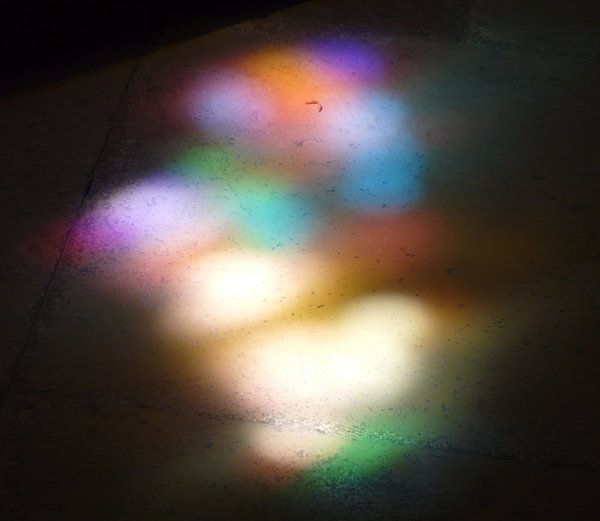
\includegraphics[height=6cm]{lichtspiel.jpg}}
\end{dispListing}
{\tcbset{reset}\tcbusetemp}

\end{docTcbKey}%v3 2023-1011 /v4 20231025
    % Typically, but not necessarily, a |tcolorbox| is put inside a separate paragraph and has some vertical space before and after it.
This behavior is controlled by the keys \refKey{/tcb/before} and \refKey{/tcb/after}.

通常情况下,但不一定,|tcolorbox| 放置在单独的段落中,并且在它前后有一些垂直空间。这种行为由键 \refKey{/tcb/before} 和 \refKey{/tcb/after} 控制。

% 通常情况下,但不是必须地,一个|tcolorbox|盒子被放置在单独的段落中,在它%之前和之后
% 的前后有一些垂直空间。%
% 这种行为是由\refKey{/tcb/before}和\refKey{/tcb/after}控制。

\begin{marker}
Before version 4.40, the default setting for \refKey{/tcb/before}
and \refKey{/tcb/after} was given by \refKey{/tcb/autoparskip}.
Starting with version 4.40, the default setting is given by
\refKey{/tcb/before skip balanced} and \refKey{/tcb/after skip balanced}.\par
Note that old documents may need adaptions of page breaks.\par
Alternatively, the old default setting can be restored by using

% 版本4.40之前,\refKey{/tcb/before}和\refKey{/tcb/after}的默认设置由\refKey{/tcb/autoparskip}控制。%
% 从4.40开始, 默认设置由\refKey{/tcb/before skip balanced}和\refKey{/tcb/after skip balanced}控制。\par
% 请注意,旧文档可能需要调整分页。\par
% 或者,可以使用以下命令恢复旧的默认设置

在版本4.40之前,\refKey{/tcb/before}和\refKey{/tcb/after}的默认设置由\refKey{/tcb/autoparskip}给出。从版本4.40开始,默认设置由\refKey{/tcb/before skip balanced}和\refKey{/tcb/after skip balanced}给出。请注意,旧文档可能需要调整分页。或者,可以通过使用以下方式恢复旧的默认设置:
\begin{dispListing}
\tcbsetforeverylayer{autoparskip}
\end{dispListing}
inside the document preamble.

在文档导言区中。
\end{marker}

\begin{docTcbKey}{before}{=\meta{code}}{no default, initially see \refKey{/tcb/before skip balanced}}
Sets the \meta{code} which is executed before the colored box.
It is not used for floating boxes.
Also, it is not used, if the box follows a heading immediately
and \refKey{/tcb/ignore nobreak} is set to \docValue{false}.

设置在盒子绘制之前执行的 \meta{code}。它不用于浮动框。如果盒子紧接着标题而来并且 \refKey{/tcb/ignore nobreak} 被设置为 \docValue{false},也不会使用。

% \meta{code}将在盒子绘制前执行。此项不用于浮动盒子。另外一个不生效的情况:如果盒子之前紧跟着标题且\refKey{/tcb/ignore nobreak}设为\docValue{false}.
\end{docTcbKey}

\begin{docTcbKey}{after}{=\meta{code}}{no default, initially see \refKey{/tcb/after skip balanced}}
Sets the \meta{code} which is executed after the colored box.
It is not used for floating boxes.

\meta{code}将在盒子绘制后执行。此项不用于浮动盒子。
\end{docTcbKey}


\begin{docTcbKey}{nobeforeafter}{}{style, no value}
Abbreviation for clearing the keys |before| and |after|. The colored box
is not put into a paragraph and there is no space before or after the box.

% 清除“之前”和“之后”密钥的缩写。彩色框不放入段落中,并且框前后没有空格。

清除|before|和|after|的简写形式。盒子没有放入段落中,盒子之前或之后没有空间。\footnote{译注:用上后,多个盒子就不会分行了}
\begin{exdispExample}{nobeforeafter}
\tcbset{myone/.style={colback=LightGreen,colframe=DarkGreen,
equal height group=nobefaf,width=\linewidth/4,nobeforeafter}}
\begin{tcolorbox}[myone,title=Box 1]Box 1\end{tcolorbox}%
\begin{tcolorbox}[myone,title=Box 2]Box 2\end{tcolorbox}%
\begin{tcolorbox}[myone,title=Box 3]Box 3\end{tcolorbox}%
\begin{tcolorbox}[myone,title=Box 4]Box 4\end{tcolorbox}
\end{exdispExample}
\end{docTcbKey}



\begin{docTcbKey}{force nobeforeafter}{}{style, no value}
Forces the setting of \refKey{/tcb/nobeforeafter} even if
\refKey{/tcb/before} and \refKey{/tcb/after} are set to other values
later. Do not use this option globally unless you \emph{really} know what you do.
Note that embedded boxes do not inherit this forced clearance.

强制设置\refKey{/tcb/nobeforeafter},甚至\refKey{/tcb/before}和\refKey{/tcb/after}是在这个选项设置之后又设置的。不要全局使用此选项,除非您\emph{真}的知道在做什么。注意,嵌套的盒子不会继承此项设置。
\end{docTcbKey}


%%\clearpage

\begin{docTcbKey}[][doc new={2020-09-25}]{before skip balanced}{=\meta{glue}}{no default, initially |0.5\textbackslash baselineskip plus 2pt|}
Inserts some vertical space before the colored box. This style sets \refKey{/tcb/before}.\par
在盒子之前插入一些垂直空间。该样式设置 \refKey{/tcb/before}。\par
% 在 tcolorbox 盒子之前,插入一些竖直的空白。此项也会设置 \refKey{/tcb/before}。\par
If the depth of the
preceeding \TeX\ box is between |0pt| and |0.3\baselineskip|,
the distance between the \emph{baseline} of the preceeding \TeX\ box and the tcolorbox
ist set to \meta{glue}$+$|0.3\baselineskip|.\par
如果前面的 \TeX\ 盒子的深度在 |0pt| 和 |0.3\baselineskip| 之间,前面的 \TeX\ 盒子的 \emph{基线} 与 tcolorbox 之间的距离设置为 \meta{glue}$+$|0.3\baselineskip|。\par
% 如果要处理的 \TeX\ 盒子的深度介于 |0pt| 到 |0.3\baselineskip|,
% \TeX\ 盒子的 \emph{基线} 到 tcolorbox 盒子间的空白高为 \meta{glue}$+$|0.3\baselineskip|.\par
If the depth is larger, the distance of the preceeding \TeX\ box and the tcolorbox
ist set to \meta{glue}.\par
如果深度更大,则前面的 \TeX\ 盒子与 tcolorbox 之间的距离设置为 \meta{glue}。\par
Alternatively, see \refKey{/tcb/before skip} which ignores the \emph{baseline}.

 或者,查看 \refKey{/tcb/before skip},该选项忽略了 \emph{基线}。
% 如果深度更大些, 则 \TeX\ 盒子和 tcolorbox 盒子间的空白设为 \meta{glue}.\par
% 也可以参阅 \refKey{/tcb/before skip},它忽略 \emph{baseline}.

\begin{exdispExample*}{before_skip_balanced}{sbs,lefthand ratio=0.6}
Some text.
\begin{tcolorbox}[before skip balanced=1cm,
colframe=red!50!white]
This is a \textbf{tcolorbox}.
\end{tcolorbox}
\end{exdispExample*}
\end{docTcbKey}


\begin{docTcbKey}[][doc new={2020-09-25}]{after skip balanced}{=\meta{glue}}{no default, initially |0.5\textbackslash baselineskip plus 2pt|}
Inserts some vertical space of the given \meta{glue} after the colored box.
This style sets \refKey{/tcb/after}.
Additionally, |\prevdepth| is set to |0.3\baselineskip|. The following
\TeX\ box may enlarge the space by further glue to adjust its \emph{baseline}.
Alternatively, see \refKey{/tcb/after skip} which ignores the \emph{baseline}.

插入指定的竖直空白到盒子后,高度为 \meta{glue}。%
此项会设置 \refKey{/tcb/after}。%
此外, |\prevdepth| 设为 |0.3\baselineskip|。下面的 \TeX\ 盒子可以通过弹性%进一步弹性来
扩大空间以调整其\emph{基线}。%
另见 \refKey{/tcb/after skip},它忽略 \emph{baseline}。

\begin{exdispExample*}{after_skip_balanced}{sbs,lefthand ratio=0.6}
\begin{tcolorbox}[after skip balanced=1cm,
colframe=red!50!white]
This is a \textbf{tcolorbox}.
\end{tcolorbox}
Some text.
\end{exdispExample*}
\end{docTcbKey}



\begin{docTcbKey}[][doc new={2020-09-25}]{beforeafter skip balanced}{=\meta{glue}}{no default, initially |0.5\textbackslash baselineskip plus 2pt|}
插入一些指定高度为 \meta{glue} 的垂直空间到盒子的前面和后面。
此项会同时设置 \refKey{/tcb/before skip balanced} 和 \refKey{/tcb/after skip balanced}。
todo tikzpicture
\begin{exdispExample*}{beforeafter_skip_balanced}{sbs,lefthand ratio=0.6}
\newtcolorbox{doubleline}[1][]{
beforeafter skip balanced=0pt,
height=1.8\baselineskip,
enlarge top by=.1\baselineskip,
enlarge bottom by=.1\baselineskip,
colframe=blue!20,colback=blue!5,
size=small,valign upper=center,#1 }

\noindent\begin{tikzpicture}
\path[use as bounding box] (0,0)
rectangle (0.1,0.1);
\foreach \y in {0,1,...,9}  {
\draw[very thin,red]
(-0.2,-\y*\baselineskip) --
(\linewidth+0.2cm,-\y*\baselineskip); }
\end{tikzpicture}
line 1\par
\begin{doubleline}  Abc  \end{doubleline}
\begin{doubleline}  Def  \end{doubleline}
line 2g\par
\begin{doubleline}  Ghi  \end{doubleline}
line 3\par
line 4 g
\end{exdispExample*}
\end{docTcbKey}



%%\clearpage

\begin{docTcbKey}[][doc new and updated={2020-09-25}{2015-03-16}]{before skip}{=\meta{glue}}{style, no default}
在盒子之前插入指定高度\meta{glue}的垂直空间。%
此项会设置 \refKey{/tcb/before}。%
同 \refKey{/tcb/before skip balanced} 相比, 这个 \meta{glue} upper 部分的边缘,并不是到基线位置。
\begin{exdispExample*}{before_skip}{sbs,lefthand ratio=0.6}
Some text.
\begin{tcolorbox}[before skip=1cm,
colframe=red!50!white]
This is a \textbf{tcolorbox}.
\end{tcolorbox}

Some text.
\begin{tcolorbox}[before skip=0cm,
colframe=red!50!white]
This is a \textbf{tcolorbox}.
\end{tcolorbox}
\end{exdispExample*}
\end{docTcbKey}

\begin{docTcbKey}[][doc new and updated={2020-09-25}{2017-02-01}]{after skip}{=\meta{glue}}{style, no default}
在盒子之后插入指定高度\meta{glue}的垂直空间。%
此项会设置 \refKey{/tcb/after}.
同 \refKey{/tcb/after skip balanced} 相比, %
这个 \meta{glue} 是相对于 lower 部分的边缘,并不是到基线位置。%\footnote{译注:后面有空想下英文原文是否有误?}
\begin{exdispExample*}{after_skip}{sbs,lefthand ratio=0.6}
\begin{tcolorbox}[after skip=1cm,
colframe=red!50!white]
This is a \textbf{tcolorbox}.
\end{tcolorbox}
Some text.
\end{exdispExample*}
\end{docTcbKey}

\begin{docTcbKey}[][doc new=2014-10-10]{beforeafter skip}{=\meta{glue}}{style, no default}
Inserts some vertical space of the given \meta{glue} before \emph{and} after the colored box.
This style sets \refKey{/tcb/before skip} and \refKey{/tcb/after skip}.

在盒子的前后插入指定高度\meta{glue}的垂直空间。%
此项会设置 \refKey{/tcb/before skip} 和 \refKey{/tcb/after skip}。


\begin{exdispExample*}{beforeafter_skip}{sbs,lefthand ratio=0.6}
\tcbset{beforeafter skip=0pt,
colframe=red!50!white}

text before
\begin{tcolorbox}
This is a \textbf{tcolorbox}.
\end{tcolorbox}
\begin{tcolorbox}
Second box.
\end{tcolorbox}
text after
\end{exdispExample*}
\end{docTcbKey}



%%\clearpage

\begin{docTcbKey}[][doc new=2014-11-07]{left skip}{=\meta{length}}{style, no default, initially |0mm|}
Inserts some horizontal space of the given \meta{length} before the colored box.
This style sets \refKey{/tcb/grow to left by} with the negated \meta{length},
i.e. the bounding box and box width are changed.

在盒子前插入给定 \meta{length} 的水平空间。
此项会设定 \refKey{/tcb/grow to left by} 为 \meta{length} 的相反数,
i.e. 边界框和盒子宽度已更改。
\begin{exdispExample*}{left_skip}{sbs,lefthand ratio=0.6}
\noindent\rule{\linewidth}{2pt}

\begin{tcolorbox}[left skip=1cm,
colframe=red!50!white]
This is a \textbf{tcolorbox}.
\end{tcolorbox}
\end{exdispExample*}
\end{docTcbKey}

\begin{docTcbKey}[][doc new=2014-11-07]{right skip}{=\meta{length}}{style, no default, initially |0mm|}
Inserts some horizontal space of the given \meta{length} after the colored box.
This style sets \refKey{/tcb/grow to right by} with the negated \meta{length},
i.e. the bounding box and box width are changed.

在盒子{\bf 后}插入给定 \meta{length} 的水平空间。%
此项会设定  \refKey{/tcb/grow to right by} 为 \meta{length} 的相反数,
i.e. 边界框和盒子宽度已更改。
\begin{exdispExample*}{right_skip}{sbs,lefthand ratio=0.6}
\noindent\rule{\linewidth}{2pt}

\begin{tcolorbox}[right skip=1cm,
colframe=red!50!white]
This is a \textbf{tcolorbox}.
\end{tcolorbox}
\end{exdispExample*}
\end{docTcbKey}



\begin{docTcbKey}[][doc new=2014-10-10]{leftright skip}{=\meta{length}}{style, no default}
Inserts some horizontal space of the given \meta{length} before \emph{and} after the colored box.
This style changes the bounding box and the box width.

在盒子前后插入给定长度为 \meta{length} 的水平空间。
此样式更改边界盒子和盒子宽度。

\begin{exdispExample*}{leftright_skip}{sbs,lefthand ratio=0.6}
\noindent\rule{\linewidth}{2pt}

\begin{tcolorbox}[leftright skip=1cm,
colframe=red!50!white]
This is a \textbf{tcolorbox}.
\end{tcolorbox}
\end{exdispExample*}
\end{docTcbKey}


%%\clearpage

\begin{docTcbKey}[][doc updated=2017-02-01]{parskip}{}{style, no value}
This options is considered to be superseded by
\refKey{/tcb/before skip balanced} and \refKey{/tcb/after skip balanced}
(see note on page~\pageref{subsec:surroundings}).\par
Sets the keys |before| and |after| to values which are
recommended, if the package |parskip| \emph{is} used and there is no better
idea for |before| and |after|. This is similar to:

此项有考虑使用 \refKey{/tcb/before skip balanced} 和 \refKey{/tcb/after skip balanced} 取代。
(见~\pageref{subsec:surroundings}页).\par
将 |before| 和 |after| 的值设置为推荐的值,如果{使用}了 |parskip| 包且 |before| 和 |after| 的值没有更好的主意。效果类似于:
\begin{dispListing}
\tcbset{parskip/.style={before={\par\pagebreak[0]\parindent=0pt},
                after={\par}}}
\end{dispListing}
\end{docTcbKey}

\begin{docTcbKey}[][doc updated=2017-02-01]{noparskip}{}{style, no value}
This options is considered to be superseded by
\refKey{/tcb/before skip balanced} and \refKey{/tcb/after skip balanced}
(see note on page~\pageref{subsec:surroundings}).\par
Sets the keys |before| and |after| to values which are
recommended, if the package |parskip| is \emph{not} used and there is no better
idea for |before| and |after|. This is similar to:

此项有考虑使用 \refKey{/tcb/before skip balanced} 和 \refKey{/tcb/after skip balanced} 取代。
(见~\pageref{subsec:surroundings}页).\par
将 |before| 和 |after| 的值设置为推荐的值,如果{使用}了 |parskip| 包且 |before| 和 |after| 的值没有更好的主意。效果类似于:
\begin{dispListing}
\tcbset{noparskip/.style={before={\par\pagebreak[0]\smallskip\parindent=0pt},
                    after={\par\smallskip}}}
\end{dispListing}
\end{docTcbKey}



\begin{docTcbKey}{autoparskip}{}{style, no value}
This options is considered to be superseded by
\refKey{/tcb/before skip balanced} and \refKey{/tcb/after skip balanced}
(see note on page~\pageref{subsec:surroundings}).\par
Tries to detect the usage of the package |parskip| and sets
the keys |before| and |after| accordingly. Actually, the following is done:

这项可以考虑改用 \refKey{/tcb/before skip balanced} 和 \refKey{/tcb/after skip balanced} 替换(另见~\pageref{subsec:surroundings}~页)。\par
尝试检测 |parskip| 的使用情况, 并相应的设置 |before| 和 |after|。 实际上,完成了以下操作:

\begin{itemize}
\item 
If the length of |\parskip| is greater than |0pt| at the beginning of the document,
\refKey{/tcb/parskip} is executed. Here, the usage of package |parskip| is \emph{assumed}.

todo
如果在文档的开头 |\parskip| 的值大于|0pt|,%
\refKey{/tcb/parskip} 将会执行。 这里, 假定 |parskip| 引入\footnote{Here, the usage of package |parskip| is \emph{assumed}}。

\item 
Otherwise, if the length of |\parskip| is not greater than |0pt| at the beginning of the document,
\refKey{/tcb/noparskip} is executed. Here, the absence of package |parskip| is \emph{assumed}.
另外,如果在文档的开头 |\parskip| 的值不大于|0pt|,%
\refKey{/tcb/noparskip} 将会执行。 这里, 假定 |parskip| 没有使用\footnote{Here, the absence of package |parskip| is \emph{assumed}}。
\end{itemize}
\end{docTcbKey}




%%\clearpage

\begin{docTcbKey}{baseline}{=\meta{length}}{no default, initially |0pt|}
Used to set the |\pgfsetbaseline| value of the resulting |tcolorbox|.
设置结果盒子的%,同其他 \TeX\ 对象对齐用的
基线的值(|\pgfsetbaseline|)。

\begin{exdispExample}{baseline}
\tcbset{colframe=red!50!white,width=4cm,nobeforeafter}
Some text\dotfill
\begin{tcolorbox}[baseline=3mm]
第一行
\end{tcolorbox}
\begin{tcolorbox}[baseline=3mm]
第一行\\第二行
\end{tcolorbox}
\begin{tcolorbox}[baseline=4mm]
第一行\\第二行\\第三行
\end{tcolorbox}
\end{exdispExample}
\end{docTcbKey}




\begin{docTcbKey}[][doc new=2014-10-10]{box align}{=\meta{alignment}}{style, no default, initially |bottom|}
Used to set the \refKey{/tcb/baseline} value of the resulting |tcolorbox|.
Feasible values for \meta{alignment} are:

Used to set the \refKey{/tcb/baseline} value of the resulting |tcolorbox|.
Feasible values for \meta{alignment} are:  
\begin{itemize}
\item\docValue{bottom}: %alignment with the box bottom,
与盒子底部对齐,
\item\docValue{top}: %alignment with the box top,
与盒子顶部对齐,
\item\docValue{center}: %alignment with the box center,
与盒子中心对齐,
\item\docValue{base}: 
alignment with the box content base. This option
is not applicable for a \refEnv{tcolorbox} but for a \refCom{tcbox} only.
It is an alias for \refKey{/tcb/tcbox raise base}.
与盒子内容的基线对齐。此项不在 \refEnv{tcolorbox} 使用,仅在 \refCom{tcbox} 生效。
这是 \refKey{/tcb/tcbox raise base} 的别名。
\end{itemize}

\begin{exdispExample}{box_align_1}
\tcbset{colframe=red!50!white,width=4cm,nobeforeafter}
Some text\dotfill
\begin{tcolorbox}[box align=bottom]
bottom
\end{tcolorbox}
\begin{tcolorbox}[box align=bottom]
bottom\\bottom
\end{tcolorbox}
\begin{tcolorbox}
第一行\\第二行\\第三行
\end{tcolorbox}
\end{exdispExample}

\begin{exdispExample}{box_align_2}
\tcbset{colframe=red!50!white,width=4cm,nobeforeafter}
Some text\dotfill
\begin{tcolorbox}[box align=top]
top
\end{tcolorbox}
\begin{tcolorbox}[box align=top]
top\\top
\end{tcolorbox}
\begin{tcolorbox}
第一行\\第二行\\第三行
\end{tcolorbox}
\end{exdispExample}

\begin{exdispExample}{box_align_3}
\tcbset{colframe=red!50!white,width=4cm,nobeforeafter}
Some text\dotfill
\begin{tcolorbox}[box align=center]
center
\end{tcolorbox}
\begin{tcolorbox}[box align=center]
center\\center
\end{tcolorbox}
\begin{tcolorbox}
第一行\\第二行\\第三行
\end{tcolorbox}
\end{exdispExample}

\begin{exdispExample}{box_align_4}
\tcbset{colframe=red!50!white,nobeforeafter}
Some text\dotfill
\tcbox[nobeforeafter,box align=base]{base}
\tcbox[nobeforeafter,box align=base,size=fbox]{base}
\tcbox[nobeforeafter]{未设置}
\end{exdispExample}
\end{docTcbKey}





\begin{docTcbKey}[][doc new=2014-12-11]{ignore nobreak}{\colOpt{=true\textbar false}}{default |true|, initially |false|}
After a heading, \LaTeX\ tries to avoid a break by setting a |nobreak| boolean value.
Starting from version |3.33|, the \refKey{/tcb/before} respectively \refKey{/tcb/before skip}
settings are not used after a heading if \refKey{/tcb/ignore nobreak} is
set to \docValue{false}. For an unbreakable box, \refKey{/tcb/before nobreak} is used instead.
Further, a \refKey{/tcb/breakable} box will also try to
avoid a break between a heading and a directly following first part of a
break sequence.

在标题之后, 通过设置 |nobreak| ,\LaTeX\ 会尝试避免分页。
从版本 |3.33| 开始, 如果 \refKey{/tcb/ignore nobreak} 设置为 \docValue{false}, 那么 \refKey{/tcb/before} 和 \refKey{/tcb/before skip}
的设置在标题之后将不生效。%
对于一个不可分的盒子, 将使用 \refKey{/tcb/before nobreak} 替代使用。
将来, 一个设置了 \refKey{/tcb/breakable} 的盒子,将会尝试避免在标题和紧随其后的中断序列的第一部分之间中断。

Set \refKey{/tcb/ignore nobreak} to \docValue{true}, if |nobreak| should be
ignored as prior to version |3.33|. Also, such a setting may be used locally to
enforce the \refKey{/tcb/before} setting.
在版本 |3.33|,如果需要保留这个忽略 |nobreak| 的效果,将 \refKey{/tcb/ignore nobreak} 设置为 \docValue{true}。 此外,这样的设置可以在 locally 使用以强制设置 \refKey{/tcb/before} 。
\end{docTcbKey}

\begin{docTcbKey}[][doc new=2014-12-16]{before nobreak}{=\meta{code}}{no default, initially \cs{noindent}}
Sets the \meta{code} which is executed before the colored box if it
is unbreakable, if \refKey{/tcb/ignore nobreak} is not set, and if
the box follows a heading.

如果是不可以分的,设置 \meta{code} 在盒子之前执行, 如果没有设置 \refKey{/tcb/ignore nobreak} , 或如果盒子是跟随在标题之后。
\end{docTcbKey}



\begin{docTcbKey}[][doc new=2017-02-23]{parfillskip restore}{\colOpt{=true\textbar false}}{default |true|, initially |true|}
If this option is set to be |true|, the minimum value of |\parfillskip| is
tested at specific spots, if it is greater than |0pt|.
If so, |\parfillskip| is restored to |\@flushglue| which happens to be
the default value.

如果此项设置为 |true|, 则在特定点测试 |\parfillskip| 的最小值, 如果它大于 |0pt|.
如果是这样,|\parfillskip| 恢复到 |\@flushglue|, 这恰好是默认值。

These tests are executed for
这些判断将会在以下位置执行:
\refKey{/tcb/parskip},
\refKey{/tcb/noparskip},
\refKey{/tcb/after skip},
\refKey{/tcb/breakable}, and
\refEnv{tcbraster}.

This option was created to automatically
avoid overfull box warnings with |\parfillskip| changing packages.

创建此选项是为了自动避免 |\parfillskip| 改变包裹带来的 |overfull box| 警告 。
\end{docTcbKey}%可以再看看,例子修改,分成几个文件  %v3 2023-1011 /v4 20231025
    % 
Normally, every |tcolorbox| has a bounding box which fits exactly to the
dimensions of the outer frame. Therefore, \LaTeX\ reserves exactly the space
needed for the box.
This behavior can be changed by enlarging (or shrinking) the bounding box.
If the bounding box is enlarged, the |tcolorbox| will get some clearance
around it. If the bounding box is shrunk, i.\,e.\ enlarged with negative
values, the |tcolorbox| will overlap to other parts of the page.
For example, the |tcolorbox| could be stretched into the page margin.

通常,每个 |tcolorbox| 都有一个边界框,它恰好适合外部框架的尺寸。因此,\LaTeX\ 精确地保留了盒子所需的空间。 可以通过放大(或缩小)边界框来改变这种行为。 如果边界框被放大,|tcolorbox| 将在其周围获得一些间隙。 如果边界框被缩小,即用负值放大,|tcolorbox| 将与页面的其他部分重叠。 例如,|tcolorbox| 可以延伸到页面边缘。

% 通常,每个 |tcolorbox| 盒子有一个与其外框严丝合缝的边界盒子。%
% 因此,\LaTeX\ 保留了盒子所需的空间。%
% 可以通过扩大(或缩小)边界盒子来更改此空间。%
% 如果边界盒子被放大, 那么 |tcolorbox| 的周围将多出一些空间。 如果边界框缩小, i.\,e.\ 扩大一个负值, |tcolorbox| 将重叠到页面的其他部分。%
% 例如,|tcolorbox| 可能会突到页边距去。

\begin{marker}
The following examples use \refKey{/tcb/show bounding box} to display the actual bounding box. For this, the library \mylib{skins} has to be included and \refKey{/tcb/enhanced} has to be set.

以下示例使用\refKey{/tcb/show bounding box}来显示实际边界框。为此,必须包含库\mylib{skins}并设置\refKey{/tcb/enhanced}。
% 以下示例使用 \refKey{/tcb/show bounding box} 来显示实际的边界框。为此,必须包含库 \mylib{skins} 并且必须设置 \refKey{/tcb/enhanced}。
\end{marker}



\subsubsection{Shifting Bounding Box Borders\\移动边界盒子的边框}

\begin{docTcbKey}{enlarge top initially by}{=\meta{length}}{no default, initially |0mm|}
Enlarges the bounding box distance to the top of the box by \meta{length}.
If the box is \emph{breakable}, only the first box of the break sequence
gets enlarged. \refKey{/tcb/enlarge top by} overwrites this key.

将边框顶部的边界框距离增加\meta{length}。如果该盒子是\emph{可分页的},则仅对分页序列的第一个框进行扩展。 \refKey{/tcb/enlarge top by} 覆盖此键。 

% 扩大边界盒子同 |tcolorbox| 盒子的顶部的距离 \meta{length}。
% 如果 |tcolorbox| 盒子是\emph{可分的}, 只有中断序列的第一个盒子的扩大会生效。 
\refKey{/tcb/enlarge top by} 会覆盖这个设置。
\begin{exdispExample}{enlarge_top_initially_by}
\tcbset{colframe=blue!75!black,colback=white}

\begin{tcolorbox}[enlarge top initially by=-5mm]
This is a \textbf{tcolorbox}.
\end{tcolorbox}
\begin{tcolorbox}[enlarge top initially by=5mm,enhanced,show bounding box]
This is a \textbf{tcolorbox}.
\end{tcolorbox}
\end{exdispExample}
\end{docTcbKey}

\begin{tcolorbox}[nobeforeafter]
\textbf{tcolorbox} a.
\end{tcolorbox}
\begin{tcolorbox}[nobeforeafter]
\textbf{tcolorbox} b.
\end{tcolorbox}




\begin{docTcbKey}{enlarge bottom finally by}{=\meta{length}}{no default, initially |0mm|}
Enlarges the bounding box distance to the bottom of the box by \meta{length}.
If the box is \emph{breakable}, only the last box of the break sequence
gets enlarged. \refKey{/tcb/enlarge bottom by} overwrites this key.

通过\meta{length}来增加盒子底部的边界距离。如果该盒子是\emph{可分割}的,那么只有分割序列的最后一个盒子会被放大。 \refKey{/tcb/enlarge bottom by} 会覆盖此关键字。

% 扩大边界盒子同 |tcolorbox| 盒子的底部的距离 \meta{length}。%
% 如果盒子是 \emph{可中断的}, 只有中断序列的最后一部分得到扩大。
% \refKey{/tcb/enlarge bottom by} 会覆盖这个设置。
\begin{exdispExample}{enlarge_bottom_finally_by}
\tcbset{colframe=blue!75!black,colback=white}

\begin{tcolorbox}[enlarge bottom finally by=5mm]
This is a \textbf{tcolorbox}.
\end{tcolorbox}
\begin{tcolorbox}[enlarge bottom finally by=-5mm,enhanced,show bounding box]
This is a \textbf{tcolorbox}.
\end{tcolorbox}
\end{exdispExample}
\end{docTcbKey}

%%\clearpage




\begin{docTcbKey}{enlarge top at break by}{=\meta{length}}{no default, initially \texttt{0mm}}
Enlarges the bounding box distance to the top of the box by \meta{length},
\emph{if} the box is \refKey{/tcb/breakable}.
In this case, it is applied to \emph{middle} and \emph{last} parts in a
break sequence.
\refKey{/tcb/enlarge top by} overwrites this key.

\emph{如果}盒子是 \refKey{/tcb/breakable}的,扩大边界盒子同 |tcolorbox| 盒子的顶部的距离 \meta{length}。这种情况下, 它在 \emph{中间}和\emph{最后}的中断序列部分生效。 \refKey{/tcb/enlarge top by} 会覆盖此项设置。
\end{docTcbKey}


\begin{docTcbKey}{enlarge bottom at break by}{=\meta{length}}{no default, initially \texttt{0mm}}
Enlarges the bounding box distance to the bottom of the box by \meta{length},
\emph{if} the box is \refKey{/tcb/breakable}.
In this case, it is applied to \emph{first} and \emph{middle} parts in a
break sequence. \refKey{/tcb/enlarge bottom by} overwrites this key.

\emph{如果}盒子是 \refKey{/tcb/breakable}的,扩大边界盒子同 |tcolorbox| 盒子的底部的距离 \meta{length}。
这种情况下, 它在 \emph{首个}和\emph{中间}的中断序列部分生效。
\refKey{/tcb/enlarge bottom by} 会覆盖此项设置。
\end{docTcbKey}




\begin{docTcbKey}{enlarge top by}{=\meta{length}}{no default, initially |0mm|}

Enlarges the bounding box distance to the top of the box by \meta{length}.
\refKey{/tcb/enlarge top initially by} and
\refKey{/tcb/enlarge top at break by} are set to \meta{length}.

扩大边界盒子同 |tcolorbox| 盒子的{\bf 顶}部的距离 \meta{length}。
\refKey{/tcb/enlarge top initially by} 和
\refKey{/tcb/enlarge top at break by} 也会被设置为 \meta{length}。
\end{docTcbKey}


\begin{docTcbKey}{enlarge bottom by}{=\meta{length}}{no default, initially |0mm|}
Enlarges the bounding box distance to the bottom of the box by \meta{length}.
\refKey{/tcb/enlarge bottom finally by} and
\refKey{/tcb/enlarge bottom at break by} are set to \meta{length}.

扩大边界盒子同 |tcolorbox| 盒子的{\bf 底}部的距离 \meta{length}。
\refKey{/tcb/enlarge bottom finally by} 和
\refKey{/tcb/enlarge bottom at break by} 也会被设为 \meta{length}.
\end{docTcbKey}



\begin{docTcbKey}{enlarge left by}{=\meta{length}}{no default, initially |0mm|}
Enlarges the bounding box distance to the left side of the box by \meta{length}.

扩大边界盒子同 |tcolorbox| 盒子的{\bf 左侧}的距离 \meta{length}。
\begin{exdispExample}[safety=2cm]{enlarge_left_by}
\tcbset{colframe=blue!75!black,colback=white}

\begin{tcolorbox}[enlarge left by=2cm,width=5cm,enhanced,show bounding box]
This is a \textbf{tcolorbox}.
\end{tcolorbox}
\begin{tcolorbox}[enlarge left by=-2cm,width=\linewidth+2cm]
This is a \textbf{tcolorbox}.
\end{tcolorbox}
\end{exdispExample}
\end{docTcbKey}

\begin{docTcbKey}{enlarge right by}{=\meta{length}}{no default, initially |0mm|}
Enlarges the bounding box distance to the right side of the box by \meta{length}.

扩大边界盒子同 |tcolorbox| 盒子的{\bf 右侧}的距离 \meta{length}。
\begin{exdispExample}[safety=2cm]{enlarge_right_by}
\tcbset{colframe=blue!75!black,colback=white}

\begin{tcolorbox}[enlarge right by=-2cm,width=\linewidth+2cm,
enhanced,show bounding box]
\textbf{tcolorbox}缩小了同右侧的距离到负数,就突出到右边了.
\end{tcolorbox}
\begin{tcolorbox}[enlarge right by=2cm,width=\linewidth-2cm]
This is a \textbf{tcolorbox}.
\end{tcolorbox}
\end{exdispExample}
\end{docTcbKey}




%%\clearpage
\begin{docTcbKey}{enlarge by}{=\meta{length}}{no default, initially |0mm|}
Enlarges the bounding box distance to all sides of the box by \meta{length}.

扩大边界盒子同 |tcolorbox| 盒子的{\bf 四侧}的距离 \meta{length}。
\begin{exdispExample}{enlarge_by}
\tcbset{colframe=blue!75!black,colback=white,width=5cm,nobeforeafter}

\begin{tcolorbox}
This is a \textbf{tcolorbox}.
\end{tcolorbox}
\begin{tcolorbox}[enlarge by=5mm,enhanced,show bounding box]
This is a \textbf{tcolorbox}.
\end{tcolorbox}
\end{exdispExample}
\end{docTcbKey}





\begin{docTcbKey}{grow to left by}{=\meta{length}}{no default, initially |0mm|}
Enlarges the current box width by \meta{length} and
enlarges (shrinks) the bounding box distance to the left side of the box by
$-$\meta{length}. Also see \refKey{/tcb/left skip}.

扩大当前盒子的宽度\meta{length},并扩大边界盒子到左侧的距离为
$-$\meta{length}。\footnote{突出到左侧了} 另见 \refKey{/tcb/left skip}。
\begin{exdispExample}[safety=2cm]{grow_to_left_by}
\tcbset{colframe=blue!75!black,colback=white}

\begin{tcolorbox}[width=5cm,grow to left by=2cm,enhanced,show bounding box]
This is a \textbf{tcolorbox} with a width of 7cm.
\end{tcolorbox}
\end{exdispExample}
\end{docTcbKey}

\begin{docTcbKey}{grow to right by}{=\meta{length}}{no default, initially |0mm|}
Enlarges the current box width by \meta{length} and
enlarges (shrinks) the bounding box distance to the right side of the box by
$-$\meta{length}. Also see \refKey{/tcb/right skip}.

扩大当前盒子的宽度\meta{length},并扩大边界盒子到右侧的距离为
$-$\meta{length}。\footnote{突出到右侧了} 另见 \refKey{/tcb/right skip}。
\begin{exdispExample}[safety=2cm]{grow_to_right_by}
\tcbset{colframe=blue!75!black,colback=white}

\begin{tcolorbox}[grow to right by=2cm,enhanced,show bounding box]
This is a \textbf{tcolorbox}.
\end{tcolorbox}

\bigskip

\begin{tcolorbox}[grow to right by=2cm,grow to left by=1cm,
enhanced,show bounding box]
This is a \textbf{tcolorbox}.
\end{tcolorbox}
\end{exdispExample}
\end{docTcbKey}

%%\clearpage


\begin{docTcbKey}[][doc new=2018-03-22]{grow sidewards by}{=\meta{length}}{no default, initially |0mm|}
Shortcut for setting \refKey{/tcb/grow to left by} and \refKey{/tcb/grow to right by}
to \meta{length}. Also see \refKey{/tcb/oversize} and \refKey{/tcb/spread sidewards}.

同时设置 \refKey{/tcb/grow to left by} 和 \refKey{/tcb/grow to right by} 到\meta{length} 的简写形式。另见 \refKey{/tcb/oversize} 和 \refKey{/tcb/spread sidewards}.
\begin{exdispExample}[safety=2cm]{grow_sidewards_by}
\tcbset{colframe=blue!75!black,colback=white}

\begin{tcolorbox}[grow sidewards by=2cm,enhanced,show bounding box]
This is a \textbf{tcolorbox}.
\end{tcolorbox}
\end{exdispExample}
\end{docTcbKey}




\subsubsection{Box Alignment\\盒子的对齐}

\begin{docTcbKey}[][doc new=2015-11-20]{flush left}{}{style, no value}
Enlarges the bounding box to the right side to fill the line completely.

左对齐效果,扩大边界盒子完全填充到右侧。
\begin{exdispExample}{flush_left}
\tcbset{colframe=blue!75!black,colback=white}

\begin{tcolorbox}[flush left,width=5cm,enhanced,show bounding box]
This is a \textbf{tcolorbox}.
\end{tcolorbox}
\end{exdispExample}
\end{docTcbKey}


\begin{docTcbKey}[][doc new=2015-11-20]{flush right}{}{style, no value}
Enlarges the bounding box to the left side to fill the line completely.

右对齐效果,扩大边界盒子完全填充到左侧。
\begin{exdispExample}{flush_right}
\tcbset{colframe=blue!75!black,colback=white}

\begin{tcolorbox}[flush right,width=5cm,enhanced,show bounding box]
This is a \textbf{tcolorbox}.
\end{tcolorbox}
\end{exdispExample}
\end{docTcbKey}


\begin{docTcbKey}[][doc new=2015-11-20]{center}{}{style, no value}
Enlarges the bounding box equally to both sides to fill the line completely.

居中对齐效果,扩大边界盒子完全填充到两侧。
\begin{exdispExample}{center}
\tcbset{colframe=blue!75!black,colback=white}

\begin{tcolorbox}[center,width=5cm,enhanced,show bounding box]
This is a \textbf{tcolorbox}.
\end{tcolorbox}
\end{exdispExample}
\end{docTcbKey}




%%\clearpage

\subsubsection{Toggle Enlargements}

\begin{docTcbKey}[][doc updated=2015-11-13]{toggle enlargement}{=\meta{toggle preset}}{默认 |evenpage|(偶), initially |none|}
According to the \meta{toggle preset}, the left and the right enlargements of
the bounding box are switched or not. Feasible values are:

依据 \meta{toggle preset} 的值, 对边界盒子的左边和右边的增加空间的设置进行交换或不交换。可设的值有:
\begin{itemize}
\item\docValue{none}: %no switching.
不切换。
\item\docValue{forced}: %the values of the left and right enlargement are switched.
强制将边界盒子的左边和右边的增加空间的设置进行交换。
\item\docValue{evenpage}: 
if the page is an even page, the values of the left and    right enlargement are switched. This value also sets    \refKey{/tcb/check odd page} to |true|.

如果当前页是偶数页, 将边界盒子的左边和右边的增加空间的设置进行交换。这项值也会将  \refKey{/tcb/check odd page} 设置为 |true|.
\end{itemize}
\begin{marker}
See \refKey{/tcb/toggle left and right} to toggle geometry settings.
见 \refKey{/tcb/toggle left and right} 来切换几何设置。
\end{marker}

\begin{dispExample}
\tcbset{colframe=blue!75!black,colback=white,
grow to left by=20mm,%突出左侧
grow to right by=-5mm%右侧凹着
}

\begin{tcolorbox}[toggle enlargement=none
,enhanced,show bounding box]
设置为 |toggle enlargement=none|,不切换
\end{tcolorbox}
\begin{tcolorbox}[toggle enlargement=forced]
设置为 |toggle enlargement=forced|,强制切换
\end{tcolorbox}
\begin{tcolorbox}[toggle enlargement=evenpage]
设置为 |toggle enlargement=evenpage|,偶数页才切换。当前页是 \tcbifoddpage{奇}{偶} 数页。因此, 左边的增加空间的设置 \tcbifoddpage{不会}{会}切换。
\end{tcolorbox}
\end{dispExample}

\begin{dispListing}
\begin{tcolorbox}[colframe=red!60!black,colback=red!15!white,
fonttitle=\bfseries,title=Floating box from \texttt{toggle enlargement},
width=\textwidth
,grow to right by=2cm%突出到右边
,toggle enlargement%默认是偶数页
,float=t]
当前页是\tcbifoddpage{奇}{偶}数页。%
因此, 左边的增加空间的设置 \tcbifoddpage{不会}{会}切换。%
这个盒子,在奇数页是突出到右边,在偶数页是突出到左边。%
本文档是one-sided文档 -- 这项特性只在two-sided%
\footnote{译注:即双面打印,%
奇数和偶数页的文档内容的左右边距是不同的,以用于装订。}%
文档中生效。
\end{tcolorbox}
\end{dispListing}
\tcbusetemp
\end{docTcbKey}





%%\clearpage

\subsubsection{Spread Box to Page Borders\\盒子扩张到页面边缘}

\begin{marker} 
The following border options are \emph{not} applicable to nested boxes, boxes insides tables, etc.
For boxes inside lists, the options \emph{may} work, but not necessarily.
Also, boxes should be set with |\noindent| and full width.

以下的 border 选项对嵌套的盒子, 在表格中的盒子\emph{不}起作用, etc.
对于列表中的盒子,这些选项\emph{可以}工作, 但没必要。
另外,盒子需要设置 |\noindent| 来达到全宽。
\end{marker}

\begin{docTcbKey}[][doc new=2017-02-13]{spread inwards}{\colOpt{=\meta{length}}}{default |0pt|, initially unset}
Enlarges the current box width to match the inner page border (left-handed side for one-sided
documents). If the optional \meta{length} is greater than |0pt|, the box
grows over the border, if \meta{length} is lower than |0pt|, there is a
margin between box and page border.
\refKey{/tcb/toggle enlargement} is set automatically.

扩张当前盒子的宽度到书本的内页边缘(对单面文档是在左侧).如果选项的值\meta{length}是大于 |0pt|, 那么盒子将穿过页面的边缘, 如果\meta{length}是小于|0pt|,那么在盒子和页面边缘就有一段面边空白。会自动设置 \refKey{/tcb/toggle enlargement} 。
\begin{dispListing}
\begin{tcolorbox}[enhanced,spread inwards,
colframe=blue!75!black,colback=white,show bounding box]
扩张当前盒子的宽度到书本的内页边缘 (对单面文档是在左侧).(|spread inwards|)
\end{tcolorbox}

\begin{tcolorbox}[enhanced,spread inwards=2em,
colframe=blue!75!black,colback=white,show bounding box]
前面的内容穿过边缘了(|spread inwards=2em,|)。
\end{tcolorbox}

\begin{tcolorbox}[enhanced,spread inwards=-2em,
colframe=blue!75!black,colback=white,show bounding box]
在盒子和页面边缘就有一段面边空白。(|spread inwards=-2em,|)。
\end{tcolorbox}
\end{dispListing}
{\tcbusetemp}
\end{docTcbKey}



\begin{docTcbKey}[][doc new=2017-02-13]{spread outwards}{\colOpt{=\meta{length}}}{default |0pt|, initially unset}
Enlarges the current box width to match the outer page border (right-handed side for one-sided
documents). If the optional \meta{length} is greater than |0pt|, the box
grows over the border, if \meta{length} is lower than |0pt|, there is a
margin between box and page border.
\refKey{/tcb/toggle enlargement} is set automatically.

扩张当前盒子的宽度到书本的内页边缘(对单面文档是在右侧)。如果选项的值\meta{length}是大于 |0pt|, 那么盒子将穿过页面的边缘, 如果\meta{length}是小于|0pt|,那么在盒子和页面边缘就有一段空白。会自动设置 \refKey{/tcb/toggle enlargement} 。

\begin{dispListing}
\begin{tcolorbox}[enhanced,spread outwards,
colframe=blue!75!black,colback=white,show bounding box]
This is a \textbf{tcolorbox}.
\end{tcolorbox}
\end{dispListing}
{\tcbusetemp}
\end{docTcbKey}


\begin{docTcbKey}[][doc new=2017-02-13]{move upwards}{\colOpt{=\meta{length}}}{default |0pt|, initially unset}
Starts a new page with the box at the very top page border.
If the optional \meta{length} is greater than |0pt|, the box
moves over the border, if \meta{length} is lower than |0pt|, there is a
margin between box and page border.

新起一页,将盒子放在新页面的最顶部。%
如果选项的值\meta{length}是大于 |0pt|, 那么盒子将穿过页面的边缘, 如果\meta{length}是小于|0pt|,那么在盒子和页面边缘就有一段空白。
\end{docTcbKey}


\begin{docTcbKey}[][doc new=2017-02-13]{move upwards*}{\colOpt{=\meta{length}}}{default |0pt|, initially unset}
同\refKey{/tcb/move upwards}一样,但少了新起一页的操作。
\end{docTcbKey}




\begin{docTcbKey}[][doc new=2017-02-13]{fill downwards}{\colOpt{=\meta{length}}}{default |0pt|, initially unset}
Enlarges the height of the box until the very bottom page border.
The library \mylib{breakable} has to be loaded, and
\refKey{/tcb/height fill} is set automatically.
If the optional \meta{length} is greater than |0pt|, the box
moves over the border, if \meta{length} is lower than |0pt|, there is a
margin between box and page border.

扩张当前盒子的宽度到书本的底部边缘。%
需要加载 \mylib{breakable} 库, 且会自动设置\refKey{/tcb/height fill} 。%
如果选项的值\meta{length}是大于 |0pt|, 那么盒子将穿过页面的边缘, 如果\meta{length}是小于|0pt|,那么在盒子和页面边缘就有一段空白。
\begin{dispListing}
\begin{tcolorbox}[enhanced,fill downwards,
colframe=blue!75!black,colback=white,show bounding box]
扩张当前盒子的宽度到书本的底部边缘。
\end{tcolorbox}
\end{dispListing}
{\tcbusetemp}
\end{docTcbKey}


\begin{tcolorbox}[enhanced,spread upwards,sharp corners=north,height=3cm,
colframe=blue!75!black,interior style={top color=blue!50,bottom color=white}]
这是\enquote{spread upwards}的例子。 
\end{tcolorbox}
\begin{docTcbKey}[][doc new=2017-02-13]{spread upwards}{\colOpt{=\meta{length}}}{default |0pt|, initially unset}
组合,同时将\meta{length}设到
\refKey{/tcb/move upwards}, \refKey{/tcb/spread inwards}, 和 \refKey{/tcb/spread outwards}.
\begin{dispListing}
\begin{tcolorbox}[enhanced,spread upwards,sharp corners=north,height=3cm,
colframe=blue!75!black,interior style={top color=blue!50,bottom color=white}]
这是 \enquote{spread upwards} 的例子。
\end{tcolorbox}
\end{dispListing}
\end{docTcbKey}


\begin{docTcbKey}[][doc new=2017-02-13]{spread upwards*}{\colOpt{=\meta{length}}}{default |0pt|, initially unset}
同\refKey{/tcb/move upwards}一样,但不会新起一页。
\end{docTcbKey}




\begin{docTcbKey}[][doc new=2017-02-13]{spread sidewards}{\colOpt{=\meta{length}}}{default |0pt|, initially unset}
Combination of \refKey{/tcb/spread inwards} and \refKey{/tcb/spread outwards}.
The optional \meta{length} is used for all these keys.
Also see \refKey{/tcb/oversize} and \refKey{/tcb/grow sidewards by}.

\meta{length}被同时设置到 \refKey{/tcb/spread inwards} 和 \refKey{/tcb/spread outwards}。另见 \refKey{/tcb/oversize} 和 \refKey{/tcb/grow sidewards by}.
\begin{dispListing}
\begin{tcolorbox}[enhanced,spread sidewards,
colframe=blue!75!black,colback=white,show bounding box]
向左右两侧突出了。
\end{tcolorbox}
\end{dispListing}
{\tcbusetemp}
\end{docTcbKey}


\begin{docTcbKey}[][doc new=2017-02-13]{spread}{\colOpt{=\meta{length}}}{default |0pt|, initially unset}
Combination of
\refKey{/tcb/move upwards}, \refKey{/tcb/fill downwards}, \refKey{/tcb/spread inwards},
and \refKey{/tcb/spread outwards}.
Such, the box fills the whole page.
The optional \meta{length} is used for all these keys.

组合了 \refKey{/tcb/move upwards}, \refKey{/tcb/fill downwards}, \refKey{/tcb/spread inwards},和 \refKey{/tcb/spread outwards}。
这样,盒子就填满了整个页面。
\meta{length} 被同时设置到这些选项。
\end{docTcbKey}




\begin{docTcbKey}[][doc new=2017-02-13]{spread downwards}{\colOpt{=\meta{length}}}{default |0pt|, initially unset}
Combination of
\refKey{/tcb/fill downwards}, \refKey{/tcb/spread inwards}, and \refKey{/tcb/spread outwards}.
The optional \meta{length} is used for all these keys.

组合使用 \refKey{/tcb/fill downwards}, \refKey{/tcb/spread inwards}, 和 \refKey{/tcb/spread outwards}.
\meta{length} 被同时设置到这些选项。
\begin{dispListing}
\begin{tcolorbox}[enhanced,spread downwards,sharp corners=south,
colframe=red!75!black,interior style={top color=white,bottom color=red!50}]
This is an example for \enquote{spread downwards}.
\end{tcolorbox}
\end{dispListing}
\end{docTcbKey}
\begin{tcolorbox}[enhanced,spread downwards,sharp corners=south,
colframe=red!75!black,interior style={top color=white,bottom color=red!50}]
This is an example for \enquote{spread downwards}.
\end{tcolorbox}






%%\clearpage

\subsubsection{Box Extrusion\\挤压盒子}

\begin{marker}
The following keys should not be used with breakable boxes or boxes with a
lower part.

以下选项不应在可分盒子或带有lower部分的盒子内使用。
\end{marker}

\begin{docTcbKey}{shrink tight}{}{style, no value, initially unset}
The total colored box is shrunk to the dimensions of the upper
part. There should be no lower part and no title.
This style sets the \refKey{/tcb/boxsep} to |0pt| and other geometry keys
to fitting values. This option is likely to be used with the following
extrusion keys.

整个盒子缩小到upper部分的尺寸。不应有lower部分和标题。
此样式会将 \refKey{/tcb/boxsep} 设置为 |0pt|,以及一些其他几何设置。此选项可能与以下挤压键一起使用。
\begin{exdispExample}{shrink_tight}
\tcbset{colframe=blue!75!black,colback=white,arc=0mm,boxrule=0.4pt,
    nobeforeafter,tcbox raise base,shrink tight}

\begin{tcolorbox}
This is a \textbf{tcolorbox}.
\end{tcolorbox}

Lorem \tcbox{ipsum} dolor sit amet, consectetuer adipiscing elit.
\end{exdispExample}

\begin{exdispExample}{shrink_tight2}
\tcbset{colframe=blue!75!black,colback=white,arc=0mm,boxrule=0.4pt,
        shrink tight}

\begin{tcolorbox}
This is a \textbf{tcolorbox}.
\end{tcolorbox}

Lorem \tcbox{ipsum} dolor sit amet, consectetuer adipiscing elit.
\end{exdispExample}
\end{docTcbKey}  

% extrude
% ① (force out) 挤出 jǐchū ‹toothpaste, glue, icing›; 压出 yāchū ‹pasta›
% ② (shape) 压制 yāzhì ‹plastic, metal›
\begin{docTcbKey}[][doc updated=2014-09-19]{extrude left by}{=\meta{length}}{style, no default, initially unset}
The (upper part of the) colored box is extruded by the given \meta{length} to the left side.
The inner width and the bounding box is kept unchanged and the operation
is additive!

(upper部分)盒子向左挤出 \meta{length} 空间\footnote{译注:这部分有点像零宽的盒子效果。}。内部宽度和边界盒子保持不变,挤出是额外的!
\begin{exdispExample}{extrude_left_by}
\tcbset{enhanced,colframe=red,colback=yellow!25!white,
frame style={opacity=0.25},interior style={opacity=0.5},
nobeforeafter,tcbox raise base,shrink tight,extrude by=2mm}

Lorem ipsum dolor sit amet, consectetuer adipiscing elit. Ut purus elit,
vestibulum ut, placerat ac, adipiscing vitae, felis.
\tcbox[extrude left by=1cm]{Curabitur} dictum gravida mauris.
Nam arcu libero, nonummy eget, consectetuer id, vulputate a, magna.
\end{exdispExample}

\begin{exdispExample}{extrude_left_by2}
\tcbset{enhanced,colframe=red,colback=yellow!25!white,
frame style={opacity=0.25},interior style={opacity=0.5},
nobeforeafter,tcbox raise base,shrink tight,extrude by=2mm}

Lorem ipsum dolor sit amet, consectetuer adipiscing elit. Ut purus elit,
vestibulum ut, placerat ac, adipiscing vitae, felis.
\tcbox[extrude left by=1cm,,show bounding box]{Curabitur} dictum gravida mauris.
Nam arcu libero, nonummy eget, consectetuer id, vulputate a, magna.
\end{exdispExample}

\end{docTcbKey}

\begin{docTcbKey}[][doc updated=2014-09-19]{extrude right by}{=\meta{length}}{style, no default, initially unset}
The (upper part of the) colored box is extruded by the given \meta{length} to the right side.
The inner width and the bounding box is kept unchanged and the operation
is additive!

(upper部分)盒子向{\bf 右}挤出 \meta{length} 空间%\footnote{译注:这部分有点像零宽的盒子效果。}
。内部宽度和边界盒子保持不变,挤出是额外的!
\begin{exdispExample}{extrude_right_by}
\tcbset{enhanced,colframe=red,colback=yellow!25!white,
frame style={opacity=0.25},interior style={opacity=0.5},
nobeforeafter,tcbox raise base,shrink tight,extrude by=2mm}

Lorem ipsum dolor sit amet, consectetuer adipiscing elit. Ut purus elit,
vestibulum ut, placerat ac, adipiscing vitae, felis.
\tcbox[extrude right by=1cm]{Curabitur} dictum gravida mauris.
Nam arcu libero, nonummy eget, consectetuer id, vulputate a, magna.
\end{exdispExample}
\end{docTcbKey}

%%\clearpage
\begin{docTcbKey}{extrude top by}{=\meta{length}}{style, no default, initially unset}
The (upper part of the) colored box is extruded by the given \meta{length} to the top side.
The inner width and the bounding box is kept unchanged and the operation
is additive!

(upper部分)盒子向{\bf 上}挤出 \meta{length} 空间%\footnote{译注:这部分有点像零宽的盒子效果。}
。内部宽度和边界盒子保持不变,挤出是额外的!
\begin{exdispExample}{extrude_top_by}
\tcbset{enhanced,colframe=red,colback=yellow!25!white,
frame style={opacity=0.25},interior style={opacity=0.5},
nobeforeafter,tcbox raise base,shrink tight,extrude by=2mm}

Lorem ipsum dolor sit amet, consectetuer adipiscing elit. Ut purus elit,
vestibulum ut, placerat ac, adipiscing vitae, felis.
\tcbox[extrude top by=1cm]{Curabitur} dictum gravida mauris.
Nam arcu libero, nonummy eget, consectetuer id, vulputate a, magna.
\end{exdispExample}
\end{docTcbKey}

\begin{docTcbKey}{extrude bottom by}{=\meta{length}}{style, no default, initially unset}
The (upper part of the) colored box is extruded by the given \meta{length} to the bottom side.
The inner width and the bounding box is kept unchanged and the operation
is additive!

(upper部分)盒子向{\bf 下}挤出 \meta{length} 空间%\footnote{译注:这部分有点像零宽的盒子效果。}
。内部宽度和边界盒子保持不变,挤出是额外的!
\begin{exdispExample}[safety=1cm]{extrude_bottom_by}
\tcbset{enhanced,colframe=red,colback=yellow!25!white,
frame style={opacity=0.25},interior style={opacity=0.5},
nobeforeafter,tcbox raise base,shrink tight,extrude by=2mm}

Lorem ipsum dolor sit amet, consectetuer adipiscing elit. Ut purus elit,
vestibulum ut, placerat ac, adipiscing vitae, felis.
\tcbox[extrude bottom by=1cm]{Curabitur} dictum gravida mauris.
Nam arcu libero, nonummy eget, consectetuer id, vulputate a, magna.
\end{exdispExample}
\end{docTcbKey}



\begin{docTcbKey}{extrude by}{=\meta{length}}{style, no default, initially unset}
The (upper part of the) colored box is extruded by the given \meta{length} to all sides.
The inner width and the bounding box is kept unchanged and the operation
is additive!

(upper部分)盒子向{\bf 四周}都挤出 \meta{length} 空间%\footnote{译注:这部分有点像零宽的盒子效果。}
。内部宽度和边界盒子保持不变,挤出是额外的!
\begin{exdispExample}{extrude_by}
\tcbset{enhanced,colframe=red,colback=yellow!25!white,
frame style={opacity=0.25},interior style={opacity=0.5},
nobeforeafter,tcbox raise base,shrink tight,extrude by=2mm}

Lorem ipsum dolor sit amet, consectetuer adipiscing elit. Ut purus elit,
vestibulum ut, placerat ac, adipiscing vitae, felis. \tcbox{Curabitur} dictum
gravida mauris. \tcbox[colframe=Green,interior style={opacity=0.0}]{Nam}
arcu libero, nonummy eget, consectetuer id, \tcbox{vulputate} a, magna. Donec
vehicula augue eu neque. Pellentesque habitant morbi tristique senectus et netus
et malesuada fames ac turpis egestas. \tcbox{Mauris ut leo.}
\end{exdispExample}
\end{docTcbKey}%%v3 2023-1011 不错的效果 /v4 20231025
    % A |tcolorbox| may contain another |tcolorbox| and so on. The package
takes track of the nesting level using a counter |tcblayer|. Counter values
may be used for doing some fancy things, but you should never change
the counter value yourself.

一个|tcolorbox| 可以包含另一个 |tcolorbox|,以此类推。该包会使用计数器 |tcblayer| 来跟踪嵌套级别。计数器值可用于执行一些花哨的操作,但您不应自行更改计数器值。

% 一个 |tcolorbox| 盒子可能包含着另一个 |tcolorbox| 盒子,像俄罗斯套娃。本包使用计数器 |tcblayer| 记录盒子是处于嵌套的第几层。 可以用这个计数器值来做一些花哨的事情, 但你永远不应该改变这个计数器的值。

The package takes special care for the first four layers or nesting levels,
called managed layers.
Here, footnote texts are administrated to find their intended place
and specific layer dependent options may be set by changing
\refKey{/tcb/every box on layer n}.
If needed, the number of managed layers can be increased by setting
\refCom{tcbsetmanagedlayers} to a higher value than~4.

该包对前四个层级或嵌套层级(称为被管理的层级)进行特别关注。 在这里,脚注文本被管理以找到它们的预期位置, 并且可以通过更改\refKey{ /tcb/every box on layer n }来设置特定于层级的选项。 如果需要,可以通过将\refCom{tcbsetmanagedlayers}设置为大于4的值来增加被管理的层级数量。

% %todo 再次翻译
% 该包对前四层或嵌套层会特殊处理, 称为管理层。%
% 在这些层,脚注文本 are administrated to find their 预期位置 specific layer dependent options 可以通过 更改 \refKey{/tcb/every box on layer n} 来设置。
% 如果需要,可以通过将 \refCom{tcbsetmanagedlayers} 设置为高于~4 的值来增加管理层的数量。


The following styles have a considerable influence on how layered boxes
are processed. Note especially that nested boxes are getting a
\refKey{/tcb/reset} by default. You can change this, but be prepared for
surprises if you do.

以下样式对多层盒子的处理方式有相当大的影响。特别注意,嵌套的盒子默认会被设置 \refKey{/tcb/reset} 。您可以更改此设置,但如果你这样做,要做好惊讶的准备。

If the defaults are \emph{not changed}, a |tcolorbox| gets its options
in the following order. Following options overwrite preceding options.

如果默认值\emph{没有被改变}, 一个|tcolorbox|按以下顺序获取其选项。后出现的选项会覆盖前面的选项:


\begin{enumerate}
\item %On package load, all options are set to default values.
在包加载时,所有选项都设置为默认值。
\item %Every \refCom{tcbset} command adds or changes options for the following boxes inside the current \TeX\ group.
每个 \refCom{tcbset} 命令添加或更改当前 \TeX\ 组中后续盒子的选项。
\item 
%While entering a |tcolorbox|, a \refKey{/tcb/every box on layer n} or  \refKey{/tcb/every box on higher layers} option list is applied.  With default settings this means:

进入一个 |tcolorbox| 盒子, 会应用 \refKey{/tcb/every box on layer n} 或  \refKey{/tcb/every box on higher layers} 的选项列表。使用默认设置,这意味着:
\begin{itemize}
\item %
% For layer 1 (lowest layer), the \refKey{/tcb/every box} option list is applied.
%   Not overwritten options given by a preceding \refCom{tcbset} survive.
对于第 1 层(最低层), 会应用 \refKey{/tcb/every box} 的选项列表。%
未被 \refCom{tcbset} 覆盖的选项仍然存在。
\item 
% For layer 2 and above (nested boxes), a \refKey{/tcb/reset} followed by \refKey{/tcb/every box} option list is applied.  Every resettable options given by a preceding \refCom{tcbset} and by the sourrounding box(es) are reset.
% todo 重新翻译
对于第 2 层及以上层(嵌套盒子),在 \refKey{/tcb/every box} 选项列表之后会应用 \refKey{/tcb/reset}。 所有能被重置的,由 \refCom{tcbset} 以及外层盒子给出的选项,会被重置。
\end{itemize}
\item 
% The \meta{options} given to the |tcolorbox| are applied.
%   Or, if the box was generated by \refCom{newtcolorbox} or friends,
%   the \meta{options} given there are applied.
直接在 |tcolorbox| 环境参数中设置的 \meta{选项} 被设置。或者,如果盒子生成是由 \refCom{newtcolorbox} 或类似命令, 那边给出的 \meta{选项} 被设置。
\item 
% If the box was generated by \refCom{newtcolorbox} or friends,  some automated options are applied.
如果盒子生成是由 \refCom{newtcolorbox} 或类似命令, 会自动被设置一些选项。
\end{enumerate}


\begin{docTcbKey}{every box}{}{style}
% By default, this style is empty.
默认情况下,此样式为空。
\begin{dispListing}
% default setting:
\tcbset{every box/.style={}}
\end{dispListing}
% It may be changed by redefining this style.
可以通过重新定义此样式来更改它。
\begin{dispListing}
% setting all boxes to be enhanced:
\tcbset{every box/.style={enhanced}}
\end{dispListing}

\medskip
\begin{marker}
% The alternative for setting something for every box (on every layer) is\\
为每个盒子(在每一层)设置一些东西的替代方法是\\
\refCom{tcbsetforeverylayer}:
\begin{dispListing}
% setting all boxes to be enhanced:
\tcbsetforeverylayer{enhanced}
\end{dispListing}
\end{marker}
\end{docTcbKey}




% \clearpage
\begin{docTcbKey}{every box on layer n}{}{style}
Here, |n| has to be replaced by a number ranging from 1 to the highest
managed layer number (4 by default).

在这里,|n|为从 1 到最高的托管层编号数字(默认为 4)。
\begin{dispListing}
% default settings:
\tcbset{
every box on layer 1/.style={every box},
every box on layer 2/.style={reset,every box},
every box on layer 3/.style={reset,every box},
every box on layer 4/.style={reset,every box},
}
\end{dispListing}
\end{docTcbKey}


\begin{docTcbKey}{every box on higher layers}{}{style}
Higher layers are layers above the highest
managed layer number (4 by default).

更高层是最高托管层数(默认为 4)之上的层。
\begin{dispListing}
\tcbset{every box on higher layers/.style={reset,every box}}
\end{dispListing}
\end{docTcbKey}




\begin{docCommand}{tcbsetmanagedlayers}{\marg{number}}
Replaces the highest managed layer number by \meta{number} where 4 is
the default. This macro can only be used inside the preamble.
Using a \meta{number} lower than 4 typically makes no sense, but is
not forbidden.

用 \meta{number} 替换最高管理层编号,其中 4 是默认值。该宏只能在序言内使用。使用小于 4 的 \meta{number} 通常没有意义,但是不禁止。
\end{docCommand}

\begin{tcboutputlisting}
% \usepackage{lipsum}
% \tcbuselibrary{skins,breakable}
\tcbset{colframe=red!75!black,fonttitle=\bfseries,
colback=red!5!white,
every box/.style={enhanced,watermark text=\thetcblayer,
    before=\par\smallskip,after=\par\smallskip},
every box on layer 2/.style={reset,every box,colback=yellow!10!white,
    drop fuzzy shadow}}
\begin{tcolorbox}[enhanced jigsaw,breakable,title=第1层盒子]
这里有一个脚注\footnote{第1层的脚注}。
\lipsum[2]
\begin{tcolorbox}[title=第2层盒子]
abc\footnote{第2层的脚注}
\end{tcolorbox}
\begin{tcolorbox}[title=Another Box,ams equation]
    \tcbhighmath{\sum\limits_{n=1}^{\infty} \frac{1}{n}} = \infty.
\end{tcolorbox}
Some text\footnote{Footnote from some text}.
\begin{tcolorbox}[title=Yet Another Box]%第2层
    第2层
    \tcboxfit[height=2cm]{\lipsum[1]}
    \begin{tcolorbox}
    第3层\footnote{第3层的脚注}. \lipsum[3]
    \begin{tcolorbox}[title=Layer 4,colframe=blue,colback=white]
        Layer 4\footnote{第4层}
    \end{tcolorbox}
    The End\footnote{第4层的脚注}.
    \end{tcolorbox}
\end{tcolorbox}
\end{tcolorbox}
\end{tcboutputlisting}

\tcbinputlisting{base example,listing only,listing style=mydocumentation}

{\tcbuselistingtext}%需要再看,没吸收  %v3 2023-1011 /v4 20231025

    % % figurative (record) 刻画 kèhuà
    % % (take by force) 俘获 fúhuò ‹person›; 捕获 bǔhuò ‹animal›; 占领 zhànlǐng ‹place›
    % \setcounter{section}{4}
\setcounter{subsection}{16}
\setcounter{subsubsection}{0}

\subsection{Capture Mode\\捕获模式}\label{subsec:capture}
\begin{docTcbKey}{capture}{=\meta{mode}}{no default, initially |minipage|}
The capture \meta{mode} defines how the box content is processed.

捕获模式\meta{mode}定义了如何处理盒子内容。

Feasible values for \meta{mode} are:

\meta{mode} 的可选值是:
\begin{itemize}
\item\docValue{minipage}:\\
  This is the default \meta{mode} for \refEnvLe{tcolorbox}.
  The content may have an upper and a lower part. 
  Optionally, the box
  can be \refKeyLe{/tcb/breakable}. The box content is put into a
  minipage or into something similar to a minipage.

这是 \refEnvLe{tcolorbox} 的默认 \meta{mode} 。%
内容可能有一个 |upper|和一个|低|部分。%
可选地,盒子可以是 \refKeyLe{/tcb/breakable} 可分的。
盒子内容被放入一个 |minipage| 或类似于 |minipage| 的东西。
\item\docValue{hbox}:\\
  This is the default \meta{mode} for \refComLe{tcbox}. The content cannot have
  a lower part and cannot be broken. The colored box is sized according
  to the dimensions of the content.
  A shortcut to set this mode is \refKeyLe{/tcb/hbox}.

这是 \refComLe{tcbox} 的默认 \meta{mode} 。%
内容将没有lower部分,也不可分。%
盒子的大小根据内容的尺寸而定。%
设置此模式的快捷方式是 \refKeyLe{/tcb/hbox}.
\item\docValue{fitbox}:%
 (needs the \mylib{fitting} library)\\

 (需要启用 \mylib{fitting} 库)\\
 
 This is the default \meta{mode} for \refComLe{tcboxfit}. The content cannot have
  a lower part and cannot be broken.
  The content is sized according to the dimensions of the colored box.
  A shortcut to set this mode is \refKeyLe{/tcb/fit}.

这是 \refComLe{tcboxfit} 的默认 \meta{mode}。 %
盒子内没有lower部分,也不可分。
盒子的大小根据内容的尺寸而定。%
设置此模式的快捷方式是 \refKeyLe{/tcb/fit}.
\end{itemize}

\begin{exdispExample}{capture}
\tcbset{colframe=blue!75!black,colback=white}

\begin{tcolorbox}[capture=minipage]
|capture=minipage|\\
这是 \refEnvLe{tcolorbox} 的默认 \meta{mode} 。%
内容可能有一个 |upper|和一个|低|部分。%
\tcblower
可选地,盒子可以是 \refKeyLe{/tcb/breakable} 可分的。
盒子内容被放入一个 |minipage| 或类似于 |minipage| 的东西。
\end{tcolorbox}

\begin{tcolorbox}[capture=hbox]
|capture=hbox|\\
内容将没有lower部分,也不可分。%
% \tcblower 使用会报错
盒子的大小根据内容的尺寸而定。而定而定而定而定而定%
\end{tcolorbox}

\begin{tcolorbox}[capture=fitbox,height=9mm]% needs the `fitting' library
|capture=fitbox|\\
内容将没有lower部分,也不可分。
%\footnote{译注,看这效果,是内容适应指定的高度等}%
\end{tcolorbox}
\end{exdispExample}
\end{docTcbKey}




\begin{docTcbKey}{hbox}{}{style, no default}
  % Shortcut for |capture=hbox|.
|capture=hbox| 的快捷方式。
\begin{exdispExample}{hbox}
\tcbset{colframe=blue!75!black,colback=white}

\begin{tcolorbox}[hbox]
This is a tcolorbox.
\end{tcolorbox}
\end{exdispExample}
\end{docTcbKey}


\begin{docTcbKey}{minipage}{}{style, no default}
  Shortcut for |capture=minipage|.

  |capture=minipage| 的快捷方式。
\end{docTcbKey}




% \clearpage
% Text Characteristics
% ① (trait) (of person) 特征 tèzhēng ; (of place, work) 特性 tèxìng
% ▸ a family characteristic
% 家族特征
% ② Mathematics [对数的] 首数 shǒushù
% 典型的 diǎnxíng de ‹feature›; 独特的 dútè de ‹behaviour, appearance, quality›%定义了如何处理盒子内容  %v3 2023-1011
    % % “Capture” 还可以翻译成 “捉拿”、“占领”、“夺取”、“记录” 等。不同的翻译取决于上下文语境。 
    % \begin{docTcbKey}[][doc updated=2015-10-14]{parbox}{\colOpt{=true\textbar false}}{default |true|, initially |true|}
The text inside a |tcolorbox| is formatted using a \LaTeX\ |minipage|
if the box is unbreakable. 
If breakable, the box tries a mimicry of a |minipage|. 
In a |minipage| or |parbox|, paragraphs are formatted slightly different
as the main text. If the key value is set to |false|, the normal main text
behavior is restored. In some situations, this has some unwanted side
effects. It is recommended that you use this experimental setting only
where you really want to have this feature.

如果 |tcolorbox| 是不可分割的,那么其中的文本使用 \LaTeX\ 的 |minipage| 进行格式化。如果可分割,这个盒子会模拟 |minipage| 的行为。在 |minipage| 或 |parbox| 中,段落的格式稍有不同。如果将关键值设置为 |false|,则恢复正常的主文本行为。在某些情况下,这会产生一些不必要的副作用。建议仅在真正需要此功能的情况下使用此实验设置。

% 如果盒子是不可分的,|tcolorbox| 中的文本使用 \LaTeX\ |minipage| 格式化。
% 如果是可分的, 盒子试图模仿一个 |minipage|。%
% 文本在 |minipage| 和 |parbox| 中的格式处理会有略微的不同。%
% 如果这项值设为 |false|, 将恢复正常的主文本行为。%
% 在某些情况下,这会产生一些不必要的副作用。%
% 建议您只在真正希望具有此特性的地方使用此实验性设置。
\end{docTcbKey}

\begin{dispListing}
% \usepackage{lipsum}  % preamble
\tcbset{width=(\linewidth-2mm)/2,nobeforeafter,arc=1mm,
colframe=blue!75!black,colback=white,fonttitle=\bfseries,fontupper=\small,
left=2mm,right=2mm,top=1mm,bottom=1mm,equal height group=parbox}

\begin{tcolorbox}[parbox,adjusted title={parbox=true (normal)}]
\lipsum[1-2]
\end{tcolorbox}\hfill%
\begin{tcolorbox}[parbox=false,adjusted title={parbox=false}]
\lipsum[1-2]
\end{tcolorbox}%
\end{dispListing}
{\tcbusetemp}




% \clearpage
\begin{docTcbKey}{hyphenationfix}{\colOpt{=true\textbar false}}{default |true|, initially |false|}
Long words at the beginning of paragraphs in very narrow boxes
will not be hyphenated using |pdflatex|. This problem is circumvented by
applying the |hyphenationfix| option.

使用|pdflatex|时,在非常狭窄的盒子中,段落开头的长单词,不会用连字符。%
通过应用|hyphenationfix|选项,可以规避此问题。
\begin{exdispExample*}{hyphenationfix}{sbs,lefthand ratio=0.6}
\tcbset{colframe=blue!75!black,
fontupper=\normalsize,
colback=blue!5!white,width=4cm}

\begin{tcolorbox}
Rechnungsadjunktentochter.\par
Statthaltereikonzipist.
\end{tcolorbox}

\begin{tcolorbox}[hyphenationfix]
Rechnungsadjunktentochter.\par
Statthaltereikonzipist.
\end{tcolorbox}
\end{exdispExample*}

\smallskip
\begin{marker}
|parbox=false| and |hyphenationfix| should not be used together. 
They are targeting different box types and they do not blend very well.

|parbox=false| 和 |hyphenationfix| 不应该一起使用。%
他们的目标是不同的盒子类型。%, 他们不能很好地融合。
\end{marker}
\end{docTcbKey} %v3 2023-1011 /v4 20231025
    % \setcounter{section}{4}
    % \setcounter{subsection}{18}
    % \setcounter{subsubsection}{0}


    % \subsection{Files\\文件}
    % \begin{docTcbKey}{tempfile}{=\meta{file name}}{no default, initially \cs{jobname.tcbtemp}}
    % Sets \meta{file name} as name for the temporary file which is used inside
    % \refEnvLe{tcbwritetemp} and \refComLe{tcbusetemp} implicitely.

    % 隐式地将 \meta{file name}  设置为在 \refEnvLe{tcbwritetemp} 和 \refComLe{tcbusetemp} 中使用的临时文件的名称
    % \end{docTcbKey}
    % % applicable
    % % 美 [əˈplɪkəb(ə)l]
    % % 英 [əˈplɪkəb(ə)l]
    % % adj.适用;合适
    % % 网络可应用的;适当的;适用的



    % %% \tcbuselibrary{skins}
    % % \newcounter{example}
    % The following options are applicable for \refCom{tcbox} and \refCom{tcboxmath}
only.

以下选项仅适用于 \refCom{tcbox} 和 \refCom{tcboxmath}。
\begin{docTcbKey}{tcbox raise}{=\meta{length}}{no default, initially \texttt{0pt}}
Raises the \refCom{tcbox} by the given \meta{length}.

将 \refCom{tcbox} 上移指定的高度 \meta{length}。

Sets the line width of the right rule to \meta{length}.
\begin{exdispExample}{tcbox_raise}
\tcbset{colframe=blue!50!black,colback=white,colupper=red!50!black,
    fonttitle=\bfseries,nobeforeafter,center title}

Test\dotfill
\tcbox[tcbox raise base]{Hello World 1}\dotfill
\tcbox{Hello World 2}\dotfill
\tcbox[tcbox raise=5mm]{上移5mm}
\end{exdispExample}
\end{docTcbKey}



\begin{docTcbKey}{tcbox raise base}{}{style, no value, initially unset}
Raises the \refCom{tcbox} such that the base of its content matches
the base of the environmental line; see example above.

上移 \refCom{tcbox} ,使盒子内容的基线匹配所在环境的基线对齐;请参见上面的示例。
% 与环境行的基础相匹配; 
\end{docTcbKey}

\begin{docTcbKey}{on line}{}{style, no value, initially unset}
Combines \refKey{/tcb/tcbox raise base} with \refKey{/tcb/nobeforeafter}.
The resulting box behaves analogue to |\fbox|.

%   analogue
% 美 ['ænə.lɔɡ]
% 英 ['ænə.lɒɡ]
% adj.模拟的;指针式的
% n.相似物;类似事情
% 网络类似物;类比;同源语
组合 \refKey{/tcb/tcbox raise base} 和 \refKey{/tcb/nobeforeafter}.
得到的盒子的行为类似于|\fbox|.
\end{docTcbKey}




% \clearpage
\begin{docTcbKey}[][doc new=2015-03-23]{tcbox width}{=\meta{mode}}{no default, initially \texttt{auto}}
Controls how \refCom{tcbox} respects a \refKey{/tcb/width} setting.
Feasible values for \meta{mode} are:

控制\refCom{tcbox}对宽度参数\refKey{/tcb/width}的处理。%
\meta{mode}可以选择的值有:
\begin{itemize}
\item\docValue{auto} 
% (initial setting):
%   ignore \refKey{/tcb/width} and set box width according to its content.
(初始设定) :
忽略\refKey{/tcb/width},根据盒子内容设置宽度。
\item\docValue{auto limited}:
% Set box width according to its content, if it is smaller than \refKey{/tcb/width}.
% Otherwise, the content is set like in a \refEnv{tcolorbox} with line breaks.
如果盒子内容的宽度小于\refKey{/tcb/width},则据内容设置盒子的宽度。%
否则,盒子内的效果类似于可换行的\refEnv{tcolorbox}。
\item\docValue{forced center}:
% Set box width according to \refKey{/tcb/width}.
% The content is centered and may overlap the box borders.
将盒子的宽度设置为\refKey{/tcb/width}。%
内容居中,可能与盒子两侧重叠。
\item\docValue{forced left}:
% Set box width according to \refKey{/tcb/width}.
% The content is left aligned and may overlap the box borders.
将盒子的宽度设置为\refKey{/tcb/width}。%
内容居{\bf 左},可能与盒子两侧重叠。
\item\docValue{forced right}:
% Set box width according to \refKey{/tcb/width}.
% The content is right aligned and may overlap the box borders.
将盒子的宽度设置为\refKey{/tcb/width}。%
内容居{\bf 右},可能与盒子两侧重叠。
\item\docValue{minimum center}:
% Set box width according to \refKey{/tcb/width}, if the content fits into.
% The content is centered and the box width may grow beyond \refKey{/tcb/width}.
如果内容合适,将盒子的宽度设置为\refKey{/tcb/width}。%
内容是居中的,盒宽可能超出\refKey{/tcb/width}。
\item\docValue{minimum left}:
% Set box width according to \refKey{/tcb/width}, if the content fits into.
% The content is left aligned and the box width may grow beyond \refKey{/tcb/width}.
如果内容合适,将盒子的宽度设置为\refKey{/tcb/width}。%
内容是居{\bf 左}的,盒宽可能超出\refKey{/tcb/width}。
\item\docValue{minimum right}:
如果内容合适,将盒子的宽度设置为\refKey{/tcb/width}。%
内容是居{\bf 右}的,盒宽可能超出\refKey{/tcb/width}。
\end{itemize}


% \enlargethispage*{1cm}

\begin{exdispExample}{tcbox_width}
\tcbset{size=small,on line,before upper=\strut,
colframe=blue!75!black,colback=blue!5!white,
fontupper=\normalsize,width=4cm}

\tcbox[tcbox width=auto]{auto}\qquad
\tcbox[tcbox width=auto limited]{auto limited}\qquad
\tcbox[tcbox width=auto limited]{auto limited遇上长文本}\\
\tcbox[tcbox width=forced center]{forced center}\qquad
\tcbox[tcbox width=forced center]{forced center with long text}\\
\tcbox[tcbox width=forced left]{forced left}\qquad
\tcbox[tcbox width=forced left]{forced left with long text}\\
\tcbox[tcbox width=forced right]{forced right}\qquad
\tcbox[tcbox width=forced right]{forced right with long text}\\
\tcbox[tcbox width=minimum center]{minimum center}\qquad
\tcbox[tcbox width=minimum center]{minimum center with long text}\\
\tcbox[tcbox width=minimum left]{minimum left}\qquad
\tcbox[tcbox width=minimum left]{minimum left with long text}\\
\tcbox[tcbox width=minimum right]{minimum right}\qquad
\tcbox[tcbox width=minimum right]{minimum right with long text}
\end{exdispExample}
\end{docTcbKey}


    % % \subsection{Skins\\皮肤}
    % % There are additional option keys which change the appearance of a |tcolorbox|.
    % % If only the core package is used, there is only one \emph{skin} and these
    % % keys are meaningless.
    % % The library \mylib{skins} adds more skins. The appropriate option keys for skins of
    % % the core package are therefore described in \Vref{sec:skincorekeys} from
    % % page \pageref{sec:skincorekeys}.

    % % 有额外的选项键可以改变 |tcolorbox| 的外观。如果仅使用核心包,那么只有一个\emph{皮肤},这些键是无意义的。库 \mylib{skins} 添加了更多的皮肤。因此,核心包皮肤的适当选项键在第 \pageref{sec:skincorekeys} 页的 \Vref{sec:skincorekeys} 中描述。


    % % \clearpage
    % \begin{docTcbKey}{phantom}{=\meta{code}}{no default, initially unset}
The \meta{code} is put in a box at the upper left corner of the |tcolorbox|.
If the |tcolorbox| is breakable, the \meta{code} is executed for the first box of
the break sequence only. If there already was some phantom code given, the
new \meta{code} is appended.\par
The \meta{code} is intended to be used for counter stepping, labelling, and
related operations which do not produce visible text.

\meta{code}被放在|tcolorbox|的左上角的盒子中。%
如果 |tcolorbox| 是可分的, \meta{code} 将只会在中断序列的第一部分执行。%
如果已经给出了一些phantom代码,新的\meta{code}被追加过去。\par
\meta{code}旨在用于计数器步进, 标签和一些不会产生可见内容的相关操作。
\begin{itemize}
\item 
% The \meta{code} is executed before the title and box content, i.\,e.\ counter
%   values are ensured to be increased before usage.
\meta{code}在标题和盒子内容之前执行, i.\,e.\ 确保计数器的值在使用前增加了。
\item %Labels are ensured to reference the correct page number.
确保标签引用正确的页码。
\item 
% The \meta{code} is executed only once even during fitting operations for
%   title and box content.
\meta{code}只执行一次,即使是在标题和内容的自适应过程中。
\item 
% In combination with the |hyperref| package, the hyper anchor is set
%   to the upper left corner of the |tcolorbox|, i.\,e.\ 
% links inside the pdf document   will jump to the box pleasantly.
%todo 再翻译
结合|hyperref|包,超锚被设置为|tcolorbox|的左上角, i.\,e.\ PDF文档中的链接将友好地跳转到相应盒子。

\item 
% Since the \meta{code} is executed inside a \TeX\ group, only global
%   operations can survive this group.
由于\meta{code}是在\TeX\ 组中执行的,因此仅是全局的在这个群体中,操作可以存活下来。
\end{itemize}
% Examples for the |phantom| usage are given in Section \ref{listing:exercises}
% from page \pageref{listing:exercises}, e.\,g.\
% Example \ref{exe:tabular_example} on page \pageref{exe:tabular_example}.
|phantom| 的使用示例见\pageref{listing:exercises}页的\ref{listing:exercises}小节
, e.\,g.\ 第 \pageref{exe:tabular_example} 页的 \ref{exe:tabular_example}。
\end{docTcbKey}


\begin{docTcbKey}{nophantom}{}{no value, initially set}
% Removes the phantom code if set before.
删除之前设置的phantom代码。
\end{docTcbKey}


\begin{docTcbKey}{label}{=\meta{marker}}{no default, initially unset}
The \meta{marker} is set as label text for a reference with the |\ref| macro.
Typically, this option is used for numbered boxes, see Subsection \ref{sec:numberedboxes}
from page \pageref{sec:numberedboxes}, e.\,g.\ \refKey{/tcb/new/auto counter}.

\meta{marker}被设置为|\ref|宏引用的标签文本。%
通常,这个选项用于编号的盒子,参见,\pageref{sec:numberedboxes}页的 \ref{sec:numberedboxes} 小节%
, e.\,g.\ \refKey{/tcb/new/auto counter}.
\end{docTcbKey}

\begin{docTcbKey}[][doc new=2014-11-28]{phantomlabel}{=\meta{marker}}{no default, initially unset}
Equivalent to \refKey{/tcb/label} for an \emph{unnumbered} box.
A |\phantomsection| from the package |hyperref| \cite{rahtz:hyperref} is used to set a correct
hyperlink target. This is not needed for a numbered box.

等效于\emph{未编号}的盒子的\refKey{/tcb/label}。%
包|hyperref|中的|\phantomsection|用于设置正确的超链接目标。%
对于有编号的盒子,这是不需要的。
\end{docTcbKey}



\begin{docTcbKey}{label type}{=\meta{type}}{no default, initially unset}
This option key can be used only in conjunction with the |cleveref| package
\cite{cubitt:2018a} which has to be loaded separately.
\meta{type} has to be a cross-reference type \emph{known} to |cleveref|
like |theorem|, |algorithm|, |result|, etc. References made with |cleveref|
will use this type. Note that using |label type| will result in compilation
errors, if |cleveref| is not loaded.
For an example, see \Vref{theo:meanvaluetheorem}.

此选项键只能与|cleveref|包一起使用,|cleveref|包必须单独加载。%
\meta{type}必须是|cleveref|的交叉引用类型,如 |theorem|, |algorithm|, |result|, 等。%
使用|cleveref|所做的引用将使用此类型。%
注意的是,如果|cleveref|未加载, 使用 |label type| 将导致编译错误。例子见 \Vref{theo:meanvaluetheorem}。
\end{docTcbKey}

\begin{docTcbKey}{no label type}{}{no value, initially set}
% Removes a \refKey{/tcb/label type}, if set before.
删除\refKey{/tcb/label type},如果之前有设置过。
\end{docTcbKey}

\begin{docTcbKey}{step}{=\meta{counter}}{no default, initially unset}
Shortcut for |phantom={\refstepcounter{#1}}|. The given \meta{counter} is
increased and ready for labelling. This option is not needed when
using the convenient automated numbering introduced with version 2.40,
see Subsection \ref{sec:numberedboxes}
from page \pageref{sec:numberedboxes}.

|phantom={\refstepcounter{#1}}|的快捷方式。%
给定的计数器\meta{counter}被增加并准备好标记。%
当使用2.40版本引入的,方便的,自动编号时,不需要这个选项,%
见\pageref{sec:numberedboxes}页的\ref{sec:numberedboxes}小节。
\end{docTcbKey}



\begin{docTcbKey}{step and label}{=\marg{counter}\marg{marker}}{no default, initially unset}
Shortcut for using \refKey{/tcb/step} and \refKey{/tcb/label}. This option is not needed when
using the convenient automated numbering introduced with version 2.40,
see Subsection \ref{sec:numberedboxes}
from page \pageref{sec:numberedboxes}.

使用\refKey{/tcb/step}和\refKey{/tcb/label}的快捷方式。%
当使用2.40版本引入的方便的自动编号时,不需要这个选项,%
参见\pageref{sec:numberedboxes}页的\ref{sec:numberedboxes}小节。
\end{docTcbKey}


% \clearpage
\begin{docTcbKey}{list entry}{=\meta{text}}{no default, initially unset}
If the \flqq list of tcolorbox(es)\frqq\ feature described in Subsection
\ref{sec:listsof} from page \pageref{sec:listsof} is used, this key
describes the \meta{text} for an entry into the generated list, e.\,g.

如果使用了,在\pageref{sec:listsof}页的\ref{sec:listsof}小节描述的 \flqq tcolorbox(es)列表\frqq\ 特性, 
这个选项描述了生成列表中条目的\meta{text}, e.\,g.
\begin{dispListing}
list entry={\protect\numberline{\thetcbcounter}My beautiful Example}
\end{dispListing}
完整的例子见 \pageref{listing:exercises} 页的 \ref{listing:exercises} 小节。
\end{docTcbKey}


\begin{docTcbKey}[][doc new=2014-09-19]{list text}{=\meta{text}}{style, no default}
This is a shortcut for setting \refKey{/tcb/list entry} to\\
|\protect\numberline{\thetcbcounter}|\meta{text}.
So, the following settings are identical:

这是将 \refKey{/tcb/list entry} 设为\\
|\protect\numberline{\thetcbcounter}|\meta{text} 的快捷方式。
因此,以下设置是相同的:
\begin{dispListing}
list text={My beautiful Example},
list entry={\protect\numberline{\thetcbcounter}My beautiful Example}
\end{dispListing}
See Section \ref{listing:exercises} from page \pageref{listing:exercises}
for a complete example.

完整的例子见 \pageref{listing:exercises} 页的 \ref{listing:exercises} 小节。
\end{docTcbKey}



\begin{docTcbKey}{add to list}{=\marg{list}\marg{type}}{no default, initially unset}
If the \flqq list of tcolorbox(es)\frqq\ feature described in Subsection
\ref{sec:listsof} from page \pageref{sec:listsof} is used, list entries are
generated automatically. With this key, you can enforce an entry to the
given \meta{list} with the given \meta{type}.
This issues:\\
|\addcontentsline|\marg{list}\marg{type}\marg{entry text}

如果使用了,\pageref{sec:listsof}页的\ref{sec:listsof}小节描述的\flqq list of tcolorbox(es)\frqq\ 功能, 列表项会自动生成。使用此键,您可以使用给定的\meta{type}将一个条目强制到给定的\meta{list}。
This issues:\\
|\addcontentsline|\marg{list}\marg{type}\marg{entry text}
\end{docTcbKey}




\begin{docTcbKey}[][doc new and updated={2016-06-22}{2016-11-18}]{nameref}{=\meta{text}}{no default, initially unset}
If the |nameref| package is loaded, the given \meta{text} is used for
corresponding |\nameref| macros. Typically, the \meta{text} will be chosen
to be identical or nearly identical to the one for \refKey{/tcb/title}.

如果加载了|nameref|包,%
给定的\meta{text}作为|\nameref|宏的参数。%
通常,\meta{text}将被选择为与\refKey{/tcb/title}相同或几乎相同。

\inputpreamblelisting{A}


\begin{dispExample}
\begin{pabox}[label={mynamelabel},nameref={Title or anything else}]{Title text}
This is a tcolorbox.
\end{pabox}
This box is automatically numbered with \ref{mynamelabel} on page
\pageref{mynamelabel}.

The box is titled \enquote{\nameref{mynamelabel}}.
\end{dispExample}

\begin{marker}
\refKey{/tcb/nameref} is used automatically inside \refCom{newtcbtheorem}.

\refKey{/tcb/nameref}在\refCom{newtcbtheorem}中自动使用。
\end{marker}

\end{docTcbKey}




% \clearpage
\begin{docTcbKey}[][doc new=2017-02-03]{hypertarget}{=\meta{marker}}{no default, initially unset}
A |\hypertarget| from the package |hyperref| \cite{rahtz:hyperref} is used to
create an internal link of an anchor \meta{marker}.
This \meta{marker} can be referenced by |\hyperlink| or
\refKey{/tcb/hyperlink}.

包|hyperref|中的|\hypertarget|用于创建一个锚\meta{marker}的内部链接。
这个\meta{marker}可以通过|\hyperlink|或\refKey{/tcb/hyperlink}链接引用到。

\begin{dispExample*}{sbs,lefthand ratio=0.7}
% \usepackage{hyperref}%
\begin{tcolorbox}[enhanced,
colback=red!10,colframe=red!50!black,
hypertarget=hypertwinA,
hyperlink=hypertwinB,
title=Box A]
Click me to jump to Box B.
\end{tcolorbox}
\end{dispExample*}
\end{docTcbKey}

\begin{docTcbKey}[][doc new=2017-02-10]{bookmark}{=\meta{text}}{no default, initially unset}
Sets a PDF bookmark with the given \meta{text}, if the package |bookmark| \cite{oberdiek:bookmark}
is loaded. This bookmark is set with an automated destination (the current box)
and is set one level below the current bookmark level.

% Sets a PDF bookmark with the given \meta{text}, if the package |bookmark| is loaded. 
如果加载了包|bookmark|,则使用给定的\meta{text}设置PDF书签。%
此书签使用自动目标(当前盒子)设置,并设置在当前书签级别以下一级。%
\begin{dispExample*}{sbs,lefthand ratio=0.7}
% \usepackage{bookmark}%
\begin{tcolorbox}[colback=blue!10,colframe=blue!50!black,
bookmark=Example for using a bookmark,
title=Example for using a bookmark]
Open the bookmark view of the previewer
to see the bookmark.
\end{tcolorbox}
\end{dispExample*}
\end{docTcbKey}


\begin{docTcbKey}[][doc new=2017-02-10]{bookmark*}{=\marg{options}\marg{text}}{no default, initially unset}
Identical to \refKey{/tcb/bookmark}, but additional \meta{options}
from the package |bookmark| \cite{oberdiek:bookmark} can be given.

与\refKey{/tcb/bookmark}相同,但可以从包|bookmark|中给出额外的\meta{options}。
\begin{dispExample*}{sbs,lefthand ratio=0.7}
% \usepackage{bookmark}%
\begin{tcolorbox}[colback=red!10,colframe=red!50!black,
bookmark*={color=red,italic,bold}%
            {Another bookmark example},
title=Red and bold bookmark]
Open the bookmark view of the previewer
to see the bookmark.
\end{tcolorbox}
\end{dispExample*}
\end{docTcbKey}

\begin{docTcbKey}[][doc new=2018-07-26]{index}{=\meta{entry}}{no default, initially unset}
Adds an index \meta{entry} for the box. This is a shortcut for
setting |\index|\marg{entry} to \refKey{/tcb/phantom}.

为盒子添加索引\meta{entry}。 这是一个将|\index|\marg{entry} 设置为 \refKey{/tcb/phantom}的快捷方式。
\end{docTcbKey}

\begin{docTcbKey}[][doc new=2018-07-26]{index*}{=\marg{name}\marg{entry}}{no default, initially unset}
Adds an \meta{entry} to an index with a specific \meta{name}.
This is a shortcut for  setting |\index|\oarg{name}\marg{entry} to \refKey{/tcb/phantom}.
An index extension package like |imakeidx| has to be loaded to use  this option key.

% Adds an \meta{entry} to an index with a specific \meta{name}.
将\meta{entry}添加到具有特定\meta{name}的索引中。
这是一个将|\index|\oarg{name}\marg{entry}设置为\refKey{/tcb/phantom}的快捷方式。
必须加载像|imakeidx|这样的索引扩展包才能使用此选项键。
\end{docTcbKey}

% \clearpage
% Even and Odd Pages%list entry和list text可以后面再看看   index为盒子添加索引 必须加载像imakeidx这样的索引扩展包才能使用此 选项键。%tood
    
    % 
\begin{marker}
Also see \refKeyLe{/tcb/toggle left and right} and \refKeyLe{/tcb/toggle enlargement} for further even/odd options.

也可以参考\refKeyLe{/tcb/toggle left and right}和\refKeyLe{/tcb/toggle enlargement}了解更多的偶数/奇数选项。
\end{marker}

\begin{docTcbKey}[][doc updated=2015-11-13]{check odd page}{\colOpt{=true\textbar false}}{default |true|, initially |false|}
If set to |true|, a precise even/odd page testing for the current box is applied. 
This is done by using labels. If a box moves to another page,
the document has to be compiled twice for the correct settings.
If set to |false|, even/odd page tests may give wrong results for the first box of a page.


如果设置为|true|,则对当前盒子应用精确的偶数/奇数页测试。%
这是通过使用标签来实现的。%
如果一个盒子移动到另一页,%
为了获得正确的设置,必须编译两次文档。%
如果设置为|false|,偶数/奇数页测试可能会对页面的第一个盒子给出错误的结果。

 \refKeyLe{/tcb/toggle left and right},
 \refKeyLe{/tcb/toggle enlargement}, and
 \refKeyLe{/tcb/if odd page}
 automatically set |check odd page|, but for
 \refCom{tcbifoddpage} this option has to be set explicitely.
\refKeyLe{/tcb/toggle left and right},
\refKeyLe{/tcb/toggle enlargement}, 和
\refKeyLe{/tcb/if odd page}
自动设置|check odd page|, 但是对于\refCom{tcbifoddpage},这个选项必须显式设置。
\end{docTcbKey}


%  \enlargethispage*{1cm}
\begin{docTcbKey}[][doc new=2015-11-13]{if odd page}{=\marg{odd options}\marg{even options}}{style, no default}
 If the current box is on an odd page, the \meta{odd options} are applied.
 On an even page, the \meta{even options} are applied.
 \refKeyLe{/tcb/check odd page} is automatically set for precise even/odd page testing.

如果盒子当前位于奇数页,则应用\meta{odd options}。%
如果是偶数页, 则应用\meta{even options}。%
\refKeyLe{/tcb/check odd page}会自动设置,用于精确的偶数/奇数页测试。

\begin{dispExample}
\begin{tcolorbox}[if odd page={colback=yellow!50}{colback=red!50}]
这个盒子在奇数页上是黄色的,在偶数页上是红色的。
\end{tcolorbox}
\end{dispExample}

\begin{marker}
 If a box is \refKeyLe{/tcb/breakable}, using \refKeyLe{/tcb/if odd page}
 only acts upon the \emph{first} box. If the setting should be
 repeated for every partial box of the break sequence, the option should be
 packed into \refKeyLe{/tcb/extras}. In this case, \refKeyLe{/tcb/check odd page}
 has to be set explicitely! Also see \refKeyLe{/tcb/if odd page*}.

如果盒子设置了 \refKeyLe{/tcb/breakable}, 则 \refKeyLe{/tcb/if odd page} 只在\emph{第一}部分盒子生效。%
如果对中断序列的每个部分框都要重复设置,则选项应设到\refKeyLe{/tcb/extras}。%
在这种情况下,\refKeyLe{/tcb/check odd page}必须显式设置! 另见 \refKeyLe{/tcb/if odd page*}.
\end{marker}
\end{docTcbKey}




\begin{docTcbKey}[][doc new=2016-11-18]{if odd page or oneside}{=\marg{odd options}\marg{even options}}{style, no default}
 For onesided documents, the \meta{odd options} are applied always.
 For twosided documents, this style is identical to \refKeyLe{/tcb/if odd page}.

对于单开文档,总是应用\meta{odd选项}。%
对于双面文档,此样式与\refKeyLe{/tcb/if odd page}相同。
\end{docTcbKey}

 %%\clearpage
\begin{docTcbKey}[][doc new=2015-11-13]{if odd page*}{=\marg{odd options}\marg{even options}}{style, no default}
\begin{marker}
 This option needs the \mylib{breakable} library, see \Fullref{sec:breakable}.
这个选项需要\mylib{breakable}库,参见\Fullref{sec:breakable}。
\end{marker}
 For breakable boxes, if the current partial box is on an odd page, the \meta{odd options} are applied.
 On an even page, the \meta{even options} are applied.
 \refKeyLe{/tcb/check odd page} is automatically set for precise even/odd page testing.

对于可分的盒子,如果当前盒子部分位于奇数页,则应用\meta{odd选项}。%
在偶数页上,应用\meta{even选项}。%
\refKeyLe{/tcb/check odd page}会被自动设置,以用于精确的偶数/奇数页测试。

 In contrast to \refKeyLe{/tcb/if odd page}, \refKeyLe{/tcb/if odd page*} is used
 on \emph{every} partial box of a break sequences and not only on the
 \emph{first} box. Another difference is that \refKeyLe{/tcb/if odd page*}
 is applied quite \emph{late} during option processing, while
 \refKeyLe{/tcb/if odd page} is applied immediately.
同\refKeyLe{/tcb/if odd page}对比, \refKeyLe{/tcb/if odd page*} 作用于中断序列的每一个部分的盒子,而不仅仅是对
第一个盒子。%
另一个区别是, \refKeyLe{/tcb/if odd page*} 在选项处理过程中应用较晚,而 \refKeyLe{/tcb/if odd page} 立即生效。

 \refKeyLe{/tcb/if odd page*} is implemented as \refKeyLe{/tcb/if odd page}
 packed into \refKeyLe{/tcb/extras}.

\refKeyLe{/tcb/if odd page*} 是在 \refKeyLe{/tcb/extras} 中的一个 \refKeyLe{/tcb/if odd page} 的实现。

\begin{dispExample}
 %%\tcbuselibrary{breakable}
\begin{tcolorbox}[breakable,if odd page*={colback=yellow!50}{colback=red!50}]
这个可中断盒子在奇数页上是黄色的,在偶数页上是红色的。%
对于每一个部分盒子,测试都会重复执行, i.e. 对于长文本,这会得到黄色,红色,黄色,红色, \ldots\ 这样的序列。
\end{tcolorbox}
\end{dispExample}
\end{docTcbKey}




\begin{docTcbKey}[][doc new=2016-11-18]{if odd page or oneside*}{=\marg{odd options}\marg{even options}}{style, no default}
 For onesided documents, the \meta{odd options} are applied always.
 For twosided documents, this style is identical to \refKeyLe{/tcb/if odd page*}.

对于单开页文档,总是应用\meta{odd选项}。%
对于双开页文档,此项与\refKeyLe{/tcb/if odd page*}相同。
\end{docTcbKey}



 %%\clearpage
\begin{docCommand}[doc new=2015-11-13]{tcbifoddpage}{\marg{odd code}\marg{even code}}
 If the current box is on an odd page, the \meta{odd code} is executed.
 On an even page, the \meta{even code} is executed.
 For precise even/odd page testing, the \refKeyLe{/tcb/check odd page} has to be
 set manually inside the box options.

如果当前盒子位于奇数页上,则执行\meta{odd code}。%
在偶数页上,执行\meta{even code}。%
对于精确的偶数/奇数页测试,\refKeyLe{/tcb/check odd page}必须在盒子的选项中手动设置。

 The macro \refCom{tcbifoddpage} can be used inside underlay, overlay, or watermark code to
 test if the box is on an odd page. This will work also for boxes in a break sequence.
宏\refCom{tcbifoddpage}可以在底层、覆盖或水印代码中使用,以测试框是否在奇数页上。这也适用于中断序列中的盒子。

 The macro can also be used inside the box \textbf{content text}. For unbreakable boxes,
 the correct page test is applied.
 But for \refKeyLe{/tcb/breakable} boxes, \refCom{tcbifoddpage}
 will always give the result for the page of the \emph{first} box inside
 the box \textbf{content text}. If needed, the methods from the packages
 |changepage| or |ifoddpage| could be used here.
宏也可以在盒子的\textbf{内容文本}内使用。对于不可分的盒子,应用正确的页面测试。%
但是对于\refKeyLe{/tcb/breakable}的盒子, \refCom{tcbifodpage}将始终给出盒子的内容文本的第一部分所在页面的结果。 如果需要,这里可以使用包|changepage|或|ifoddpage|中的方法。
To mention it again, for overlays, watermarks, etc, \refCom{tcbifoddpage} gives
the correct page test.

\begin{dispExample}
\tcbset{colframe=blue!75!black,colback=white,fonttitle=\bfseries}

\begin{tcolorbox}[enhanced,check odd page,
title={Example for a box on an \tcbifoddpage{odd}{even} page},
watermark text={\tcbifoddpage{Odd}{Even} page!}]
\lipsum[1]
\end{tcolorbox}
\end{dispExample}
\end{docCommand}




\begin{docCommand}[doc new=2016-11-18]{tcbifoddpageoroneside}{\marg{odd code}\marg{even code}}
 For onesided documents, the \meta{odd code} is executed always.
 For twosided documents, this macro is identical to \refCom{tcbifoddpage}.
对于单开页文档,总是执行\meta{odd code}。%
对于双开页文档,这个宏与\refCom{tcbifoddpage}相同。
\end{docCommand}


 %%\clearpage
\begin{docCommand}[doc new=2015-11-13]{thetcolorboxnumber}{}
 This is a unique identifier (arabic number) for a tcolorbox. It is locally
 defined inside boxes and has no meaning outside. It is used for
 precise even/odd page testing, but may also be valuable for elaborate user
 code.

这是tcolorbox盒子的唯一标识符(阿拉伯数字)。 %
它在盒子内局部定义,在盒子外没有意义。%
它用于精确的偶数/奇数页测试,但对于复杂的用户代码也很有价值。

\begin{dispExample}
\begin{tcolorbox}[colback=yellow!5,title=Box \thetcolorboxnumber]
本盒号\thetcolorboxnumber.
\tcbox[on line,size=fbox]{本盒号\thetcolorboxnumber} 然后
\tcbox[on line,size=fbox]{本盒号\thetcolorboxnumber}.
本盒号 \thetcolorboxnumber.
\end{tcolorbox}
\end{dispExample}
\end{docCommand}



\begin{docCommand}[doc new=2015-11-13]{thetcolorboxpage}{}
 This macro contains the expanded arabic page number of the current tcolorbox.
 It is locally defined inside boxes and has no meaning outside.
 It is precise only, if \refKeyLe{/tcb/check odd page} was set.

这个宏包含当前tcolorbox盒子所在页的page计数器的阿拉伯数字页码。%
它在盒子内局部定义,在盒子外没有意义。%
只有当\refKeyLe{/tcb/check odd page}被设置时,它才是精确的。

\begin{dispExample}
\begin{tcolorbox}[colback=yellow!5,check odd page,
    title=Box on page~\thetcolorboxpage]
这个盒子位于~\thetcolorboxpage~页。
\end{tcolorbox}
\end{dispExample}
\end{docCommand}

    % \setcounter{section}{4}
\setcounter{subsection}{22}
\setcounter{subsubsection}{0}

\subsection{Externalization\\外部化}

\begin{marker}
See \Fullref{sec:external} for the \mylib{external} library of |tcolorbox|.

请查看第 \Fullref{sec:external} 节,了解 |tcolorbox| 的 \mylib{external} 库。
% |tcolorbox|的\mylib{external}库请参见\Fullref{sec:external}。
\end{marker}

If the \emph{externalization} library of the \texttt{tikz} package is used
and \refKeyLe{/tcb/graphical environment} is set to |tikzpicture|,
a |tcolorbox| could trigger the externalization process which will arise
a compilation error.

如果使用\texttt{tikz}宏包的\emph{externalization}库,并将\refKeyLe{/tcb/graphical environment}设置为|tikzpicture|,那么|tcolorbox|可以触发外部化进程,这将引发编译错误。

% 如果使用了\texttt{tikz}包的\emph{externalization}库,%
% 且 \refKeyLe{/tcb/graphical environment}被设置为|tikzpicture|,%
% 一个|tcolorbox|盒子可能触发外部进程,从而就可能产生编译错误。


To avoid this, there are two possible strategies:

为了避免这种情况,有两种可能的策略:
\begin{itemize}
\item 
Ensure, that |\tikzexternaldisable| is set before a |tcolorbox| is used.
If you typically use the pattern |\tikzexternalenable| \textit{some picture} |\tikzexternaldisable|,
there is nothing to care about.
\\确保在使用|tcolorbox|之前设置|\tikzexternaldisable|。%
如果你经常使用这种 |\tikzexternalenable| \textit{some picture} |\tikzexternaldisable| 模式,
没什么好担心的。
\item 
If \emph{externalization} is enabled globally, use \refKeyLe{/tcb/shield externalize} to
shield any |tcolorbox|. The preamble code could look like this:
\\如果\emph{externalization}全局启用, 使用\refKeyLe{/tcb/shield externalize}来保护|tcolorbox|。%
导言代码可以是这样的:
\begin{dispListing}
\usetikzlibrary{external}
\tikzexternalize
\tcbset{shield externalize}
\end{dispListing}
\end{itemize}

\begin{docTcbKey}{shield externalize}{\colOpt{=true\textbar false}}{default |true|, initially |false|}
If set to |true|, the drawing part of the |tcolorbox| is not being externalized
which is a good thing at the current state of art. Nevertheless, if the
|tcolorbox| contains a |tikzpicture|, this picture is still externalized.
Pictures drawn with help of \refKeyLe{/tcb/tikz upper} or alike are \emph{not}
externalized.

如果设置为|true|,则|tcolorbox|的绘制部分不会被外部化,这在当前的艺术状态下是一件好事。然而,如果|tcolorbox|包含一个|tikzpicture|,则该图仍然会被外部化。使用\refKeyLe{/tcb/tikz upper}或类似方法绘制的图形\emph{不会}被外部化。

% 如果设置为|true|, |tcolorbox|的绘图部分不会外部化,就目前的技术水平而言,这是一件好事。%
% 尽管如此,如果|tcolorbox|包含|tikzpicture|,这张图片仍然是外部化的。%
% 借助\refKeyLe{/tcb/tikz upper}或类似工具绘制的图片是不外化的。
\end{docTcbKey}

\begin{marker}
If a |tcolorbox| is used inside a node of an encircling |tikzpicture| which is externalized,
do \emph{not} use |\tikzexternaldisable| in front of the |tcolorbox|.
\refKeyLe{/tcb/shield externalize} is deactivated automatically inside a |tikzpicture|.

如果在一个外部化的 |tikzpicture| 的节点中使用了 |tcolorbox|,则不要在 |tcolorbox| 前使用 |\tikzexternaldisable|。|tikzpicture| 中会自动禁用 \refKeyLe{/tcb/shield externalize}。
% 如果|tcolorbox|在外部化的,被|tikzpicture|包围的节点内使用,%
% 在 |tcolorbox| 之前不要使用 |\tikzexternaldisable| 。%
% \refKeyLe{/tcb/shield externalize}在|tikzpicture|中自动停用。
\end{marker}



\begin{marker}
\refKeyLe{/tcb/shield externalize} is applied for every following |tcolorbox|
inside the current \TeX\ group and is not affected by \refKeyLe{/tcb/reset}.

\refKeyLe{/tcb/shield externalize}应用于当前\TeX\ 组内的每个|tcolorbox|,并且不受\refKeyLe{/tcb/reset}的影响。
\end{marker}

\begin{docTcbKey}{external}{=\meta{file name}}{no default, initially unset}
Convenience option which calls |\tikzsetnextfilename|\marg{file name}. Typically,
it may be used inside the option list of a |tcolorbox| to set the
externalization \meta{file name} for the first |tikzpicture| which is discovered
\emph{inside} the box content.
The package |tikz| \cite{tantau:tikz_and_pgf} or the library \mylib{skins} has to be loaded to use this option.
Additionally, |\usetikzlibrary{external}| has to be used.

方便选项,调用|\tikzsetnextfilename|\marg{file name}。%
通常,它可以在|tcolorbox|的选项列表中使用,%
以设置在盒子内容中发现的,第一个|tikzpicture|的外部化\meta{file name}。%

The package |tikz| \cite{tantau:tikz_and_pgf} or the library \mylib{skins} has to be loaded to use this option.
Additionally, |\usetikzlibrary{external}| has to be used.

必须加载包|tikz|或库\mylib{skins}才能使用此选项。%
此外,必须设置|\usetikzlibrary{external}|。
\end{docTcbKey}



\begin{docTcbKey}{remake}{\colOpt{=true\textbar false}}{default |true|, initially |false|}
Convenience option which calls |/tikz/external/remake next|. Typically,
it may be used inside the option list of a |tcolorbox| to force the remake
of the first |tikzpicture| which is discovered \emph{inside} the box content.
The package |tikz| \cite{tantau:tikz_and_pgf} or the library \mylib{skins} has to be loaded to use this option.
Additionally, |\usetikzlibrary{external}| has to be used.

方便选项,调用|/tikz/external/remake next|. %
通常,它可以在|tcolorbox|的选项列表中使用,以强制重绘在盒子内容中发现的第一个|tikzpicture|。%
必须加载包|tikz|或\mylib{skins}库才能使用此选项。%
此外,必须设置|\usetikzlibrary{external}|。
\end{docTcbKey}
%% % Externalization 没看,  
    % \begin{docTcbKey}{reset}{}{no value, initially set}
Sets (nearly) all |tcolorbox| settings (including loaded libraries) back to their default values
\emph{plus} any settings given by \refComLe{tcbsetforeverylayer}.
\refKeyLe{/tcb/savedelimiter}, \refKeyLe{/tcb/capture}, and
\refKeyLe{/tcb/shield externalize} keep their values.
Also, all raster values (see \Vref{sec:raster}) are not resetted.

设置(几乎)所有|tcolorbox|设置(包括已加载的库)回到它们的默认值,\emph{加上} 由\refComLe{tcbsetforeverylayer}给出的任何设置.%
\refKeyLe{/tcb/savedelimiter}, \refKeyLe{/tcb/capture}, 和 \refKeyLe{/tcb/shield externalize} 保持他们的值不变。%
此外,所有raster值(见\Vref{sec:raster})都不会重置。

This option is useful for boxes in boxes where the inner box should not inherit
the settings of the outer box.
Note that for boxes inside boxes the |reset| is done automatically, if the
standard settings of the package are used (v2.40 and above), see
Section \ref{subsec:everybox} from page \pageref{subsec:everybox}.

此项在嵌套的盒子中使用,可以重置从外部盒子继承过来的设置。%
注意,如果使用包的标准设置(v2.40及以上),嵌套的内部盒子, |reset|会自动完成, 见\pageref{subsec:everybox}页的\ref{subsec:everybox}小节。
%See \refComLe{tcbhighmath} for an example.
\end{docTcbKey}




\begin{docTcbKey}{code}{=\meta{code}}{no default, initially unset}
The given \meta{code} is executed immediately. This option is useful
to place some arbitrary code into an option list.

给定的\meta{code}立即执行。这个选项很有用,可以将一些任意代码放入选项列表中。
\begin{exdispExample}{code}
\tcbset{colback=red!5!white,colframe=red!75!black,
code={Useless at this spot but functional.},
fonttitle=\bfseries}

\begin{tcolorbox}[code={\newcommand{\mycommand}{\textit{working}}},
title=My \mycommand\ title]
This is a \textbf{tcolorbox}.
\end{tcolorbox}
\end{exdispExample}
\end{docTcbKey}



% \clearpage
\begin{docTcbKey}[][doc new=2016-10-21]{void}{}{no value, initially unset}
Annihilates the current |tcolorbox| as far as possible.
Basically, this comments out the whole |tcolorbox| by using a key.
If the option list of the current |tcolorbox| contains arbitrary code with global
impact (like counter settings), these actions are not undone automatically.
Nevertheless, the effects of \refKeyLe{/tcb/phantom}, \refKeyLe{/tcb/step},
\refKeyLe{/tcb/new/auto counter}, etc., are removed by \refKeyLe{/tcb/void}.

尽可能地摧毁当前的|tcolorbox|。基本上,通过使用关键字,将整个|tcolorbox|注释掉。如果当前|tcolorbox|的选项列表包含具有全局影响的任意代码(如计数器设置),则这些操作不会自动撤消。尽管如此,\refKeyLe{/tcb/phantom}、\refKeyLe{/tcb/step}、\refKeyLe{/tcb/new/auto counter}等的效果将被\refKeyLe{/tcb/void}移除。

%TODO 再翻译
% 尽可能消灭当前|tcolorbox|。%
% 基本上,就是一个设置,注释了整个|tcolorbox|盒子。%
% 如果当前|tcolorbox|的选项列表包含具有全局影响的任意代码(如计数器设置),这些操作不会自动撤消。%
% 不过,\refKeyLe{/tcb/phantom}, \refKeyLe{/tcb/step},   \refKeyLe{/tcb/new/auto counter}等的效果会被\refKeyLe{/tcb/void}删除。

\begin{exdispExample}{void}
A%
\begin{tcolorbox}[
    title=This box is completely removed by the following key,
    void
]
This is a \textbf{tcolorbox}.
\end{tcolorbox}
B
\end{exdispExample}

\begin{marker}
This option key cannot be applied for every situation.
For example, if several box environments with the same environment name
are nested, for the outer environment \refKeyLe{/tcb/void} cannot be used,
since the end of the inner environment will be misinterpreted as
end of the outer environment. Also, \refKeyLe{/tcb/void} cannot be used
for environments wrapped with \refComLe{tcolorboxenvironment}.

此选项键不能应用于每种情况。%
例如,如果嵌套了几个具有相同环境名称的盒子环境,外部环境不能使用\refKeyLe{/tcb/void}。%
因为内部环境的结束会被误认为外部环境的终结。%
同样,\refKeyLe{/tcb/void}不能用于由\refComLe{tcolorboxenvironment}包装的环境。
\end{marker}
\end{docTcbKey}



% nirvana | BrE nɪəˈvɑːnə, AmE nərˈvɑnə,nɪrˈvɑnə |
% noun
% ① uncountable Religion 涅槃 nièpán
% ② countable (idyllic place) 极乐世界 jílè shìjiè ; (state) 无忧无虑的境界 wú yōu wú lǜ de jìngjiè

\begin{docTcbKey}[][doc new=2019-03-01]{nirvana}{}{no value, initially unset}
The contents of the current |tcolorbox| are processed including counter
settings, but the box is just not drawn.
Therefore, \refKeyLe{/tcb/nirvana} is less radical than \refKeyLe{/tcb/void}
and several box environments can be nested without problems.

当前|tcolorbox|的内容被处理,包括计数器设置,只有盒子没有绘制。%
因此, \refKeyLe{/tcb/nirvana} 没有 \refKeyLe{/tcb/void} 那么彻底,%
而且应用在嵌套的多个盒子环境上,不出问题。
\begin{exdispExample}{nirvana}
A%
\begin{tcolorbox}[
    title=This box is completely removed by the following key,
    nirvana
]
This is a \textbf{tcolorbox}.
\begin{tcolorbox}
Nested Box
\end{tcolorbox}
\end{tcolorbox}%
B
\end{exdispExample}
\end{docTcbKey} 
%译 done v3 2023.3.12

% \setcounter{section}{4}
% % !TeX root = tcolorbox.tex
% include file of tcolorbox.tex (manual of the LaTeX package tcolorbox)
% \clearpage

% Initialization Option Keys
\section{初始化选项}\label{sec:initkeys}%
\tcbset{external/prefix=external/initoptions_}%
\begin{stripedbox}
The \emph{initialization} options are only applicable for the generation
of new environments and commands based on |tcolorbox| and friends.
Particularly, they can be used for
\tcblower
\emph{initialization}选项只适用于生成的新环境和基于|tcolorbox|之类的命令。%
特别是,它们可以用于
\end{stripedbox}

\begin{itemize}
\item\refComLe{newtcolorbox},
\item\refComLe{newtcbox},
\item\refComLe{newtcblisting},
\item\refComLe{newtcbinputlisting},
\item\refComLe{newtcbtheorem}, and
\item\refComLe{newtcboxfit}.
\end{itemize}

\bigskip
\begin{marker}
\begin{stripedbox}[blank]
Typically, these options may generate counters and alike.
It is \textbf{strongly} recommended that you use initialization options inside the preamble only. 
Otherwise, you may get trouble when using \LaTeX's |\include| features.
Also, it is recommended to generate new environments and commands with these
options \emph{after} |hyperref| is loaded to avoid warnings about \emph{duplicate identifiers}.
\tcblower
通常,这些选项可能用于生成计数器等。%
\textbf{强烈}建议只在序言中使用初始化选项。%
否则,在使用\LaTeX 的|\include|特性时可能会遇到麻烦。
此外,建议在 |hyperref| 加载\emph{之后}才使用这些选项来生成新的环境和命令,以避免关于\emph{duplicate identifiers}的警告。
\end{stripedbox}
\end{marker}


% Numbered Boxes
\subsection{为盒子编号}\label{sec:numberedboxes}
\begin{stripedbox}
Counters assigned using the initialization options are administrated automatically.
Especially, they are increased for each new box.
Independent from the real counter name, 
the counter value can be referenced by \docAuxCommand{thetcbcounter}, e.\,g.\ 
inside the title of the box. 
The real counter name is stored inside \docAuxCommand{tcbcounter}.
\tcblower
使用初始化选项分配的计数器将被自动管理。%
特别是,每增加一个新盒子,计数器的值就会增加。%
不依赖于具体的真实的计数器名,盒子的计数器值可以由\docAuxCommand{thetcbcounter}取得, e.\,g.\ %
在盒子的标题里面。%
真正的计数器名称存储在\docAuxCommand{tcbcounter}中。
\end{stripedbox}


\begin{newTcbKey}{auto counter}{}{no value, initially unset}
\begin{stripedbox}
Creates a new counter automatically.%
With \refKeyLe{/tcb/new/number format} and \refKeyLe{/tcb/new/number within}, 
the appearance and behavior of the counter can be changed. 
The counter value is referenced by \docAuxCommand{thetcbcounter}.
\tcblower
自动创建一个新的计数器。%
使用 \refKeyLe{/tcb/new/number format} 和 \refKeyLe{/tcb/new/number within}, %
可以更改计数器的外观和行为。%
计数器值可以由\docAuxCommand{thetcbcounter}取得。
\end{stripedbox}


\inputpreamblelisting{A}

% This box is automatically numbered with \ref{myautocounter} on page \pageref{myautocounter}. 
% Inside the box, the \thetcbcounter\ can also be referenced by |\thetcbcounter|.
% The real counter name is \texttt{\tcbcounter}.
\begin{dispExample}
\begin{pabox}[label={myautocounter}]{带编号的标题}
这个盒子是自动编号的,来自第 \pageref{myautocounter} 页的 \ref{myautocounter}。%
在盒子内部,引用 \thetcbcounter\ 可以使用 |\thetcbcounter| 生成。
真正的计数器名称是\texttt{\tcbcounter}。
\end{pabox}
\end{dispExample}
\end{newTcbKey}


% \clearpage
\begin{newTcbKey}{use counter from}{=\meta{tcolorbox}}{no default, initially unset}
\begin{stripedbox}
Here, a counter from another \meta{tcolorbox} is reused.
Note that the settings for 
\refKeyLe{/tcb/new/number format} and \refKeyLe{/tcb/new/number within} 
are inherited and cannot be changed.
The counter value is referenced by \docAuxCommand{thetcbcounter}.
\tcblower
这里,来自另一个\meta{tcolorbox}的计数器被重用。%
注意,\refKeyLe{/tcb/new/number format} 和 \refKeyLe{/tcb/new/number within} 的设置是继承的,不能更改。%
计数器值可以从 \docAuxCommand{thetcbcounter} 取得。
\end{stripedbox}

\begin{dispExample}
\newtcolorbox[use counter from=pabox]{mybox}[2][]{%
colback=blue!5!white,colframe=blue!75!black,fonttitle=\bfseries,
title=Some Box \thetcbcounter: #2,#1}
% 第一个默认参数为空,用于指定额外的选项
% 第二个参数用于指定标题内容
\begin{mybox}[label={myusecounterfrom}]{Title with continued number}
这个盒子是自动编号的,来自第 \pageref{myusecounterfrom} 页的 \ref{myusecounterfrom} 小节。
在盒子内部,引用 \thetcbcounter\ 可以使用 |\thetcbcounter| 生成。%
真正的计数器名称是 \texttt{\tcbcounter}.
\end{mybox}
\end{dispExample}
\end{newTcbKey}

\begin{newTcbKey}{use counter}{=\meta{counter}}{no default, initially unset}
\begin{stripedbox}
Here, an ordinary existing \LaTeX\ \meta{counter} is used for numbering.
With \refKeyLe{/tcb/new/number format} and \refKeyLe{/tcb/new/number within}, 
the appearance and behavior of the counter can be changed. 
The counter value is referenced by \docAuxCommand{thetcbcounter}.
\tcblower
%这里,
使用已经存在的 \LaTeX\ 计数器 \meta{counter} 来编号。%
使用 \refKeyLe{/tcb/new/number format} 和 \refKeyLe{/tcb/new/number within}, %
可以更改计数器的外观和行为。%
计数器值可以由\docAuxCommand{thetcbcounter}取得。
\end{stripedbox}    


\begin{dispExample}
% \newcounter{myexample}%  preamble
\newtcolorbox[use counter=myexample,number format=\Alph]{mybox}[2][]{%
colback=green!5!white,colframe=green!55!black,fonttitle=\bfseries,
title=Some Box \thetcbcounter: #2,#1}

\begin{mybox}[label={myusecounter}]{Title with \LaTeX\ number}
这个盒子自动编号,位于 \pageref{myusecounter} 页第 \ref{myusecounter} 小节。%
在盒子内部,引用 \thetcbcounter\ 可以使用 |\thetcbcounter| 生成。%
真正的计数器名称是\texttt{\tcbcounter}。
\end{mybox}
\end{dispExample}
\end{newTcbKey}


\begin{newTcbKey}[][doc new=2014-09-19]{use counter*}{=\meta{counter}}{no default, initially unset}
\begin{stripedbox}
An existing \LaTeX\ \meta{counter} is used for numbering. 
In contrast to \refKeyLe{/tcb/new/use counter}, the options \refKeyLe{/tcb/new/number format} and
\refKeyLe{/tcb/new/number within} are ignored. 
Use this for counters which are already configured outside the |tcolorbox| package, e.\,g.\ the standard |figure| counter.
\tcblower
使用已经存在的 \LaTeX\ 计数器 \meta{counter} 来编号。%
同 \refKeyLe{/tcb/new/use counter} 相反, 选项 \refKeyLe{/tcb/new/number format} 和 \refKeyLe{/tcb/new/number within} 被忽略。%
这用于使用在 |tcolorbox| 包外定义的计数器, e.\,g.\ 标准的 |figure| 计数器。
\end{stripedbox}
\end{newTcbKey}

\begin{newTcbKey}{no counter}{}{no value, initially set}
\begin{stripedbox}
The created boxes are not numbered. This is the default. 
The option may be used to overrule a previous option.
\tcblower
创建的盒子没有编号。这是默认值。%
该选项可用于否决先前的选项。
\end{stripedbox}
\end{newTcbKey}

% \enlargethispage*{1cm}

\begin{newTcbKey}[][doc new=2019-10-18]{reset counter on overlays}{\colOpt{=true\textbar false}}{default |true|, initially |false|}
\begin{stripedbox}
For |beamer| slides, this invokes the |\resetcounteronoverlays| command for the box counter. 
The counter is automatically reset on subsequent overlay slides of a frame.
Thereby, the counter will be the same on all slides of every frame.
\tcblower
%to 再翻译
对于|beamer|幻灯片,这为盒子计数器调用|\ resetcounteronoverlay|命令。
计数器在帧的后续覆盖幻灯片上自动重置。
因此,计数器在每一帧的所有幻灯片上都是相同的。
\end{stripedbox}
\end{newTcbKey}

% \clearpage
\begin{newTcbKey}{number within}{=\meta{counter}}{no default, initially unset}
\begin{stripedbox}
The automatic counter is set to zero, if \meta{counter} is increased.
Additionally, during output, 
the value of \meta{counter} is prepended to the value of the automatic counter.\par
To prepend the automatic counter with the chapter number and to reset it with every new chapter, use:
\tcblower
如果\meta{counter}增加,则自动计数器被设置为零\footnote{译注,类似于section计数器在chapter计数器增加时会重置的效果一样。}。
\meta{counter}的值被加在盒子自动计数器的值之前。\par
要在自动计数器前加上章节号,并在每一个新的章节中重置它,请使用:
\end{stripedbox}

\begin{dispListing}
number within=chapter
\end{dispListing}
\begin{stripedbox}
See \refKeyLe{/tcb/new/use counter} for a complete example.
\tcblower
完整的示例请参见\refKeyLe{/tcb/new/use counter}。
\end{stripedbox}
\end{newTcbKey}


\begin{newTcbKey}{number format}{=\meta{format macro}}{no default, initially \texttt{\textbackslash arabic}}
\begin{stripedbox}
Declares the format of the automatic counter. 
The \meta{format macro} can be any valid \LaTeX\ number formatting macro like |\arabic|, |\roman|, etc.\par
To display the counter value in large roman numbers, use:
\tcblower
声明自动计数器的格式。%
\meta{format macro}可惜是任何合法的 \LaTeX\ 数字格式化宏命令,比如像 |\arabic|, |\roman|, 等等。\par
要以大罗马数字显示计数器值,请使用:
\end{stripedbox}

\begin{dispListing}
number format=\Roman
\end{dispListing}
\begin{stripedbox}
See \refKeyLe{/tcb/new/auto counter} for a complete example.
\tcblower
完整的示例请参见\refKeyLe{/tcb/new/auto counter}。
\end{stripedbox}
\end{newTcbKey}

\begin{newTcbKey}{number freestyle}{=\meta{code}}{no default, initially unset}
\begin{stripedbox}
Allows advanced control over the complete number format.%
This option overrules the format given by \refKeyLe{/tcb/new/number within} and \refKeyLe{/tcb/new/number format}.
Nevertheless, you can combine it with \refKeyLe{/tcb/new/number within} to get the desired reset property.\par
The \meta{code} is some formatting code which should contain |\tcbcounter| to reference the automated counter.
Since this \meta{code} is expanded, you have to secure each macro with |\noexpand| with \emph{exception} of |\tcbcounter|.
\tcblower
允许对完整的数字格式进行高级控制。%
该选项会推翻\refKeyLe{/tcb/new/number within}和\refKeyLe{/tcb/new/number format}给出的格式。
不过,你可以将它与\refKeyLe{/tcb/new/number within}结合起来,以获得所需的重置属性。\par
\meta{code}是一些格式化代码,可以包含|\tcbcounter|来引用自动计数器。
由于这个\meta{code}是展开的,\emph{除了} |\tcbcounter| 外,你必须用 |\noexpand| 来保护每个命令。
\end{stripedbox}

\inputpreamblelisting{H}

\begin{dispExample}
\begin{phbox}[label={myfreestyle}]{编号是myfreestyle的标题}
这个盒子自动编号,位于 \pageref{myfreestyle} 页 \ref{myfreestyle}。%
在盒子内部,引用 \thetcbcounter\ 可以使用 |\thetcbcounter| 生成。%
真正的计数器名称是\texttt{\tcbcounter}。
\end{phbox}
\end{dispExample}
\end{newTcbKey}

% \clearpage
\begin{marker}
\begin{stripedbox}[blank]
The following options \refKeyLe{/tcb/new/crefname} and \refKeyLe{/tcb/new/Crefname}
need to be set inside the preamble.
\tcblower
以下选项\refKeyLe{/tcb/new/crefname}和\refKeyLe{/tcb/new/crefname}需要设置在导言区内。
\end{stripedbox}
\end{marker}

\begin{newTcbKey}[][doc updated=2014-12-01]{crefname}{=\marg{singular}\marg{plural}}{no default, initially unset}
\begin{stripedbox}
This option key can be used only in conjunction with the |cleveref| package
%\cite{cubitt:2018a} 
which has to be loaded separately.
It creates a cross-reference type for the new |tcolorbox|'es, where the
lowercase \meta{singular} and \meta{plural} forms of the cross-reference are given.
This type is the environment or macro name and \refKeyLe{/tcb/label type} is set automatically.
See \refKeyLe{/tcb/label type} and \cite{cubitt:2018a} 
for more information.
\tcblower
此选项只能与~|cleveref|~包结合使用。%,必须分开装载。
%\cite{cubitt:2018a} 
它为新的 |tcolorbox|'es 创建了一个交叉引用类型, %
其中给出了交叉引用的小写的 \meta{singular}(单数) 和 \meta{plural}(复数)形式。%
该类型是环境或宏名称,会自动设置\refKeyLe{/tcb/label type}。%
更多信息请参见 \refKeyLe{/tcb/label type} 和 \cite{cubitt:2018a}。
\end{stripedbox}
\end{newTcbKey}

\begin{newTcbKey}[][doc updated=2014-12-01]{Crefname}{=\marg{singular}\marg{plural}}{no default, initially unset}
\begin{stripedbox}
This option key can be used only in conjunction with the |cleveref| package
\cite{cubitt:2018a} which has to be loaded separately.
It creates a cross-reference type for the new |tcolorbox|'es, where the
uppercase \meta{singular} and \meta{plural} forms of the cross-reference are given.
This type is the environment or macro name and \refKeyLe{/tcb/label type} is set automatically.
See \refKeyLe{/tcb/label type} and \cite{cubitt:2018a} for more information.
\tcblower
此选项只能与~|cleveref|~包结合使用。%,必须分开装载。
它为新的 |tcolorbox|'es 创建了一个交叉引用类型, %, where the
其中给出了交叉引用的大写的 \meta{singular}(单数) 和 \meta{plural}(复数)形式。%
该类型是环境或宏名称,会自动设置\refKeyLe{/tcb/label type}。%
更多信息请参见 \refKeyLe{/tcb/label type} 和 \cite{cubitt:2018a}。
\end{stripedbox}
\end{newTcbKey}

\inputpreamblelisting{I}
\begin{dispExample}
% \usepackage{varioref}
% \usepackage{cleveref}
\begin{mybluebox}[label={myreference}]{我的标题}
This is an example.
\end{mybluebox}

大写的引用类型名加计数引用,|\Cref{myreference}|:\Cref{myreference},\\ 
小写的引用类型名加计数引用,|\cref{myreference}|:\cref{myreference}.\\

大写的前缀加页数计数器值,|\Cpageref{myreference}|:\Cpageref{myreference}\\
小写的前缀加页数计数器值,|\cpageref{myreference}|:\cpageref{myreference} .\\

大写的引用类型,|\nameCref{myreference}|:\nameCref{myreference}\\
小写的引用类型,|\namecref{myreference}|:\namecref{myreference}\\

计数引用,|\labelcref{myreference}|:\labelcref{myreference}\\
页数,|\labelcpageref{myreference}|:\labelcpageref{myreference}\\

With \texttt{varioref}:\\
大写的引用类型名加计数引用,|\Vref{myreference}|:\Vref{myreference}\\
小写的引用类型名加计数引用,|\vref{myreference}|:\vref{myreference}\\

大写的引用类型名加计数引用,|\Vref*{myreference}|:\Vref*{myreference}\\
小写的引用类型名加计数引用,|\vref*{myreference}|:\vref*{myreference}.
\end{dispExample}

% \clearpage

\begin{newTcbKey}[][doc new=2014-09-19]{blend into}{=\meta{name}}{style, no default, initially unset}
\begin{stripedbox}
Used to comfortably blend into an existing schema of naming and numbering for
some selected cases. For example, a |tcolorbox| can be used to display
and entitle an image pretending to be a standard |figure| environment.
Here, \refKeyLe{/tcb/title} is used instead of the standard |\caption|
and \refKeyLe{/tcb/list text} can be used instead of the optional parameter
of the standard |\caption|.
\tcblower
用于对某些选定的情况, 轻松地混合到现有的命名和编号模式中。%
例如,|tcolorbox| 可用于显示并赋予图像标题,假装是标准~|figure|~环境。%
这里使用了\refKeyLe{/tcb/title}来代替标准的|\caption|,%
而\refKeyLe{/tcb/list text}可以用来代替标准 |\caption| 的可选参数。%
\end{stripedbox}

\begin{stripedbox}
Feasible values for \meta{name} are:
\tcblower
\meta{name}的可行值是:
\end{stripedbox}
\begin{itemize}
\item\docValue{figures}: 
\begin{stripedbox}%[width=\linewidth]
blend into the standard |figure| environment.
\tcblower
融入标准 |figure| 环境。
\end{stripedbox}

\item\docValue{tables}:
\begin{stripedbox}
blend into the standard |table| environment.
\tcblower
融入标准 |table| 环境。
\end{stripedbox}
\item\docValue{listings}: 
\begin{stripedbox}
blend into the standard |lstlisting| environment
of the package |listings| %\cite{hoffmann:listings}
.
\tcblower
融入 |listings| 包的 |lstlisting| 环境。
\end{stripedbox}

\begin{marker}
\begin{stripedbox}[blank]
Note that |blend into=listings| can only be used in the document content
or, preferably, inside a |\AtBeginDocument| clause! Using it without
|\AtBeginDocument| inside the preamble does not work since the |listings|
packages initializes its counter also inside |\AtBeginDocument|.
\tcblower
注意,|blend into=listings| 只能在文档内容中使用,%
或者,最好是在 |\AtBeginDocument| 中!%
在导言区中而不是在 |\AtBeginDocument| 中的话,是不工作的,%
因为 |listings| 包初始化它的计数器也在 |\AtBeginDocument| 里。
\end{stripedbox}
\end{marker}
\end{itemize}
\end{newTcbKey}

% \enlargethispage*{5cm}
\begin{dispListing}
\begin{figure}[htb]
  \centering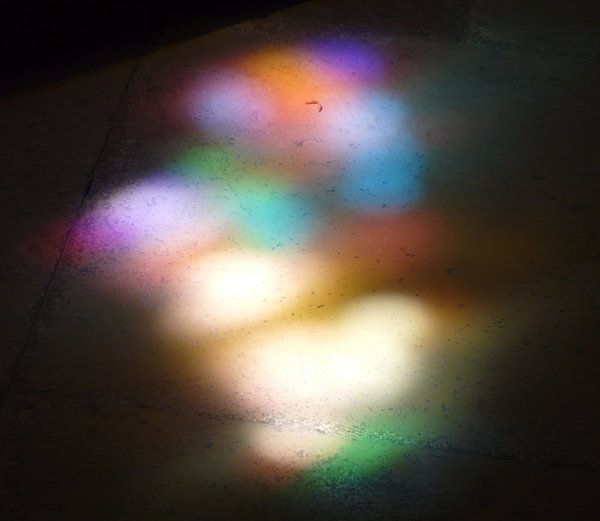
\includegraphics[height=4cm]{lichtspiel.jpg}
  \caption{标准的figure}
\end{figure}

\newtcolorbox[blend into=figures]{myfigure}[2][]{float=htb,capture=hbox,
  title={#2},every float=\centering,#1}

\begin{myfigure}{tcolorbox的figure}
  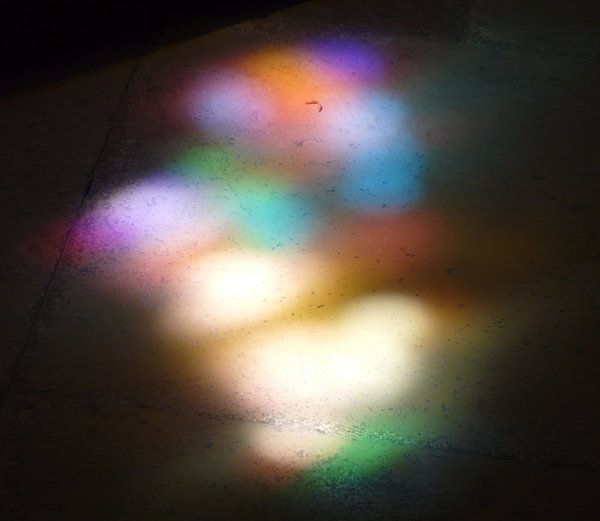
\includegraphics[height=4cm]{lichtspiel.jpg}
\end{myfigure}
\end{dispListing}
{\tcbusetemp}

% \clearpage
\begin{docTcbKey}[][doc new=2015-03-13]{blend before title}{=\meta{value}}{no default, initially \docValue{colon}}
\begin{stripedbox}
This option formats the title output of \refKeyLe{/tcb/new/blend into}.
Note that this is a common |tcolorbox| option which should be set
globally or in the normal option part of \refComLe{newtcolorbox}.
\tcblower
该选项用于格式化\refKeyLe{/tcb/new/blend into}的标题输出。%
注意,这是一个常见的 |tcolorbox| 选项,应该全局设置, 或在 \refComLe{newtcolorbox} 的普通选项部分。\end{stripedbox}

\begin{stripedbox}
Feasible values for \meta{value} are:
\tcblower
\meta{value}的可行值是:
\end{stripedbox}
\begin{itemize}
\item\docValue{colon}: 
\begin{stripedbox}
use name/number plus colon.
\tcblower
使用 |名字|/|编号| 加上 |冒号|
\end{stripedbox}

\item\docValue{dash}: 
\begin{stripedbox}
use name/number plus dash.
\tcblower
使用 |名字|/|编号| 加上 |破折号|
\end{stripedbox}

\item\docValue{colon hang}: 
\begin{stripedbox}
use name/number plus colon with hanging indent.
\tcblower
使用 |名字|/|编号| 加上 |冒号|,并悬挂式缩进。
\end{stripedbox}

\item\docValue{dash hang}: 
\begin{stripedbox}
use name/number plus dash with hanging indent.
\tcblower
使用 |名字|/|编号| 加上 |破折号|,并悬挂式缩进。
\end{stripedbox}
\end{itemize}

\begin{dispListing}
\newtcolorbox[blend into=figures]{myfigure}[2][]{float=htb,capture=hbox,
  blend before title=dash hang,title={#2},every float=\centering,#1}

\begin{myfigure}{一个标题相当长的tcolorbox图}
  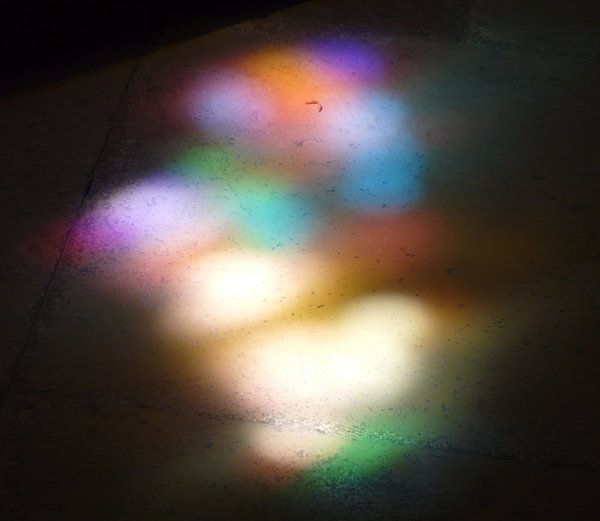
\includegraphics[height=5cm]{lichtspiel.jpg}
\end{myfigure}
\end{dispListing}
{\tcbusetemp}
\end{docTcbKey}

% \clearpage
\begin{docTcbKey}[][doc new=2015-03-13]{blend before title code}{=\meta{code}}{no default}
\begin{stripedbox}
This option formats the title output of \refKeyLe{/tcb/new/blend into}.
The \meta{code} takes one parameter, the name/number.
Use this, if \refKeyLe{/tcb/blend before title} is not flexible enough.
\tcblower
该选项格式化\refKeyLe{/tcb/new/blend into}的标题输出。%
\meta{code}接受一个参数,即 name/number。%
如果\refKeyLe{/tcb/blend before title}不够灵活,可以使用这个。
\end{stripedbox}

\begin{dispListing}
\newtcolorbox[blend into=figures]{myfigure}[2][]{float=htb,capture=hbox,
  blend before title code={\fbox{##1}\ },title={#2},every float=\centering,#1}

\begin{myfigure}{A tcolorbox figure}
  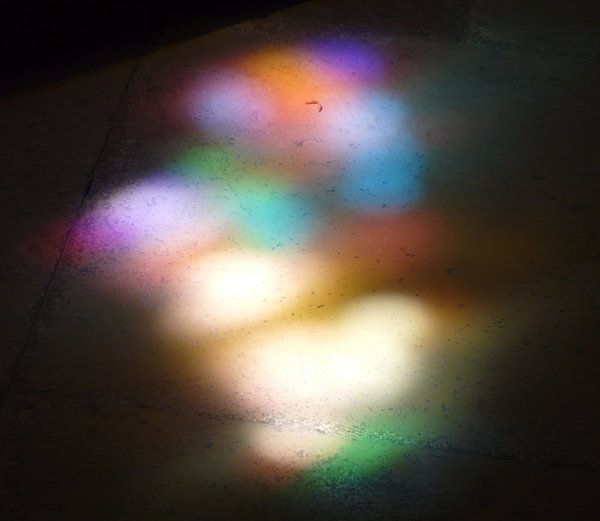
\includegraphics[height=6cm]{lichtspiel.jpg}
\end{myfigure}
\end{dispListing}
{\tcbusetemp}
\end{docTcbKey}

% \clearpage
% Lists of \texttt{tcolorbox}es
\subsection{\texttt{tcolorbox}盒子目录}\label{sec:listsof}
\begin{stripedbox}
For figures and tables, \LaTeX\ provides the |\listoffigures| and
|\listoftables| commands to create lists of these numbered entities.
Also, a |tcolorbox| can be part of such a kind of list.
\tcblower
对于图形和表格,\LaTeX\ 提供了 |\listfigures| 和 |\listoftables| 命令创建这些编号实体的列表。%
同样,|tcolorbox|可以是这种列表的一部分。
\end{stripedbox}

\begin{enumerate}
\item 
\begin{stripedbox}
Assign a list \meta{name} by the \emph{initialization} option
\refKeyLe{/tcb/new/list inside}.
\tcblower
通过\emph{初始化}选项\refKeyLe{/tcb/new/list inside}分配一个列表\meta{name}。
\end{stripedbox}

\item 
\begin{stripedbox}
Optionally, a new \meta{type} for list entries may be assigned
by the \emph{initialization} option \refKeyLe{/tcb/new/list type}.
\tcblower
可选地,通过\emph{初始化}选项\refKeyLe{/tcb/new/list type},%
可以为列表条目分配一个新的\meta{type}。
\end{stripedbox}

\item 
\begin{stripedbox}
List entries a generated automatically within each new |tcolorbox|
using the above initialization.
\tcblower
列出使用上述初始化在每个新|tcolorbox|中自动生成的条目。
\end{stripedbox}
    \begin{itemize}
    \item 
\begin{stripedbox}
If \refKeyLe{/tcb/list entry} is set, the entry is generated with it.
\tcblower
如果设置了\refKeyLe{/tcb/list entry},则生成该条目。
\end{stripedbox}
    
    \item 
\begin{stripedbox}
Otherwise, if \refKeyLe{/tcb/title} is set, the entry is generated with it.
\tcblower
否则,如果设置了\refKeyLe{/tcb/title},则生成该条目。
\end{stripedbox}
    
    \item 
\begin{stripedbox}
Otherwise, the entry is generated with the current number and the environment name.
\tcblower
否则,将使用当前编号和环境名称生成条目。
\end{stripedbox}
    
    \end{itemize}
\item 
\begin{stripedbox}
The generated list is displayed by \refComLe{tcblistof}.
\tcblower
生成的列表由\refComLe{tcblistof}显示。
\end{stripedbox}
\end{enumerate}

\begin{newTcbKey}{list inside}{=\meta{name}}{no default, initially unset}
\begin{stripedbox}
Assigns a list or contents file to the generated |tcolorbox|es.
Entries to this list are saved to a file which gets the \meta{name} as
file name extension. The list is referenced by this name in
\refComLe{tcblistof}.
For example:
\tcblower
为生成的 |tcolorbox| 盒子们分配一个列表或内容文件。%
此列表中的条目保存到一个文件中,该文件以\meta{name}作为文件扩展名。%
该列表由\refComLe{tcblistof}引用。%
例如:
\end{stripedbox}

\begin{dispListing}
list inside=exam
\end{dispListing}
\begin{stripedbox}
See Section \ref{listing:exercises} from page \pageref{listing:exercises}
for a complete example.
\tcblower
一个完整的例子参见 \pageref{listing:exercises} 页的 \ref{listing:exercises} 小节。
\end{stripedbox}
\end{newTcbKey}

\begin{newTcbKey}{list type}{=\meta{type}}{no default, initially |tcolorbox|}
\begin{stripedbox}
Optionally, some \meta{type} can be assigned to the list entries.
For a new \meta{type}, a macro |\l@|\meta{type} has to exist which controls
the format of the list entry. The default type is defined by
\tcblower
可选地,可以将列表条目设置为一些\meta{type}。%
对于一个新的\meta{type}, 存在宏命令 |\l@|\meta{type} 用于控制列表条目的格式。%
默认类型定义为:
\end{stripedbox}

\begin{dispListing}
\newcommand*\l@tcolorbox{\@dottedtocline{1}{1.5em}{2.3em}}
\end{dispListing}
\begin{stripedbox}
This is identical to the |\l@section| setting of \LaTeX. |\l@tcolorbox| can
be redefined or a new \meta{type} can be assigned.
\tcblower
这同 \LaTeX 的 |\l@section| 的定义是相同的。
|\l@tcolorbox| 可以重新定义或分配一个新的\meta{type}。
\end{stripedbox}
\end{newTcbKey}


% \clearpage
\begin{docCommand}[doc updated=2021-05-20]{tcblistof}{\oarg{macro}\marg{name}\oarg{short}\marg{title text}}
\begin{stripedbox}
Displays the generated list of |tcolorbox|es with the given \meta{name}.
The heading is generated by \meta{macro}\oarg{short}\marg{title text} where \texttt{\textbackslash section}
is the default setting for \meta{macro}.
Here, as usual, \meta{title text} is the title of the section or chapter
while \meta{short} is a shorter title for headings and table of contents.
\tcblower
用给定的\meta{name}显示生成的|tcolorbox|es列表。%
标题由\meta{macro}\oarg{short}\marg{title text}生成,其中\texttt{\textbackslash section} 是\meta{macro}的默认设置。%
这里,像往常一样,\meta{title text}是章或节的标题, \meta{short}是章或节的短标题.
\end{stripedbox}

\begin{itemize}
\item 
\begin{stripedbox}
If \meta{macro} ends with a |*|, \refComLe{tcblistof} mimics the behavior of
|\listoffigures| from the standard \LaTeX\ classes and adds the title
to the left and right mark for headings.
\tcblower
如果\meta{macro}以|*|结尾, \refComLe{tcblistof} 模拟标准 \LaTeX\ 的 |\listoffigures| 的行为,%
并将标题添加到页眉的左右标记。
\end{stripedbox}

\item 
\begin{stripedbox}
If \meta{macro} starts with |\chapter|, a possible two column document setting
is restored to one column (as standard \LaTeX\ classes do for |\listoffigures|).
\tcblower
如果\meta{macro}以|\chapter|开始, %
有一些的两列文档设置将恢复为一列 (像标准 \LaTeX\ 的 |\listoffigures| 做的那样).
\end{stripedbox}
\end{itemize}

\medskip
\begin{stripedbox}
To display the list inside a subsection, use for example:
\tcblower
要在subsection中显示列表,例如:
\end{stripedbox}
\begin{dispListing}
\tcblistof[\subsection]{exam}{List of Exercises}
\end{dispListing}
\begin{stripedbox}
The result of the example is found as Subsection \ref{listofexercises} on
page \pageref{listofexercises}.
\tcblower
示例结果可以参见在 \pageref{listofexercises} 页的 \ref{listofexercises} 小节。
\end{stripedbox}


\medskip
\begin{stripedbox}
To apply the list similar to |\listoffigures| for a report or book, use for example:
\tcblower
要将类似 |\listoffigures| 的列表应用于报告或书籍,请使用例如:
\end{stripedbox}
\begin{dispListing}
\tcblistof[\chapter*]{exam}{List of Exercises}
\end{dispListing}

\medskip
\begin{stripedbox}
To set a short title for headings with the default |\section| setting, use for example:
\tcblower
%todo 是页眉么?
使用默认|\section|设置,为页眉设置一个短标题,例如:
\end{stripedbox}
\begin{dispListing}
\tcblistof{exam}[List of Exercises]{Elaborate List of Fine Exercises
                                    for all Students of my Course}
\end{dispListing}

\medskip
\begin{marker}
\begin{stripedbox}
The core of the list is generated by |\@starttoc|\marg{name} which
can be wrapped into an own macro.
\tcblower
列表的核心是由|\@starttoc|\marg{name}生成的,%
可以包装到已有的宏。
\end{stripedbox}
\end{marker}
\end{docCommand}
%译 done 2023.1.23  5-initoptions
% \setcounter{section}{5}
% % !TeX root = tcolorbox.tex
% include file of tcolorbox.tex (manual of the LaTeX package tcolorbox)
% \clearpage
% Side by Side

\setcounter{section}{5}
\setcounter{subsection}{2}

\section{并排}\label{sec:sidebyside}%
\tcbset{external/prefix=external/sidebyside_}%

A \csh渐变盒子{side by side} box is a special \refEnvLe{tcolorbox} where
the upper and lower part of the box are set side by side.
All boxes of this kind are unbreakable.


一个\emph{并排}的盒子是一个特殊的\refEnvLe{tcolorbox},其中盒子的上部和下部并排设置。这种类型的所有盒子都是\csh渐变盒子[red]{不可分割的}。


\begin{marker}
% \begin{stripedbox}
Further side by side options for code examples are
% \tcblower

进一步的排版代码的 side by side 选项的例子有
% \end{stripedbox}

\refKeyLe{/tcb/listing side text},
\refKeyLe{/tcb/text side listing},
\refKeyLe{/tcb/listing outside text}, 和
\refKeyLe{/tcb/text outside listing}.
\end{marker}

% Basic Settings \hfill 
\subsection{基本设置}\label{subsec:sidebyside_basic}

% \begin{docTcbKey}{sidebyside}{=\colOpt{true\textbar false}}{默认值|true|,初始设置为|false|}
% \begin{docTcbKey}{sidebyside}{\colOpt{=true\textbar false}}{default |true|, initially |false|}
% \begin{stripedbox}
Normally, the upper part and the lower part of the box have their positions
as their names suggest. If |sidebyside| is set to |true|, the upper part
is drawn \emph{left-handed} and the lower part is drawn \emph{right-handed}.
Both parts are drawn together with the geometry settings of the upper part but the
space is divided horizontally according to the following options.
Colors, fonts, and box content additions are used individually.
The resulting box is unbreakable.

% Normally, the upper part and the lower part of the box have their positions as their names suggest. 
% 通常,盒子的upper部分和lower部分的位置,同它们的名字一致。%
% If |sidebyside| is set to |true|, the upper part
% is drawn \emph{left-handed} and the lower part is drawn \emph{right-handed}.
% 如果 |sidebyside| 设置为 true, 则upper部分会放置在左边,lower部分放置在右边。%

% Both parts are drawn together with the geometry settings of the upper part but the
% space is divided horizontally according to the following options.
% 两个部分都使用上部分的几何设置进行绘制,但空间按照以下选项水平分割。
% Colors, fonts, and box content additions are used individually.
% The resulting box is unbreakable.
% 颜色、字体和盒子内容的添加都是独立使用的。生成的盒子是\csh渐变盒子V[red]{不可分割}的。


通常,盒子的upper部分和lower部分的位置,同它们的名字一致。
如果 sidebyside 设置为 true, 则upper部分会放置在左边,lower部分放置在右边。
两个部分都使用上部分的几何设置进行绘制,但空间按照以下选项水平分割。颜色、字体和盒子内容的添加都是独立使用的。生成的盒子是\csh渐变盒子V[red]{不可分割}的。


\begin{dispExample}
\tcbset{colback=red!5!white%
,colframe=red!75!black%
,fonttitle=\bfseries}

\begin{tcolorbox}[title=我的标题,sidebyside]
这是 upper (\textit{左侧}) 部分。
\tcblower
这是 lower (\textit{右侧}) 部分。
\end{tcolorbox}
\end{dispExample}


%todo bicolor 是啥
\begin{dispExample}
% \usepackage{lipsum}
% \tcbuselibrary{skins}
\begin{tcolorbox}[bicolor% 表示创建一个双色盒子,即上下两部分的颜色可以不同。
,sidebyside%并排
,righthand width=3cm%指定右侧的宽度
,sharp corners,boxrule=.4pt,colback=green!5,colbacklower=green!50!black!50]
\lipsum[2]
\tcblower
\includegraphics[width=\linewidth]{goldshade}%
\end{tcolorbox}
\end{dispExample}
\end{docTcbKey}%
% % \clearpage
\begin{docTcbKey}[][doc updated=2015-02-06]{sidebyside align}{=\meta{alignment}}{no default, initially |center|}

Sets the vertical \meta{alignment} for the left-handed and right-handed part.%
Feasible values for \meta{alignment} are:

设置左侧和右侧的垂直 \meta{alignment} 方式。%
可选的 \meta{对齐} 值有:

\begin{tcolorbox}[title=\docValue{center},sidebyside,sidebyside align=center]
与 |minipage|环境的选项 |c| 相同。
\tcblower
identical to |minipage| option |c|.
\end{tcolorbox}
 
\begin{tcolorbox}[title=\docValue{top},sidebyside,sidebyside align=top]
与 |minipage| 选项 |t| 相同(根据基线对齐左侧和右侧的顶部行)。
\tcblower
identical to |minipage| option |t| (aligns the top lines of the left-handed and right-handed side according to their baselines).
\end{tcolorbox}

\begin{tcolorbox}[title=\docValue{bottom},sidebyside,sidebyside align=bottom]
与 |minipage| 选项 |b| 相同(根据基线对齐左侧和右侧的底部行)。
\tcblower
identical to |minipage| option |b| (aligns the bottom lines of the left-handed and right-handed side according to their baselines).
\end{tcolorbox}


\begin{tcolorbox}[title=\docValue{center seam},sidebyside,sidebyside align=center seam]
将左侧和右侧的中心对齐。
\tcblower
aligns the center of the left-handed and right-handed side.
\end{tcolorbox}

\begin{tcolorbox}[title=\docValue{top seam},sidebyside,sidebyside align=top seam]
将左侧和右侧的顶部接缝对齐。
\tcblower
aligns the very top seam of the left-handed and right-handed side.
\end{tcolorbox}


\begin{tcolorbox}[title=\docValue{bottom seam},sidebyside,sidebyside align=bottom seam]
将左侧和右侧的底部接缝对齐。
\tcblower
aligns the very bottom seam of the left-handed and right-handed side.
\end{tcolorbox}


% \begin{exdispExample}{sidebyside_align}
% \tcbset{colback=red!5!white,colframe=red!75!black,fonttitle=\bfseries,nobeforeafter,
%   left=2mm,right=2mm,sidebyside,sidebyside gap=6mm,width=(\linewidth-2mm)/3}

% \begin{tcolorbox}[adjusted title=center,sidebyside align=center]
% 这段文字太长了太长了太长了太长了,一行写不完。
% \tcblower
% 简短文字。
% \end{tcolorbox}\hfill
% \begin{tcolorbox}[adjusted title=top,sidebyside align=top]
% 这段文字太长了太长了太长了太长了,一行写不完。
% \tcblower
% 简短文字。
% \end{tcolorbox}\hfill
% \begin{tcolorbox}[adjusted title=bottom,sidebyside align=bottom]
% 这段文字太长了太长了太长了太长了,一行写不完。
% \tcblower
% 简短文字。
% \end{tcolorbox}
% \end{exdispExample}


% \begin{stripedbox}
\docValue{center}, \docValue{top}, and \docValue{bottom} are identical
to the known corresponding |minipage| options.
While this is the preferred approach for text content, the result for
boxed content like tables or images may not be as expected.
% \tcblower

\docValue{center}、\docValue{top}和\docValue{bottom}与 |minipage| 的选项相同。%
% 虽然这是文本内容的首选方法,%
% 对于盒子中是表格或图像等内容,结果可能与预期不同。
虽然这是文本内容的首选方法,但对于表格或图像等盒子内容的结果可能不如预期。
% \end{stripedbox}

% \begin{stripedbox}
For such content, one may use \docValue{center seam}, \docValue{top seam},
and \docValue{bottom seam}. For example, \docValue{top seam} aligns
the very top seam of the left-handed and right-handed side.
% \tcblower

% 对于这样的内容,可以使用\docValue{center seam}、\docValue{top seam}和\docValue{bottom seam},
% 例如,\docValue{top seam}对齐左和右边的最上面的缝。
% \end{stripedbox}

对于这样的内容,可以使用\docValue{center seam}、\docValue{top seam}和\docValue{bottom seam}。例如,\docValue{top seam}将左侧和右侧的顶部接缝对齐。


\begin{dispExample}
\tcbset{colback=red!5!white,colframe=red!75!black,fonttitle=\bfseries,
  size=small,righthand width=4cm,sidebyside,sidebyside gap=6mm,lower separated=false}

\begin{tcolorbox}[adjusted title=center seam,sidebyside align=center seam]
This is my description text for the pictures displayed on the right-handed side.
\tcblower
\includegraphics[width=\linewidth/2]{goldshade}%
\includegraphics[width=\linewidth/2]{blueshade}
\end{tcolorbox}

\begin{tcolorbox}[adjusted title=top seam,sidebyside align=top seam]
  This is my description text for the pictures displayed on the right-handed side.
  \tcblower
  \includegraphics[width=\linewidth/2]{goldshade}%
  \includegraphics[width=\linewidth/2]{blueshade}
\end{tcolorbox}

\begin{tcolorbox}[adjusted title=bottom seam,sidebyside align=bottom seam]
  This is my description text for the pictures displayed on the right-handed side.
  \tcblower
  \includegraphics[width=\linewidth/2]{goldshade}%
  \includegraphics[width=\linewidth/2]{blueshade}
\end{tcolorbox}
\end{dispExample}
\end{docTcbKey}%
% % \clearpage
\begin{docTcbKey}{sidebyside gap}{=\meta{length}}{no default, initially |10mm|}
% \begin{stripedbox}
Sets the horizontal distance between the left-handed and right-handed part to \meta{length}.
% \tcblower

将左和右部分之间的水平距离设置为\meta{length}。
% \end{stripedbox}

\begin{dispExample}
\tcbset{colback=red!5!white,colframe=red!75!black,fonttitle=\bfseries,nobeforeafter,
  sidebyside,width=(\linewidth-2mm)/2}

\begin{tcolorbox}[adjusted title=宽gap,sidebyside gap=30mm]
这段文字太长了太长了太长了太长了,一行写不完。
\tcblower
简短文字。
\end{tcolorbox}\hfill
\begin{tcolorbox}[adjusted title=窄gap,sidebyside gap=1mm]
这段文字太长了太长了太长了太长了,一行写不完。
\tcblower
简短文字
\end{tcolorbox}
\end{dispExample}
\end{docTcbKey}%
% \begin{docTcbKey}{lefthand width}{=\meta{length}}{no default, initially unset}

Sets the width of the left-handed part to the given \meta{length}.

将左部的宽度设置为给定的\meta{length}。


\begin{dispExample}
\tcbset{colback=red!5!white,colframe=red!75!black,fonttitle=\bfseries}

\begin{tcolorbox}[title=My title,sidebyside,lefthand width=3cm]
这是 upper (\textit{左}) 部分.
\tcblower
这是 lower (\textit{右}) 部分.
\end{tcolorbox}
\end{dispExample}
\end{docTcbKey}

\enlargethispage*{1cm}
\begin{docTcbKey}{righthand width}{=\meta{length}}{no default, initially unset}

Sets the width of the right-handed part to the given \meta{length}.

将右部的宽度设置为给定的\meta{length}。


\begin{dispExample}
\tcbset{colback=red!5!white,colframe=red!75!black,fonttitle=\bfseries}

\begin{tcolorbox}[title=My title,sidebyside,righthand width=3cm]
这是 upper (\textit{左}) 部分.
\tcblower
这是 lower (\textit{右}) 部分.
\end{tcolorbox}
\end{dispExample}
\end{docTcbKey}

% \clearpage
\begin{docTcbKey}{lefthand ratio}{=\meta{fraction}}{no default, initially |0.5|}

Sets the width of the left-handed part to the given \meta{fraction} of
the available space. \meta{fraction} is a value between |0| and |1|.

设置左侧的宽度为所有可用宽度的比例 \meta{fraction}。
\meta{fraction} 取值在 |0| 到 |1|。


\begin{dispExample}
\tcbset{colback=red!5!white,colframe=red!75!black,fonttitle=\bfseries}

\begin{tcolorbox}[title=My title,sidebyside,lefthand ratio=0.25]
这是 upper (\textit{左}) 部分.
\tcblower
这是 lower (\textit{右}) 部分.
\end{tcolorbox}
\end{dispExample}
\end{docTcbKey}


\begin{docTcbKey}{righthand ratio}{=\meta{fraction}}{no default, initially |0.5|}

Sets the width of the right-handed part to the given \meta{fraction} of
the available space. \meta{fraction} is a value between |0| and |1|.

设置右侧的宽度为所有可用宽度的比例 \meta{fraction}。
\meta{fraction} 取值在 |0| 到 |1|。


\begin{dispExample}
\tcbset{colback=red!5!white,colframe=red!75!black,fonttitle=\bfseries}
\begin{tcolorbox}[title=My title,sidebyside,righthand ratio=0.25]
这是 upper (\textit{左}) 部分.
\tcblower
这是 lower (\textit{右}) 部分.
\end{tcolorbox}
\end{dispExample}
\end{docTcbKey}


% \clearpage

If one side of a side-by-side box should be adapted to the width of its content, 
this width has to be computed beforehand.
The following example uses a savebox |\mysavebox| to store the picture to determine its width. 
A more convenient way to handle this task is to use the methods from \Fullref{subsec:sidebyside_xparse}.

如果一个并排的盒子的一边要适应其内容的宽度, %
这个宽度必须事先计算。%
下面的例子使用一个存储盒子 |\mysavebox| 来存储图片以确定其宽度。%
处理这个任务更方便的方法是使用来自 \Fullref{subsec:sidebyside_xparse} 的方法。

\begin{引述之言}{virhuiai}
可以在code中处理,见下面的例子。
\end{引述之言}
% code={\sbox{\mysavebox}{#2}},
% lefthand width=\wd\mysavebox,

\begin{dispExample}
% \tcbuselibrary{skins,xparse}
% \usepackage{lipsum}
% \newsavebox\mysavebox  % preamble
\DeclareTotalTColorBox{\mysidebox}{ O{} +m +m }{
  bicolor,colback=white,colbacklower=yellow!10,
  fonttitle=\bfseries,center title,
  sidebyside,
  code={\sbox{\mysavebox}{#2}},
  lefthand width=\wd\mysavebox,
  drop lifted shadow,
  #1
}
{\usebox{\mysavebox}\tcblower#3}

\mysidebox[title=The Triangle]{%
  \begin{tikzpicture}
    \path[fill=red!20,draw=red!50!black]
      (0,0) node[below]{A} -- (3,1) node[right]{B}
      -- (1,4) node[above]{C} -- cycle;
  \end{tikzpicture}%
}{%
  \lipsum[1]
} 
\end{dispExample}% % code={\sbox{\mysavebox}{#2}}, % lefthand width=\wd\mysavebox, 学习了

% % \clearpage
% Advanced Settings from the \mylib{xparse} Library
\subsection{来自\mylib{xparse}库的高级设置}\label{subsec:sidebyside_xparse}

\begin{marker}

All following macros and options need the \mylib{xparse} library to be
loaded, see \Fullref{sec:xparse}.

所有下面的宏和选项都需要加载 \mylib{xparse}库,见\Fullref{sec:xparse}。

\end{marker}


\begin{docCommand}[doc new=2015-11-20]{tcbsidebyside}{\oarg{options}\marg{left-handed content}\marg{right-handed content}}

Creates a colored box using more or less arbitrary \meta{options} for a \refEnvLe{tcolorbox}.
The \refKeyLe{/tcb/sidebyside} option is set to |true| and the \meta{left-handed content} and \meta{right-handed content} is filled into the box appropriately.
The resulting box is unbreakable.

% 为\refEnvLe{tcolorbox}指定任意的选项\meta{options}创建一个 |tcolorbox| 盒子。%
% \refKeyLe{/tcb/sidebyside}选项被设置为|true|, \meta{left-handed content}和\meta{right-handed content}被适当地填充到盒子中。%
% 这样的盒子是不可分页的。

使用更多或更少任意的\meta{选项}创建一个带有\refEnvLe{tcolorbox}的盒子。
\refKey{/tcb/sidebyside}选项设置为|true|,\meta{左侧内容}和\meta{右侧内容}被适当地填充到盒子中。
生成的盒子不可分割。



\refComLe{tcbsidebyside} is not only a shortcut for using a normal \refEnvLe{tcolorbox} with \refKeyLe{/tcb/sidebyside}, 
but allows setting further options like \refKeyLe{/tcb/sidebyside adapt} and \refKeyLe{/tcb/sidebyside switch}.

% \refComLe{tcbsidebyside}不只是使用普通的\refEnvLe{tcolorbox}指定\refKeyLe{/tcb/sidebyside}的快捷方式, 
% 还允许设置更多的选项,如\refKeyLe{/tcb/sidebyside adapt}和\refKeyLe{/tcb/sidebyside switch}。
\refComLe{tcbsidebyside}不仅是使用普通\refEnvLe{tcolorbox}与\refKeyLe{/tcb/sidebyside}的快捷方式,还允许设置其他选项,如\refKeyLe{/tcb/sidebyside adapt}和\refKeyLe{/tcb/sidebyside switch}。

\begin{dispExample}
% \tcbuselibrary{skins,xparse}
% \usepackage{lipsum}
\tcbsidebyside[title=The Triangle,
  sidebyside adapt=left,
  bicolor,colback=white,colbacklower=yellow!10,
  fonttitle=\bfseries,center title,drop lifted shadow,
]{%
  \begin{tikzpicture}
    \path[fill=red!20,draw=red!50!black]
      (0,0) node[below]{A} -- (3,1) node[right]{B}
      -- (1,4) node[above]{C} -- cycle;
  \end{tikzpicture}%
}{%
  \lipsum[1]
}
\end{dispExample}

\begin{dispExample*}{}
\tcbsidebyside[title={sidebyside adapt=left \hfill 左侧变成能不换行的了---virhuiai},
sidebyside adapt=left,
bicolor,colback=white,colbacklower=yellow!10,
fonttitle=\bfseries,center title,drop lifted shadow,
]{农夫倦步长道回家,

仅余我与暮色平分此世界。}{The ploughman

homeward plods his weary way,

And leaves the world

to darkness and to me.
}
\end{dispExample*}
\end{docCommand}%\subsection{来自\mylib{xparse}库的高级设置}



key_sidebyside_adapt



 
\end{document}

 


% \clearpage
\begin{docTcbKey}[][doc new=2015-11-20]{sidebyside adapt}{=\meta{side(s)}}{no default, initially |none|}
\begin{stripedbox}
The option allows the left-handed and/or right-handed side to determine the dimensions of the box. 
This option is only valid inside \refComLe{tcbsidebyside}.
\tcblower
该选项允许根据左边和/右边内容确定盒子的尺寸。
此选项仅在\refComLe{tcbsidebyside}内有效。
\end{stripedbox}

Feasible values for \meta{side(s)} are:
\begin{itemize}
    \item\docValue{none}: 
\begin{stripedbox}
no measurement of left-handed and right-handed side.
\tcblower
不测量左边和右边。
\end{stripedbox}
    \item\docValue{left}:
\begin{stripedbox}
the actual width of the left-handed content is used to set \refKeyLe{/tcb/lefthand width}.
\tcblower
左侧内容的实际宽度用于设置 \refKeyLe{/tcb/lefthand width}。
\end{stripedbox}
    \item\docValue{right}:
\begin{stripedbox}
the actual width of the right-handed content is used to set \refKeyLe{/tcb/righthand width}.
\tcblower
右侧内容的实际宽度用于设置\refKeyLe{/tcb/右手宽度}。
\end{stripedbox}

    \item\docValue{both}:
\begin{stripedbox}
the actual width of the left-handed and right-handed content is used to set \refKeyLe{/tcb/lefthand width},  \refKeyLe{/tcb/righthand width}, and the overall \refKeyLe{/tcb/width}.
\tcblower
左手和右手内容的实际宽度用于设置 \refKeyLe{/tcb/lefthand width} 和 \refKeyLe{/tcb/righthand width},%
和整个\refKeyLe{/tcb/width}。
\end{stripedbox}

\end{itemize}

\begin{dispExample}
% \tcbuselibrary{skins,xparse}
\tcbsidebyside[sidebyside adapt=left,
  title=非常重要的表格,
  beamer,colframe=blue!50!black,colback=blue!10
  ,lower separated=false%无分隔线了
  ,sidebyside gap=5mm
]{%
  \begin{tabular}{|l|c|r|}\hline
    left & center & right\\\hline
    A & B & C\\\hline
    D & E & F\\\hline
  \end{tabular}
}{%
此表包含所有未来操作的最重要数据。
你可能注意到B跟在A后面,C跟在B后面,以此类推。
}
\end{dispExample}



\begin{dispExample}
% \tcbuselibrary{skins,xparse}
\tcbsidebyside[sidebyside adapt=right,
  blanker,sidebyside gap=5mm
]{%
  \lipsum[2]
}{%
\begin{tikzpicture}
  \path[fill=yellow,draw=yellow!75!red] (0,0) circle (1cm);
  \fill[red] (45:5mm) circle (1mm);
  \fill[red] (135:5mm) circle (1mm);
  \draw[line width=1mm,red] (215:5mm) arc (215:325:5mm);
\end{tikzpicture}
}
\end{dispExample}


\begin{dispExample}
% \tcbuselibrary{skins,xparse}
\tcbsidebyside[sidebyside adapt=both,
  enhanced,center,
  title=Both sides adapted,
  attach boxed title to top center={yshift=-2mm},
  coltitle=black,boxed title style={colback=red!25},
  segmentation style=solid,colback=red!5,colframe=red!50
]{%
  \begin{tabular}{|l|c|r|}\hline
    left & center & right\\\hline
    A & B & C\\\hline
    D & E & F\\\hline
  \end{tabular}
}{%
\begin{tikzpicture}
  \path[fill=yellow,draw=yellow!75!red] (0,0) circle (1cm);
  \fill[red] (45:5mm) circle (1mm);
  \fill[red] (135:5mm) circle (1mm);
  \draw[line width=1mm,red] (215:5mm) arc (215:325:5mm);
\end{tikzpicture}
}
\end{dispExample}
\end{docTcbKey}

% \clearpage
\begin{docTcbKey}[][doc new=2015-11-20]{sidebyside switch}{\colOpt{=true\textbar false}}{default |true|, initially |false|}
\begin{stripedbox}
If set to |true|, the
\meta{left-handed content} and \meta{right-handed content}
of \refComLe{tcbsidebyside} are switched.
Obviously, this option is only valid inside \refComLe{tcbsidebyside}.
\tcblower
如果设置为|true|,%
\refComLe{tcbsidebyside}的 \meta{left-handed content} 和 \meta{right-handed content} 会被切换。%
显然,这个选项只在\refComLe{tcbsidebyside}内有效。
\end{stripedbox}

\begin{stripedbox}
The side switching can be made even/odd page sensitive, 
if used inside \refKeyLe{/tcb/if odd page}.
\tcblower
如果指定了了 \refKeyLe{/tcb/if odd page},两侧切换对奇/偶页敏感。
\end{stripedbox}


\begin{dispExample}
% \tcbuselibrary{skins,xparse}
\tcbsidebyside{Left}{Right}

\tcbsidebyside[sidebyside switch]{Left}{Right}

\tcbsidebyside[title=Very important table,
  if odd page={sidebyside switch,sidebyside adapt=right,flushright title}%
              {sidebyside adapt=left},
  beamer,colframe=blue!50!black,colback=blue!10,
  lower separated=false,sidebyside gap=5mm
]{%
  \begin{tabular}{|l|c|r|}\hline
    left & center & right\\\hline
    A & B & C\\\hline
    D & E & F\\\hline
  \end{tabular}
}{%
  This table contains the most important figures for
  all future actions. You may notice that B follows A,
  C follows B, and so on.
}
\end{dispExample}


\end{docTcbKey}

%译 done 2023.1.23
% \setcounter{section}{6}
% \include*{tcolorbox.doc.verbatim}%译 done 2023.1.23|v2 20230325
% \include*{tcolorbox.doc.recording}%%译 done 2023.1.24|v2 20230325

% \setcounter{section}{8}
% \include*{tcolorbox.doc.technical}%todo 不必要,如何只是使用


% \include*{tcolorbox.doc.skins}%todo 翻译了一些 TODo

% \setcounter{section}{10}
% % !TeX root = tcolorbox.tex
% include file of tcolorbox.tex (manual of the LaTeX package tcolorbox)
\clearpage
\section{Library \mylib{skins} - Catalog of Skins}\label{sec:skincatalog}%
\tcbset{external/prefix=external/skincatalog_}%
The \mylib{skins} library provides a catalog of skins to choose from which
is documented in the following. The \mylib{skins} library has to be loaded
by a package option or inside the preamble by:
\begin{dispListing}
\tcbuselibrary{skins}
\end{dispListing}

See \Vref{sec:skins} for the documentation of all other options of the \mylib{skins} library.

\begin{itemize}
\item In principle, a skin is applied by choosing a value for
  \refKeyLe{/tcb/skin}, e.g. \docValue*{enhanced}.
  Since the parts of a breakable box should look different,
  there are individual skins for breakable boxes, also see \Vref{subsec:breaksequence}.
  Skins for breakable boxes derived from a base skin are called a skin family
  in the following.
\item Instead of setting values for \refKeyLe{/tcb/skin}, equally named options
  can be used which are shortcuts and which sometimes also change some
  geometry or style settings. These are the intended options for normal users.
  Typically, one of the following options is sufficient to select a skin:
  \begin{itemize}
  \item \refKeyLe{/tcb/standard}
  \item \refKeyLe{/tcb/standard jigsaw}
  \item \refKeyLe{/tcb/enhanced}
  \item \refKeyLe{/tcb/enhanced jigsaw}
  \item \refKeyLe{/tcb/enhanced standard}
  \item \refKeyLe{/tcb/enhanced standard jigsaw}
  \item \refKeyLe{/tcb/bicolor}
  \item \refKeyLe{/tcb/tile}
  \item \refKeyLe{/tcb/beamer}
  \item \refKeyLe{/tcb/widget}
  \item \refKeyLe{/tcb/empty}
  \item \refKeyLe{/tcb/spartan}
  \item \refKeyLe{/tcb/draft}
  \end{itemize}
  Additionally, there are some special applications:
  \begin{itemize}
  \item \refKeyLe{/tcb/marker}
  \item \refKeyLe{/tcb/blank}
  \item \refKeyLe{/tcb/blanker}
  \item \refKeyLe{/tcb/blankest}
  \end{itemize}
\end{itemize}



\clearpage

The auxiliary macro \docAuxCommand{skinExampleSet} is used for the
following examples to display skin applications. Note that
\docAuxCommand{skinExampleSet} is not part of the package, but is
defined just for this documentation.

\begin{dispListing}
\NewDocumentCommand{\skinExampleSet}{m}{%
  \begin{tcbraster}[raster equal height,raster columns=3,
      colback=LightGreen,colframe=DarkGreen,colbacktitle=LimeGreen!75!DarkGreen,
      #1,
      left=1mm,right=1mm,top=1mm,bottom=1mm,middle=1mm,
      sidebyside gap=4mm]
    \begin{tcolorbox}
      This is my content.
    \end{tcolorbox}
    \begin{tcolorbox}
      This is my content.
      \tcblower
      More content.
    \end{tcolorbox}
    \begin{tcolorbox}[sidebyside]
      My content.
      \tcblower
      More content.
    \end{tcolorbox}
    \begin{tcolorbox}[adjusted title=My title]
      This is my content.
    \end{tcolorbox}
    \begin{tcolorbox}[adjusted title=My title]
      This is my content.
      \tcblower
      More content.
    \end{tcolorbox}
    \begin{tcolorbox}[adjusted title=My title,sidebyside]
      My content.
      \tcblower
      More content.
    \end{tcolorbox}
  \end{tcbraster}
}
\end{dispListing}
\tcbusetemp


\clearpage
\tcbset{skintable/.style={colframe=red!50!yellow!50!black,
  colback=red!50!yellow!5!white,coltitle=red!50!yellow!3!white,
  fonttitle=\bfseries,before=\par\smallskip,
  title=Environment and engines for the skin \enquote{\texttt{#1}}}}

\subsection{Skin Family \enquote{standard}}\label{subsec:skinstandard}
\begin{marker}Note that the option keys \refKeyLe{/tcb/frame style},
  \refKeyLe{/tcb/interior style},
  \refKeyLe{/tcb/segmentation style}, and
  \refKeyLe{/tcb/title style} are not be applicable to the standard skin.
  Also, watermarks (see Subsection \ref{subsec:watermarks})
  are not usable with the standard skin.
\end{marker}

\begin{docSkin}{standard}
  This is the standard skin from the core package. All drawing engines
  are set to type |standard|. The drawing is based on |pgf| commands and
  does not need the |tikz| package.
\begin{tcolorbox}[skintable=standard]
  \begin{tabbing}
    \refKeyLe{/tcb/interior titled engine}: \=\kill
    \refKeyLe{/tcb/graphical environment}:  \> |pgfpicture|\\ 
    \refKeyLe{/tcb/frame engine}:           \> |standard|\\
    \refKeyLe{/tcb/interior titled engine}: \> |standard|\\ 
    \refKeyLe{/tcb/interior engine}:        \> |standard|\\
    \refKeyLe{/tcb/segmentation engine}:    \> |standard|\\
    \refKeyLe{/tcb/title engine}:           \> |standard|
  \end{tabbing}
\end{tcolorbox}
\end{docSkin}

\begin{docTcbKey}{standard}{}{style, no value}
  This is an abbreviation for setting |skin=standard|.
\end{docTcbKey}

\begin{dispExample}
\skinExampleSet{standard}
\end{dispExample}

\clearpage

\begin{docSkin}{standard jigsaw}
  This is the standard jigsaw skin from the core package. It differs from
  the skin \refSkin{standard} by its frame engine, see \Vref{subsec:skinjigsaw}.
\begin{tcolorbox}[skintable=standard jigsaw]
  \begin{tabbing}
    \refKeyLe{/tcb/interior titled engine}: \=\kill
    \refKeyLe{/tcb/graphical environment}:  \> |pgfpicture|\\ 
    \refKeyLe{/tcb/frame engine}:           \> |standardjigsaw|\\
    \refKeyLe{/tcb/interior titled engine}: \> |standard|\\ 
    \refKeyLe{/tcb/interior engine}:        \> |standard|\\
    \refKeyLe{/tcb/segmentation engine}:    \> |standard|\\
    \refKeyLe{/tcb/title engine}:           \> |standard|
  \end{tabbing}
\end{tcolorbox}
\end{docSkin}

\begin{docTcbKey}{standard jigsaw}{}{style, no value}
  This is an abbreviation for setting |skin=standard jigsaw|.
\end{docTcbKey}

\begin{dispExample*}{segmentation style={preaction={fill=white},pattern=checkerboard,pattern color=gray!40}}
\skinExampleSet{standard jigsaw,
  opacityframe=0.5,opacityback=0.5,opacitybacktitle=0.5,
}
\end{dispExample*}


\clearpage
\subsection{Skin Family \enquote{enhanced}}
\begin{marker}
If you like the standard appearance of a |tcolorbox| but you want to
have some \enquote{enhanced} features, the |enhanced| skin is what you are looking for.
\end{marker}

\begin{docSkin}{enhanced}
  This skin translates the drawing commands of the core package into |tikz|
  path commands. Therefore, it allows all |tikz| high level options for
  these paths and has more flexibility compared to the \refSkin{standard} skin.
  You pay for this with some prolonged compilation time.
  The |tikz| path options can
  be given with the option keys
  \refKeyLe{/tcb/frame style},
  \refKeyLe{/tcb/interior style},
  \refKeyLe{/tcb/segmentation style}, and
  \refKeyLe{/tcb/title style}.
\begin{tcolorbox}[skintable=enhanced]
  \begin{tabbing}
    \refKeyLe{/tcb/interior titled engine}: \=\kill
    \refKeyLe{/tcb/graphical environment}:  \> |tikzpicture|\\ 
    \refKeyLe{/tcb/frame engine}:           \> |path|\\
    \refKeyLe{/tcb/interior titled engine}: \> |path|\\ 
    \refKeyLe{/tcb/interior engine}:        \> |path|\\
    \refKeyLe{/tcb/segmentation engine}:    \> |path|\\
    \refKeyLe{/tcb/title engine}:           \> |path|
  \end{tabbing}
\end{tcolorbox}
\end{docSkin}


\begin{docTcbKey}{enhanced}{}{style, no value}
  This is an abbreviation for setting |skin=enhanced|.
\end{docTcbKey}

\begin{dispExample}
\skinExampleSet{enhanced}
\end{dispExample}

\clearpage

\begin{dispExample}
% \usetikzlibrary{shadings}         % preamble
\tcbset{skin=enhanced,fonttitle=\bfseries,
  frame style={upper left=blue,upper right=red,lower left=yellow,lower right=green},
  interior style={white,opacity=0.5},
  segmentation style={black,solid,opacity=0.2,line width=1pt}}

\begin{tcolorbox}[title=Nice box in rainbow colors]
  With the \enquote{enhanced} skin, it is quite easy to produce fancy looking effects.
  \tcblower
  Note that this is still a \texttt{tcolorbox}.
\end{tcolorbox}
\end{dispExample}


\begin{dispExample}
% \usetikzlibrary{decorations.pathmorphing} % preamble
\tcbset{skin=enhanced,fonttitle=\bfseries,boxrule=1mm,
  frame style={draw=FireBrick,fill=Salmon},drop fuzzy shadow,
  interior style={draw=FireBrick,top color=Salmon!10,bottom color=Salmon!20},
  segmentation style={draw=FireBrick,solid,decorate,
        decoration={coil,aspect=0,segment length=10.1mm}}}

\begin{tcblisting}{title=A listing box with shadow and some specials}
Of course, skins can be used for listings also.
\begin{equation}
  \int\limits_1^2 \frac{1}{x}~dx = \ln(2).
\end{equation}
\end{tcblisting}
\end{dispExample}


\clearpage


\begin{docTcbKey}{enhanced standard}{}{style, no value}
  For unbreakable boxes, this is identical to using \refKeyLe{/tcb/enhanced}.
  But, for breakable boxes, the \emph{break sequence} is identical to the \refSkin{standard} skin,
  see Section \ref{subsec:breaksequence} from page \pageref{subsec:breaksequence}.
\end{docTcbKey}


\begin{docTcbKey}{blank}{}{style, initially unset}
  This style relies on the skin \refSkin{enhanced}. All drawing operations
  are hidden and all margins are set to |0pt|. See \refKeyLe{/tcb/blanker}
  for switching off the drawing engines.
\begin{dispExample}
\begin{tcolorbox}[blank,watermark text=A blank box]
\lipsum[1]
\end{tcolorbox}
\end{dispExample}
\end{docTcbKey}

\clearpage
\begin{docCommand}{tcbline}{}
  Sometimes, a line is only a line. With \refComLe{tcblower} you separate
  the box content into two functional units. |\tcbline| draws only a line
  which looks like the segmentation line between upper and lower part.
  Furthermore, you can use |\tcbline| more than just once.
  |\tcbline| always uses the |path| drawing engine. Therefore,
  the \refKeyLe{/tcb/segmentation style} can be applied.

\begin{dispExample}
\tcbset{enhanced,colframe=blue!50!black,colback=white}

\begin{tcolorbox}[colupper=red!50!black,collower=green!50!black]
\lipsum[1]
\tcbline
\lipsum[2]
\tcblower
\lipsum[3]
\tcbline
\lipsum[4]
\end{tcolorbox}
\end{dispExample}
\end{docCommand}

\begin{docCommand}{tcbline*}{}
  Equivalent to \refComLe{tcbline}, but in a breakable box, \refComLe{tcbline*}
  is removed if at a page/box break. Also, it is removed at the end
  of a box.
\end{docCommand}

\clearpage
\begin{docSkin}{enhancedfirst}
This is a flavor of \refSkin{enhanced} which is used as a \emph{first} part
in a break sequence for \refSkin{enhanced}.
Nevertheless, this skin can be applied independently.
\begin{tcolorbox}[skintable=enhancedfirst]
  \begin{tabbing}
    \refKeyLe{/tcb/interior titled engine}: \=\kill
    \refKeyLe{/tcb/graphical environment}:  \> |tikzpicture|\\ 
    \refKeyLe{/tcb/frame engine}:           \> |pathfirst|\\
    \refKeyLe{/tcb/interior titled engine}: \> |pathfirst|\\ 
    \refKeyLe{/tcb/interior engine}:        \> |pathfirst|\\
    \refKeyLe{/tcb/segmentation engine}:    \> |path|\\
    \refKeyLe{/tcb/title engine}:           \> |pathfirst|
  \end{tabbing}
\end{tcolorbox}
\end{docSkin}


\begin{dispExample}
\skinExampleSet{skin=enhancedfirst}
\end{dispExample}

\medskip

%\clearpage
\begin{docSkin}{enhancedmiddle}
This is a flavor of \refSkin{enhanced} which is used as a \emph{middle} part
in a break sequence for \refSkin{enhanced}.
Nevertheless, this skin can be applied independently.
\begin{tcolorbox}[skintable=enhancedmiddle]
  \begin{tabbing}
    \refKeyLe{/tcb/interior titled engine}: \=\kill
    \refKeyLe{/tcb/graphical environment}:  \> |tikzpicture|\\ 
    \refKeyLe{/tcb/frame engine}:           \> |pathmiddle|\\
    \refKeyLe{/tcb/interior titled engine}: \> |pathmiddle|\\ 
    \refKeyLe{/tcb/interior engine}:        \> |pathmiddle|\\
    \refKeyLe{/tcb/segmentation engine}:    \> |path|\\
    \refKeyLe{/tcb/title engine}:           \> |pathmiddle|
  \end{tabbing}
\end{tcolorbox}
\end{docSkin}


\begin{dispExample}
\skinExampleSet{skin=enhancedmiddle}
\end{dispExample}


\clearpage
\begin{docSkin}{enhancedlast}
This is a flavor of \refSkin{enhanced} which is used as a \emph{last} part
in a break sequence for \refSkin{enhanced}.
Nevertheless, this skin can be applied independently.
\begin{tcolorbox}[skintable=enhancedlast]
  \begin{tabbing}
    \refKeyLe{/tcb/interior titled engine}: \=\kill
    \refKeyLe{/tcb/graphical environment}:  \> |tikzpicture|\\ 
    \refKeyLe{/tcb/frame engine}:           \> |pathlast|\\
    \refKeyLe{/tcb/interior titled engine}: \> |pathlast|\\ 
    \refKeyLe{/tcb/interior engine}:        \> |pathlast|\\
    \refKeyLe{/tcb/segmentation engine}:    \> |path|\\
    \refKeyLe{/tcb/title engine}:           \> |pathlast|
  \end{tabbing}
\end{tcolorbox}
\end{docSkin}

\begin{dispExample}
\skinExampleSet{skin=enhancedlast}
\end{dispExample}

\clearpage

\begin{docSkin}{enhanced jigsaw}
  This is the jigsaw variant of skin \refSkin{enhanced}.
  It differs by its frame engine, see \Vref{subsec:skinjigsaw}.
\begin{tcolorbox}[skintable=enhanced jigsaw]
  \begin{tabbing}
    \refKeyLe{/tcb/interior titled engine}: \=\kill
    \refKeyLe{/tcb/graphical environment}:  \> |tikzpicture|\\ 
    \refKeyLe{/tcb/frame engine}:           \> |pathjigsaw|\\
    \refKeyLe{/tcb/interior titled engine}: \> |path|\\ 
    \refKeyLe{/tcb/interior engine}:        \> |path|\\
    \refKeyLe{/tcb/segmentation engine}:    \> |path|\\
    \refKeyLe{/tcb/title engine}:           \> |path|
  \end{tabbing}
\end{tcolorbox}
\end{docSkin}

\begin{docTcbKey}{enhanced jigsaw}{}{style, no value}
  This is an abbreviation for setting |skin=enhanced jigsaw|.
\end{docTcbKey}


\begin{dispExample*}{segmentation style={preaction={fill=white},pattern=checkerboard,pattern color=gray!40}}
\skinExampleSet{enhanced jigsaw,
  opacityframe=0.5,opacityback=0.5,opacitybacktitle=0.5,
}
\end{dispExample*}


\begin{docTcbKey}[][doc new=2017-07-01]{enhanced standard jigsaw}{}{style, no value}
  For unbreakable boxes, this is identical to using \refKeyLe{/tcb/enhanced jigsaw}.
  But, for breakable boxes, the \emph{break sequence} is identical to the \refSkin{standard jigsaw} skin,
  see Section \ref{subsec:breaksequence} from page \pageref{subsec:breaksequence}.
\end{docTcbKey}


\clearpage
\begin{docSkin}{enhancedfirst jigsaw}
  This is the jigsaw variant of skin \refSkin{enhancedfirst}.
  It differs by its frame engine, see \Vref{subsec:skinjigsaw}.
\begin{tcolorbox}[skintable=enhancedfirst jigsaw]
  \begin{tabbing}
    \refKeyLe{/tcb/interior titled engine}: \=\kill
    \refKeyLe{/tcb/graphical environment}:  \> |tikzpicture|\\ 
    \refKeyLe{/tcb/frame engine}:           \> |pathfirstjigsaw|\\
    \refKeyLe{/tcb/interior titled engine}: \> |pathfirst|\\ 
    \refKeyLe{/tcb/interior engine}:        \> |pathfirst|\\
    \refKeyLe{/tcb/segmentation engine}:    \> |path|\\
    \refKeyLe{/tcb/title engine}:           \> |pathfirst|
  \end{tabbing}
\end{tcolorbox}
\end{docSkin}


\begin{dispExample*}{segmentation style={preaction={fill=white},pattern=checkerboard,pattern color=gray!40}}
\skinExampleSet{skin=enhancedfirst jigsaw,
  opacityframe=0.5,opacityback=0.5,opacitybacktitle=0.5,
}
\end{dispExample*}


\clearpage
\begin{docSkin}{enhancedmiddle jigsaw}
  This is the jigsaw variant of skin \refSkin{enhancedmiddle}.
  It differs by its frame engine, see \Vref{subsec:skinjigsaw}.
\begin{tcolorbox}[skintable=enhancedmiddle jigsaw]
  \begin{tabbing}
    \refKeyLe{/tcb/interior titled engine}: \=\kill
    \refKeyLe{/tcb/graphical environment}:  \> |tikzpicture|\\ 
    \refKeyLe{/tcb/frame engine}:           \> |pathmiddlejigsaw|\\
    \refKeyLe{/tcb/interior titled engine}: \> |pathmiddle|\\ 
    \refKeyLe{/tcb/interior engine}:        \> |pathmiddle|\\
    \refKeyLe{/tcb/segmentation engine}:    \> |path|\\
    \refKeyLe{/tcb/title engine}:           \> |pathmiddle|
  \end{tabbing}
\end{tcolorbox}
\end{docSkin}


\begin{dispExample*}{segmentation style={preaction={fill=white},pattern=checkerboard,pattern color=gray!40}}
\skinExampleSet{skin=enhancedmiddle jigsaw,
  opacityframe=0.5,opacityback=0.5,opacitybacktitle=0.5,
}
\end{dispExample*}


\begin{docTcbKey}{marker}{}{style, no value}
  This styles relies on the skin \refSkin{enhancedmiddle jigsaw}. It is
  intended to be used as an optical marker like a highlighter pen.
\begin{dispExample}
\begin{tcolorbox}[marker]
\lipsum[2]
\end{tcolorbox}
\end{dispExample}
\end{docTcbKey}

\clearpage

\begin{dispListing*}{before upper={This examples demonstrates the creation of several
  \emph{text marker} environments based on \refSkin{enhancedmiddle}.\par\medskip}}
\tcbset{textmarker/.style={%
    skin=enhancedmiddle jigsaw,breakable,parbox=false,
    boxrule=0mm,leftrule=5mm,rightrule=5mm,boxsep=0mm,arc=0mm,outer arc=0mm,
    left=3mm,right=3mm,top=1mm,bottom=1mm,toptitle=1mm,bottomtitle=1mm,oversize}}

\newtcolorbox{yellow}{textmarker,colback=yellow!5!white,colframe=yellow}
\newtcolorbox{orange}{textmarker,colback=DarkOrange!5!white,
                        colframe=DarkOrange!75!yellow}
\newtcolorbox{red}{textmarker,colback=red!5!white,colframe=red}
\newtcolorbox{blue}{textmarker,colback=DeepSkyBlue!5!white,colframe=DeepSkyBlue}
\newtcolorbox{green}{textmarker,colback=Chartreuse!5!white,colframe=Chartreuse}
\newtcolorbox{rainbow}{textmarker,interior hidden,
  frame style={top color=blue,bottom color=red,middle color=green}}

\begin{yellow}
  \lipsum[1-3]
\end{yellow}

\begin{orange}
  \lipsum[4]
\end{orange}

\begin{red}
  \lipsum[5]
\end{red}

\begin{green}
  \lipsum[6]
\end{green}

\begin{blue}
  \lipsum[7]
\end{blue}

\begin{rainbow}
  \lipsum[8]
\end{rainbow}
\end{dispListing*}
{\tcbusetemp}


\clearpage
\begin{docSkin}{enhancedlast jigsaw}
  This is the jigsaw variant of skin \refSkin{enhancedlast}.
  It differs by its frame engine, see \Vref{subsec:skinjigsaw}.
\begin{tcolorbox}[skintable=enhancedlast]
  \begin{tabbing}
    \refKeyLe{/tcb/interior titled engine}: \=\kill
    \refKeyLe{/tcb/graphical environment}:  \> |tikzpicture|\\ 
    \refKeyLe{/tcb/frame engine}:           \> |pathlastjigsaw|\\
    \refKeyLe{/tcb/interior titled engine}: \> |pathlast|\\ 
    \refKeyLe{/tcb/interior engine}:        \> |pathlast|\\
    \refKeyLe{/tcb/segmentation engine}:    \> |path|\\
    \refKeyLe{/tcb/title engine}:           \> |pathlast|
  \end{tabbing}
\end{tcolorbox}
\end{docSkin}


\begin{dispExample*}{segmentation style={preaction={fill=white},pattern=checkerboard,pattern color=gray!40}}
\skinExampleSet{skin=enhancedlast jigsaw,
  opacityframe=0.5,opacityback=0.5,opacitybacktitle=0.5,
}
\end{dispExample*}



\clearpage
\subsection{Skin Family \enquote{bicolor}}
\begin{docSkin}{bicolor}
  This skin is quite similar to the \refSkin{standard} and \refSkin{enhanced} skin.
  But instead of a segmentation line, the optional lower part of the box is filled with a
  different color or drawn with a different style.
\begin{tcolorbox}[skintable=bicolor]
  \begin{tabbing}
    \refKeyLe{/tcb/interior titled engine}: \=\kill
    \refKeyLe{/tcb/graphical environment}:  \> |tikzpicture|\\ 
    \refKeyLe{/tcb/frame engine}:           \> |path|\\
    \refKeyLe{/tcb/interior titled engine}: \> \emph{special}\\ 
    \refKeyLe{/tcb/interior engine}:        \> \emph{special}\\
    \refKeyLe{/tcb/segmentation engine}:    \> \emph{special}\\
    \refKeyLe{/tcb/title engine}:           \> |path|
  \end{tabbing}
\end{tcolorbox}
  \begin{itemize}
  \item The most basic usage of this skin is to set the background color of
    the lower part by \refKeyLe{/tcb/colbacklower} and all other options like for
    the \refSkin{standard} skin.
\begin{dispExample}
\begin{tcolorbox}[skin=bicolor,title=The title,
    colframe=FireBrick!75!black,colback=Salmon!50!white,colbacklower=Salmon]
  The upper part.
  \tcblower
  The lower part.
\end{tcolorbox}
\end{dispExample}
  \item The more advanced usage of this skin is to apply the \refKeyLe{/tcb/frame style}
    and the \refKeyLe{/tcb/interior style} like for
    the \refSkin{enhanced} skin. Also, the \refKeyLe{/tcb/segmentation style} can be
    used, but it is applied to the whole lower part.
\begin{dispExample}
\begin{tcolorbox}[skin=bicolor,title=The title,
    frame style={top color=FireBrick,
                 bottom color=FireBrick!15!white,draw=black},
    interior style={left color=Salmon,right color=Salmon!50!white},
    segmentation style={right color=Salmon,left color=Salmon!50!white}]
  The upper part.
  \tcblower
  The lower part.
\end{tcolorbox}
\end{dispExample}
  \end{itemize}
\end{docSkin}

\clearpage

\begin{docTcbKey}{bicolor}{}{style, no value}
  This is an abbreviation for setting |skin=bicolor|.
\end{docTcbKey}


\begin{dispExample}
\skinExampleSet{bicolor,
  colbacklower=LimeGreen!75!LightGreen,
}
\end{dispExample}

\clearpage


\begin{marker}
  The following options \refKeyLe{/tcb/colbacklower} and \refKeyLe{/tcb/opacitybacklower}
  are executed before \refKeyLe{/tcb/segmentation style}, i.e.
  \refKeyLe{/tcb/segmentation style} overrules them.
\end{marker}

\begin{docTcbKey}{colbacklower}{=\meta{color}}{no default, initially \texttt{black!15!white}}
  Sets the background \meta{color} of the lower part. It depends on the skin,
  if this value is used.
\end{docTcbKey}

\begin{dispExample}
\tcbset{gitexample/.style={listing and comment,comment={#1},
  skin=bicolor,boxrule=1mm,fonttitle=\bfseries,coltitle=black,
  frame style={draw=black,left color=Gold,right color=Goldenrod!50!Gold},
  colback=black,colbacklower=Goldenrod!75!Gold,
  colupper=white,collower=black,
  listing options={language={bash},aboveskip=0pt,belowskip=0pt,nolol,
  basicstyle=\ttfamily\bfseries,extendedchars=true}}}

\begin{tcblisting}{title={Snapshot of the staging area},
  gitexample={The option `-a' automatically stages all tracked and modified
              files before the commit.\par
              This can be combined with the message option `-m'
              as seen in the third line.}}
git commit
git commit -a
git commit -am 'changes to my example'
\end{tcblisting}
\end{dispExample}

\smallskip

\begin{docTcbKey}[][doc new=2021-05-21]{opacitybacklower}{=\meta{fraction}}{no default, initially \texttt{1.0}}
  Sets the background opacity of the lower part to the given \meta{fraction}.
  It depends on the skin, if this value is used.
\end{docTcbKey}

\begin{dispExample}
\begin{tcolorbox}[bicolor,
  frame style={preaction={fill=blue!50!black},
    pattern=checkerboard,pattern color=blue!50!gray},
  fonttitle=\bfseries,
  colback=blue!10, colbacklower=white, opacitybacklower=0.65,
  title={Example for a semilucent lower part}]
This is the upper part.
\tcblower
And that is the lower part.
\end{tcolorbox}
\end{dispExample}

\clearpage

\begin{docSkin}{bicolorfirst}
This is a flavor of \refSkin{bicolor} which is used as a \emph{first} part
in a break sequence for \refSkin{bicolor}.
Nevertheless, this skin can be applied independently.
\begin{tcolorbox}[skintable=bicolorfirst]
  \begin{tabbing}
    \refKeyLe{/tcb/interior titled engine}: \=\kill
    \refKeyLe{/tcb/graphical environment}:  \> |tikzpicture|\\ 
    \refKeyLe{/tcb/frame engine}:           \> |pathfirst|\\
    \refKeyLe{/tcb/interior titled engine}: \> \emph{special}\\ 
    \refKeyLe{/tcb/interior engine}:        \> \emph{special}\\
    \refKeyLe{/tcb/segmentation engine}:    \> \emph{special}\\
    \refKeyLe{/tcb/title engine}:           \> |pathfirst|
  \end{tabbing}
\end{tcolorbox}
\end{docSkin}

\begin{dispExample}
\skinExampleSet{skin=bicolorfirst,
  colbacklower=LimeGreen!75!LightGreen,
}
\end{dispExample}


\clearpage

\begin{docSkin}{bicolormiddle}
This is a flavor of \refSkin{bicolor} which is used as a \emph{middle} part
in a break sequence for \refSkin{bicolor}.
Nevertheless, this skin can be applied independently.
\begin{tcolorbox}[skintable=bicolormiddle]
  \begin{tabbing}
    \refKeyLe{/tcb/interior titled engine}: \=\kill
    \refKeyLe{/tcb/graphical environment}:  \> |tikzpicture|\\ 
    \refKeyLe{/tcb/frame engine}:           \> |pathmiddle|\\
    \refKeyLe{/tcb/interior titled engine}: \> \emph{special}\\ 
    \refKeyLe{/tcb/interior engine}:        \> \emph{special}\\
    \refKeyLe{/tcb/segmentation engine}:    \> \emph{special}\\
    \refKeyLe{/tcb/title engine}:           \> |pathmiddle|
  \end{tabbing}
\end{tcolorbox}
\end{docSkin}


\begin{dispExample}
\skinExampleSet{skin=bicolormiddle,
  colbacklower=LimeGreen!75!LightGreen,
}
\end{dispExample}


\clearpage
\begin{docSkin}{bicolorlast}
This is a flavor of \refSkin{bicolor} which is used as a \emph{last} part
in a break sequence for \refSkin{bicolor}.
Nevertheless, this skin can be applied independently.
\begin{tcolorbox}[skintable=bicolorlast]
  \begin{tabbing}
    \refKeyLe{/tcb/interior titled engine}: \=\kill
    \refKeyLe{/tcb/graphical environment}:  \> |tikzpicture|\\ 
    \refKeyLe{/tcb/frame engine}:           \> |pathlast|\\
    \refKeyLe{/tcb/interior titled engine}: \> \emph{special}\\ 
    \refKeyLe{/tcb/interior engine}:        \> \emph{special}\\
    \refKeyLe{/tcb/segmentation engine}:    \> \emph{special}\\
    \refKeyLe{/tcb/title engine}:           \> |pathlast|
  \end{tabbing}
\end{tcolorbox}
\end{docSkin}


\begin{dispExample}
\skinExampleSet{skin=bicolorlast,
  colbacklower=LimeGreen!75!LightGreen,
}
\end{dispExample}


\clearpage

\begin{docSkin}[doc new=2021-05-21]{bicolor jigsaw}
  This is the jigsaw variant of skin \refSkin{bicolor}.
  It differs by its frame engine, see \Vref{subsec:skinjigsaw}.
\begin{tcolorbox}[skintable=bicolor jigsaw]
  \begin{tabbing}
    \refKeyLe{/tcb/interior titled engine}: \=\kill
    \refKeyLe{/tcb/graphical environment}:  \> |tikzpicture|\\ 
    \refKeyLe{/tcb/frame engine}:           \> |pathjigsaw|\\
    \refKeyLe{/tcb/interior titled engine}: \> \emph{special}\\ 
    \refKeyLe{/tcb/interior engine}:        \> \emph{special}\\
    \refKeyLe{/tcb/segmentation engine}:    \> \emph{special}\\
    \refKeyLe{/tcb/title engine}:           \> |path|
  \end{tabbing}
\end{tcolorbox}
\end{docSkin}

\begin{docTcbKey}{bicolor jigsaw}{}{style, no value}
  This is an abbreviation for setting |skin=enhanced jigsaw|.
\end{docTcbKey}


\begin{dispExample*}{segmentation style={preaction={fill=white},pattern=checkerboard,pattern color=gray!40}}
\skinExampleSet{bicolor jigsaw,
  colbacklower=LimeGreen!75!LightGreen,
  opacityframe=0.5,opacityback=0.5,opacitybacktitle=0.5,
  opacitybacklower=0.5,
}
\end{dispExample*}


\clearpage


\begin{docSkin}[doc new=2021-05-21]{bicolorfirst jigsaw}
  This is the jigsaw variant of skin \refSkin{bicolorfirst}.
  It differs by its frame engine, see \Vref{subsec:skinjigsaw}.
\begin{tcolorbox}[skintable=bicolorfirst jigsaw]
  \begin{tabbing}
    \refKeyLe{/tcb/interior titled engine}: \=\kill
    \refKeyLe{/tcb/graphical environment}:  \> |tikzpicture|\\ 
    \refKeyLe{/tcb/frame engine}:           \> |pathfirstjigsaw|\\
    \refKeyLe{/tcb/interior titled engine}: \> \emph{special}\\ 
    \refKeyLe{/tcb/interior engine}:        \> \emph{special}\\
    \refKeyLe{/tcb/segmentation engine}:    \> \emph{special}\\
    \refKeyLe{/tcb/title engine}:           \> |pathfirst|
  \end{tabbing}
\end{tcolorbox}
\end{docSkin}

\begin{dispExample*}{segmentation style={preaction={fill=white},pattern=checkerboard,pattern color=gray!40}}
\skinExampleSet{skin=bicolorfirst jigsaw,
  colbacklower=LimeGreen!75!LightGreen,
  opacityframe=0.5,opacityback=0.5,opacitybacktitle=0.5,
  opacitybacklower=0.5,
}
\end{dispExample*}



\clearpage

\begin{docSkin}[doc new=2021-05-21]{bicolormiddle jigsaw}
  This is the jigsaw variant of skin \refSkin{bicolormiddle}.
  It differs by its frame engine, see \Vref{subsec:skinjigsaw}.
\begin{tcolorbox}[skintable=bicolormiddle jigsaw]
  \begin{tabbing}
    \refKeyLe{/tcb/interior titled engine}: \=\kill
    \refKeyLe{/tcb/graphical environment}:  \> |tikzpicture|\\ 
    \refKeyLe{/tcb/frame engine}:           \> |pathmiddlejigsaw|\\
    \refKeyLe{/tcb/interior titled engine}: \> \emph{special}\\ 
    \refKeyLe{/tcb/interior engine}:        \> \emph{special}\\
    \refKeyLe{/tcb/segmentation engine}:    \> \emph{special}\\
    \refKeyLe{/tcb/title engine}:           \> |pathmiddle|
  \end{tabbing}
\end{tcolorbox}
\end{docSkin}


\begin{dispExample*}{segmentation style={preaction={fill=white},pattern=checkerboard,pattern color=gray!40}}
\skinExampleSet{skin=bicolormiddle jigsaw,
  colbacklower=LimeGreen!75!LightGreen,
  opacityframe=0.5,opacityback=0.5,opacitybacktitle=0.5,
  opacitybacklower=0.5,
}
\end{dispExample*}


\clearpage
\begin{docSkin}[doc new=2021-05-21]{bicolorlast jigsaw}
  This is the jigsaw variant of skin \refSkin{bicolorlast}.
  It differs by its frame engine, see \Vref{subsec:skinjigsaw}.
\begin{tcolorbox}[skintable=bicolorlast jigsaw]
  \begin{tabbing}
    \refKeyLe{/tcb/interior titled engine}: \=\kill
    \refKeyLe{/tcb/graphical environment}:  \> |tikzpicture|\\ 
    \refKeyLe{/tcb/frame engine}:           \> |pathlastjigsaw|\\
    \refKeyLe{/tcb/interior titled engine}: \> \emph{special}\\ 
    \refKeyLe{/tcb/interior engine}:        \> \emph{special}\\
    \refKeyLe{/tcb/segmentation engine}:    \> \emph{special}\\
    \refKeyLe{/tcb/title engine}:           \> |pathlast|
  \end{tabbing}
\end{tcolorbox}
\end{docSkin}


\begin{dispExample*}{segmentation style={preaction={fill=white},pattern=checkerboard,pattern color=gray!40}}
\skinExampleSet{skin=bicolorlast jigsaw,
  colbacklower=LimeGreen!75!LightGreen,
  opacityframe=0.5,opacityback=0.5,opacitybacktitle=0.5,
  opacitybacklower=0.5,
}
\end{dispExample*}



\clearpage
\subsection{Skin Family \enquote{tile}}
\begin{docSkin}[doc new=2016-02-25]{tile}
  This skin is a variant of skin \refSkin{bicolor}. Especially, the
  optional lower part of the box is colored by \refKeyLe{/tcb/colbacklower}.
  The main difference to \refSkin{bicolor} is that \refSkin{tile} has no
  frame.
\begin{tcolorbox}[skintable=tile]
  \begin{tabbing}
    \refKeyLe{/tcb/interior titled engine}: \=\kill
    \refKeyLe{/tcb/graphical environment}:  \> |tikzpicture|\\ 
    \refKeyLe{/tcb/frame engine}:           \> |empty|\\
    \refKeyLe{/tcb/interior titled engine}: \> \emph{special}\\ 
    \refKeyLe{/tcb/interior engine}:        \> \emph{special}\\
    \refKeyLe{/tcb/segmentation engine}:    \> \emph{special}\\
    \refKeyLe{/tcb/title engine}:           \> |path|
  \end{tabbing}
\end{tcolorbox}
\end{docSkin}

\begin{docTcbKey}[][doc new=2016-02-25]{tile}{}{style, initially\\
  |skin=tile,boxrule=0pt,sharp corners,title filled,fonttitle=\textbackslash bfseries|
}
  This key applies |skin=tile| and in addition changes the geometry and some style options.
\end{docTcbKey}


\begin{dispExample}
\skinExampleSet{tile,
  colbacklower=LimeGreen!75!LightGreen,
}
\end{dispExample}


\clearpage
\begin{docSkin}[doc new=2016-02-25]{tilefirst}
This is a flavor of \refSkin{tile} which is used as a \emph{first} part
in a break sequence for \refSkin{tile}.
Nevertheless, this skin can be applied independently.
\begin{tcolorbox}[skintable=tilefirst]
  \begin{tabbing}
    \refKeyLe{/tcb/interior titled engine}: \=\kill
    \refKeyLe{/tcb/graphical environment}:  \> |tikzpicture|\\ 
    \refKeyLe{/tcb/frame engine}:           \> |empty|\\
    \refKeyLe{/tcb/interior titled engine}: \> \emph{special}\\ 
    \refKeyLe{/tcb/interior engine}:        \> \emph{special}\\
    \refKeyLe{/tcb/segmentation engine}:    \> \emph{special}\\
    \refKeyLe{/tcb/title engine}:           \> |pathfirst|
  \end{tabbing}
\end{tcolorbox}
\end{docSkin}

\begin{dispExample}
\skinExampleSet{skin=tilefirst,
  colbacklower=LimeGreen!75!LightGreen,
  boxrule=0pt,
}
\end{dispExample}


\clearpage
\begin{docSkin}[doc new=2016-02-25]{tilemiddle}
This is a flavor of \refSkin{tile} which is used as a \emph{middle} part
in a break sequence for \refSkin{tile}.
Nevertheless, this skin can be applied independently.
\begin{tcolorbox}[skintable=tilemiddle]
  \begin{tabbing}
    \refKeyLe{/tcb/interior titled engine}: \=\kill
    \refKeyLe{/tcb/graphical environment}:  \> |tikzpicture|\\ 
    \refKeyLe{/tcb/frame engine}:           \> |empty|\\
    \refKeyLe{/tcb/interior titled engine}: \> \emph{special}\\ 
    \refKeyLe{/tcb/interior engine}:        \> \emph{special}\\
    \refKeyLe{/tcb/segmentation engine}:    \> \emph{special}\\
    \refKeyLe{/tcb/title engine}:           \> |pathmiddle|
  \end{tabbing}
\end{tcolorbox}
\end{docSkin}


\begin{dispExample}
\skinExampleSet{skin=tilemiddle,
  colbacklower=LimeGreen!75!LightGreen,
  boxrule=0pt,
}
\end{dispExample}


\clearpage
\begin{docSkin}[doc new=2016-02-25]{tilelast}
This is a flavor of \refSkin{tile} which is used as a \emph{last} part
in a break sequence for \refSkin{tile}.
Nevertheless, this skin can be applied independently.
\begin{tcolorbox}[skintable=tilelast]
  \begin{tabbing}
    \refKeyLe{/tcb/interior titled engine}: \=\kill
    \refKeyLe{/tcb/graphical environment}:  \> |tikzpicture|\\ 
    \refKeyLe{/tcb/frame engine}:           \> |empty|\\
    \refKeyLe{/tcb/interior titled engine}: \> \emph{special}\\ 
    \refKeyLe{/tcb/interior engine}:        \> \emph{special}\\
    \refKeyLe{/tcb/segmentation engine}:    \> \emph{special}\\
    \refKeyLe{/tcb/title engine}:           \> |pathlast|
  \end{tabbing}
\end{tcolorbox}
\end{docSkin}


\begin{dispExample}
\skinExampleSet{skin=tilelast,
  colbacklower=LimeGreen!75!LightGreen,
  boxrule=0pt,
}
\end{dispExample}



\clearpage
\subsection{Skin Family \enquote{beamer}}

\begin{docSkin}{beamer}
  This skin resembles boxes known from the |beamer| class and therefore is
  called \enquote{beamer}. It uses the normal colors from the core package but shades
  them a little bit.
\begin{tcolorbox}[skintable=beamer]
  \begin{tabbing}
    \refKeyLe{/tcb/interior titled engine}: \=\kill
    \refKeyLe{/tcb/graphical environment}:  \> |tikzpicture|\\ 
    \refKeyLe{/tcb/frame engine}:           \> |path|\\
    \refKeyLe{/tcb/interior titled engine}: \> \emph{special}\\ 
    \refKeyLe{/tcb/interior engine}:        \> \emph{special}\\
    \refKeyLe{/tcb/segmentation engine}:    \> \emph{special}\\
    \refKeyLe{/tcb/title engine}:           \> |path|
  \end{tabbing}
\end{tcolorbox}
\end{docSkin}



\begin{docTcbKey}{beamer}{}{style, initially\\
  |skin=beamer,boxrule=0mm,titlerule=1mm,toptitle=0.5mm,|\\
  |arc=2mm,fonttitle=\textbackslash bfseries,drop fuzzy shadow|
}
  This key applies |skin=beamer| and in addition changes the geometry and some style options.
\end{docTcbKey}



\begin{dispExample}
\skinExampleSet{beamer,title filled=false}
\end{dispExample}



\begin{dispExample}
\begin{tcolorbox}[beamer,colback=Salmon!50!white,colframe=FireBrick!75!black,
  adjusted title=A colored box with the \enquote{beamer} skin]
This box looks like a box provided by the \texttt{beamer} class.
\end{tcolorbox}
\end{dispExample}


\begin{dispExample}
\begin{tcolorbox}[beamer,colframe=blue,colback=black,
  watermark graphics=lichtspiel.jpg,
  coltext=white,watermark opacity=0.75,watermark stretch=1.0,
  title=Beamer Box with background picture]
\lipsum[1]
\end{tcolorbox}
\end{dispExample}


\begin{dispExample}
\newtcolorbox{myblock}[2][]{%
  beamer,breakable,colback=LightBlue,colframe=DarkBlue,#1,title={#2}}%

\begin{myblock}{Beamerish \texttt{block}: \texttt{myblock}}
\lipsum[1]
\end{myblock}
\end{dispExample}


\clearpage
\begin{docSkin}{beamerfirst}
This is a flavor of \refSkin{beamer} which is used as a \emph{first} part
in a break sequence for \refSkin{beamer}.
Nevertheless, this skin can be applied independently.
\begin{tcolorbox}[skintable=beamerfirst]
  \begin{tabbing}
    \refKeyLe{/tcb/interior titled engine}: \=\kill
    \refKeyLe{/tcb/graphical environment}:  \> |tikzpicture|\\ 
    \refKeyLe{/tcb/frame engine}:           \> |pathfirst|\\
    \refKeyLe{/tcb/interior titled engine}: \> \emph{special}\\ 
    \refKeyLe{/tcb/interior engine}:        \> \emph{special}\\
    \refKeyLe{/tcb/segmentation engine}:    \> \emph{special}\\
    \refKeyLe{/tcb/title engine}:           \> |pathfirst|
  \end{tabbing}
\end{tcolorbox}
\end{docSkin}


\begin{dispExample}
\skinExampleSet{beamer,title filled=false,skin=beamerfirst}
\end{dispExample}


\medskip

\begin{docSkin}{beamermiddle}
This is a flavor of \refSkin{beamer} which is used as a \emph{middle} part
in a break sequence for \refSkin{beamer}.
Nevertheless, this skin can be applied independently.
\begin{tcolorbox}[skintable=beamermiddle]
  \begin{tabbing}
    \refKeyLe{/tcb/interior titled engine}: \=\kill
    \refKeyLe{/tcb/graphical environment}:  \> |tikzpicture|\\ 
    \refKeyLe{/tcb/frame engine}:           \> |pathmiddle|\\
    \refKeyLe{/tcb/interior titled engine}: \> \emph{special}\\ 
    \refKeyLe{/tcb/interior engine}:        \> \emph{special}\\
    \refKeyLe{/tcb/segmentation engine}:    \> \emph{special}\\
    \refKeyLe{/tcb/title engine}:           \> |pathmiddle|
  \end{tabbing}
\end{tcolorbox}
\end{docSkin}


\begin{dispExample}
\skinExampleSet{beamer,title filled=false,skin=beamermiddle}
\end{dispExample}


\clearpage
\begin{docSkin}{beamerlast}
This is a flavor of \refSkin{beamer} which is used as a \emph{last} part
in a break sequence for \refSkin{beamer}.
Nevertheless, this skin can be applied independently.
\begin{tcolorbox}[skintable=beamerlast]
  \begin{tabbing}
    \refKeyLe{/tcb/interior titled engine}: \=\kill
    \refKeyLe{/tcb/graphical environment}:  \> |tikzpicture|\\ 
    \refKeyLe{/tcb/frame engine}:           \> |pathlast|\\
    \refKeyLe{/tcb/interior titled engine}: \> \emph{special}\\ 
    \refKeyLe{/tcb/interior engine}:        \> \emph{special}\\
    \refKeyLe{/tcb/segmentation engine}:    \> \emph{special}\\
    \refKeyLe{/tcb/title engine}:           \> |pathlast|
  \end{tabbing}
\end{tcolorbox}
\end{docSkin}

\begin{dispExample}
\skinExampleSet{beamer,title filled=false,skin=beamerlast}
\end{dispExample}



\clearpage
\subsection{Skin Family \enquote{widget}}
\begin{docSkin}{widget}
  This skin uses the normal colors from the core package but shades
  them a little bit.
  The appearance of the skin can be controlled by \refKeyLe{/tcb/frame style},
  \refKeyLe{/tcb/interior style}, and \refKeyLe{/tcb/segmentation style},
  if needed.
\begin{tcolorbox}[skintable=widget]
  \begin{tabbing}
    \refKeyLe{/tcb/interior titled engine}: \=\kill
    \refKeyLe{/tcb/graphical environment}:  \> |tikzpicture|\\ 
    \refKeyLe{/tcb/frame engine}:           \> |path|\\
    \refKeyLe{/tcb/interior titled engine}: \> |path|\\ 
    \refKeyLe{/tcb/interior engine}:        \> |path|\\
    \refKeyLe{/tcb/segmentation engine}:    \> \emph{special}\\
    \refKeyLe{/tcb/title engine}:           \> \emph{special}
  \end{tabbing}
\end{tcolorbox}
\end{docSkin}


\begin{docTcbKey}[][doc updated={2020-09-23}]{widget}{}{style, initially\\
  |skin=widget,arc=0.5mm,fonttitle=\bfseries,titlerule=0mm|
}
  This key applies |skin=widget| and in addition changes the geometry and some style options.
\end{docTcbKey}


\begin{dispExample}
\skinExampleSet{widget}
\end{dispExample}


\begin{dispExample}
\begin{tcolorbox}[widget,colback=Salmon!50!white,colframe=FireBrick!75!black,
  adjusted title=A colored box with the \enquote{widget} skin]
This is my content.
\end{tcolorbox}
\end{dispExample}

\clearpage

\begin{docSkin}{widgetfirst}
This is a flavor of \refSkin{widget} which is used as a \emph{first} part
in a break sequence for \refSkin{widget}.
Nevertheless, this skin can be applied independently.
\begin{tcolorbox}[skintable=widgetfirst]
  \begin{tabbing}
    \refKeyLe{/tcb/interior titled engine}: \=\kill
    \refKeyLe{/tcb/graphical environment}:  \> |tikzpicture|\\ 
    \refKeyLe{/tcb/frame engine}:           \> |pathfirst|\\
    \refKeyLe{/tcb/interior titled engine}: \> |pathfirst|\\ 
    \refKeyLe{/tcb/interior engine}:        \> |pathfirst|\\
    \refKeyLe{/tcb/segmentation engine}:    \> \emph{special}\\
    \refKeyLe{/tcb/title engine}:           \> \emph{special}
  \end{tabbing}
\end{tcolorbox}
\end{docSkin}


\begin{dispExample}
\skinExampleSet{widget,skin=widgetfirst}
\end{dispExample}

\medskip

\begin{docSkin}{widgetmiddle}
This is a flavor of \refSkin{widget} which is used as a \emph{middle} part
in a break sequence for \refSkin{widget}.
Nevertheless, this skin can be applied independently.
\begin{tcolorbox}[skintable=widgetmiddle]
  \begin{tabbing}
    \refKeyLe{/tcb/interior titled engine}: \=\kill
    \refKeyLe{/tcb/graphical environment}:  \> |tikzpicture|\\ 
    \refKeyLe{/tcb/frame engine}:           \> |pathmiddle|\\
    \refKeyLe{/tcb/interior titled engine}: \> |pathmiddle|\\ 
    \refKeyLe{/tcb/interior engine}:        \> |pathmiddle|\\
    \refKeyLe{/tcb/segmentation engine}:    \> \emph{special}\\
    \refKeyLe{/tcb/title engine}:           \> \emph{special}
  \end{tabbing}
\end{tcolorbox}
\end{docSkin}

\begin{dispExample}
\skinExampleSet{widget,skin=widgetmiddle}
\end{dispExample}


\clearpage
\begin{docSkin}{widgetlast}
This is a flavor of \refSkin{widget} which is used as a \emph{last} part
in a break sequence for \refSkin{widget}.
Nevertheless, this skin can be applied independently.
\begin{tcolorbox}[skintable=widgetlast]
  \begin{tabbing}
    \refKeyLe{/tcb/interior titled engine}: \=\kill
    \refKeyLe{/tcb/graphical environment}:  \> |tikzpicture|\\ 
    \refKeyLe{/tcb/frame engine}:           \> |pathlast|\\
    \refKeyLe{/tcb/interior titled engine}: \> |pathlast|\\ 
    \refKeyLe{/tcb/interior engine}:        \> |pathlast|\\
    \refKeyLe{/tcb/segmentation engine}:    \> \emph{special}\\
    \refKeyLe{/tcb/title engine}:           \> \emph{special}
  \end{tabbing}
\end{tcolorbox}
\end{docSkin}


\begin{dispExample}
\skinExampleSet{widget,skin=widgetlast}
\end{dispExample}


\clearpage
\subsection{Skin Family \enquote{empty}}

\begin{docSkin}{empty}
  This skin sets all engines to |empty|, i.\,e.\ nothing is drawn at all.
  Therefore, this skin is a good starting point to create a complete
  new style by yourself.
\begin{tcolorbox}[skintable=empty]
  \begin{tabbing}
    \refKeyLe{/tcb/interior titled engine}: \=\kill
    \refKeyLe{/tcb/graphical environment}:  \> |tikzpicture|\\ 
    \refKeyLe{/tcb/frame engine}:           \> |empty|\\
    \refKeyLe{/tcb/interior titled engine}: \> |empty|\\ 
    \refKeyLe{/tcb/interior engine}:        \> |empty|\\
    \refKeyLe{/tcb/segmentation engine}:    \> |empty|\\
    \refKeyLe{/tcb/title engine}:           \> |empty|
  \end{tabbing}
\end{tcolorbox}
\end{docSkin}


\begin{marker}
  Note that the text colors stay unchanged when a skin is applied.
  Since the standard title color
  is white, the title of a box with skin \docValue*{empty} becomes
  invisible, if not set to another color by \refKeyLe{/tcb/coltitle}.
\end{marker}


\begin{docTcbKey}{empty}{}{style, no value}
  This is an abbreviation for setting |skin=empty|.
\end{docTcbKey}


\begin{dispExample}
\skinExampleSet{empty,
  coltitle=Navy,borderline={2pt}{0pt}{black!10!white},
}
\end{dispExample}


\clearpage
\begin{docTcbKey}{blanker}{}{style, initially unset}
  This style relies on the skin \refSkin{empty}. All engines
  are set to empty and all margins are set to |0pt|.
  In contrast to \refKeyLe{/tcb/blank}, the graphical paths are
  not constructed with exception of the geometry nodes.
\begin{dispExample}
\begin{tcolorbox}[blanker,watermark text=A blank box]
\lipsum[1]
\end{tcolorbox}
\end{dispExample}

\begin{dispExample}
% \tcbuselibrary{fitting}
\newtcboxfit{\mybox}[1]{blanker,width=4cm,height=7cm,top=4pt,
  watermark text=#1}

\begin{tabular}{|c|c|c|}\hline
A & B & C\\\hline
\mybox{A}{\lipsum[1]} & \mybox{B}{\lipsum[2]} & \mybox{C}{\lipsum[3]}\\\hline
\end{tabular}
\end{dispExample}
\end{docTcbKey}



\clearpage
\begin{docTcbKey}{blankest}{}{style, initially unset}
  This style extends \refKeyLe{/tcb/blanker}.
  All engines are set to empty and all margins are set to |0pt|.
  In contrast to \refKeyLe{/tcb/blanker}, also title, shadow, underlay,
  overlay, finish and borderline are removed.

\begin{dispExample}
% \tcbuselibrary{raster}
\begin{tcbraster}[raster columns=3,raster equal height,
    title=Box \thetcbrasternum,
    enhanced,size=small,colframe=red!50!black,colback=red!10!white,
    coltitle=yellow!85!black,
    drop fuzzy shadow,watermark text={Box \thetcbrasternum},
    borderline={.25mm}{-0.5mm}{green!40!black},
    finish={\begin{tcbclipframe}\draw[blue,opacity=0.1,line width=1cm]
      (frame.south west) -- (frame.north east);\end{tcbclipframe}},
    ]
  \begin{tcolorbox}\lipsum[4]\end{tcolorbox}
  \begin{tcolorbox}[blanker]\lipsum[4]\end{tcolorbox}
  \begin{tcolorbox}[blankest]\lipsum[4]\end{tcolorbox}
\end{tcbraster}
\end{dispExample}
\end{docTcbKey}


\clearpage
\begin{docSkin}{emptyfirst}
This is a flavor of \refSkin{empty} which is used as a \emph{first} part
in a break sequence for \refSkin{empty}.
Nevertheless, this skin can be applied independently.
\begin{tcolorbox}[skintable=emptyfirst]
  \begin{tabbing}
    \refKeyLe{/tcb/interior titled engine}: \=\kill
    \refKeyLe{/tcb/graphical environment}:  \> |tikzpicture|\\ 
    \refKeyLe{/tcb/frame engine}:           \> |empty|\\
    \refKeyLe{/tcb/interior titled engine}: \> |empty|\\ 
    \refKeyLe{/tcb/interior engine}:        \> |empty|\\
    \refKeyLe{/tcb/segmentation engine}:    \> |empty|\\
    \refKeyLe{/tcb/title engine}:           \> |empty|
  \end{tabbing}
\end{tcolorbox}
\end{docSkin}


\begin{dispExample}
\skinExampleSet{skin=emptyfirst,
  coltitle=Navy,borderline={2pt}{0pt}{black!10!white},
}
\end{dispExample}


\clearpage

\begin{docSkin}{emptymiddle}
This is a flavor of \refSkin{empty} which is used as a \emph{middle} part
in a break sequence for \refSkin{empty}.
Nevertheless, this skin can be applied independently.
\begin{tcolorbox}[skintable=emptymiddle]
  \begin{tabbing}
    \refKeyLe{/tcb/interior titled engine}: \=\kill
    \refKeyLe{/tcb/graphical environment}:  \> |tikzpicture|\\ 
    \refKeyLe{/tcb/frame engine}:           \> |empty|\\
    \refKeyLe{/tcb/interior titled engine}: \> |empty|\\ 
    \refKeyLe{/tcb/interior engine}:        \> |empty|\\
    \refKeyLe{/tcb/segmentation engine}:    \> |empty|\\
    \refKeyLe{/tcb/title engine}:           \> |empty|
  \end{tabbing}
\end{tcolorbox}
\end{docSkin}


\begin{dispExample}
\skinExampleSet{skin=emptymiddle,
  coltitle=Navy,borderline={2pt}{0pt}{black!10!white},
}
\end{dispExample}


\clearpage
\begin{docSkin}{emptylast}
This is a flavor of \refSkin{empty} which is used as a \emph{last} part
in a break sequence for \refSkin{empty}.
Nevertheless, this skin can be applied independently.
\begin{tcolorbox}[skintable=emptylast]
  \begin{tabbing}
    \refKeyLe{/tcb/interior titled engine}: \=\kill
    \refKeyLe{/tcb/graphical environment}:  \> |tikzpicture|\\ 
    \refKeyLe{/tcb/frame engine}:           \> |empty|\\
    \refKeyLe{/tcb/interior titled engine}: \> |empty|\\ 
    \refKeyLe{/tcb/interior engine}:        \> |empty|\\
    \refKeyLe{/tcb/segmentation engine}:    \> |empty|\\
    \refKeyLe{/tcb/title engine}:           \> |empty|
  \end{tabbing}
\end{tcolorbox}
\end{docSkin}

\begin{dispExample}
\skinExampleSet{skin=emptylast,
  coltitle=Navy,borderline={2pt}{0pt}{black!10!white},
}
\end{dispExample}

\clearpage
\begin{dispListing*}{breakable,phantomlabel=freeboxexample,before upper={This example demonstrates
a breakable customized box. Here, we define an environment |freebox|.
The first application of |freebox| produces an unbroken |tcolorbox|.
The box is drawn by the code given by \refKeyLe{/tcb/frame code}
and \refKeyLe{/tcb/interior code}.\par
The second application of |freebox| is broken into several parts which
are drawn by the codes given by
\refKeyLe{/tcb/skin first is subskin of},
\refKeyLe{/tcb/skin middle is subskin of}, and
\refKeyLe{/tcb/skin last is subskin of}.
\par\bigskip
}}
% Preamble:
%\usepackage{tikz,lipsum}
%\tcbuselibrary{skins,breakable}
\tikzset{coltria/.style={fill=red!15!white}}

\newtcolorbox{freebox}[1][]{empty,
  breakable,height fixed for=first and middle,
  leftrule=5mm,left=2mm,
  frame style={fill,top color=red!75!black,bottom color=red!75!black,middle color=red},
  colback=yellow!50!white,
  watermark color=red!50!yellow!75!white,
  watermark text on=unbroken is unbroken box,
  watermark text on=first is first part,
  watermark text on=middle is middle part,
  watermark text on=last is last part,
  % code for unbroken boxes:
  frame code={\path[tcb fill frame] (frame.south west)--(frame.north west)
    --([xshift=-5mm]frame.north east)--([yshift=-5mm]frame.north east)
    --([yshift=5mm]frame.south east)--([xshift=-5mm]frame.south east)--cycle; },
  interior code={\path[tcb fill interior] (interior.south west)--(interior.north west)
    --([xshift=-4.8mm]interior.north east)--([yshift=-4.8mm]interior.north east)
    --([yshift=4.8mm]interior.south east)--([xshift=-4.8mm]interior.south east)
    --cycle; },
  % code for the first part of a break sequence:
  skin first is subskin of={emptyfirst}{%
    frame code={\path[tcb fill frame] (frame.south west)--(frame.north west)
      --([xshift=-5mm]frame.north east)--([yshift=-5mm]frame.north east)
      --(frame.south east)--cycle;
      \path[coltria] ([xshift=2.5mm,yshift=1mm]frame.south west) -- +(120:2mm)
      -- +(60:2mm)-- cycle; },
    interior code={\path[tcb fill interior] (interior.south west|-frame.south)
      --(interior.north west)--([xshift=-4.8mm]interior.north east)
      --([yshift=-4.8mm]interior.north east)--(interior.south east|-frame.south)
      --cycle; },
  },%
  % code for the middle part of a break sequence:
  skin middle is subskin of={emptymiddle}{%
    frame code={\path[tcb fill frame] (frame.south west)--(frame.north west)
      --(frame.north east)--(frame.south east)--cycle;
      \path[coltria] ([xshift=2.5mm,yshift=-1mm]frame.north west) -- +(240:2mm)
        -- +(300:2mm) -- cycle;
      \path[coltria] ([xshift=2.5mm,yshift=1mm]frame.south west) -- +(120:2mm)
        -- +(60:2mm) -- cycle;
      },
    interior code={\path[tcb fill interior] (interior.south west|-frame.south)
      --(interior.north west|-frame.north)--(interior.north east|-frame.north)
      --(interior.south east|-frame.south)--cycle; },
    },
  % code for the last part of a break sequence:
  skin last is subskin of={emptylast}{%
    frame code={\path[tcb fill frame] (frame.south west)--(frame.north west)
      --(frame.north east)--([yshift=5mm]frame.south east)
      --([xshift=-5mm]frame.south east)--cycle;
      \path[coltria] ([xshift=2.5mm,yshift=-1mm]frame.north west) -- +(240:2mm)
      -- +(300:2mm) -- cycle;
      },
    interior code={\path[tcb fill interior] (interior.south west)
      --(interior.north west|-frame.north)--(interior.north east|-frame.north)
      --([yshift=4.8mm]interior.south east)--([xshift=-4.8mm]interior.south east)
      --cycle; },
    },
  #1}

\begin{freebox}
\lipsum[1]
\end{freebox}

\begin{freebox}
\lipsum[1-12]
\end{freebox}
\end{dispListing*}
{\tcbusetemp}


\clearpage

\subsection{Skin \enquote{spartan}}\label{subsec:spartan}

\begin{docSkin}{spartan}
  This skin is quite \ldots\ spartan.
  It supports no rounded corners, no overlays, no shadows, no borderlines,
  and no finishes. The only exception are underlays.
  One cannot do very fancy things with this skin, but it compiles very fast.
  Therefore, the |spartan| skin is
  used for the draft mode, see \Vref{subsec:draftmode}.
  Nevertheless, it can be used as a normal skin.

\begin{tcolorbox}[skintable=spartan]
  \begin{tabbing}
    \refKeyLe{/tcb/interior titled engine}: \=\kill
    \refKeyLe{/tcb/graphical environment}:  \> |tikzpicture|\\ 
    \refKeyLe{/tcb/frame engine}:           \> |spartan|\\
    \refKeyLe{/tcb/interior titled engine}: \> |spartan|\\ 
    \refKeyLe{/tcb/interior engine}:        \> |spartan|\\
    \refKeyLe{/tcb/segmentation engine}:    \> |spartan|\\
    \refKeyLe{/tcb/title engine}:           \> |spartan|
  \end{tabbing}
\end{tcolorbox}
\end{docSkin}


\begin{docTcbKey}{spartan}{}{style, no value}
  This is an abbreviation for setting |skin=spartan|.
\end{docTcbKey}


\begin{dispExample}
\skinExampleSet{spartan}
\end{dispExample}


\clearpage

\subsection{Skin \enquote{draft}}\label{subsec:draft}

\begin{docSkin}{draft}
  This skin is intended to be used while drafting new geometric settings
  for a |tcolorbox|.
\begin{tcolorbox}[skintable=draft]
  \begin{tabbing}
    \refKeyLe{/tcb/interior titled engine}: \=\kill
    \refKeyLe{/tcb/graphical environment}:  \> |tikzpicture|\\ 
    \refKeyLe{/tcb/frame engine}:           \> \emph{special}\\
    \refKeyLe{/tcb/interior titled engine}: \> \emph{special}\\ 
    \refKeyLe{/tcb/interior engine}:        \> \emph{special}\\
    \refKeyLe{/tcb/segmentation engine}:    \> |path|\\
    \refKeyLe{/tcb/title engine}:           \> |path|
  \end{tabbing}
\end{tcolorbox}
\end{docSkin}

\begin{docTcbKey}{draft}{}{style, no value}
  This is an abbreviation for setting |skin=draft|.
\end{docTcbKey}


\begin{dispExample}
\skinExampleSet{draft}
\end{dispExample}



\begin{dispExample}
\vspace*{3mm}
\begin{tcolorbox}[draft,title=A colored box with the \enquote{draft} skin]
\lipsum[1-3]
\tcblower
\lipsum[4-6]
\end{tcolorbox}
\end{dispExample}



\clearpage
\subsection{Skin Family \enquote{freelance}}
\begin{marker}
This skin family \enquote{freelance} is deprecated with |tcolorbox| 3.00.
It is not longer needed, because
\refKeyLe{/tcb/frame code},
\refKeyLe{/tcb/interior code},
\refKeyLe{/tcb/interior titled code}, and
\refKeyLe{/tcb/title code}
can be applied to every skin now. In this sense, everything has become
\emph{freelance} now.\par
For users of \refKeyLe{/tcb/freelance}: Old code should continue to work. There may be
exceptions for breakable freelance boxes under certain circumstances.
For new code, use \refKeyLe{/tcb/empty} or \refKeyLe{/tcb/enhanced} where
you would have used \refKeyLe{/tcb/freelance} before.
\end{marker}

\begin{docSkin}{freelance}
  This skin gives full freedom for the appearance of the |tcolorbox|.
  All drawing engines are set to type |freelance|; they use the |tikz| package
  and compute the \refKeyLe{/tcb/geometry nodes}.
  %This skin is useful for boxes which should differ much from the normal
  %appearance. Note that this difference has to be programmed by the user.
  %The drawing code can be given
  %with the following option keys. As default value, the code from the |standard|
  %skin is set.
\begin{tcolorbox}[skintable=freelance]
  \begin{tabbing}
    \refKeyLe{/tcb/interior titled engine}: \=\kill
    \refKeyLe{/tcb/graphical environment}:  \> |tikzpicture|\\ 
    \refKeyLe{/tcb/frame engine}:           \> |freelance|\\
    \refKeyLe{/tcb/interior titled engine}: \> |freelance|\\ 
    \refKeyLe{/tcb/interior engine}:        \> |freelance|\\
    \refKeyLe{/tcb/segmentation engine}:    \> |freelance|\\
    \refKeyLe{/tcb/title engine}:           \> |freelance|
  \end{tabbing}
\end{tcolorbox}
\end{docSkin}

\begin{docTcbKey}{freelance}{}{style, no value}
  This is an abbreviation for setting |skin=freelance|.
\end{docTcbKey}

\begin{docSkin}{freelancefirst}
  This skin equals \refSkin{freelance} with exception of the break sequence,
  see \Vref{subsec:breaksequence}.
  %It is used as first part of the
  %break sequence of \refSkin{freelance}. \refKeyLe{/tcb/extend freelancefirst}
  %can be used to customize this part.
\end{docSkin}

\begin{docSkin}{freelancemiddle}
  This skin equals \refSkin{freelance} with exception of the break sequence,
  see \Vref{subsec:breaksequence}.
  %It is used as middle part of the
  %break sequence of \refSkin{freelance}. \refKeyLe{/tcb/extend freelancemiddle}
  %can be used to customize this part.
\end{docSkin}

\begin{docSkin}{freelancelast}
  This skin equals \refSkin{freelance} with exception of the break sequence,
  see \Vref{subsec:breaksequence}.
  %It is used as last part of the
  %break sequence of \refSkin{freelance}. \refKeyLe{/tcb/extend freelancelast}
  %can be used to customize this part.
\end{docSkin}


\begin{docTcbKey}{extend freelance}{=\meta{options}}{no default, initially empty}
The \meta{options} are added to the skin definition of \refSkin{freelance}.
\end{docTcbKey}

\begin{docTcbKey}{extend freelancefirst}{=\meta{options}}{no default, initially empty}
The \meta{options} are added to the skin definition of \refSkin{freelancefirst} which
is used as first part of the break sequence of \refSkin{freelance}.
See \refKeyLe{/tcb/skin first is subskin of} for a substitute of this key.
\end{docTcbKey}

\begin{docTcbKey}{extend freelancemiddle}{=\meta{options}}{no default, initially empty}
The \meta{options} are added to the skin definition of \refSkin{freelancemiddle} which
is used as middle part of the break sequence of \refSkin{freelance}.
See \refKeyLe{/tcb/skin middle is subskin of} for a substitute of this key.
\end{docTcbKey}

\enlargethispage*{1cm}

\begin{docTcbKey}{extend freelancelast}{=\meta{options}}{no default, initially empty}
The \meta{options} are added to the skin definition of \refSkin{freelancelast} which
is used as last part of the break sequence of \refSkin{freelance}.
See \refKeyLe{/tcb/skin last is subskin of} for a substitute of this key.
\end{docTcbKey}



%todo
% \setcounter{section}{11}
% % !TeX root = tcolorbox.tex
% include file of tcolorbox.tex (manual of the LaTeX package tcolorbox)
\clearpage
\section{Inclusion of Boxed Image Files}\label{sec:includegraphics}%
\tcbset{external/prefix=external/graphics_}%
The \mylib{skins} library adds some commands to conveniently include
boxed image files.
For the following macros and options, the \mylib{skins} library has to be loaded
by a package option or inside the preamble by:
\begin{dispListing}
\tcbuselibrary{skins}
\end{dispListing}

See \Vref{sec:skins} for the documentation of all other options of the \mylib{skins} library.

\subsection{Macros}

\begin{docCommand}[doc new and updated={2014-11-14}{2016-07-13}]{tcbincludegraphics}{\oarg{options}\marg{file name}}
  In principle, this macro includes an image file denoted by \meta{file name}
  using the standard |\includegraphics| and puts it into a \refEnv{tcolorbox}.
  The \meta{options} are |tcolorbox| keys to set up the colored box.
  Use \refKeyLe{/tcb/graphics options} to specify options for the underlying
  |\includegraphics|.
  Some |tcolorbox| option keys are automatically set, namely \refKeyLe{/tcb/enhanced} and
  options to center the image inside the box.

  The sizing of the included image is done depending on the following:
  \begin{itemize}
  \item If a \refKeyLe{/tcb/width} is specified, but no fixed \refKeyLe{/tcb/height},
    the image is sized to fill the inner width of the box. The height of the
    box adapts to the image.
  \item If a fixed \refKeyLe{/tcb/height} is specified, the image is sized to fill
    the fixed inner area of the box.
  \item If the \refKeyLe{/tcb/capture} mode \refKeyLe{/tcb/hbox} is specified,
    the image is sized according to given |\includegraphics| options only.
    The box adapts to the image.
  \end{itemize}

\begin{dispExample}
% \tcbuselibrary{raster}
\begin{tcbraster}[raster columns=3,raster force size=false,size=fbox,
    colframe=red!50!black,colback=red!20!black,
    fonttitle=\bfseries,center title,drop fuzzy shadow]
  \tcbincludegraphics[title=Normal]{goldshade.png}
  \tcbincludegraphics[title=Fixed height,height=3cm]{goldshade.png}
  \tcbincludegraphics[title=hbox mode,hbox,graphics options={width=3cm}]
    {goldshade.png}
\end{tcbraster}
\end{dispExample}

\clearpage
The auxiliary macro \docAuxCommand{imagename} may be used inside
\refCom{tcbincludegraphics} to display the name of the file.
\docAuxCommand{imagename} is already partially detokenized and is allowed to
contain special characters like the underscore. Note that an appropriate
font is required to display such characters.
%\docAuxCommand{imagepath}%

\begin{dispExample}
% \tcbuselibrary{raster}
\begin{tcbraster}[size=fbox,
    colframe=red!50!black,colback=red!20!black,
    fonttitle=\bfseries\ttfamily,center title,drop fuzzy shadow]
  \tcbincludegraphics[title=\imagename]{goldshade.png}
  \tcbincludegraphics[finish={
    \node[fill=white,fill opacity=0.5,text opacity=1]
    at (frame.center) {\bfseries\ttfamily\imagename};}]{blueshade.png}
\end{tcbraster}
\end{dispExample}
\end{docCommand}

\clearpage
\begin{docCommand}[doc new=2014-11-14]{tcbincludepdf}{\oarg{options}\marg{file name}}
This is a generalized version of \refCom{tcbincludegraphics} which allows
to include a complete PDF file denoted by \meta{file name}.
Every page is boxed into an own \refEnv{tcolorbox} customized by the
given \meta{options}. It is reasonable to put such a series of boxes
inside a \refEnv{tcbraster} for alignment.

Use \refKeyLe{/tcb/graphics pages} to use a selection of pages instead of
using the whole file.

The auxiliary macro \docAuxCommand{imagepage} may be used inside
\refCom{tcbincludepdf} to display the current page number.
\end{docCommand}


\begin{dispListing}
% \tcbuselibrary{raster}
\begin{tcbraster}[raster columns=3,colframe=blue,colback=white,
  colbacktitle=blue!50!white,fonttitle=\small\bfseries\ttfamily,
  left=0pt,right=0pt,top=0pt,bottom=0pt,boxsep=0pt,boxrule=0.6pt,
  toptitle=1mm,bottomtitle=1mm,drop lifted shadow,center title,
  graphics pages={1,...,6},title={\imagename\ [\imagepage]}]
\tcbincludepdf{tcolorbox-example.pdf}
\end{tcbraster}
\end{dispListing}
{\tcbusetemp}


\clearpage
\subsection{Option Keys}

\begin{docTcbKey}[][doc new and updated={2014-11-14}{2018-03-18}]{graphics options}{=\meta{options}}{no default, initially empty}
Used for \refCom{tcbincludegraphics} and \refCom{tcbincludepdf} to
specify |\includegraphics| \meta{options}.

\begin{dispExample}
% \tcbuselibrary{raster}
\begin{tcbraster}[raster columns=3,size=fbox,raster equal height,
    colframe=red!50!black,colback=red!20!black,drop fuzzy shadow]
  \tcbincludegraphics{goldshade.png}
  \newcommand{\myangle}{angle=20}%
  \tcbincludegraphics[graphics options=\myangle]{goldshade.png}
  \tcbincludegraphics[graphics options={viewport=0cm 0cm 8cm 4cm,clip}]
    {goldshade.png}
\end{tcbraster}
\end{dispExample}
\end{docTcbKey}


\begin{docTcbKey}[][doc new=2014-11-14]{graphics directory}{=\meta{directory}}{no default, initially empty}
Used for \refCom{tcbincludegraphics} and \refCom{tcbincludepdf} to
specify a file system \meta{directory} where the image files are located.
\begin{dispListing}
\tcbset{
  graphics directory={.},
  graphics directory={examples},
  graphics directory={../../pictures},
}
\end{dispListing}
\smallskip
\begin{marker}
The |\graphicspath| macro from the |graphics| package is superior to this option.
\refKeyLe{/tcb/graphics directory} may be used especially for
\refCom{tcbincludepdf}.
\end{marker}
\end{docTcbKey}

\begin{docTcbKey}[][doc new=2014-11-14]{graphics pages}{=\meta{selection}}{no default, initially |1,...,|\cs{pdfpages}}
Used for \refCom{tcbincludepdf} to specify a \meta{selection} of pages to be included.
The largest page number is accessible by \docAuxCommand{pdfpages}.
The \meta{selection} has to be given using the |\foreach| syntax of \tikzname.
\begin{dispListing}
\tcbset{
  graphics pages={1,3,7},
  graphics pages={1,...,10},
  graphics pages={1,3,...,18},
  graphics pages={100,...,\pdfpages},
}
\end{dispListing}
\end{docTcbKey}

\clearpage


\begin{docTcbKey}[][doc new=2018-03-21]{graphics orientation}{=\meta{orientation}}{no default, initially |as-is|}
  Used for \refCom{tcbincludegraphics} and \refCom{tcbincludepdf} to
  guarantee a certain \meta{orientation} of the included image.
  After all other options for the image are processed, the result is possibly
  rotated to be in landscape or portrait mode.

  Feasible values for \meta{orientation} are:
  \begin{itemize}
  \item\docValue{as-is}: no rotation of the processed image.
  \item\docValue{landscape}:
    the processed image is possibly rotated by 90 degrees
    to ensure that the final width is not smaller than the final height.
  \item\docValue{landscape*}:
    the processed image is possibly rotated by -90 degrees
    to ensure that the final width is not smaller than the final height.
  \item\docValue{portrait}:
    the processed image is possibly rotated by 90 degrees
    to ensure that the final height is not smaller than the final width.
  \item\docValue{portrait*}:
    the processed image is possibly rotated by -90 degrees
    to ensure that the final height is not smaller than the final width.
  \end{itemize}

\begin{dispExample}
% \tcbuselibrary{raster}
\begin{tcbraster}[raster columns=6,size=fbox,raster equal height,
    colframe=red!50!black,colback=red!20!black,drop fuzzy shadow]
  \tcbincludegraphics{Basilica_5.png}
  \tcbincludegraphics[graphics orientation=landscape]{Basilica_5.png}
  \tcbincludegraphics[graphics orientation=portrait]{Basilica_5.png}
  \tcbincludegraphics[graphics orientation=portrait*]{Basilica_5.png}
  \tcbincludegraphics[graphics options={viewport=0cm 0cm 2cm 3cm,clip}]
    {goldshade.png}
  \tcbincludegraphics[graphics options={viewport=0cm 0cm 2cm 3cm,clip},
    graphics orientation=landscape]{goldshade.png}
\end{tcbraster}
\end{dispExample}


\end{docTcbKey}


%todo 199 lines
% \setcounter{section}{12}
% % !TeX root = tcolorbox.tex
% include file of tcolorbox.tex (manual of the LaTeX package tcolorbox)
\clearpage
\section{\tikzname\ Image and Picture Fill Extensions; Auxiliary Macros}\label{sec:tikzimagefilling}%
\tcbset{external/prefix=external/filling_}%
The \mylib{skins} library adds some image and picture fill options to the vast option set of
\tikzname\ \cite{tantau:tikz_and_pgf}. These options can be used in any |tikzpicture|.
For the following options, the \mylib{skins} library has to be loaded
by a package option or inside the preamble by:
\begin{dispListing}
\tcbuselibrary{skins}
\end{dispListing}

See \Vref{sec:skins} for the documentation of all other options of the \mylib{skins} library.

\subsection{Fill Plain}
\begin{docTikzKey}{fill plain image}{=\meta{file name}}{no default, initially unset}
  Fills the current path with an external image referenced by \meta{file name}.
  The image is put in the center of the path, but it is not resized to fit into
  the path area.
\begin{dispExample*}{sbs,lefthand ratio=0.66,right=2mm,sidebyside gap=5mm,center lower}
\begin{tikzpicture}
\path[draw,fill plain image=goldshade.png]
  (2.75,-0.75) -- (3,0) -- (2.75,0.75)
  \foreach \w in {45,90,...,315}
    { -- (\w:1.5cm) } -- cycle;
\end{tikzpicture}
\end{dispExample*}
\end{docTikzKey}


\begin{docTikzKey}{fill plain image*}{=\meta{file name}}{no default, initially unset}
  Fills the current path with an external image referenced by \meta{file name}.
  The image is put in the center of the path, but it is not resized to fit into
  the path area.
  The \meta{graphics options} are given to the underlying \docAuxCommand*{includegraphics} command.
\begin{dispExample*}{sbs,lefthand ratio=0.66,right=2mm,sidebyside gap=5mm,center lower}
\begin{tikzpicture}
\path[draw,
    fill plain image*={width=2.5cm}{goldshade.png}]
  (2.75,-0.75) -- (3,0) -- (2.75,0.75)
  \foreach \w in {45,90,...,315}
    { -- (\w:1.5cm) } -- cycle;
\end{tikzpicture}
\end{dispExample*}
\end{docTikzKey}

\enlargethispage*{1cm}

\begin{docTikzKey}{fill plain picture}{=\meta{graphical code}}{no default, initially unset}
  Fills the current path with the given \meta{graphical code}.
  The result is put in the center of the path, but it is not resized to fit into
  the path area. Note that this is almost identical to the standard |path picture| option.
\begin{dispExample*}{sbs,lefthand ratio=0.66,right=2mm,sidebyside gap=5mm,center lower}
\begin{tikzpicture}
\path[draw,fill plain picture={%
  \draw[red!50!yellow,line width=2mm]
    (0,0) circle (1cm);
  \draw[red,line width=5mm] (-1,-1) -- (1,1);
  \draw[red,line width=5mm] (-1,1) -- (1,-1);
  }]
  (2.75,-0.75) -- (3,0) -- (2.75,0.75)
  \foreach \w in {45,90,...,315}
    { -- (\w:1.5cm) } -- cycle;
\end{tikzpicture}
\end{dispExample*}
\end{docTikzKey}


\clearpage
\subsection{Fill Stretch}
\begin{docTikzKey}{fill stretch image}{=\meta{file name}}{no default, initially unset}
  Fills the current path with an external image referenced by \meta{file name}.
  The image is stretched to fill the path area.
\begin{dispExample*}{sbs,lefthand ratio=0.66,right=2mm,sidebyside gap=5mm,center lower}
\begin{tikzpicture}
\path[fill stretch image=goldshade.png]
  (2.75,-0.75) -- (3,0) -- (2.75,0.75)
  \foreach \w in {45,90,...,315}
    { -- (\w:1.5cm) } -- cycle;
\end{tikzpicture}
\end{dispExample*}
\end{docTikzKey}


\begin{docTikzKey}{fill stretch image*}{=\marg{graphics options}\marg{file name}}{no default, initially unset}
  Fills the current path with an external image referenced by \meta{file name}.
  The \meta{graphics options} are given to the underlying \docAuxCommand*{includegraphics} command.
  The image is stretched to fill the path area.
\begin{dispExample*}{sbs,lefthand ratio=0.66,right=2mm,sidebyside gap=5mm,center lower}
\begin{tikzpicture}
\path[fill stretch image*=
  {angle=90,origin=c}{goldshade.png}]
  (2.75,-0.75) -- (3,0) -- (2.75,0.75)
  \foreach \w in {45,90,...,315}
    { -- (\w:1.5cm) } -- cycle;
\end{tikzpicture}
\end{dispExample*}
\end{docTikzKey}


\begin{docTikzKey}{fill stretch picture}{=\meta{graphical code}}{no default, initially unset}
  Fills the current path with the given \meta{graphical code}.
  The result is stretched to fill the path area.
\begin{dispExample*}{sbs,lefthand ratio=0.66,right=2mm,sidebyside gap=5mm,center lower}
\begin{tikzpicture}
\path[draw,fill stretch picture={%
  \draw[red!50!yellow,line width=2mm]
    (0,0) circle (1cm);
  \draw[red,line width=5mm] (-1,-1) -- (1,1);
  \draw[red,line width=5mm] (-1,1) -- (1,-1);
  }]
  (2.75,-0.75) -- (3,0) -- (2.75,0.75)
  \foreach \w in {45,90,...,315}
    { -- (\w:1.5cm) } -- cycle;
\end{tikzpicture}
\end{dispExample*}
\end{docTikzKey}


\clearpage
\subsection{Fill Overzoom}
\begin{docTikzKey}{fill overzoom image}{=\meta{file name}}{no default, initially unset}
  Fills the current path with an external image referenced by \meta{file name}.
  The image is zoomed such that the path area fills the image.
\begin{dispExample*}{sbs,lefthand ratio=0.66,right=2mm,sidebyside gap=5mm,center lower}
\begin{tikzpicture}
\path[fill overzoom image=goldshade.png]
  (2.75,-0.75) -- (3,0) -- (2.75,0.75)
  \foreach \w in {45,90,...,315}
    { -- (\w:1.5cm) } -- cycle;
\end{tikzpicture}
\end{dispExample*}
\end{docTikzKey}


\begin{docTikzKey}{fill overzoom image*}{=\marg{graphics options}\marg{file name}}{no default, initially unset}
  Fills the current path with an external image referenced by \meta{file name}.
  The \meta{graphics options} are given to the underlying \docAuxCommand*{includegraphics} command.
  The image is zoomed such that the path area fills the image.
\begin{dispExample*}{sbs,lefthand ratio=0.66,right=2mm,sidebyside gap=5mm,center lower}
\begin{tikzpicture}
\path[fill overzoom image*=
  {angle=90,origin=c}{goldshade.png}]
  (2.75,-0.75) -- (3,0) -- (2.75,0.75)
  \foreach \w in {45,90,...,315}
    { -- (\w:1.5cm) } -- cycle;
\end{tikzpicture}
\end{dispExample*}
\end{docTikzKey}


\begin{docTikzKey}{fill overzoom picture}{=\meta{graphical code}}{no default, initially unset}
  Fills the current path with the given \meta{graphical code}.
  The result is zoomed such that the path area fills the image.
\begin{dispExample*}{sbs,lefthand ratio=0.66,right=2mm,sidebyside gap=5mm,center lower}
\begin{tikzpicture}
\path[draw,fill overzoom picture={%
  \draw[red!50!yellow,line width=2mm]
    (0,0) circle (1cm);
  \draw[red,line width=5mm] (-1,-1) -- (1,1);
  \draw[red,line width=5mm] (-1,1) -- (1,-1);
  }]
  (2.75,-0.75) -- (3,0) -- (2.75,0.75)
  \foreach \w in {45,90,...,315}
    { -- (\w:1.5cm) } -- cycle;
\end{tikzpicture}
\end{dispExample*}
\end{docTikzKey}


\clearpage
\subsection{Fill Zoom}
\begin{docTikzKey}{fill zoom image}{=\meta{file name}}{no default, initially unset}
  Fills the current path with an external image referenced by \meta{file name}.
  The image is zoomed such that it fits inside the path area.
  Typically, some parts of the path area will stay unfilled.
\begin{dispExample*}{sbs,lefthand ratio=0.66,right=2mm,sidebyside gap=5mm,center lower}
\begin{tikzpicture}
\path[draw,fill zoom image=goldshade.png]
  (2.75,-0.75) -- (3,0) -- (2.75,0.75)
  \foreach \w in {45,90,...,315}
    { -- (\w:1.5cm) } -- cycle;
\end{tikzpicture}
\end{dispExample*}
\end{docTikzKey}


\begin{docTikzKey}{fill zoom image*}{=\marg{graphics options}\marg{file name}}{no default, initially unset}
  Fills the current path with an external image referenced by \meta{file name}.
  The \meta{graphics options} are given to the underlying \docAuxCommand*{includegraphics} command.
  The image is zoomed such that it fits inside the path area.
  Typically, some parts of the path area will stay unfilled.
\begin{dispExample*}{sbs,lefthand ratio=0.66,right=2mm,sidebyside gap=5mm,center lower}
\begin{tikzpicture}
\path[draw,fill zoom image*=
  {angle=90,origin=c}{goldshade.png}]
  (2.75,-0.75) -- (3,0) -- (2.75,0.75)
  \foreach \w in {45,90,...,315}
    { -- (\w:1.5cm) } -- cycle;
\end{tikzpicture}
\end{dispExample*}
\end{docTikzKey}


\begin{docTikzKey}{fill zoom picture}{=\meta{graphical code}}{no default, initially unset}
  Fills the current path with the given \meta{graphical code}.
  The result is zoomed such that it fits inside the path area.
  Typically, some parts of the path area will stay unfilled.
\begin{dispExample*}{sbs,lefthand ratio=0.66,right=2mm,sidebyside gap=5mm,center lower}
\begin{tikzpicture}
\path[draw,fill zoom picture={%
  \draw[red!50!yellow,line width=2mm]
    (0,0) circle (1cm);
  \draw[red,line width=5mm] (-1,-1) -- (1,1);
  \draw[red,line width=5mm] (-1,1) -- (1,-1);
  }]
  (2.75,-0.75) -- (3,0) -- (2.75,0.75)
  \foreach \w in {45,90,...,315}
    { -- (\w:1.5cm) } -- cycle;
\end{tikzpicture}
\end{dispExample*}
\end{docTikzKey}


\clearpage
\subsection{Fill Shrink}
\begin{docTikzKey}{fill shrink image}{=\meta{file name}}{no default, initially unset}
  Fills the current path with an external image referenced by \meta{file name}.
  The image is zoomed such that it fits inside the path area, but it never
  gets enlarged.
  Typically, some parts of the path area will stay unfilled.
\begin{dispExample*}{sbs,lefthand ratio=0.66,right=2mm,sidebyside gap=5mm,center lower}
\begin{tikzpicture}
\path[draw,fill shrink image=goldshade.png]
  (2.75,-0.75) -- (3,0) -- (2.75,0.75)
  \foreach \w in {45,90,...,315}
    { -- (\w:1.5cm) } -- cycle;
\end{tikzpicture}
\end{dispExample*}
\end{docTikzKey}


\begin{docTikzKey}{fill shrink image*}{=\meta{file name}}{no default, initially unset}
  Fills the current path with an external image referenced by \meta{file name}.
  The \meta{graphics options} are given to the underlying \docAuxCommand*{includegraphics} command.
  The image is zoomed such that it fits inside the path area, but it never
  gets enlarged.
  Typically, some parts of the path area will stay unfilled.
\begin{dispExample*}{sbs,lefthand ratio=0.66,right=2mm,sidebyside gap=5mm,center lower}
\begin{tikzpicture}
\path[draw,
    fill shrink image*={width=1.5cm}{goldshade.png}]
  (2.75,-0.75) -- (3,0) -- (2.75,0.75)
  \foreach \w in {45,90,...,315}
    { -- (\w:1.5cm) } -- cycle;
\end{tikzpicture}
\end{dispExample*}
\end{docTikzKey}


\begin{docTikzKey}{fill shrink picture}{=\meta{graphical code}}{no default, initially unset}
  Fills the current path with the given \meta{graphical code}.
  The result is zoomed such that it fits inside the path area, but it never
  gets enlarged.
  Typically, some parts of the path area will stay unfilled.
\begin{dispExample*}{sbs,lefthand ratio=0.66,right=2mm,sidebyside gap=5mm,center lower}
\begin{tikzpicture}
\path[draw,fill shrink picture={%
  \draw[red!50!yellow,line width=2mm]
    (0,0) circle (1cm);
  \draw[red,line width=5mm] (-1,-1) -- (1,1);
  \draw[red,line width=5mm] (-1,1) -- (1,-1);
  }]
  (2.75,-0.75) -- (3,0) -- (2.75,0.75)
  \foreach \w in {45,90,...,315}
    { -- (\w:1.5cm) } -- cycle;
\end{tikzpicture}
\end{dispExample*}
\end{docTikzKey}


\clearpage
\subsection{Fill Tile}
\begin{docTikzKey}{fill tile image}{=\meta{file name}}{no default, initially unset}
  Fills the current path with a tile pattern using an external image referenced by \meta{file name}.
\begin{dispExample*}{sbs,lefthand ratio=0.66,right=2mm,sidebyside gap=5mm,center lower}
\begin{tikzpicture}
\path[fill tile image=pink_marble.png]
  (2.75,-0.75) -- (3,0) -- (2.75,0.75)
  \foreach \w in {45,90,...,315}
    { -- (\w:1.5cm) } -- cycle;
\end{tikzpicture}
\end{dispExample*}
\end{docTikzKey}


\begin{docTikzKey}{fill tile image*}{=\marg{graphics options}\marg{file name}}{no default, initially unset}
  Fills the current path with a tile pattern using an external image referenced by \meta{file name}.
  The \meta{graphics options} are given to the underlying \docAuxCommand*{includegraphics} command.
\begin{dispExample*}{sbs,lefthand ratio=0.66,right=2mm,sidebyside gap=5mm,center lower}
\begin{tikzpicture}
\path[fill tile image*={width=1cm}{pink_marble.png}]
  (2.75,-0.75) -- (3,0) -- (2.75,0.75)
  \foreach \w in {45,90,...,315}
    { -- (\w:1.5cm) } -- cycle;
\end{tikzpicture}
\end{dispExample*}
\end{docTikzKey}

\begin{docTikzKey}{fill tile picture}{=\meta{graphical code}}{no default, initially unset}
  Fills the current path with a tile pattern using the given \meta{graphical code}.
\begin{dispExample*}{sbs,lefthand ratio=0.66,right=2mm,sidebyside gap=5mm,center lower}
\begin{tikzpicture}
\path[draw,fill tile picture={%
  \draw[red!50!yellow,line width=2mm]
    (0,0) circle (1cm);
  \draw[red,line width=5mm] (-1,-1) -- (1,1);
  \draw[red,line width=5mm] (-1,1) -- (1,-1);
  }]
  (2.75,-0.75) -- (3,0) -- (2.75,0.75)
  \foreach \w in {45,90,...,315}
    { -- (\w:1.5cm) } -- cycle;
\end{tikzpicture}
\end{dispExample*}
\end{docTikzKey}


\begin{docTikzKey}{fill tile picture*}{=\marg{fraction}\marg{graphical code}}{no default, initially unset}
  Fills the current path with a tile pattern using the given \meta{graphical code}.
  The graphic is resized by \meta{fraction}.
\begin{dispExample*}{sbs,lefthand ratio=0.66,right=2mm,sidebyside gap=5mm,center lower}
\begin{tikzpicture}
\path[draw,fill tile picture*={0.25}{%
  \draw[red!50!yellow,line width=2mm]
    (0,0) circle (1cm);
  \draw[red,line width=5mm] (-1,-1) -- (1,1);
  \draw[red,line width=5mm] (-1,1) -- (1,-1);
  }]
  (2.75,-0.75) -- (3,0) -- (2.75,0.75)
  \foreach \w in {45,90,...,315}
    { -- (\w:1.5cm) } -- cycle;
\end{tikzpicture}
\end{dispExample*}
\end{docTikzKey}


\clearpage
\subsection{Filling Options}
\begin{docTikzKey}{fill image opacity}{=\meta{fraction}}{no default, initially |1.0|}
  Sets the fill opacity for the image or picture fill options to the given \meta{fraction}.
\begin{dispExample}
\begin{tikzpicture}
\path[fill stretch image=goldshade.png] (0,0) circle (1cm);
\path[fill=red,fill stretch image=goldshade.png,fill image opacity=0.75]
  (2,0) circle (1cm);
\path[fill=red,fill stretch image=goldshade.png,fill image opacity=0.5]
  (4,0) circle (1cm);
\path[fill=red,fill stretch image=goldshade.png,fill image opacity=0.25]
  (6,0) circle (1cm);
\path[fill=red] (8,0) circle (1cm);
\end{tikzpicture}
\end{dispExample}
\end{docTikzKey}


\begin{docTikzKey}{fill image scale}{=\meta{fraction}}{no default, initially |1.0|}
  Stretches, zooms, overzooms or shrinks the image or picture to the given \meta{fraction} of the
  width and height of the current path.
\begin{dispExample}
\begin{tikzpicture}
\path[draw,fill zoom image=goldshade.png]
  (0,0) rectangle +(2,2);

\path[draw,fill zoom image=goldshade.png,fill image scale=0.75]
  (3,0) rectangle +(2,2);

\path[draw,fill zoom image=goldshade.png,fill image scale=1.5]
  (6,0) rectangle +(2,2);
\end{tikzpicture}
\end{dispExample}
\end{docTikzKey}


\begin{docTikzKey}[][doc updated=2018-03-18]{fill image options}{=\meta{graphics options}}{no default, initially empty}
  The \meta{graphics options} are given to the underlying \docAuxCommand*{includegraphics} command
  for the image fill options. This can be just together with
  \refKeyLe{/tikz/fill stretch image}, \refKeyLe{/tikz/fill overzoom image}, \refKeyLe{/tikz/fill zoom image},
  and \refKeyLe{/tikz/fill tile image}.
\begin{dispExample*}{sbs,lefthand ratio=0.66,right=2mm,sidebyside gap=5mm,center lower}
\begin{tikzpicture}
\path[fill image options={width=1cm},
  fill tile image=pink_marble.png]
  (2.75,-0.75) -- (3,0) -- (2.75,0.75)
  \foreach \w in {45,90,...,315}
    { -- (\w:1.5cm) } -- cycle;
\end{tikzpicture}
\end{dispExample*}
\end{docTikzKey}


\begin{dispExample*}{sbs,lefthand ratio=0.6,center lower,fonttitle=\bfseries,
  title=Image blending example}
\begin{tikzpicture}[every node/.style=
  {circle,minimum width=2cm}]
\node[fill stretch image=blueshade.png]
  (A) at (120:3cm) {A};
\node[fill stretch image=goldshade.png]
  (B) at (60:3cm) {B};
\node[
  preaction={fill stretch image=blueshade.png},
  fill stretch image=goldshade.png,
  fill image opacity=0.5] (C) {C};
\path (A) -- node{$+$} (B);
\draw[->,very thick] (A)--(C);
\draw[->,very thick] (B)--(C);
\end{tikzpicture}
\end{dispExample*}


\subsection{Straightening of the Arcs}

\begin{marker}
This patch is considered as an experimental feature.
It changes some of the original \tikzname\ code. This change may break
with future updates of \tikzname.
\end{marker}

\begin{docCommand}[doc new=2014-05-05]{tcbpatcharcangular}{}
The \tikzname\ package provides a nice |rounded corners| option to replace
all corners by little arcs. |\tcbpatcharcangular| is a patch which
straightens the arcs. To say it more prosaic, the little arcs are replaced
by little straight lines.

\begin{dispExample*}{sbs,lefthand ratio=0.66,right=2mm,sidebyside gap=5mm,center lower}
\begin{tikzpicture}
  \draw[thick,rounded corners=8pt]
    (0,0) -- (0,2) -- (1,3.25) -- (2,2) -- (2,0)
     -- (0,2) -- (2,2) -- (0,0) -- (2,0);
  \tcbpatcharcangular
  \draw[thick,rounded corners=8pt,xshift=2.5cm]
    (0,0) -- (0,2) -- (1,3.25) -- (2,2) -- (2,0)
     -- (0,2) -- (2,2) -- (0,0) -- (2,0);
\end{tikzpicture}
\end{dispExample*}

\end{docCommand}


\begin{docCommand}[doc new=2014-05-05]{tcbpatcharcround}{}
This macro reverts \refCom{tcbpatcharcangular}, i.e., the patch from
\refCom{tcbpatcharcangular} is replaced by the original code.
\end{docCommand}


\clearpage
\subsection{Extracting Node Dimensions}
The following auxiliary macros are defined by the \mylib{skins} library.
They allow to determine the width and height of an arbitrary \tikzname\ node.
To be more specific, they determine the east-to-west and the north-to-south dimensions
which may be not the maximal dimensions for a non-rectangular node.
Note that the following dimensions are measured exactly including the line width
of the border line. If a new rectangle or node with the same dimensions
and a border is to be drawn, this border width has to be substracted.

\begin{docCommand}[doc new=2014-09-19]{tcbsettowidthofnode}{\marg{register}\marg{node}}
  Sets the east-to-west dimension of the given \meta{node}
  to the \TeX\ \meta{register}.
\end{docCommand}

\begin{docCommand}[doc new=2014-09-19]{tcbsetmacrotowidthofnode}{\marg{macro}\marg{node}}
  Defines \meta{macro} as the east-to-west dimension of the given \meta{node}.
\end{docCommand}

\begin{docCommand}[doc new=2014-09-19]{tcbsettoheightofnode}{\marg{register}\marg{node}}
  Sets the north-to-south dimension of the given \meta{node}
  to the \TeX\ \meta{register}.
\end{docCommand}

\begin{docCommand}[doc new=2014-09-19]{tcbsetmacrotoheightofnode}{\marg{macro}\marg{node}}
  Defines \meta{macro} as the north-to-south dimension of the given \meta{node}.
\end{docCommand}

\begin{dispExample}
\begin{tikzpicture}
  \node[align=center,draw=red,fill=yellow] (A) {This is my\\example node};
  \tcbsetmacrotowidthofnode\mywidth{A}
  \tcbsetmacrotoheightofnode\myheight{A}
  \path[fill=blue!25!white]           %  rectangle widthout border
    ([xshift=2mm]A.south east)
    rectangle node{Copy} +(\mywidth,\myheight);
  \node[draw=blue,fill=blue!25!white, % standard border width 0.4pt
    minimum width=\mywidth-0.4pt,     % minus width of border
    minimum height=\myheight-0.4pt    % minus height of border
    ]
    at ([xshift=5cm]A) {Copy 2};
\end{tikzpicture}
\end{dispExample}


\subsection{Hyper Nodes}
The following auxiliary macro is defined by the \mylib{skins} library.
\enlargethispage*{1cm}

\begin{docCommand}[doc new=2016-02-03]{tcbhypernode}{\marg{macro}\marg{node}}
%  Sets the east-to-west dimension of the given \meta{node}
%  to the \TeX\ \meta{register}.
  Applies a hyperlink creating \meta{macro} from the package |hyperref| \cite{rahtz:hyperref}
  to an existing |tikz| \meta{node}. \refCom{tcbhypernode} can only
  be used inside a |tikzpicture| environment.
  The last argument of the \meta{macro} is to be omitted and should stand
  for an object (text) which is to be made a hyperlink.
  For example, use  |\hyperref[name]| instead of |\hyperref[name]{text}|.

\begin{dispExample}
% \usepackage{hyperref}
\begin{tikzpicture}
  \node[align=center,draw=red,fill=red!5] (mybutton)
    {Click me to jump to Section~\ref*{sec:tikzimagefilling}};
  \tcbhypernode{\hyperref[sec:tikzimagefilling]}{mybutton}
\end{tikzpicture}
\end{dispExample}

\end{docCommand}

%todo
% \setcounter{section}{13}
% % !TeX root = tcolorbox.tex
% include file of tcolorbox.tex (manual of the LaTeX package tcolorbox)
\clearpage
\section{Beamer Support}\label{sec:beamer}%
\tcbset{external/prefix=external/beamer_}%
The \mylib{skins} library adds some supporting options for the |beamer| package
\cite{tantau:beamer}.
For the following options, the \mylib{skins} library has to be loaded
by a package option or inside the preamble by:
\begin{dispListing}
\tcbuselibrary{skins}
\end{dispListing}

See \Vref{sec:skins} for the documentation of all other options of the \mylib{skins} library.

\begin{docTcbKey}[][doc new and updated={2015-01-09}{2019-03-01}]{only}{=\textless\meta{overlay specification}\textgreater\marg{options}}{style, no default, initially unset}
Sets the given |tcolorbox| \meta{options} in dependency of
a |beamer| \meta{overlay specification}.
Note that this needs the |beamer| class \cite{tantau:beamer}.
The \meta{options} will only be used on the specified |beamer| frames.


\begin{fulldocumentlisting}{}
\documentclass{beamer}
\usepackage[many]{tcolorbox}
\begin{document}

\begin{frame}
  \begin{tcolorbox}[title=My title,fonttitle=\bfseries,
      enhanced,colframe=red!50!black,colback=red!10,colbacktitle=red,
      sidebyside,righthand width=3cm,
      lowerbox=invisible,lower separated=false,
      drop lifted shadow,
      only=<1>{colbacktitle=yellow,coltitle=red!50!black,colframe=red},
      only=<3>{colback=yellow!50,watermark text={Attention!}},
      only=<3->{lowerbox=visible}  ]
    This is a test.
    \begin{itemize}[<+->]
      \item One
      \item Two
      \item \alert<3>{Three}
      \item Four
    \end{itemize}
  \tcblower
    \begin{equation*}
    \int\limits_{1}^{x} \frac{1}{t}~dt = \ln(x).
    \end{equation*}
  \end{tcolorbox}
\end{frame}
\end{document}
\end{fulldocumentlisting}


\begin{fulldocumentlisting}{}
\documentclass{beamer}
\usepackage[most]{tcolorbox}
\begin{document}

\begin{frame}[fragile]
  \begin{tcblisting}{beamer,colback=blue!5,colframe=blue!20!gray,coltitle=yellow,
    title=Example,
    only=<1>{lowerbox=invisible},only=<2>{}
  }
This is an \textbf{example listing}
  \end{tcblisting}
\end{frame}
\end{document}
\end{fulldocumentlisting}

\begin{marker}
The option \refKey{/tcb/only} belonged to the base package before version 4.20.
\end{marker}
\end{docTcbKey}



\begin{docTcbKey}[][doc new={2019-03-01}]{hide}{=\textless\meta{overlay specification}\textgreater}{style, no default, initially unset}
Sets the \refKey{/tcb/beamer hidden} style in dependency of
a |beamer| \meta{overlay specification}.
\refKey{/tcb/beamer hidden} can be redefined for customization.
\end{docTcbKey}


\begin{docTcbKey}[][doc new={2019-03-01}]{beamer hidden}{}{style, no options, initially |nirvana|}
This style is not intended to be used directly, but in concealed way by applying
\refKey{/tcb/hide}. The style can be redefined.
\begin{dispListing}
\tcbset{
  beamer hidden/.style={invisible,interior hidden,colframe=blue!20!gray!15},
}
\end{dispListing}
\end{docTcbKey}

\clearpage

\begin{docTcbKey}[][doc new={2019-03-01}]{alert}{=\textless\meta{overlay specification}\textgreater}{style, no default, initially unset}
Sets the \refKey{/tcb/beamer alerted} style in dependency of
a |beamer| \meta{overlay specification}.
\refKey{/tcb/beamer alerted} can be redefined for customization.
\end{docTcbKey}


\begin{docTcbKey}[][doc new={2019-03-01}]{beamer alerted}{}{style, no options, initially |fuzzy halo|}
This style is not intended to be used directly, but in concealed way by applying
\refKey{/tcb/alert}. The style can be redefined.
\begin{dispListing}
\tcbset{
  beamer alerted/.style={colframe=red!50!gray},
}
\end{dispListing}
\end{docTcbKey}


\bigskip

The following examples use \refEnv{tcbitemize} from \mylib{raster} for
convenient use of a list of boxes which are uncovered one by one.


\begin{fulldocumentlisting}{run pdflatex}
\documentclass{beamer}
\usepackage[most]{tcolorbox}
\begin{document}

\begin{frame}
  \begin{tcbitemize}[raster equal height=rows,
    enhanced,colback=blue!5,colframe=blue!20!gray,coltitle=yellow,
    ]
  \tcbitem[title=One,alert=<1>]
    First Statement
  \tcbitem[title=Two,hide=<-1>,alert=<2>]
    Second Statement
  \tcbitem[title=Three,hide=<-2>,alert=<3>]
    Test
  \tcbitem[title=Four,hide=<-3>,alert=<4>]
    \begin{equation*}
    \int\limits_{1}^{x} \frac{1}{t}~dt = \ln(x).
    \end{equation*}
  \tcbitem[title=Five,hide=<-4>,alert=<5>]
    \includegraphics[width=1cm]{goldshade.png}
  \tcbitem[title=Six,hide=<-5>,alert=<6>]
    Test
  \end{tcbitemize}
\end{frame}
\end{document}
\end{fulldocumentlisting}



\begin{fulldocumentlisting}{run pdflatex}
\documentclass{beamer}
\usepackage[most]{tcolorbox}
\begin{document}

\begin{frame}
  \begin{tcbitemize}[raster equal height=rows,
    enhanced,colback=blue!5,colframe=blue!20!gray,coltitle=yellow,
    beamer hidden/.style={invisible,interior hidden,colframe=blue!20!gray!15},
    beamer alerted/.style={colframe=red!50!gray},
    ]
  \tcbitem[title=One,alert=<1>]
    First Statement
  \tcbitem[title=Two,hide=<-1>,alert=<2>]
    Second Statement
  \tcbitem[title=Three,hide=<-2>,alert=<3>]
    Test
  \tcbitem[title=Four,hide=<-3>,alert=<4>]
    \begin{equation*}
    \int\limits_{1}^{x} \frac{1}{t}~dt = \ln(x).
    \end{equation*}
  \tcbitem[title=Five,hide=<-4>,alert=<5>]
    \includegraphics[width=1cm]{goldshade.png}
  \tcbitem[title=Six,hide=<-5>,alert=<6>]
    Test
  \end{tcbitemize}
\end{frame}
\end{document}
\end{fulldocumentlisting}



\begin{fulldocumentlisting}{run pdflatex}
\documentclass{beamer}
\usepackage[most]{tcolorbox}
\begin{document}

\begin{frame}
  \begin{tcbitemize}[raster equal height=rows,
    beamer,colback=blue!5,colframe=blue!20!gray,coltitle=yellow,
    beamer hidden/.style={colback=white,colframe=gray!50,opacityupper=0.2,opacitytitle=0.2},
    beamer alerted/.style={colframe=red!50!gray,fuzzy halo},
    ]
  \tcbitem[title=One,alert=<1>]
    First Statement
  \tcbitem[title=Two,hide=<-1>,alert=<2>]
    Second Statement
  \tcbitem[title=Three,hide=<-2>,alert=<3>]
    Test
  \tcbitem[title=Four,hide=<-3>,alert=<4>]
    \begin{equation*}
    \int\limits_{1}^{x} \frac{1}{t}~dt = \ln(x).
    \end{equation*}
  \tcbitem[title=Five,hide=<-4>,alert=<5>]
    \includegraphics[width=1cm]{goldshade.png}
  \tcbitem[title=Six,hide=<-5>,alert=<6>]
    Test
  \end{tcbitemize}
\end{frame}
\end{document}
\end{fulldocumentlisting}

%todo


% \include*{tcolorbox.doc.vignette}%v1 2023 0325


% % !TeX root = tcolorbox.tex
% include file of tcolorbox.tex (manual of the LaTeX package tcolorbox)
% \clearpage
\setcounter{section}{15}
\section{Library \mylib{raster}}\label{sec:raster}%
\tcbset{external/prefix=external/raster_}%
The library is loaded by a package option or inside the preamble by:

该库可以通过包选项或在导言中加载:
\begin{dispListing}
\tcbuselibrary{raster}
\end{dispListing}
%This also loads the package |xparse| \cite{latexproject:xparse}.
%\\%这也会加载包|xparse| \cite{latexproject:xparse}。

%The purpose of this library is to give comfortable access to the
%powerful document command production with |xparse| for |tcolorbox|.
%See the |xparse| package documentation \cite{latexproject:xparse}
%for details about the argument \meta{specification} used in this section.
%\\该库的目的是为了方便地访问使用|xparse|为|tcolorbox|生成强大文档命令。有关本节中使用的参数\meta{specification}的详细信息,请参阅|xparse|包文档 \cite{latexproject:xparse}。

% \include*{raster/栅格的概念}
% \include*{raster/库的宏}
% \include*{raster/库的选项键}
% \include*{raster/为特定盒子添加样式}
% \include*{raster/合并列或行}
\include*{raster/栅格内的栅格}
\end{document}
% v1 20230328
% \setcounter{section}{16}
% % % !TeX root = tcolorbox.tex
% % include file of tcolorbox.tex (manual of the LaTeX package tcolorbox)
% \clearpage
\section{Libraries
  \mylib{listings},
  \mylib{listingsutf8}, and
  \mylib{minted}}\label{sec:listings}%
\tcbset{external/prefix=external/listings_}%


% \include*{listings/加载库}
% \include*{listings/加载listings}
% \subsection{Common Macros of the Libraries\\库的常用宏}
% \include*{listings/库的常用宏_tcblisting}
% \include*{listings/库的常用宏_写入文件}\include*{listings/库的常用宏_读取文件} % tcolorbox.listing
% \include*{listings/库的常用宏_newtcblisting}
% \include*{listings/库的常用宏_新建读取文件}
% \include*{listings/listings库的选项键}\subsection{Option Keys of the \mylib{listingsutf8} Library\\listingsutf8库的选项键}

\begin{marker}
The \mylib{listingsutf8} library is not needed (and troublesome) when using Xe\LaTeX\ or Lua\LaTeX.
Therefore, loading this library is automatically replaced by loading
\mylib{listings} only, if pdf\LaTeX\ is \emph{not} used.

当使用 Xe\LaTeX\ 或 Lua\LaTeX 时,不需要(而且可能会有问题)加载 \mylib{listingsutf8} 库。 因此,如果不使用 pdf\LaTeX,加载此库会自动替换为仅加载 \mylib{listings}。
\end{marker}

The \mylib{listingsutf8} library is an extension of the
\mylib{listings} library, so
all options from \Vref{sec:speclistingkeys} are applicable.

\mylib{listingsutf8} 库是 \mylib{listings} 库的扩展,因此 \Vref{sec:speclistingkeys} 中的所有选项都适用。
\begin{docTcbKey}{listing utf8}{=\meta{one-byte-encoding}}{style, no default, initially |latin1|}
Abbreviation for using \refKeyLe{/tcb/listing inputencoding}
together with UTF-8 support from the package |listingsutf8| .
This option is available only for the library variant \mylib{listingsutf8}.
The \meta{one-byte-encoding} is one of
the applicable encodings from , e.\,g.\ |latin1|
which is the default.\par

% 使用\refKeyLe{/tcb/listing inputencoding}的缩写,结合来自包|listingsutf8|的UTF-8支持。此选项仅适用于库变体\mylib{listingsutf8}。\meta{one-byte-encoding}是来自的适用编码之一,例如|latin1|是默认值。

使用\refKeyLe{/tcb/listing inputencoding}和来自|listingsutf8|包的UTF-8支持的缩写。此选项仅适用于库变体\mylib{listingsutf8}。 \meta{one-byte-encoding} 是可适用的编码之一,例如|latin1|是默认值。

Be aware that this means restriction to this specific \meta{one-byte-encoding}:
e.\,g.\ |latin1| comprises umlauts and other accented characters, but not
the Euro sign. If you want to use the |listings| package \emph{and} \flqq real\frqq\
UTF-8 source code, then do \emph{not} use \mylib{listingsutf8} but \mylib{listings}
with
\refKeyLe{/tcb/listing inputencoding}|=utf8|
\emph{and} with specific manual hacks for specific UTF-8-encoded characters.

% 请注意,这意味着限制在特定的\meta{one-byte-encoding}上:例如|latin1|包括umlauts和其他重音字符,但不包括欧元符号。如果您想同时使用|listings|包和“真正的”UTF-8源代码,则不要使用\mylib{listingsutf8},而是使用\mylib{listings},并使用\refKeyLe{/tcb/listing inputencoding}|=utf8|以及针对特定UTF-8编码字符的手动修补。

请注意,这意味着限制于特定的 \meta{单字节编码}: 例如,|latin1| 包含变音符和其他有重音符号的字符,但不包括欧元符号。如果您想使用 |listings| 宏包并使用“真正”的 UTF-8 源代码,则不要使用 \mylib{listingsutf8},而应该使用带有 \refKeyLe{/tcb/listing inputencoding}|=utf8| 的 \mylib{listings},并且使用特定的手动修改来处理特定的 UTF-8 编码字符。
\end{docTcbKey}

See further options in \Vref{sec:commonlistingkeys}.

请参阅 \Vref{sec:commonlistingkeys} 中的其他选项。
%\include*{listings/minted库的选项键}
% For the \meta{options} in \refEnv{tcblisting} respectively \refCom{tcbinputlisting}
the following |pgf| keys can be applied. The key tree path |/tcb/| is not to
be used inside these macros.

对于\refEnv{tcblisting}或\refCom{tcbinputlisting}中的\meta{options},可以应用以下|pgf|键。不应在这些宏中使用键树路径|/tcb/|。
\begin{docTcbKey}{listing engine}{=\meta{engine}}{no default}
Sets the \meta{engine} which typesets the listings. Feasible values are

设置排版代码的\meta{engine}。可行的值为: %\begin{itemize} \item 如果加载了库\mylib{listings}或\mylib{listingsutf8},则为\docValue{listings}。 \item 如果加载了库\mylib{minted},则为\docValue{minted}。 \end{itemize}
\begin{itemize}
\item\docValue{listings}, if library \mylib{listings} or
\mylib{listingsutf8} is loaded.
\item\docValue{minted}, if library \mylib{minted} is loaded.
\end{itemize}
\end{docTcbKey}

\begin{docTcbKey}{listing file}{=\meta{file name}}{no default, initially \cs{jobname.listing}}
Sets the \meta{file name} of the file which is used to save listings.

设置用于保存代码清单的文件的\meta{文件名}。
\end{docTcbKey}


\begin{docTcbKey}{listing and text}{}{no value, initially set}
Typesets the environment content as listing in the upper part and
as compiled text in the lower part.

将环境内容分别作为源码清单显示在上部和编译后的文本显示在下部。
\begin{dispExample}
\begin{tcblisting}{colback=red!5!white,colframe=red!75!black,listing and text}
This is a \LaTeX\ example.
\end{tcblisting}
\end{dispExample}
\end{docTcbKey}


\begin{docTcbKey}{text and listing}{}{no value}
Typesets the environment content as compiled text in the upper part and
as listing in the lower part.

将环境内容分别作为源码清单显示在上部和编译后的文本显示在下部。
\begin{dispExample}
\begin{tcblisting}{colback=red!5!white,colframe=red!75!black,text and listing}
This is a \LaTeX\ example.
\end{tcblisting}
\end{dispExample}
\end{docTcbKey}


\begin{docTcbKey}{listing only}{}{no value}
Typesets the environment content as listing.

将环境内容排版为清单形式。
\begin{dispExample}
\begin{tcblisting}{colback=red!5!white,colframe=red!75!black,listing only}
This is a \LaTeX\ example.
\end{tcblisting}
\end{dispExample}
\end{docTcbKey}


%%\clearpage
\begin{docTcbKey}{text only}{}{no value}
Typesets the environment content as compiled text.

将环境内容排版为已编译的文本。
\begin{dispExample}
\begin{tcblisting}{colback=red!5!white,colframe=red!75!black,text only}
This is a \LaTeX\ example.
\end{tcblisting}
\end{dispExample}
\end{docTcbKey}



\begin{docTcbKey}{comment}{=\meta{text}}{no default, initially empty}
Records a comment with \meta{text} as content. The comment is displayed
e.\,g.\ in conjunction with \refKey{/tcb/listing and comment}
and \refKey{/tcb/comment and listing}.

记录一个以 \meta{text} 为内容的注释。该注释通常与 \refKey{/tcb/listing and comment} 和 \refKey{/tcb/comment and listing} 一起显示。
\begin{dispExample}
\begin{tcblisting}{comment={This comment is really only a comment},
colback=red!5!white,colframe=red!75!black}
This is a \textbf{tcolorbox}.
\end{tcblisting}
\end{dispExample}
\end{docTcbKey}


\begin{docTcbKey}[][doc new=2014-11-17]{comment only}{}{no value}
Typesets the environment content with the comment text.

使用注释文本对环境内容进行排版。
\begin{dispExample}
\begin{tcblisting}{comment only,
comment={This is a comment.},
colback=red!5!white,colframe=red!75!black}
This is a \textbf{tcolorbox}.
\end{tcblisting}
\end{dispExample}
\end{docTcbKey}



\begin{docTcbKey}{image comment}{=\marg{options}\marg{filename}}{style, no default, initially unset}
Uses an image denoted by \meta{filename} as \textit{comment} for the listing.
The image is included by the standard |\includegraphics| macro with
given \meta{options}.

使用由\meta{filename}表示的图像作为源码清单的\textit{注释}。 该图像通过标准的|\includegraphics|宏和给定的\meta{options}被包含进来。
\begin{dispExample}
\begin{tcblisting}{colback=red!5!white,colframe=red!75!black,listing side comment,
image comment={width=2.5cm}{example-image-a.pdf},center lower}
This is a \LaTeX\ example.
\end{tcblisting}
\end{dispExample}
\end{docTcbKey}


%%\clearpage
\begin{docTcbKey}[][doc new=2014-11-14]{tcbimage comment}{=\meta{filename}}{style, no default, initially unset}
Uses an image denoted by \meta{filename} as \textit{comment} for the listing.
The image is included by the \refCom{tcbincludegraphics} macro.
The inclusion can be customized by \refKey{/tcb/comment style}.

使用由\meta{filename}指定的图像作为源码清单的\textit{注释}。 该图像由\refCom{tcbincludegraphics}宏包含。 包含可以通过\refKey{/tcb/comment style}进行自定义。
\begin{marker}
The library \mylib{skins} is needed to apply this option.

需要使用库\mylib{skins}来应用此选项。
\end{marker}
\medskip
\begin{dispExample}
% \tcbuselibrary{skins}
\begin{tcblisting}{colback=red!5!white,colframe=red!75!black,listing side comment,
righthand width=3cm,lower separated=false,
tcbimage comment={example-image-a.pdf},
comment style={size=fbox,colframe=blue,colback=blue!50,sharp corners,
drop fuzzy shadow}}
This is a \LaTeX\ example.
\end{tcblisting}
\end{dispExample}
\end{docTcbKey}

%%\clearpage

\begin{docTcbKey}[][doc new=2014-11-14]{pdf comment}{\colOpt{=\meta{filename}}}{style, default listing file, initially unset}
Uses a PDF file denoted by \meta{filename} as \textit{comment} for the listing.
The image is included by \refCom{tcbincludepdf} inside a \refEnv{tcbraster}.
The inclusion can be customized by \refKey{/tcb/comment style}.

使用由\meta{filename}表示的PDF文件作为清单的\textit{注释}。 图像由\refCom{tcbincludepdf}包含在\refEnv{tcbraster}中。 可以通过\refKey{/tcb/comment style}自定义包含。
\begin{marker}
The libraries \mylib{skins} and \mylib{raster} are needed to apply this option.

应用此选项需要 \mylib{skins} 和 \mylib{raster} 库。
\end{marker}
\medskip
\begin{dispExample}
% \tcbuselibrary{skins,raster}
\begin{tcblisting}{colback=red!5!white,colframe=red!75!black,listing and comment,
righthand width=3cm,lower separated=false,middle=1mm,
pdf comment={tcolorbox-example.pdf},
comment style={raster columns=3,graphics pages={1,2,3},
colframe=blue,drop fuzzy shadow}}
This is a \LaTeX\ example.
\end{tcblisting}
\end{dispExample}
\end{docTcbKey}

%%\clearpage


\begin{docTcbKey}[][doc new=2014-11-14]{pdf extension}{=\meta{extension}}{no default, initially |pdf|}
Sets the PDF file name extension for \refKey{/tcb/pdf comment} to \meta{extension}.
Note that \meta{extension} always overwrites any actual extension given
inside \refKey{/tcb/pdf comment}.

将 \refKey{/tcb/pdf comment} 的 PDF 文件名扩展名设置为 \meta{extension}。 请注意,\meta{extension} 总是覆盖 \refKey{/tcb/pdf comment} 中给定的实际扩展名。
\end{docTcbKey}


\begin{docTcbKey}[][doc new=2014-11-14]{comment style}{=\meta{options}}{no default, initially empty}
Sets the \meta{options} for \refKey{/tcb/tcbimage comment} and \refKey{/tcb/pdf comment}.
These are |tcolorbox| options to customize the colored box drawn around the
image(s), also image options encapsulated by \refKey{/tcb/graphics options},
and \refEnv{tcbraster} options for \refKey{/tcb/pdf comment}.

设置\refKey{/tcb/tcbimage comment}和\refKey{/tcb/pdf comment}的\meta{options}。 这些都是用于自定义围绕图像绘制的彩色框的|tcolorbox|选项, 还包括由\refKey{/tcb/graphics options}封装的图像选项, 以及用于\refKey{/tcb/pdf comment}的\refEnv{tcbraster}选项。
\end{docTcbKey}


\begin{docTcbKey}{listing and comment}{}{no value}
Typesets the environment content as listing in the upper part and
a given comment in the lower part.

将环境内容排版为上部的源码清单形式,下部为给定的注释。
\begin{dispExample}
\begin{tcblisting}{colback=red!5!white,colframe=red!75!black,listing and comment,
comment={This is my comment. It may contain line breaks.\par
It can even use the environment content
\flqq\ignorespaces\tcbuselistingtext\unskip\frqq}}
This is a \LaTeX\ example.
\end{tcblisting}
\end{dispExample}
\end{docTcbKey}

\enlargethispage*{10mm}
\begin{docTcbKey}{comment and listing}{}{no value}
Typesets a given comment in the upper part and
the environment content as listing in the lower part.

将给定的注释排版在上部,将环境内容作为源码清单排列在下部。
\begin{dispExample}
\begin{tcblisting}{colback=red!5!white,colframe=red!75!black,comment and listing,
comment={This is my comment.}}
This is a \LaTeX\ example.
\end{tcblisting}
\end{dispExample}
\end{docTcbKey}


%%\clearpage
\begin{docTcbKey}{listing side text}{}{style, no value}
Typesets the environment content side by side as listing in the left (upper)
part and as compiled text in the right (lower) part.
This is a shortcut for setting \refKey{/tcb/listing and text} and \refKey{/tcb/sidebyside}.

将环境内容并排设置为左侧(上部)的清单和右侧(下部)已编译文本。 这是设置 \refKey{/tcb/listing and text} 和 \refKey{/tcb/sidebyside} 的快捷方式。
\begin{dispExample}
\begin{tcblisting}{colback=red!5!white,colframe=red!75!black,listing side text}
This is a \LaTeX\ example.
\end{tcblisting}
\end{dispExample}
\begin{marker}
Note that |sidebyside=false| has to be added, if the setting of
\refKey{/tcb/listing side text} is to be annihilated.

请注意,如果要取消\refKey{/tcb/listing side text}的设置,则必须添加|sidebyside=false|。
\end{marker}
\end{docTcbKey}


\begin{docTcbKey}{text side listing}{}{style, no value}
Typesets the environment content side by side as compiled text in the left (upper)
part and as listing in the right (lower) part.
This is a shortcut for setting \refKey{/tcb/text and listing} and \refKey{/tcb/sidebyside}.

将环境内容排列在左侧(上部)以编译文本的形式,右侧(下部)以清单的形式并排显示。 这是一种快捷方式,用于设置 \refKey{/tcb/text and listing} 和 \refKey{/tcb/sidebyside}。
\begin{dispExample}
\begin{tcblisting}{colback=red!5!white,colframe=red!75!black,text side listing}
This is a \LaTeX\ example.
\end{tcblisting}
\end{dispExample}
\end{docTcbKey}


\begin{docTcbKey}{listing outside text}{}{no value}
Typesets the environment content side by side as listing in a |tcolorbox|
and as compiled text outside the box in the right part of the page.
Nevertheless, the outside text is treated as \emph{lower} part of the
|tcolorbox| and can be formatted with all lower part options.
The space partitioning is done with the side by side options from
\Fullref{sec:sidebyside}.

在 |tcolorbox| 中,将环境内容并排列出来,作为清单,并将编译文本放在页面右侧的盒子外部。尽管如此,外部文本被视为 |tcolorbox| 的 \emph{下部分},可以使用所有下部分选项进行格式化。空间分区使用来自\Fullref{sec:sidebyside}的并排选项进行。
\begin{dispExample}
\begin{tcblisting}{colback=red!5!white,colframe=red!75!black,listing outside text}
This is a \LaTeX\ example.
\end{tcblisting}
\end{dispExample}
\end{docTcbKey}

%%\clearpage

\begin{docTcbKey}{text outside listing}{}{no value}
Typesets the environment content side by side as listing in a |tcolorbox|
and as compiled text outside the box in the left part of the page.
Nevertheless, the outside text is treated as \emph{lower} part of the
|tcolorbox| and can be formatted with all lower part options.
The space partitioning is done with the side by side options from
\Fullref{sec:sidebyside}.

将环境内容在|tcolorbox|中侧面列出,并将已编译的文本放在页面左侧的框外。尽管如此,外部文本被视为|tcolorbox|的\emph{下部},并且可以使用所有下部选项进行格式化。空间分区是使用\Fullref{sec:sidebyside}中的并排选项完成的。
\begin{dispExample}
\begin{tcblisting}{colback=red!5!white,colframe=red!75!black,text outside listing}
This is a \LaTeX\ example.
\end{tcblisting}
\end{dispExample}
\end{docTcbKey}



\begin{docTcbKey}{listing side comment}{}{style, no value}
Typesets the environment content side by side as listing in the left (upper)
part and a given comment in the right (lower) part.
This is a shortcut for setting \refKey{/tcb/listing and comment} and \refKey{/tcb/sidebyside}.

将环境内容排列在左侧(上部)的清单中,给定的注释排列在右侧(下部)。 这是设置\refKey{/tcb/listing and comment}和\refKey{/tcb/sidebyside}的快捷方式。
\begin{dispExample}
\begin{tcblisting}{colback=red!5!white,colframe=red!75!black,listing side comment,
righthand width=1.5cm,image comment={width=1.5cm}{example-image-a.pdf}}
This is a \LaTeX\ example.
\end{tcblisting}
\end{dispExample}
\end{docTcbKey}


\begin{docTcbKey}{comment side listing}{}{style, no value}
Typesets the environment content side by side with a given comment in the left (upper)
part and as listing in the right (lower) part.
This is a shortcut for setting \refKey{/tcb/comment and listing} and \refKey{/tcb/sidebyside}.

将环境内容与给定注释一起排列在左侧(上部),并将源码清单排列在右侧(下部)。 这是设置\refKey{/tcb/comment and listing}和\refKey{/tcb/sidebyside}的快捷方式。
\begin{dispExample}
\begin{tcblisting}{colback=red!5!white,colframe=red!75!black,comment side listing,
lefthand width=1.5cm,image comment={width=1.5cm}{example-image-a.pdf}}
This is a \LaTeX\ example.
\end{tcblisting}
\end{dispExample}
\end{docTcbKey}

%%\clearpage

\begin{docTcbKey}{listing outside comment}{}{no value}
Typesets the environment content side by side as listing in a |tcolorbox|
and a given comment outside the box in the right part of the page.
Nevertheless, the outside text is treated as \emph{lower} part of the
|tcolorbox| and can be formatted with all lower part options.
The space partitioning is done with the side by side options from
\Fullref{sec:sidebyside}.

将环境内容与给定评论并排作为源码清单在 |tcolorbox| 中排列,并在页面右侧的框外给出评论。然而,外部文本被视为 |tcolorbox| 的\emph{下部分},可以使用所有下部分选项进行格式化。空间划分是使用 \Fullref{sec:sidebyside} 中的并排选项完成的。
\begin{dispExample}
\begin{tcblisting}{colback=red!5!white,colframe=red!75!black,listing outside comment,
righthand width=1.5cm,image comment={width=1.5cm}{example-image-a.pdf}}
This is a \LaTeX\ example.
\end{tcblisting}
\end{dispExample}
\end{docTcbKey}


\begin{docTcbKey}{comment outside listing}{}{no value}
Typesets the environment content side by side as listing in a |tcolorbox|
and a given comment outside the box in the left part of the page.
Nevertheless, the outside text is treated as \emph{lower} part of the
|tcolorbox| and can be formatted with all lower part options.
The space partitioning is done with the side by side options from
\Fullref{sec:sidebyside}.

在 |tcolorbox| 中将环境内容并排设置为源码清单,并在页面左侧给出给定的注释。然而,外部文本被视为 |tcolorbox| 的 \emph{下部} 部分,并且可以使用所有下部选项进行格式化。空间划分是通过从 \Fullref{sec:sidebyside} 中的并排选项完成的。
\begin{dispExample}
\begin{tcblisting}{colback=red!5!white,colframe=red!75!black,comment outside listing,
lefthand width=1.5cm,image comment={width=1.5cm}{example-image-a.pdf}}
This is a \LaTeX\ example.
\end{tcblisting}
\end{dispExample}
\end{docTcbKey}



\begin{docTcbKey}{listing above text}{}{no value}
Typesets the environment content as listing in a |tcolorbox|
and as compiled text outside and below the box.
The outside text is treated as \emph{lower} part of the
|tcolorbox| and can be formatted with all lower part options.
The distance between box and text is controlled by \refKey{/tcb/middle}.

将环境内容排版为 |tcolorbox| 中的清单,并将已编译的文本放在盒子之外和下方。盒子外的文本被视为 |tcolorbox| 的 \emph{下部},可以使用所有下部选项进行格式化。盒子和文本之间的距离由 \refKey{/tcb/middle} 控制。
\begin{dispExample}
\begin{tcblisting}{colback=red!5!white,colframe=red!75!black,listing above text}
This is a \LaTeX\ example.
\end{tcblisting}
\end{dispExample}
\end{docTcbKey}


\begin{docTcbKey}[][doc new=2014-11-07]{listing above* text}{}{no value}
Widely equal to \refKey{/tcb/listing above text}, but the outside text is
not formatted with the lower part options.
Also, it is not put into a minipage and it may span several pages.
The distance between box and text is controlled by \refKey{/tcb/after}.

与\refKey{/tcb/listing above text}基本相同,但外部文本不使用底部选项格式化。此外,它不会放入一个小页中,可能跨越多个页面。盒子和文本之间的距离由\refKey{/tcb/after}控制。
\end{docTcbKey}

%%\clearpage

\begin{docTcbKey}{text above listing}{}{no value}
Typesets the environment content as listing in a |tcolorbox|
and as compiled text outside and above the box.
The outside text is treated as \emph{lower} part of the
|tcolorbox| and can be formatted with all lower part options.
The distance between box and text is controlled by \refKey{/tcb/middle}.

将环境内容排版为 |tcolorbox| 中的源码清单,并编译成文本在盒子外部和上方。外部文本被视为 |tcolorbox| 的 \emph{下部} 部分,并可以使用所有下部选项进行格式化。盒子和文本之间的距离由 \refKey{/tcb/middle} 控制。
\begin{dispExample}
\begin{tcblisting}{colback=red!5!white,colframe=red!75!black,text above listing}
This is a \LaTeX\ example.
\end{tcblisting}
\end{dispExample}
\end{docTcbKey}


\begin{docTcbKey}[][doc new=2014-11-07]{text above* listing}{}{no value}
Widely equal to \refKey{/tcb/text above listing}, but the outside text is
not formatted with the lower part options.
Also, it is not put into a minipage and it may span several pages.
The distance between box and text is controlled by \refKey{/tcb/before}.

与 \refKey{/tcb/text above listing} 相似,但是外部文本不使用下部选项进行格式化。此外,它不会被放入一个小页中,也可能跨越多个页面。盒子和文本之间的距离由 \refKey{/tcb/before} 控制。
\end{docTcbKey}



\begin{docTcbKey}{listing above comment}{}{no value}
Typesets the environment content as listing in a |tcolorbox|
and a given comment outside and below the box.
The outside text is treated as \emph{lower} part of the
|tcolorbox| and can be formatted with all lower part options.
The distance between box and comment is controlled by \refKey{/tcb/middle}.

将环境内容排版为源码清单形式,放置在一个 |tcolorbox| 中,并在盒子外部和下方给出注释。外部文本被视为 |tcolorbox| 的 \emph{下部} 部分,可以使用所有下部选项进行格式化。盒子和注释之间的距离由 \refKey{/tcb/middle} 控制。
\begin{dispExample}
\begin{tcblisting}{colback=red!5!white,colframe=red!75!black,listing above comment,
center lower,image comment={width=3cm}{example-image-a.pdf}}
This is a \LaTeX\ example.
\end{tcblisting}
\end{dispExample}
\end{docTcbKey}


\begin{docTcbKey}[][doc new=2014-11-07]{listing above* comment}{}{no value}
Widely equal to \refKey{/tcb/listing above comment}, but the outside comment is
not formatted with the lower part options.
Also, it is not put into a minipage and it may span several pages.
The distance between box and comment is controlled by \refKey{/tcb/after}.

与 \refKey{/tcb/listing above comment} 大致相同,但外部注释不使用底部选项格式化。此外,它不会放置在一个小页中,可能跨越多个页面。盒子与注释之间的距离由 \refKey{/tcb/after} 控制。
\end{docTcbKey}

%%%%\clearpage

\begin{docTcbKey}{comment above listing}{}{no value}
Typesets the environment content as listing in a |tcolorbox|
and a given comment outside and above the box.
The outside text is treated as \emph{lower} part of the
|tcolorbox| and can be formatted with all lower part options.
The distance between box and comment is controlled by \refKey{/tcb/middle}.

将环境内容设置为 |tcolorbox| 中的源码清单,并在框外和上方给出注释。外部文本被视为 |tcolorbox| 的 \emph{下部} 部分,并可以使用所有下部选项进行格式化。框和注释之间的距离由 \refKey{/tcb/middle} 控制。
\begin{dispExample}
\begin{tcblisting}{colback=red!5!white,colframe=red!75!black,comment above listing,
center lower,image comment={width=3cm}{example-image-a.pdf}}
This is a \LaTeX\ example.
\end{tcblisting}
\end{dispExample}
\end{docTcbKey}


\begin{docTcbKey}[][doc new=2014-11-07]{comment above* listing}{}{no value}
Widely equal to \refKey{/tcb/comment above listing}, but the outside comment is
not formatted with the lower part options.
Also, it is not put into a minipage and it may span several pages.
The distance between box and comment is controlled by \refKey{/tcb/before}.

与\refKey{/tcb/comment above listing}大致相同,但外部注释没有使用底部选项进行格式化。并且,它没有放置在一个小页面中,可能跨越多个页面。盒子和注释之间的距离由\refKey{/tcb/before}控制。
\end{docTcbKey}

% \include*{listings/处理和完整文档示例的选项键}
% \include*{listings/LaTeX教程的创建}

\include*{listings/LaTeX练习的创建}

% %% \clearpage
% \subsection{Solutions for the given \LaTeX\ Exercises\\\LaTeX\ 练习的解决方案}

% For all solutions, a macro |\processsol| was written to the file |\jobname.records|.
% Now, we need a definition for this macro to use the solutions.

% 对于所有的解决方案,一个名为 |\processsol| 的宏已经被写入到文件 |\jobname.records| 中。 现在,我们需要一个定义来使用这个宏来处理解决方案。
% \begin{dispListing}
% % \usepackage{hyperref} % for phantomlabel
% \newtcbinputlisting{\processsol}[2]{%
%   texercisestyle,
%   listing only,
%   listing file={#1},
%   phantomlabel={sol:#2},%
%   title={Solution for Exercise \ref{exe:#2} on page \pageref{exe:#2}},
% }
% \end{dispListing}
% \tcbusetemp

% The loading of all solutions is done by:

% 所有解决方案的加载是通过以下方式完成的:

% \begin{dispListing}
% \tcbinputrecords
% \end{dispListing}

% With this, we get:

% 通过这个,我们得到:

% \tcbusetemp



% v1 2023 0314  v2 2023 0325

% \include*{tcolorbox.doc.theorems}%v1 2023 0328

% % !TeX root = tcolorbox.tex
% include file of tcolorbox.tex (manual of the LaTeX package tcolorbox)
\setcounter{section}{18}
\section{Library \mylib{breakable}}\label{sec:breakable}%
\tcbset{external/prefix=external/breakable_}%
The library is loaded by a package option or inside the preamble by:

该库可以通过包选项或在导言区中加载:
\begin{dispListing}
\tcbuselibrary{breakable}
\end{dispListing}
This also loads the package |pdfcol|.

这还会加载 |pdfcol| 包。

% \include*{breakable/技术概述}
\include*{breakable/限制和已知问题}

\end{document}

\clearpage
\subsection{Main Option Keys}
\begin{docTcbKey}[][doc updated=2017-02-01]{breakable}{\colOpt{=true\textbar false\textbar unlimited}}{default |true|, initially |false|}
  Allows the |tcolorbox| to be breakable. If the box is larger than the
  available space at the current page, the box is automatically broken
  and continued to the next page. All sorts of |tcolorbox| can be made
  breakable. It depends on the skin how the breaking looks like.
  If you do not know better, use \refKeyLe{/tcb/enhanced} for breaking a box.
  The parts of the \emph{break sequence} are numbered
  by the counter |tcbbreakpart|.
  \begin{itemize}
  \item\docValue{false}: Sets the |tcolorbox| to be unbreakable.
  \item\docValue{true}: Breaks the |tcolorbox| from one page to another.
    The maximal total height of the upper and of the lower part is
    about 65536pt (ca.\,2300cm or ca.\,90 pages) apiece.
  \item\docValue{unlimited}: Experimental code for unlimited total height of
    breakable boxes.
    %There \emph{may} be a single interline space deviation (lost glue) around every 2300cm.
    For boxes longer than 300 pages (or even shorter ones) the
    compiler memory will have to be increased.
  \end{itemize}

\begin{dispListing}
% \usepackage{lipsum}  % preamble
\tcbset{enhanced jigsaw,colback=red!5!white,colframe=red!75!black,
  watermark color=yellow!25!white,watermark text=\arabic{tcbbreakpart},
  fonttitle=\bfseries}

\begin{tcolorbox}[breakable,title=My breakable box]
\lipsum[1-6]
\end{tcolorbox}
\end{dispListing}
\end{docTcbKey}
{\tcbusetemp}


\begin{docTcbKey}{unbreakable}{}{no value, initially set}
  Sets the |tcolorbox| to be unbreakable.
\end{docTcbKey}


\begin{docTcbKey}{enforce breakable}{}{no value}
  A |tcolorbox| inside a |tcolorbox| is automatically set to be unbreakable.
  Using \refKeyLe{/tcb/breakable} on such an inner box has no effect.
  If one \emph{really} wants the inner box to be breakable, use \refKeyLe{/tcb/enforce breakable}.
  \textbf{This will usually give a mess of shattered boxes. You are advised to not use this option.}\\
  Note that \refKeyLe{/tcb/enforce breakable} has the functionality
  that \refKeyLe{/tcb/breakable} had until package version 3.04
  and exists for backward compatibility.
\end{docTcbKey}


\begin{docTcbKey}[][doc updated=2018-07-26]{title after break}{=\meta{text}}{no default, initially empty}
  The \refKeyLe{/tcb/title} is used only for the \emph{first} part of a
  \emph{break sequence}. Use |title after break| to create a heading line
  with \meta{text} as content for all following parts.
  Also see \refKeyLe{/tcb/extras title after break} for formatting the title text.
\end{docTcbKey}


\begin{docTcbKey}{notitle after break}{}{no value, initially set}
  Removes the title line or following parts in a  \emph{break sequence} if set before.
\end{docTcbKey}


\begin{docTcbKey}{adjusted title after break}{=\meta{text}}{style, no default, initially unset}
  Works like \refKeyLe{/tcb/adjusted title} but applied to \refKeyLe{/tcb/title after break}.
\end{docTcbKey}


\begin{docTcbKey}{lines before break}{=\meta{number}}{no default, initially |2|}
  Assures that the given \meta{number} of lines of the upper box part or
  the lower box part are placed before a break happens.
\end{docTcbKey}

\clearpage
\begin{docTcbKey}[][doc updated=2017-07-05]{break at}{=\meta{length}\colOpt{/\meta{length}/\ldots/\meta{length}}}{no default, initially |0pt|}
  Defines break points at the given \meta{length} values.
  The first \meta{length} defines the (maximal) height of the first partial box,
  the second \meta{length} defines the (maximal) height of the second partial box,
  and so on. The last \meta{length} value is applied to all following partial boxes if any.
  \begin{itemize}
  \item Setting a \meta{length} to |0pt| means that the naturally available
        space is used for breaking.
  \item Setting a \meta{length} to a negative value means that
        the sum of this negative value and the naturally available space is used
        for breaking (boxes will shrink in height).
        Note that before version 4.10 negative values were treated like |0pt|.
  \end{itemize}
\begin{dispExample}
% \usepackage{multicol,lipsum}
\begin{multicols}{3}\footnotesize
Breakable boxes inside a |multicols| environment need special attendance.
They are broken by default at |\textheight|.
The |break at| option can be used to insert better break points by hand.
\begin{tcolorbox}[enhanced jigsaw,size=small,vfill before first,
  colframe=red,colback=yellow!10!white,before title=\raggedright,
  title={Broken box inside a |multicols| environment},fonttitle=\bfseries,
  enforce breakable,% use only breakable in the real world!
  pad at break=1mm,break at=3cm/6.3cm ]
\lipsum[1]
\end{tcolorbox}
\refKeyLe{/tcb/height fixed for} may also be considered for |multicols| environments.
\end{multicols}
\end{dispExample}
\end{docTcbKey}

\enlargethispage*{1cm}

\begin{docTcbKey}{enlargepage}{=\meta{length}\colOpt{/\meta{length}/\ldots/\meta{length}}}{no default, initially |0pt|}
  Inserts a |\enlargethispage|\marg{length} to the pages of the break sequence,
  i.\,e.\ allows one to enlarge (or shrink) partial boxes. The first \meta{length} is applied
  to the first partial box, the second \meta{length} is applied
  to the second partial box, and so on. The last \meta{length} value is applied
  to all following partial boxes if any. Note that floating boxes will not be enlarged.
\begin{dispListing}
\begin{tcolorbox}[breakable,enlargepage=0mm/\baselineskip/2\baselineskip/0mm,...
\end{dispListing}
  The example code enlarged the second partial box by one line, the third
  partial box by two lines, and all following parts are not enlarged.
  \begin{marker}
  If an automated page break occures before the first partial box, the
  page enlargement is applied to the page before the first partial box \emph{and}
  again to the page of the first partial box. Insert a manual break to prevent this.\\
  In general, |enlargepage| should be used at the final stage of a document
  for fine-tuning only.
  \end{marker}
\end{docTcbKey}

\clearpage
\begin{docTcbKey}{enlargepage flexible}{=\meta{length}}{no default, initially |0pt|}
  This allows an automated page enlargement for up to \meta{length}.
  The algorithm can use this to avoid breaking a box, if there is anough room
  after enlargement. Also, the \emph{last} partial box of a break sequence
  may be enlarged to avoid further breaking.\\
  Note that this potential enlargement is \emph{additive} to settings of
  \refKeyLe{/tcb/enlargepage}.
  But \refKeyLe{/tcb/enlargepage flexible} overwrites settings of
  \refKeyLe{/tcb/pad before break*} or \refKeyLe{/tcb/pad at break*}.
\begin{dispListing}
% The following setting hinders orphan lines for the last partial box
\tcbset{enlargepage flexible=\baselineskip}
\end{dispListing}
\end{docTcbKey}


\begin{docTcbKey}[][doc new=2014-12-15]{compress page}{\colOpt{=\meta{option}}}{default |all|, initially |baselineskip|}
  This option controls the space management on the page which contains the
  unbroken box or the first part of a \emph{break sequence}.
  Feasible \meta{option} values are:
  \begin{itemize}
  \item\docValue{all} (default value):
    All shrinkable glue on the page is potentially used for the
    unbroken box or the first part of a \emph{break sequence}. Thus, all
    vertical spaces on the page will potentially be reduced to their
    minimal values.
  \item\docValue{baselineskip} (initial value):
    Shrinkable glue up to one |\baselineskip| on the page is potentially used for the
    unbroken box or the first part of a \emph{break sequence}.
  \item\docValue{none}:
    The break algorithm respects the target size of the given glue values
    on the page. This was the inital value before version |3.34|.
  \end{itemize}
  \begin{marker}
  Note that the box \emph{content} is not influenced by this option.
  \end{marker}
\end{docTcbKey}


\begin{docTcbKey}{shrink break goal}{=\meta{length}}{no default, initially |0pt|}
  This is an emergency parameter if the break algorithm produces unpleasant
  breaks.
  It shrinks the goal height of the current box part by \meta{length}
  which may result in smaller boxes. Never use negative values.
  \emph{Usually, this option will never be needed at all.}
\end{docTcbKey}



\begin{docTcbKey}[][doc new=2020-10-09]{use color stack}{\colOpt{=true\textbar false}}{default |true|, initially |false|}
  Depending on the \LaTeX\ engine and loaded packages, if your text contains some
  color changing commands, your color may not survive the break to the next box.
  For some engines, there is support for additional color stacks which
  allow colors to survive breaks. Such an color stack  can be activated
  by \refKeyLe{/tcb/use color stack} with help of the |pdfcol| package.
  This can be done globally or per box.
  \begin{marker}
  Note that activating \refKeyLe{/tcb/use color stack} inserts a color command with a \emph{whatsit}
  at the begin of the upper part and of the lower part of a \refEnvLe{tcolorbox}.
  This \emph{may} add additional vertical space, e.g. if your box text starts
  with a list like \emph{enumerate}!
  \end{marker}
  \begin{itemize}
  \item pdf\TeX: color stacks supported.
  \item Lua\TeX: color stacks supported, but you should consider loading the
     |luacolor| package \emph{instead} which avoids the spacing problem.
  \item Xe\TeX: color stacks not supported (yet?). From hearsay,
    with the |fontspec| package, you may use |\addfontfeatures{Color=mycolor}|
    to add a font color which survives the break.
  \end{itemize}
  If |pdfcol| cannot initialize an additional color stack for the used engine,
  \refKeyLe{/tcb/use color stack} is silently ignored.

\clearpage
\begin{dispExample}
% \usepackage{multicol,lipsum}
\begin{multicols}{2}\footnotesize
Breakable box without color stack.
\begin{tcolorbox}[enhanced jigsaw,
  size=small, colframe=gray, colback=yellow!10!white, colupper=blue,
  enforce breakable,% use only breakable in the real world!
  vfill before first, pad at break=1mm, break at=3.3cm ]
    \begin{itemize}\item Some blue text.\end{itemize}
    {\color{red}\itshape\lipsum[2]}\par
    More blue text.
\end{tcolorbox}
Text after box.
\end{multicols}
\end{dispExample}

We do again with \refKeyLe{/tcb/use color stack}. Observe the additional spacing
at the begin of the box:

\begin{dispExample}
% \usepackage{multicol,lipsum}
\begin{multicols}{2}\footnotesize
Breakable box with color stack.
\begin{tcolorbox}[enhanced jigsaw, use color stack,
  size=small, colframe=gray, colback=yellow!10!white, colupper=blue,
  enforce breakable,% use only breakable in the real world!
  vfill before first, pad at break=1mm, break at=3.3cm ]
    \begin{itemize}\item Some blue text.\end{itemize}
    {\color{red}\itshape\lipsum[2]}\par
    More blue text.
\end{tcolorbox}
Text after box.
\end{multicols}
\end{dispExample}

\end{docTcbKey}




\clearpage
\subsection{Option Keys for the Break Appearance}

\begin{docTcbKey}{toprule at break}{=\meta{length}}{no default, initially \texttt{0.5mm}}
  Sets the line width of the top rule to \meta{length} \emph{if} the box is \refKeyLe{/tcb/breakable}.
  In this case, it is applied to \emph{middle} and \emph{last} parts in a
  break sequence. Note that \refKeyLe{/tcb/toprule} overwrites this value
  if used afterwards.
\end{docTcbKey}


\begin{docTcbKey}{bottomrule at break}{=\meta{length}}{no default, initially \texttt{0.5mm}}
  Sets the line width of the bottom rule to \meta{length} \emph{if} the box is \refKeyLe{/tcb/breakable}.
  In this case, it is applied to \emph{first} and \emph{middle} parts in a
  break sequence. Note that \refKeyLe{/tcb/bottomrule} overwrites this value
  if used afterwards.
\end{docTcbKey}


\begin{docTcbKey}{topsep at break}{=\meta{length}}{no default, initially \texttt{0mm}}
  Additional vertical space of \meta{length} which is added at the top of
  \emph{middle} and \emph{last} parts in a break sequence. In general,
  it is not advisable to change this value if these parts start with a rule or a title.
\end{docTcbKey}

\begin{docTcbKey}{bottomsep at break}{=\meta{length}}{no default, initially \texttt{0mm}}
  Additional vertical space of \meta{length} which is added at the bottom of
  \emph{first} and \emph{middle} parts in a break sequence.
  In general, it is not advisable to change this value if these parts end with a rule.
\end{docTcbKey}

\begin{docTcbKey}{pad before break}{=\meta{length}}{style, no default, initially \texttt{3.5mm}}
  Sets the total amount of vertical space after the text content and before the
  break point to \meta{length}. This style sets \refKeyLe{/tcb/toprule at break} to |0pt|
  and changes \refKeyLe{/tcb/topsep at break} as required.
  In general, it is not advisable to change this value if the
  \emph{middle} and \emph{last} parts in a break sequence start with a rule or a title.
\end{docTcbKey}

\begin{docTcbKey}{pad before break*}{=\meta{length}}{style, no default}
  Sets \refKeyLe{/tcb/pad before break} to \meta{length} and
  \refKeyLe{/tcb/enlargepage flexible} to an appropriate value such that
  empty closing frames are avoided.
\end{docTcbKey}

\begin{docTcbKey}{pad after break}{=\meta{length}}{style, no default, initially \texttt{3.5mm}}
  Sets the total amount of vertical space after the break point and before the
  text content to \meta{length}. This style sets \refKeyLe{/tcb/bottomrule at break} to |0pt|
  and changes \refKeyLe{/tcb/bottomsep at break} as required.
  In general, it is not advisable to change this value if the
  \emph{first} and \emph{middle} parts in a break sequence end with a rule.
\end{docTcbKey}

\begin{docTcbKey}{pad at break}{=\meta{length}}{style, no default, initially \texttt{3.5mm}}
  Abbreviation for setting \meta{length} to \refKeyLe{/tcb/pad before break}
  and \refKeyLe{/tcb/pad after break}.
\end{docTcbKey}

\enlargethispage*{5mm}

\begin{docTcbKey}{pad at break*}{=\meta{length}}{style, no default}
  Sets \refKeyLe{/tcb/pad at break} to \meta{length} and
  \refKeyLe{/tcb/enlargepage flexible} to an appropriate value such that
  empty closing frames are avoided.
\end{docTcbKey}

\begin{dispListing}
% \usepackage{lipsum}  % preamble
\tcbset{colback=red!5!white,colframe=red!75!black,fonttitle=\bfseries}

\begin{tcolorbox}[enhanced jigsaw,breakable,pad at break*=0mm,
  title={For this box, the pad space at the break point is set to 0mm}]
  \lipsum[1-2]
\end{tcolorbox}
\end{dispListing}
{\tcbusetemp}


\begin{marker}
\refKeyLe{/tcb/pad at break} or \refKeyLe{/tcb/pad at break*}
should be used as very last option in an option list, because
they adapt other settings.
\end{marker}


\begin{marker}
Also see \refKeyLe{/tcb/enlarge top at break by}
and \refKeyLe{/tcb/enlarge bottom at break by}.
\end{marker}


\begin{docTcbKey}{height fixed for}{=\meta{part}}{no default, initially |none|}
  When certain amount of space is available for a partial box of a
  break sequence, the partial box typically is smaller than this space
  (depending on the box content). For given \meta{part}(s), the height can be
  set to all available space.
  \begin{itemize}
  \item\docValue{none}: Every partial |tcolorbox| is set with its natural height.
  \item\docValue{first}: The \emph{first} partial box is set to a height which matches the available space.
  \item\docValue{middle}: All \emph{middle} partial boxes are set to a height which matches the available space.
  \item\docValue{last}: The \emph{last} partial box is set to a height which matches
    the available space.
  \item\docValue{first and middle}: The \emph{first} and
    all \emph{middle} partial boxes are set to a height which matches the available space.
  \item\docValue{middle and last}: All \emph{middle} partial boxes and the \emph{last} partial box
    are set to a height which matches the available space.
  \item\docValue{all}: All partial boxes are set to a height which matches the available space.
  \end{itemize}
\begin{marker}
  If the box keeps unbroken, this option is not applied.
  See \refKeyLe{/tcb/height} for setting a fixed height for unbroken boxes.
  See \refKeyLe{/tcb/height fill} for giving unbroken boxes maximum height.
\end{marker}
\end{docTcbKey}


\begin{docTcbKey}{vfill before first}{\colOpt{=true\textbar false}}{default |true|, initially |false|}
  Inserts a |\vfill| at the begin of the \emph{first} partial box to move this
  partial box to the end of the current page. This may be used as an alternative
  to \refKeyLe{/tcb/height fixed for}|=|\docValue{first} to get justified
  columns or pages. The |\vfill| is not inserted, if the box gets not
  actually broken.
\end{docTcbKey}


\begin{docTcbKey}[][doc new=2017-03-20]{segmentation at break}{\colOpt{=true\textbar false}}{default |true|, initially |true|}
  If a breakable box contains an \emph{upper part} and a \emph{lower part} and
  the break happens at the \emph{segmentation} between both parts, then
  \begin{itemize}
  \item the segmenation line (or similar) is drawn as first element of the
    partial box containing the \emph{lower part}, if \refKeyLe{/tcb/segmentation at break}
    is set to be |true|.
  \item the segmenation line (or similar) is not drawn at all, if
    \refKeyLe{/tcb/segmentation at break} is set to be |false|.
    This may be preferable for skins like \refSkinLe{bicolor}, \refSkinLe{tile},
    or \refSkinLe{beamer}.
  \end{itemize}
\end{docTcbKey}


\clearpage
\subsection{Extra Options for Partial Boxes}\label{subsec:extras}


\begin{docTcbKey}[][doc new=2015-07-16]{extras}{=\marg{options}}{no default, initially unset}
  Adds |tcolorbox| \meta{options} to every box of a \emph{break sequence}
  after skin settings are done. This is quite late in box processing.
  Geometry and break settings should \emph{not be used} here, because they
  will either be ignored or have unexpected negative results. But it is possible
  to change most colors, skin effects, shadows, borders, frame code, etc.
  Note that using \refKeyLe{/tcb/extras} for every box is very seldom an
  advantage over setting the options directly. Usually, \refKeyLe{/tcb/extras first},
  \refKeyLe{/tcb/extras middle}, etc.\ are sensible to apply.
\end{docTcbKey}


\begin{docTcbKey}[][doc new=2015-07-16]{no extras}{}{style, no default, initially set}
  Removes all extras if set before.
\end{docTcbKey}


\begin{docTcbKey}[][doc new=2015-07-16]{extras broken}{=\marg{options}}{no default, initially unset}
  If the box is set to be \refKeyLe{/tcb/breakable} and \emph{is} broken actually,
  then the \meta{options} are added to every box of the \emph{break sequence}.
  \refKeyLe{/tcb/extras} overwrites this key.
\end{docTcbKey}

\begin{docTcbKey}[][doc new=2015-07-16]{extras unbroken}{=\marg{options}}{no default, initially unset}
  If the box is set to be \refKeyLe{/tcb/breakable} but \emph{is not} broken actually
  or if the box is set to be \refKeyLe{/tcb/unbreakable},
  then the \meta{options} are added to the box.
  \refKeyLe{/tcb/extras} overwrites this key.
\end{docTcbKey}

\begin{docTcbKey}[][doc new=2015-07-16]{no extras unbroken}{}{style, no default, initially set}
  Removes the unbroken extras if set before.
\end{docTcbKey}

\begin{docTcbKey}[][doc new=2015-07-16]{extras first}{=\marg{options}}{no default, initially unset}
  If the box is set to be \refKeyLe{/tcb/breakable} and \emph{is} broken actually,
  then the \meta{options} are added to the \emph{first} box of the break sequence.
  \refKeyLe{/tcb/extras} overwrites this key.
\end{docTcbKey}

\begin{docTcbKey}[][doc new=2015-07-16]{no extras first}{}{style, no default, initially set}
  Removes the first extras if set before.
\end{docTcbKey}

\begin{docTcbKey}[][doc new=2015-07-16]{extras middle}{=\marg{options}}{no default, initially unset}
  If the box is set to be \refKeyLe{/tcb/breakable} and \emph{is} broken actually,
  then the \meta{options} are added to every \emph{middle} box (if any) of the break sequence.
  \refKeyLe{/tcb/extras} overwrites this key.
\end{docTcbKey}

\begin{docTcbKey}[][doc new=2015-07-16]{no extras middle}{}{style, no default, initially set}
  Removes the middle extras if set before.
\end{docTcbKey}

\begin{docTcbKey}[][doc new=2015-07-16]{extras last}{=\marg{options}}{no default, initially unset}
  If the box is set to be \refKeyLe{/tcb/breakable} and \emph{is} broken actually,
  then the \meta{options} are added to the \emph{last} box of the break sequence.
  \refKeyLe{/tcb/extras} overwrites this key.
\end{docTcbKey}

\begin{docTcbKey}[][doc new=2015-07-16]{no extras last}{}{style, no default, initially set}
  Removes the last extras if set before.
\end{docTcbKey}

\begin{docTcbKey}[][doc new=2015-07-16]{extras unbroken and first}{=\marg{options}}{no default, initially unset}
  This is an abbreviation for setting
  \refKeyLe{/tcb/extras unbroken} and
  \refKeyLe{/tcb/extras first} together.
  \refKeyLe{/tcb/extras} overwrites this key.
\end{docTcbKey}

\begin{docTcbKey}[][doc new=2015-07-16]{extras middle and last}{=\marg{options}}{no default, initially unset}
  This is an abbreviation for setting
  \refKeyLe{/tcb/extras middle} and
  \refKeyLe{/tcb/extras last} together.
  \refKeyLe{/tcb/extras} overwrites this key.
\end{docTcbKey}

\begin{docTcbKey}[][doc new=2015-07-16]{extras unbroken and last}{=\marg{options}}{no default, initially unset}
  This is an abbreviation for setting
  \refKeyLe{/tcb/extras unbroken} and
  \refKeyLe{/tcb/extras last} together.
  \refKeyLe{/tcb/extras} overwrites this key.
\end{docTcbKey}

\clearpage

\begin{docTcbKey}[][doc new=2015-07-16]{extras first and middle}{=\marg{options}}{no default, initially unset}
  This is an abbreviation for setting
  \refKeyLe{/tcb/extras first} and
  \refKeyLe{/tcb/extras middle} together.
  \refKeyLe{/tcb/extras} overwrites this key.
\end{docTcbKey}


\begin{docTcbKey}[][doc new=2018-07-26]{extras title after break}{=\marg{options}}{no default, initially unset}
  If the box has a \refKeyLe{/tcb/title after break}, then the \meta{options}
  are added for all titles after the first break, i.e.\ all middle and last.
  The color, font, and alignment of titles after break can be adapted choosing
  \meta{options}, e.g.\ by \refKeyLe{/tcb/coltitle}, \refKeyLe{/tcb/fonttitle},
  \refKeyLe{/tcb/halign title}.
  Note that \refKeyLe{/tcb/colbacktitle} has to be placed into
  \refKeyLe{/tcb/extras middle and last}.
\end{docTcbKey}

\begin{docTcbKey}[][doc new=2018-07-26]{no extras title after break}{}{style, no default, initially set}
  Removes the title after break extras if set before.
\end{docTcbKey}

\bigskip

\begin{exdispExample}{extras}
% \usepackage{lipsum,multicol}
% \usetikzlibrary{decorations.pathmorphing}
% \tcbuselibrary{skins}
\newtcolorbox{mybox}[1][]{
  tile,
  colback=green!7,coltitle=blue!50!black,colbacktitle=blue!5,
  center title,
  toprule=1.25mm,bottomrule=1.25mm,
  extras unbroken and first={
    borderline north={0.25mm}{0.5mm}{blue,decoration={zigzag,amplitude=0.5mm},decorate}},
  extras unbroken and last={
    borderline south={0.25mm}{0.5mm}{blue,decoration={zigzag,amplitude=0.5mm},decorate}},
  #1
}

\begin{mybox}[title=My unbroken box]
\lipsum[1]
\end{mybox}

\begin{multicols}{3}
  \begin{mybox}[title=My broken box,
    enforce breakable,% use only breakable in the real world!
    break at=4.2cm,pad at break=2mm,
    height fixed for=first and middle,  ]
  \lipsum[2]
  \end{mybox}
\end{multicols}
\end{exdispExample}




\clearpage
\subsection{Breakable boxes and the \texttt{multicol} package}\label{subsec:multicol}
\begin{marker}
With version 4.10, the algorithm for detecting the available height
for a |tcolorbox| inside a |multicol| environment was improved with help
of Frank Mittelbach. This change \emph{may} impact existing user
code which \emph{may} have to be adapted.
\end{marker}

\begin{multicols}{2}
\begin{tcolorbox}[enhanced jigsaw,size=small,breakable,colback=yellow!10!white,
  colframe=red!50!white,break at=3cm,height fixed for=all]
Unbreakable |tcolorbox|es can be used without special care inside a
|multicols| environment from the |multicol| package \cite{mittelbach:multicol}.

Since version 3.10, a breakable |tcolorbox| detects, if it is used inside
a |multicols| environment. But choosing break points for a breakable box
cannot be done by the balancing routine of |multicols|. By default, boxes
will break at maximum column height. To get pleasant results, use the
\refKeyLe{/tcb/break at} and \refKeyLe{/tcb/height fixed for} options.
\end{tcolorbox}
\end{multicols}

\enlargethispage{\baselineskip}
\begin{dispListing}
% \usepackage{lipsum,multicol}  % preamble
\footnotesize
\begin{multicols}{2}
  \lipsum[1]
  \begin{tcolorbox}[enhanced jigsaw,breakable,size=title,
    colback=red!5!white,colframe=red!75!black,fonttitle=\bfseries,
    title=My breakable box,pad at break=1mm, break at=-\baselineskip/0pt ]
  \lipsum[2-4]
  \end{tcolorbox}
  \lipsum[4]
\end{multicols}
\end{dispListing}
{\tcbusetemp}

\clearpage

\begin{multicols}{2}
\small
This example is already set inside a |multicols| environment.
This time, a \emph{middle} part has full column height (here |\textheight|).
\refKeyLe{/tcb/height fixed for} is used to spread this box part over the full
height to align with neighboring columns.
\begin{dispListing}
% \usepackage{lipsum,multicol}
\lipsum[1]
\begin{tcolorbox}[enhanced jigsaw,
  breakable,
  size=title,
  colback=red!5!white,
  colframe=red!75!black,
  fonttitle=\bfseries,
  title=My breakable box,
  pad at break=2mm,
  break at=-\baselineskip/0pt,
  height fixed for=middle ]
\lipsum[2-7]
\end{tcolorbox}
\lipsum[8]
\end{dispListing}
{\tcbusetemp}
\end{multicols}


The following example has a |\tcolorbox| which fills the |\multicols|
environment completely. Here, \refKeyLe{/tcb/height fixed for} is used
to give all three columns the full height.
Note that the appropriate \refKeyLe{/tcb/break at} value is not computed
automatically but set manually.

\begin{dispListing}
% \usepackage{lipsum,multicol}  % preamble
\small
\begin{multicols}{3}
  \begin{tcolorbox}[enhanced jigsaw,breakable,size=small,
    colback=red!5!white,colframe=red!75!black,fonttitle=\bfseries,
    title=My breakable box,pad at break=2mm,drop fuzzy shadow,
    height fixed for=all, break at=11.4cm ]
  \lipsum[1-3]
  \end{tcolorbox}
\end{multicols}
\end{dispListing}
{\tcbusetemp}

\clearpage
\subsection{Break Point Insertion}\label{subsec:breakpoints}

\begin{docCommand}[doc new=2017-07-05]{tcbbreak}{}
  A \emph{breakable} box is not broken, if there is enough
  space on the current page or column.
  Therefore, typical penalty insertion with
  |\break|, |\pagebreak|, |\columnbreak|, \ldots \emph{may} only work as
  expected, if the box is broken at least into two parts
  \emph{without} inserting the penalties.\par\smallskip
  To \emph{force} a page or column break, \refComLe{tcbbreak}
  starts a new paragraph and inserts an insane tall rule which causes a
  break and which is immediately discarded. You may ignore this technical
  information and just use it as you would use |\pagebreak|.\par\smallskip
  For an \emph{unbreakable box}, \refComLe{tcbbreak} is identical to insert |\par|,
  i.e.\ it just starts a new paragraph.\par\smallskip
  Also see \refKeyLe{/tcb/break at} for defining height dependend breaks.

\begin{dispListing}
% \usepackage{lipsum,multicol}  % preamble
\begin{multicols}{3}
  \begin{tcolorbox}[breakable,enhanced jigsaw,size=small,
    colback=red!5!white,colframe=red!75!black,fonttitle=\bfseries,
    title=Break into parts
  ]
  First part\tcbbreak
  Second part\tcbbreak
  Third part
  \end{tcolorbox}
\end{multicols}

\begin{multicols}{3}
  \begin{tcolorbox}[enhanced jigsaw,size=small,
    colback=red!5!white,colframe=red!75!black,fonttitle=\bfseries,
    title=You shall not break
  ]
  First part\tcbbreak
  Second part\tcbbreak
  Third part
  \end{tcolorbox}
\end{multicols}

\end{dispListing}
{\tcbusetemp}

\end{docCommand}



\clearpage
\subsection{Break Sequence for the Skins}\label{subsec:breaksequence}
The following diagrams document the \emph{break sequence} for different
skins. Depending on the main skin of a |tcolorbox|, the actual skins of
the \emph{break sequence} parts are displayed.

\def\tcbbreakskininto#1#2#3#4#5{%
\begin{center}\begin{tikzpicture}
\tcbset{width=7cm,colframe=Navy,colback=AliceBlue,fonttitle=\bfseries,
  watermark color=AliceBlue!85!Navy,#5
  }
\node[above] (unbroken) at (0,0) {\begin{tcolorbox}[title=Unbroken Box,skin=#1,watermark text=unbroken,height=3.8cm]
\texttt{skin=#1}
\end{tcolorbox}};
\node[above] (first) at (8.7,2.4) {\begin{tcolorbox}[title=Broken Boxes,skin=#2,watermark text=first,height=1.4cm]
\texttt{skin=#2}
\end{tcolorbox}};
\node[above] (middle) at (8.7,1.2) {\begin{tcolorbox}[skin=#3,watermark text=middle,height=1cm]
\texttt{skin=#3}
\end{tcolorbox}};
\node[above] (last) at (8.7,0) {\begin{tcolorbox}[skin=#4,watermark text=last,height=1cm]
\texttt{skin=#4}
\end{tcolorbox}};
\path[draw=FireBrick,line width=2pt,->] (unbroken) edge (first.west) edge (middle.west) edge (last.west);
\end{tikzpicture}\end{center}}

\tcbbreakskininto{standard}{standard}{standard}{standard}{watermark text/.style={}}
\tcbbreakskininto{standard jigsaw}{standard jigsaw}{standard jigsaw}{standard jigsaw}{watermark text/.style={}}
\tcbbreakskininto{spartan}{spartan}{spartan}{spartan}{}
\clearpage
\tcbbreakskininto{enhanced}{enhancedfirst}{enhancedmiddle}{enhancedlast}{}
\tcbbreakskininto{enhancedfirst}{enhancedfirst}{enhancedmiddle}{enhancedmiddle}{}
\tcbbreakskininto{enhancedmiddle}{enhancedmiddle}{enhancedmiddle}{enhancedmiddle}{}
\tcbbreakskininto{enhancedlast}{enhancedmiddle}{enhancedmiddle}{enhancedlast}{}
\clearpage
\tcbbreakskininto{enhanced jigsaw}{enhancedfirst jigsaw}{enhancedmiddle jigsaw}{enhancedlast jigsaw}{}
\tcbbreakskininto{enhancedfirst jigsaw}{enhancedfirst jigsaw}{enhancedmiddle jigsaw}{enhancedmiddle jigsaw}{}
\tcbbreakskininto{enhancedmiddle jigsaw}{enhancedmiddle jigsaw}{enhancedmiddle jigsaw}{enhancedmiddle jigsaw}{}
\tcbbreakskininto{enhancedlast jigsaw}{enhancedmiddle jigsaw}{enhancedmiddle jigsaw}{enhancedlast jigsaw}{}
\clearpage
{\tcbset{borderline={2pt}{0pt}{black!10!white}}%
\tcbbreakskininto{empty}{emptyfirst}{emptymiddle}{emptylast}{}
\tcbbreakskininto{emptyfirst}{emptyfirst}{emptymiddle}{emptymiddle}{}
\tcbbreakskininto{emptymiddle}{emptymiddle}{emptymiddle}{emptymiddle}{}
\tcbbreakskininto{emptylast}{emptymiddle}{emptymiddle}{emptylast}{}
}
\clearpage
\tcbbreakskininto{bicolor}{bicolorfirst}{bicolormiddle}{bicolorlast}{bicolor}
\tcbbreakskininto{bicolorfirst}{bicolorfirst}{bicolormiddle}{bicolormiddle}{bicolor}
\tcbbreakskininto{bicolormiddle}{bicolormiddle}{bicolormiddle}{bicolormiddle}{bicolor}
\tcbbreakskininto{bicolorlast}{bicolormiddle}{bicolormiddle}{bicolorlast}{bicolor}
\clearpage
\tcbbreakskininto{bicolor jigsaw}{bicolorfirst jigsaw}{bicolormiddle jigsaw}{bicolorlast jigsaw}{bicolor jigsaw}
\tcbbreakskininto{bicolorfirst jigsaw}{bicolorfirst jigsaw}{bicolormiddle jigsaw}{bicolormiddle jigsaw}{bicolor jigsaw}
\tcbbreakskininto{bicolormiddle jigsaw}{bicolormiddle jigsaw}{bicolormiddle jigsaw}{bicolormiddle jigsaw}{bicolor jigsaw}
\tcbbreakskininto{bicolorlast jigsaw}{bicolormiddle jigsaw}{bicolormiddle jigsaw}{bicolorlast jigsaw}{bicolor jigsaw}
\clearpage
\tcbbreakskininto{tile}{tilefirst}{tilemiddle}{tilelast}{tile,colbacktitle=Navy}
\tcbbreakskininto{tilefirst}{tilefirst}{tilemiddle}{tilemiddle}{tile,colbacktitle=Navy}
\tcbbreakskininto{tilemiddle}{tilemiddle}{tilemiddle}{tilemiddle}{tile,colbacktitle=Navy}
\tcbbreakskininto{tilelast}{tilemiddle}{tilemiddle}{tilelast}{tile,colbacktitle=Navy}
\clearpage
\tcbbreakskininto{beamer}{beamerfirst}{beamermiddle}{beamerlast}{beamer}
\tcbbreakskininto{beamerfirst}{beamerfirst}{beamermiddle}{beamermiddle}{beamer}
\tcbbreakskininto{beamermiddle}{beamermiddle}{beamermiddle}{beamermiddle}{beamer}
\tcbbreakskininto{beamerlast}{beamermiddle}{beamermiddle}{beamerlast}{beamer}
\clearpage
\tcbbreakskininto{widget}{widgetfirst}{widgetmiddle}{widgetlast}{widget}
\tcbbreakskininto{widgetfirst}{widgetfirst}{widgetmiddle}{widgetmiddle}{widget}
\tcbbreakskininto{widgetmiddle}{widgetmiddle}{widgetmiddle}{widgetmiddle}{widget}
\tcbbreakskininto{widgetlast}{widgetmiddle}{widgetmiddle}{widgetlast}{widget}
\tcbbreakskininto{draft}{draft}{draft}{draft}{draft}
\clearpage
\tcbbreakskininto{freelance}{freelancefirst}{freelancemiddle}{freelancelast}{}
\tcbbreakskininto{freelancefirst}{freelancefirst}{freelancemiddle}{freelancemiddle}{}
\tcbbreakskininto{freelancemiddle}{freelancemiddle}{freelancemiddle}{freelancemiddle}{}
\tcbbreakskininto{freelancelast}{freelancemiddle}{freelancemiddle}{freelancelast}{}




\clearpage
\subsection{Break by Hand (Faked Break)}

\begin{marker}
See \Vref{subsec:multicol} for \emph{real} column breaks.
\end{marker}

Since the appearance of broken boxes is done by skins, it is quite easy
to 'fake a break'. For this, you actually don't need the
\mylib{breakable} library at
all.

\begin{dispExample}
\tcbset{enhanced,equal height group=fakedbreak,
  colback=LightGreen,colframe=DarkGreen,
  width=(\linewidth-6mm)/3,nobeforeafter,
  left=1mm,right=1mm,top=1mm,bottom=1mm,middle=1mm}
%
\begin{tcolorbox}[title=My broken box,skin=enhancedfirst]
This is a box which breaks from one column to another
\end{tcolorbox}\hfill
\begin{tcolorbox}[skin=enhancedmiddle]
column. I am sorry to say that this is a trick.
Nevertheless, you may use this trick for your
\end{tcolorbox}\hfill
\begin{tcolorbox}[skin=enhancedlast]
own purposes.
\end{tcolorbox}
\end{dispExample}


%todo
% \setcounter{section}{19}
% % !TeX root = tcolorbox.tex
% include file of tcolorbox.tex (manual of the LaTeX package tcolorbox)
% \clearpage
\section{Library \mylib{magazine}}\label{sec:magazine}%
\tcbset{external/prefix=external/magazine_}%
\newboxarray{myarticle}

\begin{tcolorbox}[
enhanced jigsaw,
size=small,width=6cm,
title=文章示例,
fonttitle=\bfseries,center title,
fontupper=\small,
%height fixed for=first and middle,
watermark text=\arabic{tcbbreakpart},
breakable,
break at=8.5\baselineskip/9\baselineskip,
reset and store to box array=myarticle,
colframe=green!50!black,
colback=green!10,
pad at break=5mm,
]
This is an example for an article which starts right here and
is continued to the following pages.
The body text for the article is written inside a single
|tcolorbox|. This box is split into parts using the tools from
this section, namely \refKeyLe{/tcb/reset and store to box array}
with a new box array |myarticle| which was created by
|\newboxarray{myarticle}|.

这是一个从这里开始并继续到下一页的文章示例。
文章正文写在一个单独的 |tcolorbox| 中,这个盒子使用了本节的工具进行拆分,
即使用了 \refKeyLe{/tcb/reset and store to box array} 与新的盒子数组 |myarticle|,
该数组是由 |\newboxarray{myarticle}| 创建的。

The resulting parts are distributed throughout this
\Fullref{sec:magazine} using \refComLe{consumetcboxarray}
at the appropriate places you see.
The linking texts like \emph{continued on page x} are created
by \refKeyLe{/tcb/finish} commands for the embedding \refComLe{tcbox}.
To label the box parts, \refKeyLe{/tcb/phantomlabel} is used.

使用 \refComLe{consumetcboxarray} 将得到的部分分别分布到本章适当的位置。
像“在第 x 页继续”这样的链接文本是由嵌套的 \refComLe{tcbox} 的 \refKeyLe{/tcb/finish} 命令创建的。
使用 \refKeyLe{/tcb/phantomlabel} 标记盒子部分。

These quite small partial boxes are for demonstration purposes.
With the tools of this section, a magazine type document could be
created, but this still needs a lot of manual control.

这些非常小的部分盒子仅用于演示目的。使用本节的工具可以创建杂志类型的文档,但这仍需要很多手动控制。
\end{tcolorbox}

\newtcolorbox{articleside}[1][]{blanker,sidebyside,sidebyside gap=5mm,sidebyside align=top seam,
parbox=false,righthand width=6cm,
goto/.style={finish={\node[above=-2pt,color=green!50!black] at (frame.south)
  {\slshape\scriptsize --- continued on page~\hypersetup{linkcolor=green!50!black}\pageref{myarticle-##1}\ \textcolor{green!50!black}{---}};}},
from/.style={finish={\node[below=-1pt,color=green!50!black] at (frame.north)
  {\slshape\scriptsize --- continued from page~\hypersetup{linkcolor=green!50!black}\pageref{myarticle-##1}\ \textcolor{green!50!black}{---}};}},
#1}

\begin{articleside}[after skip=6pt]
The main purpose of this library is to store a |tcolorbox| into an array
of box registers for later usage.

这个库的主要目的是将 |tcolorbox| 存储到一个盒子寄存器数组中以供以后使用。

If the |tcolorbox| is not breakable, there is not much add-on
compared to usual \TeX/\LaTeX\ box storage and usage (and you do not really need this
library for that use case).
For a breakable |tcolorbox|, this library allows to capture all partial boxes
into a sequence of registers. The partial boxes can be used anywhere in
arbitrary order.

如果 |tcolorbox| 不可分割,则与通常的 \TeX/\LaTeX\ 盒子存储和使用相比,没有太多的补充(在这种情况下,您实际上不需要使用此库)。
对于可分割的 |tcolorbox|,此库允许捕获所有部分盒子到一系列寄存器中。部分盒子可以以任意顺序在任何地方使用。

\tcblower\consumetcboxarray[myarticle]{1}{blanker,nobeforeafter,phantomlabel=myarticle-one,goto=two}
\end{articleside}

The name of this library indicates \emph{magazine} in the sense of storage,
but also in the sense of a journal where an article often is \emph{continued on page x}.
An example for this kind of application is given throughout this section starting
on the right hand side. The creation of this library was motivated by
Ulrike Fischer and Steven B.~Segletes.

这个库的名称表明其用途是存储,也可以看作一种期刊,文章通常会在“第x页续上”。“magazine”的意思是杂志。
这个库的创建是由 Ulrike Fischer 和 Steven B. Segletes 提出的。

The library is loaded by a package option or inside the preamble by:

通过包选项或在导言区内使用如下命令载入库:
\begin{dispListing}
\tcbuselibrary{magazine}
\end{dispListing}
This also loads the library \mylib{breakable}, see \Fullref{sec:breakable}.

这也会载入 \mylib{breakable} 库,参见 \Fullref{sec:breakable}。
\begin{marker}
The box register operations of this library are global. \TeX\ grouping will
not clear the registers when leaving the current group. Also be aware that
extensive use of large box arrays may eat up \TeX's available memory and
registers.

这个库中的盒子寄存器操作是全局的,\TeX 的分组机制不能在离开当前组时清除寄存器。还要注意,大量使用大型盒子数组可能会耗尽 \TeX 的可用内存和寄存器。
\end{marker}

\subsection{Creation and Resetting of Box Arrays\\创建和重置盒子数组}\label{subsec:magazine_creation}

\begin{docCommand}[doc new=2015-07-13]{newboxarray}{\marg{name}}
This creates a new box array called \meta{name}. There already is a
box array available with name |default| which can be used directly.
Note that the creation is a global operation.

这将创建一个名为 \meta{name} 的新盒子数组。有一个名为 |default| 的盒子数组可供直接使用。注意,创建是全局操作。
\begin{dispListing}
\newboxarray{myarray}
\end{dispListing}
\end{docCommand}


\begin{docCommand}[doc new=2015-07-13]{boxarrayreset}{\oarg{name}}
Resets the size counter of a box array \meta{name} to zero.
If \meta{name} is not provided, |default| is used as name.
Use this or \refKeyLe{/tcb/reset box array} before
you apply \refKeyLe{/tcb/store to box array}. Otherwise, all boxes would
be appended to the already existing boxes.
This command does not clear box registers.

重置一个名为\meta{name}的盒子数组的尺寸计数器为0。如果没有提供\meta{name},则使用 |default| 作为名称。
在使用\refKeyLe{/tcb/store to box array}之前,使用此命令或\refKeyLe{/tcb/reset box array}。否则,所有的盒子都会被追加到已经存在的盒子中。
此命令不清除盒子寄存器。
\begin{dispListing}
\boxarrayreset            % resets `default'
\boxarrayreset{myarray}   % resets `myarray'
\end{dispListing}
\end{docCommand}

% \enlargethispage*{20mm}

\begin{docTcbKey}[][doc new=2015-07-13]{reset box array}{\colOpt{=\meta{name}}}{default |default|, initially unset}
Resets the size counter of a box array \meta{name} to zero.
Use this or \refComLe{boxarrayreset} (which does the same) before
you apply \refKeyLe{/tcb/store to box array}.

重置盒子数组 \meta{name} 的大小计数器为零。如果未提供 \meta{name},则默认使用 |default|。在应用 \refKeyLe{/tcb/store to box array} 之前使用此命令或 \refComLe{boxarrayreset}(执行相同操作)。否则,所有盒子都将附加到已存在的盒子上。该命令不清除盒子寄存器。
\begin{dispListing}
\tcbset{
reset box array,         % resets `default'
reset box array=myarray, % resets `myarray'
}
\end{dispListing}
\end{docTcbKey}

% \clearpage
\begin{docCommand}[doc new=2015-07-13]{boxarrayclear}{\oarg{name}}
Works like \refComLe{boxarrayreset} to reset the size counter of a
box array \meta{name} to zero. Additionally, all allocated box registers
of the box array are cleared of their content.
Note that the allocated box registers stay allocated. So, this may be
useful to clear memory, but not to free registers for other applications.
If \refComLe{consumeboxarray} or \refComLe{consumetcboxarray} was used to
apply the stored boxes, there is no advantage in using \refComLe{boxarrayclear}.

该命令与\refComLe{boxarrayreset}类似,将盒子阵列\meta{name}的大小计数器重置为零。此外,盒子阵列的所有已分配盒子寄存器都会清除其内容。请注意,分配的盒子寄存器仍保持分配状态。因此,这可能有助于清除内存,但不能释放盒子寄存器用于其他应用程序。如果使用\refComLe{consumeboxarray}或\refComLe{consumetcboxarray}应用存储的盒子,则使用\refComLe{boxarrayclear}没有任何优势。
\begin{dispListing}
\boxarrayclear            % clears `default'
\boxarrayclear{myarray}   % clears `myarray'
\end{dispListing}
\end{docCommand}



\subsection{Storing Content}\label{subsec:magazine_storing}

\begin{docTcbKey}[][doc new=2015-07-13]{store to box array}{\colOpt{=\meta{name}}}{default |default|, initially unset}
Stores a |tcolorbox| or all parts of a break sequence of a |tcolorbox| into
a box array \meta{name}. If no \meta{name} is given, the already existing |default|
box array is used. Otherwise, the box array has to be created beforehand
with \refComLe{newboxarray}. Note that the box has to be \refKeyLe{/tcb/breakable},
if the box shall break into several parts.
Typically, manual break points are additionally defined by \refKeyLe{/tcb/break at}.
Otherwise, the box parts will have a length of about |\textheight|.
For most use cases, a \refKeyLe{/tcb/reset box array} should be applied
to reset the box array counter.\enlargethispage*{2cm}


将 |tcolorbox| 或者 |tcolorbox| 的所有分段存储到盒子数组 \meta{name} 中。如果没有提供 \meta{name},则使用已经存在的 |default| 盒子数组。否则,需要事先用 \refComLe{newboxarray} 创建盒子数组。注意,如果要使盒子分成几个部分,则盒子必须是可分的(即具有 \refKeyLe{/tcb/breakable} 选项)。通常情况下,手动断点需要通过 \refKeyLe{/tcb/break at} 来添加。否则,盒子的每个部分将具有大约 |\textheight| 的长度。对于大多数用例,应该使用 \refKeyLe{/tcb/reset box array} 来重置盒子数组计数器。
\begin{exdispExample}{storetoboxarray_1}
% \usepackage{lipsum}
\begin{tcolorbox}[enhanced jigsaw,size=fbox,width=4cm,
colback=yellow!10,colframe=yellow!10!black,
enforce breakable,% use only breakable in the real world!
break at=7cm/4cm,
height fixed for=all,
watermark text=\arabic{tcbbreakpart},
reset box array,
store to box array
]
\lipsum[1]
\end{tcolorbox}

\useboxarray{1}\hfill
\begin{tabular}[b]{cc}
\multicolumn{2}{c}{\includegraphics[width=7cm]{/Users/virhuiai/hlProjects/%
Latex-Typesetting-Hub/宏包文档翻译/tcolorbox/Basilica_5.png}}\\
\useboxarray{2} & \useboxarray{3}
\end{tabular}
\end{exdispExample}

% \clearpage
If the first box part should fill the rest of the available space of
the current page, you can use |\pagegoal-\pagetotal| minus some distance for
the first element of \refKeyLe{/tcb/break at}. You may want to have some
additional distance to the preceeding text.

如果第一个盒子部分应该填充当前页面的所有剩余空间,您可以使用 $|\pagegoal-\pagetotal|$ 减去一些距离作为 \refKeyLe{/tcb/break at} 的第一个元素。您可能需要在前面的文本中添加一些额外的距离。
\begin{dispListing}
% \usepackage{lipsum}
\begin{tcolorbox}[enhanced,breakable,
reset box array,
store to box array,
break at=\pagegoal-\pagetotal-5mm/0pt,
height fixed for=first and middle]
\lipsum[1-15]
\end{tcolorbox}%
%
\consumetcboxarray{1}{blanker,before=\par\vfill\noindent}
\end{dispListing}


\begin{exdispExample}{storetoboxarray_2}
\begin{tcolorbox}[blanker,width=4cm,
fontupper=\footnotesize,
enforce breakable,% use only breakable in the real world!
break at=4cm,
height fixed for=all,
watermark text=\arabic{tcbbreakpart},
reset box array,
store to box array
]
\includegraphics[width=\linewidth]{/Users/virhuiai/hlProjects/%
Latex-Typesetting-Hub/宏包文档翻译/tcolorbox/Basilica_5.png}\par
\lipsum[1-2]
\end{tcolorbox}

\begin{tcbitemize}[raster columns=3,raster equal height,
size=small,halign=center,sharp corners,colback=blue!5]
\tcbitem\consumeboxarray{5}
\tcbitem\consumeboxarray{6}
\tcbitem\consumeboxarray{1}
\tcbitem\consumeboxarray{2}
\tcbitem\consumeboxarray{3}
\tcbitem\consumeboxarray{4}
\end{tcbitemize}
\end{exdispExample}
\end{docTcbKey}


\begin{docTcbKey}[][doc new=2015-07-13]{reset and store to box array}{\colOpt{=\meta{name}}}{style, default |default|, initially unset}
Combination of \refKeyLe{/tcb/reset box array} and \refKeyLe{/tcb/store to box array}.

\refKeyLe{/tcb/reset box array} 和 \refKeyLe{/tcb/store to box array} 的组合。
\end{docTcbKey}



\begin{docTcbKey}[][doc new=2015-07-13]{do not store to box array}{}{style, no default, initially set}
Disables the \refKeyLe{/tcb/store to box array} option, if set before.

禁用 \refKeyLe{/tcb/store to box array} 选项,如果之前已设置。
\end{docTcbKey}


\begin{docEnvironment}[doc new=2015-07-13]{boxarraystore}{\marg{name}}
Stores the environment content into a box array \meta{name}.
This corresponds to the standard \LaTeX\ environment |lrbox|, but
the storage operation is global. As long as \refComLe{boxarrayreset} is
not used, every new \refEnvLe{boxarraystore} adds a further box to
the array.

将环境内容存储到一个名为 \meta{name} 的盒子数组中。这对应于标准的 \LaTeX\ 环境 |lrbox|,但存储操作是全局的。只要不使用 \refComLe{boxarrayreset},每个新的 \refEnvLe{boxarraystore} 都会向数组中添加一个新的盒子。
\begin{dispExample}
\boxarrayreset
\begin{boxarraystore}{default}\fbox{Mary}\end{boxarraystore}
\begin{boxarraystore}{default}\fbox{Had}\end{boxarraystore}
\begin{boxarraystore}{default}\fbox{a}\end{boxarraystore}
\begin{boxarraystore}{default}\fbox{Little}\end{boxarraystore}
\begin{boxarraystore}{default}\fbox{Lamb}\end{boxarraystore}
\useboxarray{5}\useboxarray{4}\useboxarray{3}\useboxarray{2}\useboxarray{1}\hfill
\useboxarray{1}\useboxarray{5}
\end{dispExample}
\end{docEnvironment}

\subsection{Retrieving Content}\label{subsec:magazine_retrieve}

\begin{docCommand}[doc new=2015-07-13]{boxarraygetsize}{\oarg{name}\marg{macro}}
\begin{articleside}[before skip=5pt]
Stores the current size of a box array \meta{name} into a given \meta{macro}.
If no \meta{name} is given, the already existing |default| box array is used.

将盒子数组\meta{name}的当前大小存储到给定的\meta{macro}中。如果没有给出\meta{name},则使用已经存在的|default|盒子数组。
\begin{dispExample}
\boxarraygetsize{\mysize}
默认盒子数组的当前大小:
\mysize.
\end{dispExample}
\tcblower\consumetcboxarray[myarticle]{2}{blanker,nobeforeafter,phantomlabel=myarticle-two,from=one,goto=three}
\end{articleside}
\end{docCommand}

\begin{docCommand}[doc new=2015-07-13]{useboxarray}{\oarg{name}\marg{index}}
Typesets the box with the given \meta{index} number from the box array \meta{name}.
If no \meta{name} is given, the already existing |default| box array is used.
It is considered an error, if a not existing box array \meta{name} is used.
It is silently ignored, if the \meta{index} is out of range.
Note that \refComLe{useboxarray} corresponds to the standard |\usebox| macro,
respectively, |\copy|.

从盒子数组\meta{name}中获取给定\meta{index}号的盒子并排版。如果没有给出\meta{name},则使用已经存在的|default|盒子数组。如果使用不存在的盒子数组\meta{name},则视为错误。如果\meta{index}超出范围,则静默忽略。请注意,\refComLe{useboxarray}对应于标准的|\usebox|宏,即|\copy|。
\begin{dispExample}
\boxarraygetsize{\mysize}
\foreach \n in  {1,...,\mysize} { \useboxarray{\n} }
\end{dispExample}
\end{docCommand}

% \clearpage
\begin{docCommand}[doc new=2015-07-13]{usetcboxarray}{\oarg{name}\marg{index}\marg{options}}
Typesets the box with the given \meta{index} number from the box array \meta{name}
using \refComLe{useboxarray} as content of a \refComLe{tcbox}.
If no \meta{name} is given, the already existing |default| box array is used.
It is considered an error, if a not existing box array \meta{name} is used.
It is silently ignored, if the \meta{index} is out of range.
The \refComLe{tcbox} can be customized by |tcolorbox| \meta{options}.

从盒子数组\meta{name}中获取给定\meta{index}号的盒子并使用\refComLe{useboxarray}作为\refComLe{tcbox}的内容进行排版。如果没有给出\meta{name},则使用已经存在的|default|盒子数组。如果使用不存在的盒子数组\meta{name},则视为错误。如果\meta{index}超出范围,则静默忽略。可以通过|tcolorbox| \meta{options}来定制\refComLe{tcbox}。
\begin{dispExample}
\boxarraygetsize{\mysize}
\foreach \n in  {1,...,\mysize} { \usetcboxarray{\n}{on line,colframe=yellow,
colback=yellow!10} }
\end{dispExample}
\end{docCommand}


\begin{docCommand}[doc new=2015-07-13]{consumeboxarray}{\oarg{name}\marg{index}}
Typesets the box with the given \meta{index} number from the box array \meta{name}.
If no \meta{name} is given, the already existing |default| box array is used.
It is considered an error, if a not existing box array \meta{name} is used.
It is silently ignored, if the \meta{index} is out of range.
In contrast to \refComLe{useboxarray},
\refComLe{consumeboxarray} corresponds to the standard |\box| macro, i.e.
after typesetting the box register is cleared and cannot be used again.

从盒子数组\meta{name}中获取给定\meta{index}号的盒子并进行排版。如果没有给出\meta{name},则使用已经存在的|default|盒子数组。如果使用不存在的盒子数组\meta{name},则视为错误。如果\meta{index}超出范围,则静默忽略。与\refComLe{useboxarray}不同,\refComLe{consumeboxarray}对应于标准的|\box|宏,即在排版盒子后,盒子寄存器被清空,不能再次使用。
\begin{dispExample}
\boxarraygetsize{\mysize}
First run: \foreach \n in  {1,...,\mysize} { \consumeboxarray{\n} }
\par
Second run: \foreach \n in  {1,...,\mysize} { \consumeboxarray{\n} }
\end{dispExample}
\end{docCommand}


\begin{docCommand}[doc new=2015-07-13]{consumetcboxarray}{\oarg{name}\marg{index}\marg{options}}
\begin{articleside}[before skip=5pt]
Typesets the box with the given \meta{index} number from the box array \meta{name}
using \refComLe{consumeboxarray} as content of a \refComLe{tcbox}.
If no \meta{name} is given, the already existing |default| box array is used.
It is considered an error, if a not existing box array \meta{name} is used.
It is silently ignored, if the \meta{index} is out of range.
The \refComLe{tcbox} can be customized by |tcolorbox| \meta{options}.
After typesetting the box register is cleared and cannot be used again.

使用给定的索引号从盒子数组\meta{name}中提取盒子,并使用\refComLe{consumeboxarray}作为\refComLe{tcbox}的内容进行排版。如果没有给出\meta{name},则使用已存在的|default|盒子数组。如果使用了不存在的盒子数组\meta{name},则会发生错误。如果\meta{index}超出范围,则会被静默忽略。可以通过|tcolorbox| \meta{options}自定义\refComLe{tcbox}。在排版盒子后,盒子寄存器将被清空,不能再次使用。
\tcblower\consumetcboxarray[myarticle]{3}{blanker,nobeforeafter,phantomlabel=myarticle-three,,from=two,goto=four}
\end{articleside}
\begin{exdispExample}{consumetcboxarray}
% \usepackage{lipsum}
\begin{tcolorbox}[enhanced jigsaw,size=fbox,width=6cm,
colback=yellow!10,colframe=yellow!10!black,
enforce breakable,% use only breakable in the real world!
break at=5cm,
watermark text=\arabic{tcbbreakpart},
reset and store to box array
]
\lipsum[1]
\end{tcolorbox}

\consumeboxarray{2} \hfill \consumeboxarray{1} \hfill \consumeboxarray{1}
\end{exdispExample}
\end{docCommand}


\begin{docCommand}[doc new=2015-07-13]{boxarraygetbox}{\oarg{name}\marg{macro}\marg{index}}
Assigns the box with the given \meta{index} number from the box array \meta{name}
to a \meta{macro}.
If no \meta{name} is given, the already existing |default| box array is used.
It is considered an error, if a not existing box array \meta{name} is used.
If the \meta{index} is out of range, the \meta{macro} will be undefined.

将来自盒子阵列 \meta{name} 的具有给定 \meta{index} 编号的盒子分配给 \meta{macro}。
如果未给出 \meta{name},则使用已经存在的 |default| 盒子阵列。
如果使用不存在的盒子阵列 \meta{name},则会出现错误。
如果 \meta{index} 超出范围,则 \meta{macro} 将未定义。
\begin{exdispExample}{boxarraygetbox}
\tcbox[size=small,colframe=blue!20,colback=yellow!5,on line,
reset and store to box array]{Test}

\boxarraygetsize{\mysize} Array size: \mysize

\boxarraygetbox{\mybox}{1}
Box width: \the\wd\mybox
\quad\usebox{\mybox}
\end{exdispExample}
\end{docCommand}


\begin{docCommand}[doc new=2017-06-27]{ifboxarrayempty}{\oarg{name}\marg{index}\marg{true}\marg{false}}
Tests the box with the given \meta{index} number from the box array \meta{name}
for emptiness be empty and executes \meta{true} if it is empty, and \meta{false} otherwise.
If no \meta{name} is given, the already existing |default| box array is used.
It is considered an error, if a not existing box array \meta{name} is used.

测试来自盒子数组 \meta{name} 的具有给定 \meta{index} 编号的盒子是否为空,如果为空则执行 \meta{true},否则执行 \meta{false}。如果没有给出 \meta{name},则使用已经存在的 |default| 盒子数组。如果使用不存在的盒子数组 \meta{name},则会产生错误。
\begin{exdispExample}{ifboxarrayempty}
\tcbox[size=small,colframe=blue!20,colback=yellow!5,on line,
reset and store to box array]{Test}

\ifboxarrayempty{1}{no Box~1}{Box~1: \useboxarray{1}},
\ifboxarrayempty{2}{no Box~2}{Box~2: \useboxarray{2}}
\end{exdispExample}
\end{docCommand}


% \clearpage
\subsection{Box Dimensions}\label{subsec:magazine_dimensions}

\begin{docCommand}[doc new=2015-07-13]{boxarraygetwidth}{\oarg{name}\marg{macro}\marg{index}}
Assigns the width of the box with the given \meta{index} number from the box array \meta{name}
to a \meta{macro}.
If no \meta{name} is given, the already existing |default| box array is used.
It is considered an error, if a not existing box array \meta{name} is used.
If the \meta{index} is out of range, the \meta{macro} will be set to |0pt|.

将来自盒子数组\meta{name}中给定\meta{index}编号的盒子的宽度赋值给\meta{macro}。如果没有给出\meta{name},则使用已存在的 |default| 盒子数组。如果使用了不存在的盒子数组\meta{name},则会发生错误。如果\meta{index}超出范围,则\meta{macro}将被设置为|0pt|。
\begin{exdispExample}{boxarraygetwidth}
\tcbox[size=small,colframe=blue!20,colback=yellow!5,on line,
reset and store to box array]{Test}

\begin{tabular}{ll}
\useboxarray{1} & width of box 1: \boxarraygetwidth{\mylen}{1} \mylen\\
\useboxarray{2} & width of box 2: \boxarraygetwidth{\mylen}{2} \mylen
\end{tabular}
\end{exdispExample}
\end{docCommand}


\begin{docCommand}[doc new=2015-07-13]{boxarraygetheight}{\oarg{name}\marg{macro}\marg{index}}
Assigns the height of the box with the given \meta{index} number from the box array \meta{name}
to a \meta{macro}.
If no \meta{name} is given, the already existing |default| box array is used.
It is considered an error, if a not existing box array \meta{name} is used.
If the \meta{index} is out of range, the \meta{macro} will be set to |0pt|.

将来自盒子数组\meta{name}中具有给定\meta{index}编号的盒子的高度分配给\meta{macro}。
如果未给出\meta{name},则使用已经存在的|default|盒子数组。
如果使用不存在的盒子数组\meta{name},则会出错。
如果\meta{index}超出范围,则将\meta{macro}设置为|0pt|。
\begin{exdispExample}{boxarraygetheight}
\tcbox[size=small,colframe=blue!20,colback=yellow!5,on line,
reset and store to box array]{Test}

\begin{tabular}{ll}
\useboxarray{1} & height of box 1: \boxarraygetheight{\mylen}{1} \mylen\\
\useboxarray{2} & height of box 2: \boxarraygetheight{\mylen}{2} \mylen
\end{tabular}
\end{exdispExample}
\end{docCommand}


\begin{docCommand}[doc new=2015-07-13]{boxarraygetdepth}{\oarg{name}\marg{macro}\marg{index}}
Assigns the depth of the box with the given \meta{index} number from the box array \meta{name}
to a \meta{macro}.
If no \meta{name} is given, the already existing |default| box array is used.
It is considered an error, if a not existing box array \meta{name} is used.
If the \meta{index} is out of range, the \meta{macro} will be set to |0pt|.

将来自盒子数组\meta{name}中具有给定\meta{index}编号的盒子的深度分配给\meta{macro}。
如果未给出\meta{name},则使用已经存在的|default|盒子数组。
如果使用不存在的盒子数组\meta{name},则会出错。
如果\meta{index}超出范围,则将\meta{macro}设置为|0pt|。
\begin{exdispExample}{boxarraygetdepth}
\tcbox[size=small,colframe=blue!20,colback=yellow!5,on line,
reset and store to box array]{Test}

\begin{tabular}{ll}
\useboxarray{1} & depth of box 1: \boxarraygetdepth{\mylen}{1} \mylen\\
\useboxarray{2} & depth of box 2: \boxarraygetdepth{\mylen}{2} \mylen
\end{tabular}
\end{exdispExample}
\end{docCommand}


% \clearpage
\begin{docCommand}[doc new=2015-07-13]{boxarraygettotalheight}{\oarg{name}\marg{macro}\marg{index}}
\begin{articleside}[before skip=5pt]
Assigns the total height of the box with the given \meta{index} number from the box array \meta{name}
to a \meta{macro}.
If no \meta{name} is given, the already existing |default| box array is used.
It is considered an error, if a not existing box array \meta{name} is used.
If the \meta{index} is out of range, the \meta{macro} will be set to |0pt|.

将来自盒子数组 \meta{name} 中给定 \meta{index} 编号的盒子的总高度赋值给 \meta{macro}。
如果未给出 \meta{name},则使用已经存在的 |default| 盒子数组。
如果使用不存在的盒子数组 \meta{name},则被视为错误。
如果 \meta{index} 超出范围,则将 \meta{macro} 设置为 |0pt|。
\tcblower\consumetcboxarray[myarticle]{4}{blanker,nobeforeafter,phantomlabel=myarticle-four,from=three}
\end{articleside}
\begin{exdispExample}{boxarraygettotalheight}
\boxarrayreset
\tcbox[size=small,colframe=blue!20,colback=yellow!5,on line,
store to box array]{Test}

\begin{tabular}{ll}
\useboxarray{1} & total height of box 1: \boxarraygettotalheight{\mylen}{1} \mylen\\
\useboxarray{2} & total height of box 2: \boxarraygettotalheight{\mylen}{2} \mylen
\end{tabular}
\end{exdispExample}
\end{docCommand}

% \clearpage
\subsection{Leaflet Example}
The following full application example can be used to create leaflets.
Obviously, the code can be adapted and customized in many ways.

以下完整的应用示例可以用于创建传单。
显然,这段代码可以根据需要进行调整和定制。
\begin{tcblisting}{
enhanced jigsaw,lower separated=false,breakable,
listing style=mydocumentation,base example,
listing and comment,
pdf comment,freeze pdf,
comment style={raster columns=1},
compilable listing,
run pdflatex}
\documentclass[a4paper,landscape]{article}
\usepackage[noheadfoot,margin=0pt]{geometry}
\usepackage[skins,raster,magazine]{tcolorbox}
\usepackage{lipsum}

\newenvironment{leaflet}[1][]{%
\begin{tcolorbox}[nobeforeafter,empty,colback=white,
  sharp corners,size=minimal,left=10mm,right=10mm,top=10mm,bottom=10mm,
  width=\textwidth/3,
  breakable,
  break at=\textheight,
  height fixed for=all,
  reset box array,
  store to box array,#1]}
{\end{tcolorbox}%
  \begin{tcbitemize}[raster columns=3,raster equal skip=0pt,blankest]
    \tcbitem\consumeboxarray{5}
    \tcbitem\consumeboxarray{6}
    \tcbitem\consumeboxarray{1}
    \tcbitem\consumeboxarray{2}
    \tcbitem\consumeboxarray{3}
    \tcbitem\consumeboxarray{4}
  \end{tcbitemize}%
}

\pagestyle{empty}
\begin{document}

\begin{leaflet}[underlay={\node[above=5mm,font=\footnotesize]
  at (frame.south) {- \arabic{tcbbreakpart} -};}]
\includegraphics[width=\linewidth]{/Users/virhuiai/hlProjects/%
Latex-Typesetting-Hub/宏包文档翻译/tcolorbox/Basilica_5.png}
\begin{center}
\bfseries\LARGE Example
\end{center}

\section{Introduction}
\lipsum[1]

\section{Main Part A}
\lipsum[2-8]

\section{Main Part B}
\lipsum[9-15]

\section{Conclusion}
\lipsum[16-18]
\end{leaflet}

\end{document}
\end{tcblisting}


%todo
% \setcounter{section}{20}
% % !TeX root = tcolorbox.tex
% include file of tcolorbox.tex (manual of the LaTeX package tcolorbox)
\clearpage
\section{Library \mylib{poster}}\label{sec:poster}%
\tcbset{external/prefix=external/poster_}%

The main purpose of this library is to support creation of single page posters
with |tcolorbox|es.

A \refEnv{tcbposter} is a |tikzpicture| where |tcolorbox|es can be
placed in a column oriented manner using \refCom{posterbox} commands.
This base concept is more or less copied from the great |baposter| package.

The \mylib{raster} library, see \Fullref{sec:raster}, can produce
similar looking results and may be more appropriate
depending on the actual project.
\begin{itemize}
\item The \mylib{raster} library has a flow oriented concept, just like a
  convential text flow. The text flow (box flow) is a merely endless ribbon
  which gets broken into lines (and paragraphs) and the lines are broken
  into pages. \mylib{raster} shapes the boxes to convenient sizes to fill
  lines and pages in a pleasant way.
\item The \mylib{tcbposter} library supports a quite free placement of
  boxes inside a page.
  Basically, boxes are placed like |node|s are placed inside a |tikzpicture|.
  In contrast to \mylib{raster}, this is a \emph{single} page
  and not a flow of pages.
  The poster is divided into columns and rows.
  There is a more or less gentle force to use the columns (or spans of columns)
  for positioning and sizing while the row placement is completely optional.
\end{itemize}
The creation of this library was motivated by Ignasi.

\begin{marker}
Inside a |tikzpicture| there should be no embedded |tikzpicture|s.
This rule is violated by the \mylib{poster} library. Be aware that there
may be some unwanted interactions between the main |tikzpicture| and
the embedded ones inside the |tcolorbox|es.
\end{marker}

The library is loaded by a package option or inside the preamble by:
\begin{dispListing}
\tcbuselibrary{poster}
\end{dispListing}
This also loads the libraries
\mylib{skins}, see \Fullref{sec:skins},
\mylib{breakable}, see \Fullref{sec:breakable},
\mylib{magazine}, see \Fullref{sec:magazine}, and
\mylib{fitting}, see \Fullref{sec:fitting}.


%--------------------------
\subsection{Overview}\label{subsec:poster_overview}


\begin{tcolorbox}[base example,hyperurl={tcolorbox-tutorial-poster.pdf},title=Click me to see the tutorial]
You get the best overview of the \mylib{poster} library and its facilities,
if you look at the \textbf{Poster Tutorial} which is part of the |tcolorbox|
documentation:\par
\texttt{tcolorbox-tutorial-poster.pdf}
\end{tcolorbox}



\clearpage
%--------------------------
\subsection{Main Poster Environment}\label{subsec:poster_environment}

\begin{docEnvironment}[doc new=2017-07-03]{tcbposter}{\oarg{options}}
  This creates a |tikzpicture| environment with suitable additional
  settings defined by the given \meta{options}.
  Basically, \refCom{posterbox} and \refEnv{posterboxenv} are
  used to place |tcolorboxes| as nodes into the environment,
  but additional \tikzname\ code can also be used.
  As \meta{options} all |/tcb/posterset/| keys may be applied, namely:
\begin{itemize}
\item\refKey{/tcb/posterset/poster}: poster settings like columns, rows, sizes\ldots
\item\refKey{/tcb/posterset/coverage} and \refKey{/tcb/posterset/no coverage}:
  settings for a surrounding |tcolorbox| for background and margins.
\item\refKey{/tcb/posterset/boxes}: style of the |tcolorbox|es used for the poster.
\item\refKey{/tcb/posterset/fontsize}: scaling of used fonts.
\end{itemize}

\begin{exdispExample}{tcbposter}
  \begin{tcbposter}[
    poster = {showframe,height=10cm,spacing=2mm},
    boxes  = {beamer,colframe=blue!50!black,colback=blue!50,colupper=yellow!50},
  ]
  \posterbox{name=A,column=3,row=2}{My first box}
  \posterbox[adjusted title=Second box]
            {name=B,column=2,span=2,below=A}{My second box}
  \posterbox[adjusted title=Third box]
            {name=C,column=2,between=B and bottom}{My third box}
  \end{tcbposter}
\end{exdispExample}
\end{docEnvironment}

\clearpage
  Inside \refEnv{tcbposter}, there are several predefined \tikzname\ nodes.
  These nodes share a common \refKey{/tcb/poster/prefix} which is
  |TCBPOSTER@| by default. This prefix is used to discriminate the
  poster nodes from local nodes of any embedded |tikzpicture| environment.
  You will never need this prefix using \refCom{posterbox} and its
  placement options, but if you want to refer to a predefined node using
  pure \tikzname\ code.
  The predefined nodes (shown without prefix) are:
  \begin{itemize}
  \item|poster|: defines the bounding box of the poster (without the coverage).
  \item|top|: top position plus row spacing
  \item|bottom|: bottom position minus row spacing
  \item|middle|: vertical middle position
  \item|col1|, |col2|, \ldots: bounding box of column~1, column~2, \ldots
  \item|row1|, |row2|, \ldots: bounding box of row~1, row~2, \ldots
  \end{itemize}
  Further nodes are defined using the \refKey{/tcb/posterloc/name} option.

  \begin{marker}
  Never use a \refEnv{tcbposter} inside a \refEnv{tcbposter}.
  But, if you do anyway, use a different \refKey{/tcb/poster/prefix} for
  the embedded poster or you surely get a total mess.
  \end{marker}

  There are several properties inside a \refEnv{tcbposter} which may be useful
  for advanced code (skip the following on first reading):
  \begin{itemize}
  \item\docAuxCommand{tcbposterwidth}: Width of the poster (without margins).
  \item\docAuxCommand{tcbposterheight}: Height of the poster (without margins).
  \item\docAuxCommand{tcbpostercolspacing}: Column distance.
  \item\docAuxCommand{tcbposterrowspacing}: Row distance.
  \item\docAuxCommand{tcbpostercolumns}: Column quantity.
  \item\docAuxCommand{tcbposterrows}: Row quantity.
  \item\docAuxCommand{tcbpostercolwidth}: Width of a column.
  \item\docAuxCommand{tcbposterrowheight}: Height of a row.
  \end{itemize}

\medskip
\begin{docCommand}[doc new=2017-07-03]{tcbposterset}{\marg{options}}
  Sets options for every following \refEnv{tcbposter} inside the current \TeX\ group.
  For example, the numbers for rows and columns may be defined for the whole document by this:
\begin{dispListing}
\tcbposterset{poster={columns=2,rows=3}}
\end{dispListing}
  See \refEnv{tcbposter} for all feasible options.
\end{docCommand}


\clearpage
%--------------------------
\subsection{Poster Settings}\label{subsec:poster_settings}

\begin{postersetTcbKey}[][doc new=2017-07-03]{poster}{=\marg{option list}}{style, no default}
  This option can be applied inside \refEnv{tcbposter} and \refCom{tcbposterset}
  to set the given poster \meta{option list}, e.g.
\begin{dispListing}
\tcbposterset{poster={width=20cm,height=15cm}}
\end{dispListing}
  For the \meta{option list}, see the following keys.
\end{postersetTcbKey}


\begin{posterTcbKey}[][doc new=2017-07-03]{columns}{=\meta{number}}{no default, initially |3|}
  Sets the \meta{number} of columns for a |tcbposter|.
\begin{exdispExample}{columns}
  \begin{tcbposter}[
    poster = {showframe,columns=5,rows=2,spacing=1mm,height=4cm},
  ]
  \end{tcbposter}
\end{exdispExample}
\end{posterTcbKey}

\begin{posterTcbKey}[][doc new=2017-07-03]{rows}{=\meta{number}}{no default, initially |4|}
  Sets the \meta{number} of rows for a |tcbposter|.
\end{posterTcbKey}


\begin{posterTcbKey}[][doc new=2017-07-03]{colspacing}{=\meta{length}}{no default, initially |4mm|}
  Sets \meta{length} as distance between columns.
\end{posterTcbKey}

\begin{posterTcbKey}[][doc new=2017-07-03]{rowspacing}{=\meta{length}}{no default, initially |4mm|}
  Sets \meta{length} as distance between rows.
\end{posterTcbKey}

\begin{posterTcbKey}[][doc new=2017-07-03]{spacing}{=\meta{length}}{style, no default, initially |4mm|}
  Sets \meta{length} as distance between columns and rows.
\end{posterTcbKey}


\begin{posterTcbKey}[][doc new=2017-07-03]{showframe}{\colOpt{=true\textbar false}}{default |true|, initially |false|}
  Displays a red auxiliary mesh as optical support during poster creation.
  Also, every \refKey{/tcb/posterloc/name} is displayed.
\end{posterTcbKey}


\begin{posterTcbKey}[][doc new=2017-07-03]{width}{=\meta{length}}{no default, initially \cs{linewidth}}
  Sets \meta{length} as width of the poster. For a typical poster, this has not
  to be set manually. Especially, if \refKey{/tcb/posterset/coverage} is present,
  use |coverage={width=|\meta{length}|}| instead to change the overall width.
\end{posterTcbKey}

\enlargethispage*{1cm}

\begin{posterTcbKey}[][doc new=2017-07-03]{height}{=\meta{length}}{no default, initially unset}
  Sets \meta{length} as height of the poster. For a typical poster, this has not
  to be set manually, but is set automatically to an appropriate value.
  If \refKey{/tcb/posterset/coverage} is present, use only one if any option
  |coverage={height=|\meta{length}|}| or |poster={height=|\meta{length}|}|.
\end{posterTcbKey}


\begin{posterTcbKey}[][doc new=2017-07-03]{prefix}{=\meta{name}}{no default, initially |TCBPOSTER@|}
  \meta{name} is set as prefix for any \tikzname\ node which is generated
  automatically by the \mylib{poster} library. This encompasses predefined
  nodes like |top|, |bottom|, \ldots, and nodes defined by using
  \refKey{/tcb/posterloc/name}. Also, see~\Fullref{subsec:poster_environment}.
  For a typical poster, this value can stay as it is.
\end{posterTcbKey}


%--------------------------
\subsection{Coverage}\label{subsec:poster_coverage}

\begin{postersetTcbKey}[][doc new=2017-07-03]{coverage}{=\marg{option list}}{style, no default}
  This option can be applied inside \refEnv{tcbposter} and \refCom{tcbposterset}
  and it adds an optional coverage for the poster which is a surrounding |tcolorbox|
  with the given \meta{option list}. Here, margins and background settings
  for the poster can be given.
  The \emph{coverage} has several default |tcolorbox| settings
  suitable for the purpose:
\begin{dispListing}
enhanced, frame hidden, sharp corners, boxsep=0pt, boxrule=0pt,
top=4mm, bottom=4mm, left=4mm, right=4mm,
toptitle=2mm, bottomtitle=2mm, colback=white
\end{dispListing}

The \meta{option list} can contain any |tcolorbox| option.

\begin{exdispExample}{coverage}
\begin{tcbposter}[
  poster   = {showframe,spacing=1mm},
  coverage = {height=5cm,
              interior style={top color=yellow,bottom color=yellow!50!red},
              watermark text={My Poster},watermark color=white,
             },
]
\end{tcbposter}
\end{exdispExample}

\begin{itemize}
\item For a typical poster, the option \refKey{/tcb/spread} will use the
  whole page for the poster coverage.
\item Poster margins can be adapted by \refKey{/tcb/left}, \refKey{/tcb/right},
  \refKey{/tcb/top}, \refKey{/tcb/bottom}.
\item Poster background can be changed by \refKey{/tcb/colback},
  \refKey{/tcb/interior style}, \refKey{/tcb/interior style image}, etc.
\item Do not use \refKey{/tcb/poster/width} and \refKey{/tcb/poster/height}
  in combination with a \emph{coverage}. Note that you may use
  \refKey{/tcb/width} and \refKey{/tcb/height} inside
  the \emph{coverage} \meta{option list}. Note that this also is not
  necessary when \refKey{/tcb/spread} is applied.
\end{itemize}
\end{postersetTcbKey}


\begin{postersetTcbKey}[][doc new=2017-07-03]{no coverage}{}{style, no value, initially set}
  Removes the surrounding |tcolorbox| completely.
\end{postersetTcbKey}

\clearpage
%--------------------------
\subsection{Common Box Settings}\label{subsec:poster_boxsettings}


\begin{postersetTcbKey}[][doc new=2017-07-03]{boxes}{=\marg{option list}}{style, no default}
  This option can be applied inside \refEnv{tcbposter} and \refCom{tcbposterset}
  and it is used to set up the style of the |tcolorbox|es inside the poster.
  The \meta{option list} can contain any |tcolorbox| option, but box size
  options are not assumed to be useful here, because the size will be
  determined by the placement options.

\begin{exdispExample}{boxes}
\begin{tcbposter}[
  poster   = {spacing=2mm,columns=3,rows=2},
  coverage = {height=5cm,
              interior style={top color=yellow,bottom color=yellow!50!red},
             },
  boxes    = {sharp corners=downhill,arc=3mm,boxrule=1mm,
              colback=white,colframe=cyan,
              title style={left color=black,right color=cyan},
              fonttitle=\bfseries}
]
  \posterbox[adjusted title=First]{column=1,row=1,span=2}{First box}
  \posterbox[adjusted title=Second]{column=1,row=2,span=2}{Second box}
  \posterbox[adjusted title=Third]{column=3,row=1,rowspan=2}{Third box}
\end{tcbposter}
\end{exdispExample}

\end{postersetTcbKey}


%--------------------------
\subsection{Font Scaling}\label{subsec:poster_fontsize}

\begin{postersetTcbKey}[][doc new=2017-07-03]{fontsize}{=\meta{length}}{style, no default, initially unset}
  This option can be applied inside \refEnv{tcbposter} and \refCom{tcbposterset}.
  It uses \refKey{/tcb/fit basedim} and \refKey{/tcb/fit fontsize macros}
  to redefine |\normalsize| to \meta{length} and all other standard
  font size macros like |\small| and |\large| accordingly.\par
  This needs a freely scalable font family like |lmodern| to work.
  If \refKey{/tcb/posterset/fontsize} is not applied, there standard
  font size macros are not changed in any way.

\begin{dispListing}
\begin{tcbposter}[
  poster   = {spacing=2mm,columns=3,rows=2},
  coverage = {height=5cm,
              interior style={top color=yellow,bottom color=yellow!50!red},
             },
  fontsize = 15pt,   % <--- \normalsize is now 15pt
]
...
\end{dispListing}
\end{postersetTcbKey}


\clearpage
%--------------------------
\subsection{Box Placement}\label{subsec:poster_boxplacement}

\begin{docCommand}[doc new=2017-07-03]{posterbox}{\oarg{options}\marg{placement}\marg{box content}}
  Inside a \refEnv{tcbposter} environment, this places a |tcolorbox| with
  additional |tcolorbox| \meta{options} and the given \meta{box content}
  at a place determined by \meta{placement}.
  All \meta{placement} options are described in the following.
  Note that \meta{box content} cannot contain \emph{verbatim} material,
  see \refEnv{posterboxenv}.
\begin{exdispExample}{posterbox}
\begin{tcbposter}[
  poster = {showframe,height=4cm,spacing=2mm,rows=2},
  boxes  = {beamer,colframe=blue!50!black,colback=blue!50,colupper=yellow!50},
]
\posterbox[title=My title]{name=A,column=2,row=2}{My first box}
\end{tcbposter}
\end{exdispExample}
\end{docCommand}

\begin{docEnvironment}[doc new=2017-07-03]{posterboxenv}{\oarg{options}\marg{placement}}
  This is the environment version of \refCom{posterbox}, i.e.\ inside a
  \refEnv{tcbposter} environment, this places a |tcolorbox| with
  additional |tcolorbox| \meta{options} and the given \meta{environment content}
  at a place determined by \meta{placement}.
  In contrast to \refCom{posterbox}, the \meta{environment content} is
  allowed to contain \emph{verbatim} material. Note that the implementation
  of \refCom{posterbox} is more efficient than the implementation of \refEnv{posterboxenv}.

\enlargethispage*{1cm}
\begin{exdispExample}{posterboxenv}
\begin{tcbposter}[
  poster = {showframe,height=4cm,spacing=2mm,rows=2},
  boxes  = {size=small,beamer,
            colframe=blue!50!black,colback=blue!50,colupper=yellow!50},
]
\begin{posterboxenv}[title=My title]{name=A,column=2,between=top and bottom}
  My first box.
  \begin{tcblisting}{size=small,colback=yellow!10}
My \textbf{first}
poster listing.
  \end{tcblisting}
\end{posterboxenv}
\end{tcbposter}
\end{exdispExample}

\end{docEnvironment}


\clearpage
\begin{posterlocTcbKey}[][doc new=2017-07-03]{name}{=\meta{name}}{no default, initially |@|}
  Sets \meta{name} as reference for the current \refCom{posterbox} or
  \refEnv{posterboxenv}.
  A \tikzname\ shape name is constructed automatically as combination
  of \refKey{/tcb/poster/prefix} and \meta{name}.
\begin{exdispExample}{name}
\begin{tcbposter}[
  poster = {showframe,height=2.5cm,spacing=2mm,rows=2},
  boxes  = {beamer,colframe=blue!50!black,colback=blue!50,colupper=yellow!50},
]
\posterbox{name=A,column=2,row=2}{My first box}
\node[below right=4mm,fill=yellow] (X) at (TCBPOSTER@poster.north west) {Example A};
\draw[blue,very thick,->] (X) |- (TCBPOSTER@A);
\end{tcbposter}
\end{exdispExample}
\end{posterlocTcbKey}


\begin{posterlocTcbKey}[][doc new=2017-07-03]{column}{=\meta{number}}{no default, initially |1|}
  Places the box at the column denoted by \meta{number}. If \refKey{/tcb/posterloc/span}
  is not |1|, the box is aligned to the left side of column \meta{number}.
\begin{exdispExample}{column}
\begin{tcbposter}[
  poster = {showframe,height=2.5cm,spacing=2mm,rows=2},
  boxes  = {beamer,colframe=blue!50!black,colback=blue!50,colupper=yellow!50},
]
\posterbox{row=1,column=2,span=2}{First box}
\posterbox{row=2,column=2,span=0.8}{Second box}
\end{tcbposter}
\end{exdispExample}
\end{posterlocTcbKey}

\enlargethispage*{1cm}
\begin{posterlocTcbKey}[][doc new=2017-07-03]{column*}{=\meta{number}}{no default, initially unset}
  Places the box at the column denoted by \meta{number}. If \refKey{/tcb/posterloc/span}
  is not |1|, the box is aligned to the right side of column \meta{number}.
\begin{exdispExample}{columnstar}
\begin{tcbposter}[
  poster = {showframe,height=2.5cm,spacing=2mm,rows=2},
  boxes  = {beamer,colframe=blue!50!black,colback=blue!50,colupper=yellow!50},
]
\posterbox{row=1,column*=2,span=2}{First box}
\posterbox{row=2,column*=2,span=0.8}{Second box}
\end{tcbposter}
\end{exdispExample}
\end{posterlocTcbKey}


\clearpage
\begin{posterlocTcbKey}[][doc new=2017-07-03]{span}{=\meta{number}}{no default, initially |1|}
  Sets the width of the current box to span \meta{number} columns.
  \meta{number} is also allowed to be a real number like |0.5| or |1.7|.
  See \refKey{/tcb/posterloc/column} and \refKey{/tcb/posterloc/column*}
  for examples.
\end{posterlocTcbKey}

\begin{posterlocTcbKey}[][doc new=2017-07-03]{row}{=\meta{number}}{no default, initially unset}
  If this option is applied, the box is placed at the row denoted by \meta{number}.
  Also, the height is set as fixed according to \refKey{/tcb/posterloc/rowspan}.
\begin{exdispExample}{row}
\begin{tcbposter}[
  poster = {showframe,height=2.5cm,spacing=2mm,rows=2},
  boxes  = {beamer,colframe=blue!50!black,colback=blue!50,colupper=yellow!50},
]
\posterbox{row=1,column=1}{First box}
\posterbox{row=1,column=2,rowspan=2}{Second box}
\posterbox[natural height]{row=1,column=3}{Third box}
\end{tcbposter}
\end{exdispExample}
\end{posterlocTcbKey}

\begin{posterlocTcbKey}[][doc new=2017-07-03]{rowspan}{=\meta{number}}{no default, initially |1|}
  Sets the height of the current box to span \meta{number} rows.
  \meta{number} is also allowed to be a real number like |0.5| or |1.7|.
\begin{exdispExample}{rowspan}
\begin{tcbposter}[
  poster = {showframe,height=2.5cm,spacing=2mm,rows=2},
  boxes  = {beamer,colframe=blue!50!black,colback=blue!50,colupper=yellow!50},
]
\posterbox{row=1,column=1,rowspan=0.9}{First box}
\posterbox{row=1,column=2,rowspan=1.5}{Second box}
\posterbox{row=1,column=3,rowspan=2}{Third box}
\end{tcbposter}
\end{exdispExample}
\end{posterlocTcbKey}

\begin{posterlocTcbKey}[][doc new=2017-07-03]{fixed height}{}{no value, initially |0pt|}
  Sets the height of the current box span rows as denoted by
  \refKey{/tcb/posterloc/rowspan}.
  This can be used, if not \refKey{/tcb/posterloc/row}, but another
  height placement option is applied.
\end{posterlocTcbKey}


\clearpage
\begin{posterlocTcbKey}[][doc new=2017-07-03]{below}{=\meta{name}}{no default, initially |top|}
  The box is placed below another box with the given \meta{name}. Also,
  \meta{name} can be a predefined node, see \Fullref{subsec:poster_environment}.
\begin{exdispExample}{below}
\begin{tcbposter}[
  poster = {showframe,height=3cm,spacing=2mm,rows=2},
  boxes  = {beamer,colframe=blue!50!black,colback=blue!50,colupper=yellow!50},
]
\posterbox{name=A,column=1,below=top}{First box}
\posterbox{name=B,column=1,below=A}{Second box}
\posterbox{name=C,column=2,below=B}{Third box}
\posterbox{name=D,column=3,below=row1}{Fourth box}
\end{tcbposter}
\end{exdispExample}
\end{posterlocTcbKey}


\begin{posterlocTcbKey}[][doc new=2017-07-03]{above}{=\meta{name}}{no default, initially unset}
  The box is placed above another box with the given \meta{name}. Also,
  \meta{name} can be a predefined node, see \Fullref{subsec:poster_environment}.
\begin{exdispExample}{above}
\begin{tcbposter}[
  poster = {showframe,height=3cm,spacing=2mm,rows=2},
  boxes  = {beamer,colframe=blue!50!black,colback=blue!50,colupper=yellow!50},
]
\posterbox{name=A,column=1,above=bottom}{First box}
\posterbox{name=B,column=1,above=A}{Second box}
\posterbox{name=C,column=2,above=B}{Third box}
\posterbox{name=D,column=3,above=row2}{Fourth box}
\end{tcbposter}
\end{exdispExample}
\end{posterlocTcbKey}


\clearpage
\begin{posterlocTcbKey}[][doc new=2017-07-03]{at}{=\meta{name}}{no default, initially unset}
  The box is placed at the position with the given \meta{name}. This is
  quite likely a predefined node, see \Fullref{subsec:poster_environment}.
\begin{exdispExample}{at}
\begin{tcbposter}[
  poster = {showframe,height=3cm,spacing=2mm,rows=2},
  boxes  = {beamer,colframe=blue!50!black,colback=blue!50,colupper=yellow!50},
]
\posterbox{name=A,column=1,at=middle}{First box}
\posterbox{name=B,column=2,at=row1}{Second box}
\end{tcbposter}
\end{exdispExample}
\end{posterlocTcbKey}


\begin{posterlocTcbKey}[][doc new=2017-07-03]{between}{=\meta{name1} and \meta{name2}}{no default, initially unset}
  The box is placed below a box \meta{name1} and above another box \meta{name2}. Also,
  \meta{name1} and \meta{name2} can be predefined nodes, see \Fullref{subsec:poster_environment}.
\begin{exdispExample}{between}
\begin{tcbposter}[
  poster = {showframe,height=3cm,spacing=2mm,rows=2},
  boxes  = {beamer,colframe=blue!50!black,colback=blue!50,colupper=yellow!50},
]
\posterbox{name=A,column=1,below=top}{First box}
\posterbox{name=B,column=1,between=A and bottom}{Second box}
\posterbox{name=C,column=2,above=bottom}{Third box}
\posterbox{name=D,column=2,between=top and C,span=2}{Fourth box}
\posterbox{name=E,column=3,between=D and bottom}{Fifth box}
\end{tcbposter}
\end{exdispExample}
\end{posterlocTcbKey}


\clearpage
\begin{posterlocTcbKey}[][doc new=2017-07-03]{sequence}{=\meta{sequence}}{no default, initially unset}
  The box is broken into partial boxes. These partial boxes are placed
  following the given \meta{sequence} of placements.
  The feasible syntax for the \meta{sequence} is:\par\medskip
  \meta{column a} |between| \meta{name a1} |and| \meta{name a2} |then|\\
  \meta{column b} |between| \meta{name b1} |and| \meta{name b2} |then|\\
  \meta{column c} |between| \meta{name c1} |and| \meta{name c2} |then|\ldots\par\medskip
  Obviously, this places the first part box at \meta{column a} between
  \meta{name a2} and \meta{name a2}. The second box part is placed
  at \meta{column b} between
  \meta{name b2} and \meta{name b2}, and so on.

\begin{exdispExample}{sequence}
\begin{tcbposter}[
  poster = {showframe,height=6cm,spacing=2mm,rows=2},
  boxes  = {beamer,colframe=blue!50!black,colback=blue!50,colupper=yellow!50},
]
\posterbox[adjusted title=A]{name=A,column=1,below=top,span=2}{First box}
\posterbox{name=B,column=2,above=bottom,span=2}{Second box}
\posterbox[adjusted title=C,colframe=red!50!black,colback=red!50]{
  name=C, sequence=1 between A and bottom then
                   2 between A and B then
                   3 between top and B
  }{\lipsum[2]}
\end{tcbposter}
\end{exdispExample}
\end{posterlocTcbKey}

\clearpage

\begin{docTcbKey}[][doc new=2017-07-03]{placeholder}{}{style, no value}
  If the box content of a \refKey{/tcb/posterloc/sequence} is too short
  to fill all reserved box parts, the empty boxes are drawn with
  the \refKey{/tcb/placeholder} style. This style can be redefined, e.g.
  to \refKey{/tcb/blankest}, if nothing should be drawn for empty boxes.
\begin{exdispExample}{placeholder}
\begin{tcbposter}[
  poster = {showframe,height=2.5cm,spacing=2mm,rows=2},
  boxes  = {beamer,colframe=blue!50!black,colback=blue!50,colupper=yellow!50},
]
\posterbox{name=A,column=1,below=top,span=2}{First box}
\posterbox[colframe=red!50!black,colback=red!50]{
  name=B, sequence=1 between A and bottom then
                   2 between A and bottom then
                   3 between top and bottom
  }{Second box followed by placeholder boxes}
\end{tcbposter}
\end{exdispExample}
\end{docTcbKey}



\begin{posterlocTcbKey}[][doc new=2017-07-03]{xshift}{=\meta{length}}{no default, initially |0pt|}
  Horizontal shift of a box by \meta{length}.
\begin{exdispExample}{xshift}
\begin{tcbposter}[
  poster = {showframe,height=3cm,spacing=2mm,rows=2},
  boxes  = {beamer,colframe=blue!50!black,colback=blue!50,colupper=yellow!50},
]
\posterbox{name=A,column=1,row=1,xshift=6mm}{First box}
\posterbox{name=B,column=2,row=2,xshift=-6mm}{Second box}
\end{tcbposter}
\end{exdispExample}
\end{posterlocTcbKey}

\clearpage

\begin{posterlocTcbKey}[][doc new=2017-07-03]{yshift}{=\meta{length}}{no default, initially |0pt|}
  Vertical shift of a box by \meta{length}.
\begin{exdispExample}{yshift}
\begin{tcbposter}[
  poster = {showframe,height=3cm,spacing=2mm,rows=2},
  boxes  = {beamer,colframe=blue!50!black,colback=blue!50,colupper=yellow!50},
]
\posterbox{name=A,column=1,row=1,yshift=-4mm}{First box}
\posterbox{name=B,column=2,row=2,yshift=4mm}{Second box}
\end{tcbposter}
\end{exdispExample}
\end{posterlocTcbKey}

%todo 译但没看内容
% \setcounter{section}{21}
% \include*{tcolorbox.doc.fitting}% v1 2023 04 07
% \setcounter{section}{22}
% \include*{tcolorbox.doc.hooks}%v1 2023 04 08
% \setcounter{section}{23}
% % !TeX root = tcolorbox.tex
% include file of tcolorbox.tex (manual of the LaTeX package tcolorbox)
% \clearpage
\section{Library \mylib{xparse}}\label{sec:xparse}%
\tcbset{external/prefix=external/xparse_}%
\begin{stripedbox}
The library is loaded by a package option or inside the preamble by:
\tcblower
库通过包选项或在序言中加载:
\end{stripedbox}

\begin{dispListing}
\tcbuselibrary{xparse}
\end{dispListing}

\begin{stripedbox}
This also loads the package |xparse| %\cite{latexproject:xparse}
.
\tcblower
这还会加载包|xparse|。
\end{stripedbox}

\begin{stripedbox}
The purpose of this library is to give comfortable access to the powerful document command production with |xparse| for |tcolorbox|.
See the |xparse| package documentation %\cite{latexproject:xparse}
for details about the argument \meta{specification} used in this section.
\tcblower
这个库的目的是通过 |xparse| 给 |tcolorbox| 提供方便、功能强大的文档命令.
有关本节中使用的参数 \meta{specification} 的详细信息。 参见|xparse|包文档。
\end{stripedbox}

%\subsection{Producing Document Commands With \texttt{xparse}}
% Option Keys
\subsection{可选择的选项}\label{subsec:xparse_options}

\begin{docTcbKey}{verbatim}{}{style, no value}
\begin{stripedbox}
Sets options for a \textit{verbatim} style \refComLe{tcbox}.
Since the indented boxes may contain only very few words, 
the dimensions are made smaller and \refKeyLe{/tcb/nobeforeafter} and \refKeyLe{/tcb/tcbox raise base} are set.
\tcblower
设置\refComLe{tcbox}拥有\textit{verbatim}样式的选项。%
由于缩进的盒子可能只包含很少的单词,%
尺寸被设置变小,还指定\refKeyLe{/tcb/nobeforeafter}和\refKeyLe{/tcb/tcbox raise base}选项。
\end{stripedbox}

\begin{dispExample*}{sbs,lefthand ratio=0.6}
\DeclareTotalTCBox{\myverb}{ v }{verbatim,
  colframe=red!75!black,colupper=blue}{#1}

\myverb{\textbf} is a \myverb{\LaTeX} command.
\end{dispExample*}
\end{docTcbKey}

\begin{docTcbKeys}[doc description = {no default}]
  {
    {
      doc name        = IfNoValueTF,
      doc parameter   = {=\marg{argument}\marg{true options}\marg{false options}},
    },
    {
      doc name        = IfNoValueT,
      doc parameter   = {=\marg{argument}\marg{true options}},
      doc new         = 2020-09-16,
    },
    {
      doc name        = IfNoValueF,
      doc parameter   = {=\marg{argument}\marg{false options}},
      doc new         = 2020-09-16,
    }
  }
\begin{stripedbox}
Wraps the |\IfNoValue(TF)| command(s) of |xparse| for option setting.
If the \meta{argument} has no value, the \meta{true options} are set.
Otherwise, the \meta{false options} are set.
\tcblower
包装 |xparse| 的 |\IfNoValue(TF)| 命令用于选项设置。%
如果\meta{argument}没有值,则设置\meta{true options}。%
否则,将设置\meta{false options}。
\end{stripedbox}
\begin{dispExample}
\DeclareTColorBox{mybox}{ o }{colframe=red!75!black,
  IfNoValueTF={#1}{colback=red!5!white}{enhanced,interior style image=#1}}

\begin{mybox}
This is a tcolorbox.
\end{mybox}

\begin{mybox}[goldshade.png]
This is a tcolorbox.
\end{mybox}
\end{dispExample}
\end{docTcbKeys}

\clearpage
\begin{docTcbKeys}[doc description = {no default}]
  {
    {
      doc name        = IfValueTF,
      doc parameter   = {=\marg{argument}\marg{true options}\marg{false options}},
    },
    {
      doc name        = IfValueT,
      doc parameter   = {=\marg{argument}\marg{true options}},
      doc new         = 2020-09-16,
    },
    {
      doc name        = IfValueF,
      doc parameter   = {=\marg{argument}\marg{false options}},
      doc new         = 2020-09-16,
    }
  }
\begin{stripedbox}
Wraps the |\IfValue(TF)| command(s) of |xparse| for option setting.
If the \meta{argument} has a value, the \meta{true options} are set.
Otherwise, the \meta{false options} are set.
\tcblower
包装 |xparse| 的|\IfValue(TF)|命令,用于选项设置。%
如果\meta{argument}有值,则设置\meta{true options}。%
否则,将设置\meta{false options}。
\end{stripedbox}

\begin{dispExample}
\DeclareTColorBox{mybox}{ o }{colframe=red!75!black,colback=red!5!white,
  IfValueT={#1}{title={\flqq #1\frqq},fonttitle=\bfseries}}

\begin{mybox}
This is a tcolorbox.
\end{mybox}

\begin{mybox}[My title]
This is a tcolorbox.
\end{mybox}
\end{dispExample}
\end{docTcbKeys}

\medskip

\begin{docTcbKeys}[doc description = {no default}]
  {
    {
      doc name        = IfBooleanTF,
      doc parameter   = {=\marg{argument}\marg{true options}\marg{false options}},
    },
    {
      doc name        = IfBooleanT,
      doc parameter   = {=\marg{argument}\marg{true options}},
      doc new         = 2020-09-16,
    },
    {
      doc name        = IfBooleanF,
      doc parameter   = {=\marg{argument}\marg{false options}},
      doc new         = 2020-09-16,
    }
  }
\begin{stripedbox}
Wraps the |\IfBoolean(TF)| command(s) of |xparse| for option setting.
If the \meta{argument} is |\BooleanTrue|, the \meta{true options} are set.
If the \meta{argument} is |\BooleanFalse|, the \meta{false options} are set.
\tcblower
包装|xparse|的|\IfBoolean(TF)|命令用于选项设置。
如果\meta{argument}是|\BooleanTrue|,则设置\meta{true options}。
如果\meta{argument}是|\BooleanFalse|,则设置\meta{false options}。
\end{stripedbox}
  

\begin{dispExample}
\DeclareTColorBox{mybox}{ s }{colframe=red!75!black,
  IfBooleanTF={#1}{colback=yellow!50!red}{colback=red!5!white}}

\begin{mybox}
This is a tcolorbox.
\end{mybox}

\begin{mybox}*
This is a tcolorbox.
\end{mybox}
\end{dispExample}
\end{docTcbKeys}

% \clearpage
% Producing \texttt{tcolorbox} Environments and Commands
\subsection{生成\texttt{tcolorbox}环境和命令}\label{subsec:xparse_tcolorbox}

\begin{docCommand}{DeclareTColorBox}{\oarg{init options}\marg{name}\marg{specification}\marg{options}}
\begin{stripedbox}
Creates a new environment \meta{name} based on \refEnvLe{tcolorbox}.
\tcblower
基于\refEnvLe{tcolorbox}创建一个新的环境\meta{name}。
\end{stripedbox}

\begin{stripedbox}
Basically, |\DeclareTColorBox| operates like |\DeclareDocumentEnvironment|. This means,
the new environment \meta{name} is constructed with the given argument \meta{specification}.
The \meta{options} are given to the underlying \refEnvLe{tcolorbox}.
\tcblower
基本上,|\DeclareTColorBox|操作类似|\DeclareDocumentEnvironment|。%
这意味着,%
新的环境\meta{name}是用给定的参数\meta{specification}构造的。%
\meta{options}被赋予底层的\refEnvLe{tcolorbox}。
\end{stripedbox}

\begin{stripedbox}
Note that \refKeyLe{/tcb/savedelimiter} is set to the given \meta{name}
automatically.
\tcblower
注意,\refKeyLe{/tcb/savedelimiter}自动被设置为给定的\meta{name}。
\end{stripedbox}

\begin{stripedbox}
The \meta{init options} allow setting up automatic numbering,
see Section \ref{sec:initkeys} from page \pageref{sec:initkeys}.
\tcblower
\meta{init options}允许设置自动编号,%
请参见 \pageref{sec:initkeys}页的章节\ref{sec:initkeys}。
\end{stripedbox}

\begin{stripedbox}
The new environment is always created, irrespective of an already existing
environment with the same name.
\tcblower
新环境总是被创建,而不考虑已经存在的具有相同名称的环境。
\end{stripedbox}

\begin{dispExample}
% counter from previous example
\DeclareTColorBox[use counter from=pabox]{mybox}{ O{red} m d"" !O{} }
  {enhanced,colframe=#1!75!black,colback=#1!5!white,
   fonttitle=\bfseries,title={\thetcbcounter~#2},
   IfValueT={#3}{watermark text={#3}},#4}

\begin{mybox}{My title}
This is a tcolorbox.
\end{mybox}

\begin{mybox}[blue]{My title}
This is a tcolorbox.
\end{mybox}

\begin{mybox}[green]{My title}"My Watermark"
This is a tcolorbox.
\end{mybox}

\begin{mybox}[yellow]{My title}[colbacktitle=yellow!50!white,coltitle=black]
This is a tcolorbox.
\end{mybox}

\begin{mybox}[purple]{My title}"All together"[coltitle=yellow]
This is a tcolorbox.
\end{mybox}
\end{dispExample}
\end{docCommand}

% \clearpage
\begin{docCommand}{NewTColorBox}{\oarg{init options}\marg{name}\marg{specification}\marg{options}}
\begin{stripedbox}
Operates like \refComLe{DeclareTColorBox}, 
but based on |\NewDocumentEnvironment| instead of |\DeclareDocumentEnvironment|.
An error is issued if \meta{name} has already been defined.
\tcblower
操作方式类似\refComLe{DeclareTColorBox},%
但是基于|\NewDocumentEnvironment|而不是|\DeclareDocumentEnvironment|。%
如果已经定义了\meta{name},则会发出错误。
\end{stripedbox}
\end{docCommand}

\begin{docCommand}{RenewTColorBox}{\oarg{init options}\marg{name}\marg{specification}\marg{options}}
\begin{stripedbox}
Operates like \refComLe{DeclareTColorBox}, but based on |\RenewDocumentEnvironment| instead of |\DeclareDocumentEnvironment|.
An existing environment is redefined.
\tcblower
操作类似\refComLe{DeclareTColorBox},%
但是基于|\RenewDocumentEnvironment|而不是|\DeclareDocumentEnvironment|。%
重新定义现有环境。
\end{stripedbox}
\end{docCommand}

\begin{docCommand}{ProvideTColorBox}{\oarg{init options}\marg{name}\marg{specification}\marg{options}}
\begin{stripedbox}
Operates like \refComLe{DeclareTColorBox}, but based on |\ProvideDocumentEnvironment| instead of |\DeclareDocumentEnvironment|.
The environment \meta{name} is only created if it is not already defined.
\tcblower
操作类似\refComLe{DeclareTColorBox},但基于|\ProvideDocumentEnvironment|而不是|\DeclareDocumentEnvironment|。
环境\meta{name}只有在尚未定义时才会被创建。
\end{stripedbox}
\end{docCommand}

% \clearpage
\begin{docCommand}{DeclareTotalTColorBox}{\oarg{init options}\brackets{\texttt{\textbackslash}\meta{name}}\marg{specification}\marg{options}\marg{content}}
\begin{stripedbox}
Creates a new command \texttt{\textbackslash}\meta{name} based on \refEnvLe{tcolorbox}.
In contrast to \refComLe{DeclareTColorBox}, also the \meta{content} of the |tcolorbox| is specified.
\tcblower
基于\refEnvLe{tcolorbox}创建一个新命令\texttt{\textbackslash}\meta{name}。%
与\refComLe{DeclareTColorBox}相反,|tcolorbox|的\meta{content}也被指定。
\end{stripedbox}
  
  
\begin{stripedbox}
Basically, |\DeclareTotalTColorBox| operates like |\DeclareDocumentCommand|. This means,
the new command \texttt{\textbackslash}\meta{name} is constructed with the given argument \meta{specification}.
The \meta{options} are given to the underlying \refEnvLe{tcolorbox} which is filled with
the specified \meta{content}.
\tcblower
基本上,|\DeclareTotalTColorBox|操作类似|\DeclareDocumentCommand|。%
这意味着,新命令\texttt{\textbackslash}\meta{name}是用给定的参数\meta{specification}构造的。%
\meta{options}被设置到底层的\refEnvLe{tcolorbox},该\refEnvLe{tcolorbox}被指定的\meta{content}填充。
\end{stripedbox}
  
\begin{stripedbox}
Note that \refKeyLe{/tcb/savedelimiter} is set to the given \meta{name}
automatically.
\tcblower
注意\refKeyLe{/tcb/savedelimiter}自动被设置为给定的\meta{name}
\end{stripedbox}

\begin{stripedbox}
The \meta{init options} allow setting up automatic numbering,
see Section \ref{sec:initkeys} from page \pageref{sec:initkeys}.
\tcblower
\meta{init选项}允许设置自动编号,
请参见 \pageref{sec:initkeys}页的\ref{sec:initkeys}章节。
\end{stripedbox}

\begin{stripedbox}
The new command is always created, irrespective of an already existing
command with the same name.
\tcblower
新命令总是被创建,而不考虑已经存在的同名命令。
\end{stripedbox}

\begin{dispExample}
\DeclareTotalTColorBox{\diabox}{ O{} v  m }
  { bicolor,nobeforeafter,equal height group=diabox,width=5.7cm,
    fonttitle=\bfseries\ttfamily,adjusted title={#2},center title,
    colframe=blue!20!black,leftupper=0mm,rightupper=0mm,colback=black!75!white,#1}
  { \tikz\path[fill zoom image={#2}] (0,0) rectangle (\linewidth,4cm);%
    \tcblower#3}

\diabox{blueshade.png}{Created with |GIMP|.\\\url{http://www.gimp.org}}
\diabox{goldshade.png}{Created with |GIMP|.\\\url{http://www.gimp.org}}

\end{dispExample}
\end{docCommand}

\begin{docCommand}{NewTotalTColorBox}{\oarg{init options}\brackets{\texttt{\textbackslash}\meta{name}}\marg{specification}\marg{options}\marg{content}}
\begin{stripedbox}
Operates like \refComLe{DeclareTotalTColorBox}, but based on |\NewDocumentCommand| instead of |\DeclareDocumentCommand|.
An error is issued if \texttt{\textbackslash}\meta{name} has already been defined.
\tcblower
操作类似\refComLe{DeclareTotalTColorBox},但基于|\NewDocumentCommand|而不是|\DeclareDocumentCommand|
如果已经定义了\texttt{\textbackslash}\meta{name},则会发出错误。
\end{stripedbox}
\end{docCommand}

\begin{docCommand}{RenewTotalTColorBox}{\oarg{init options}\brackets{\texttt{\textbackslash}\meta{name}}\marg{specification}\marg{options}\marg{content}}
\begin{stripedbox}
Operates like \refComLe{DeclareTotalTColorBox}, but based on |\RenewDocumentCommand| instead of |\DeclareDocumentCommand|.
An existing command is redefined.
\tcblower
操作类似\refComLe{DeclareTotalTColorBox},但基于|\RenewDocumentCommand|而不是|\DeclareDocumentCommand|。
重新定义现有命令。
\end{stripedbox}
\end{docCommand}

\begin{docCommand}{ProvideTotalTColorBox}{\oarg{init options}\brackets{\texttt{\textbackslash}\meta{name}}\marg{specification}\marg{options}\marg{content}}
\begin{stripedbox}
Operates like \refComLe{DeclareTotalTColorBox}, but based on |\ProvideDocumentCommand| instead of |\DeclareDocumentCommand|.
The command \texttt{\textbackslash}\meta{name} is only created if it is not already defined.
\tcblower
操作类似\refComLe{DeclareTotalTColorBox},但基于|\ProvideDocumentCommand|而不是|\DeclareDocumentCommand|。命令\texttt{\textbackslash}\meta{name}只有在尚未定义时才会被创建。
\end{stripedbox}  
\end{docCommand}

% \clearpage
% Producing \texttt{tcbox} Commands
\subsection{生成\texttt{tcbox}命令}\label{subsec:xparse_tcbox}

\begin{docCommand}{DeclareTCBox}{\oarg{init options}\brackets{\texttt{\textbackslash}\meta{name}}\marg{specification}\marg{options}}
\begin{stripedbox}
Creates a new command \texttt{\textbackslash}\meta{name} based on \refComLe{tcbox}.
Basically, |\DeclareTCBox| operates like |\DeclareDocumentCommand|. This means,
the new command \texttt{\textbackslash}\meta{name} is constructed with the given argument \meta{specification}.
The \meta{options} are given to the underlying \refComLe{tcbox}.
\tcblower
基于\refComLe{tcbox}创建一个新命令\texttt{\textbackslash}\meta{name}。%
基本上,|\DeclareTCBox|操作类似|\DeclareDocumentCommand|。这意味着,%
新命令\texttt{\textbackslash}\meta{name}是用给定的参数\meta{specification}构造的。\meta{options}被赋给底层的\refComLe{tcbox}。
\end{stripedbox}


\begin{stripedbox}
Note that \refKeyLe{/tcb/savedelimiter} is set to the given \meta{name}
automatically.
\tcblower
注意\refKeyLe{/tcb/savedelimiter}自动被设置为给定的\meta{name}。
\end{stripedbox}

\begin{stripedbox}
The \meta{init options} allow setting up automatic numbering,
see Section \ref{sec:initkeys} from page \pageref{sec:initkeys}.
\tcblower
\meta{init选项}允许设置自动编号,
请参见 \pageref{sec:initkeys} 页中的 \ref{sec:initkeys} 章节。
\end{stripedbox}

\begin{stripedbox}
The new command is always created, irrespective of an already existing
command with the same name.
\tcblower
新命令总是被创建,而不考虑已经存在的同名命令。
\end{stripedbox}
  

\begin{dispExample}
% counter from previous example
\DeclareTCBox[use counter from=pabox]{\mybox}{ s m s }
{ nobeforeafter,colback=red!5!white,colframe=red!75!black,
  title={#2 (Box \thetcbcounter)},fonttitle=\bfseries,
  IfBooleanT={#1}{enhanced,drop shadow},
  IfBooleanT={#3}{colbacktitle=red!50!white} }

\mybox{Bird}{This is my first box.}
  \hfill
\mybox*{Tree}{This is my second box.}
  \par\bigskip
\mybox{Bike}*{This is my third box.}
  \hfill
\mybox*{City}*{This is my fourth box.}
\end{dispExample}
\end{docCommand}

\begin{docCommand}{NewTCBox}{\oarg{init options}\brackets{\texttt{\textbackslash}\meta{name}}\marg{specification}\marg{options}}
\begin{stripedbox}
Operates like \refComLe{DeclareTCBox}, but based on |\NewDocumentCommand| instead of |\DeclareDocumentCommand|.
An error is issued if \texttt{\textbackslash}\meta{name} has already been defined.
\tcblower
操作类似\refComLe{DeclareTCBox},但基于|\NewDocumentCommand|而不是|\DeclareDocumentCommand|。
如果已经定义了\texttt{\textbackslash}\meta{name},则会发出错误。
\end{stripedbox}
\end{docCommand}

\begin{docCommand}{RenewTCBox}{\oarg{init options}\brackets{\texttt{\textbackslash}\meta{name}}\marg{specification}\marg{options}}
\begin{stripedbox}
Operates like \refComLe{DeclareTCBox}, but based on |\RenewDocumentCommand| instead of |\DeclareDocumentCommand|.
An existing command is redefined.
\tcblower
操作类似\refComLe{DeclareTCBox},但基于|\RenewDocumentCommand|而不是|\DeclareDocumentCommand|。%
重新定义现有命令。
\end{stripedbox}
\end{docCommand}

\begin{docCommand}{ProvideTCBox}{\oarg{init options}\brackets{\texttt{\textbackslash}\meta{name}}\marg{specification}\marg{options}}
\begin{stripedbox}
Operates like \refComLe{DeclareTCBox}, but based on |\ProvideDocumentCommand| instead of |\DeclareDocumentCommand|.
The command \texttt{\textbackslash}\meta{name} is only created if it is not already defined.
\tcblower
操作类似\refComLe{DeclareTCBox},但基于|\ProvideDocumentCommand|而不是|\DeclareDocumentCommand|。
命令 \texttt{\textbackslash}\meta{name} 只有在尚未定义时才会被创建。
\end{stripedbox}
\end{docCommand}

% \clearpage

\begin{docCommand}{DeclareTotalTCBox}{\oarg{init options}\brackets{\texttt{\textbackslash}\meta{name}}\marg{specification}\marg{options}\marg{content}}

\begin{stripedbox}
Creates a new command \texttt{\textbackslash}\meta{name} based on \refComLe{tcbox}.
In contrast to \refComLe{DeclareTCBox}, also the \meta{content} of the |tcbox| is specified.
\tcblower
基于\refComLe{tcbox}创建一个新命令\texttt{\textbackslash}\meta{name}。%
与\refComLe{DeclareTCBox}相反,|tcbox|的\meta{content}也被指定。
\end{stripedbox}

\begin{stripedbox}
Basically, |\DeclareTotalTCBox| operates like |\DeclareDocumentCommand|. This means,
the new command \texttt{\textbackslash}\meta{name} is constructed with the given argument \meta{specification}.
The \meta{options} are given to the underlying \refComLe{tcbox} which is filled with
the specified \meta{content}.
\tcblower
基本上,|\DeclareTotalTCBox|操作类似|\DeclareDocumentCommand|。这意味着,
新命令\texttt{\textbackslash}\meta{name}是用给定的参数\meta{specification}构造的。
\meta{options}被赋予底层的\refComLe{tcbox},该\refComLe{tcbox}被填充
指定的\meta{content}。
\end{stripedbox}
  

\begin{stripedbox}
Note that \refKeyLe{/tcb/savedelimiter} is set to the given \meta{name}
automatically.
\tcblower
注意\refKeyLe{/tcb/savedelimiter}被自动设置为给定的\meta{name}。
\end{stripedbox}


\begin{stripedbox}
The \meta{init options} allow setting up automatic numbering,
see Section \ref{sec:initkeys} from page \pageref{sec:initkeys}.
\tcblower
\meta{init选项}允许设置自动编号,
请参见 \pageref{sec:initkeys} 页中的 \ref{sec:initkeys} 章节。
\end{stripedbox}


\begin{stripedbox}
The new command is always created, irrespective of an already existing
command with the same name.
\tcblower
新命令总是被创建,而不考虑已经存在的同名命令。
\end{stripedbox}

\begin{dispExample}
\DeclareTotalTCBox{\myverb}{ O{red} v !O{} }
{ fontupper=\ttfamily,nobeforeafter,tcbox raise base,arc=0pt,outer arc=0pt,
  top=0pt,bottom=0pt,left=0mm,right=0mm,
  leftrule=0pt,rightrule=0pt,toprule=0.3mm,bottomrule=0.3mm,boxsep=0.5mm,
  colback=#1!10!white,colframe=#1!50!black,#3}{#2}

To set a word \textbf{bold} in \myverb{\LaTeX}, use
\myverb[green]{\textbf{bold}}. Alternatively, write
\myverb[yellow]{{\bfseries bold}}.
In \myverb[blue]{\LaTeX}[enhanced,fuzzy halo], other font settings are
done in the same way, e.\,g. \myverb{\textit}, \myverb{\itshape}\\
or \myverb[brown]{\texttt}, \myverb[brown]{\ttfamily}.
\end{dispExample}

\begin{stripedbox}
The next example uses |\lstinline| from the |listings| package to
typeset the verbatim content.
\tcblower
下面的例子使用 |listings| 包的 |\lstinline| 逐字排版内容。
\end{stripedbox}


\begin{dispExample}
% \usepackage{listings} or \tcbuselibrary{listings}
\DeclareTotalTCBox{\commandbox}{ s v }
{verbatim,colupper=white,colback=black!75!white,colframe=black}
{\IfBooleanT{#1}{\textcolor{red}{\ttfamily\bfseries > }}%
  \lstinline[language=command.com,keywordstyle=\color{blue!35!white}\bfseries]^#2^}

\commandbox*{cd "My Documents"} changes to directory \commandbox{My Documents}.

\commandbox*{dir /A} lists the directory content.

\commandbox*{copy example.txt d:\target} copies \commandbox{example.txt} to
  \commandbox{d:\target}.
\end{dispExample}
\end{docCommand}

% \clearpage
\begin{docCommand}{NewTotalTCBox}{\oarg{init options}\brackets{\texttt{\textbackslash}\meta{name}}\marg{specification}\marg{options}\marg{content}}
\begin{stripedbox}
Operates like \refComLe{DeclareTotalTCBox}, but based on |\NewDocumentCommand| instead of |\DeclareDocumentCommand|.
An error is issued if \texttt{\textbackslash}\meta{name} has already been defined.
\tcblower
操作类似\refComLe{DeclareTotalTCBox},但基于|\NewDocumentCommand|而不是|\DeclareDocumentCommand|。%
如果已经定义了\texttt{\textbackslash}\meta{name},则会发出错误。
\end{stripedbox}
\end{docCommand}

\begin{docCommand}{RenewTotalTCBox}{\oarg{init options}\brackets{\texttt{\textbackslash}\meta{name}}\marg{specification}\marg{options}\marg{content}}
\begin{stripedbox}
Operates like \refComLe{DeclareTotalTCBox}, but based on |\RenewDocumentCommand| instead of |\DeclareDocumentCommand|.
An existing command is redefined.
\tcblower
操作类似\refComLe{DeclareTotalTCBox},但基于|\RenewDocumentCommand|而不是|\DeclareDocumentCommand|。重新定义现有命令。
\end{stripedbox}
\end{docCommand}

\begin{docCommand}{ProvideTotalTCBox}{\oarg{init options}\brackets{\texttt{\textbackslash}\meta{name}}\marg{specification}\marg{options}\marg{content}}
\begin{stripedbox}
Operates like \refComLe{DeclareTotalTCBox}, but based on |\ProvideDocumentCommand| instead of |\DeclareDocumentCommand|.
The command \texttt{\textbackslash}\meta{name} is only created if it is not already defined.
\tcblower
操作类似\refComLe{DeclareTotalTCBox},但基于|\ProvideDocumentCommand|而不是|\DeclareDocumentCommand|。命令\texttt{\textbackslash}\meta{name}只有在尚未定义时才会被创建。
\end{stripedbox}
\end{docCommand}


\begin{docCommand}{tcboxverb}{\oarg{options}\marg{verbatim box content}}
\begin{stripedbox}
Creates a colored box based on \refComLe{tcbox} which is fitted to the width of the given
\meta{verbatim box content}.
The underlying \refComLe{tcbox} is styled with
\refKeyLe{/tcb/verbatim} plus the given \meta{options}.
The difference to \refComLe{tcbox} is that the \meta{verbatim box content} is
interpreted \textit{verbatim}. Therefore, |\tcboxverb| acts similar to |\verb|.
\tcblower
基于\refComLe{tcbox}创建一个与给定\meta{verbatim box content}宽度相匹配的彩色盒子。
底层的\refComLe{tcbox}的样式使用\refKeyLe{/tcb/verbatim}加上给定的\meta{options}进行设置。
\refComLe{tcbox}的不同之处在于\meta{verbatim box content}被\textit{逐个输出}。因此,|\tcboxverb|的行为类似于|\verb|。
\end{stripedbox}


\begin{dispExample}
\tcboxverb{\LaTeX}, \tcboxverb[colback=blue!10!white,colupper=blue]{\LaTeX},
\tcboxverb[blank,fuzzy halo]{\LaTeX}, \tcboxverb[beamer]{\LaTeX},
\tcboxverb[enhanced,skin=enhancedmiddle jigsaw,colframe=red]{\LaTeX}.
\end{dispExample}
\end{docCommand}

% \clearpage
% Producing \texttt{tcblisting} Environments
\subsection{生成\texttt{tcblisting}环境}\label{subsec:xparse_listing}
\begin{marker}
\begin{stripedbox}
Besides \mylib{xparse}, the following commands also need the \mylib{listings} library to be included.
\tcblower
除了\mylib{xparse},下面的命令还需要包含\mylib{listings}库。
\end{stripedbox}
\end{marker}

\begin{docCommand}{DeclareTCBListing}{\oarg{init options}\marg{name}\marg{specification}\marg{options}}
  
\begin{stripedbox}
Creates a new environment \meta{name} based on \refEnvLe{tcblisting}.
\tcblower
基于\refEnvLe{tcblisting}创建一个新环境\meta{name}。
\end{stripedbox}


\begin{stripedbox}
Basically, |\DeclareTCBListing| operates like |\DeclareDocumentEnvironment|. This means,
the new environment \meta{name} is constructed with the given argument \meta{specification}.
The \meta{options} are given to the underlying \refEnvLe{tcblisting}.
\tcblower
基本上,|\DeclareTCBListing|操作类似|\DeclareDocumentEnvironment|。这意味着,
新的环境\meta{name}是用给定的参数\meta{specification}构造的。
\meta{options}被设置到底层的\refEnvLe{tcblisting}。
\end{stripedbox}


\begin{stripedbox}
Note that \refKeyLe{/tcb/savedelimiter} is set to the given \meta{name}
automatically.
\tcblower
注意\refKeyLe{/tcb/savedelimiter}被自动设置为给定的\meta{name}。
\end{stripedbox}

\begin{stripedbox}
The \meta{init options} allow setting up automatic numbering,
see Section \ref{sec:initkeys} from page \pageref{sec:initkeys}.
\tcblower
\meta{init options}允许设置自动编号,%
请参见 \pageref{sec:initkeys} 页中的 \ref{sec:initkeys}章节。
\end{stripedbox}

\begin{stripedbox}
The new environment is always created, irrespective of an already existing
environment with the same name.
\tcblower
新环境总是被创建,而不考虑已经存在的具有相同名称的环境。
\end{stripedbox}

\begin{dispExample*}{sbs,lefthand ratio=0.5}
\DeclareTCBListing{mybox}{ s O{} m }{%
  colback=red!5!white,
  colframe=red!75!black,
  fonttitle=\bfseries,
  IfBooleanTF={#1}
    {listing side text}
    {text side listing},
  title={#3},#2}

\begin{mybox}{Listing Box}
This is my
\LaTeX\ box.
\end{mybox}
\bigskip

\begin{mybox}*{Listing Box}
This is my
\LaTeX\ box.
\end{mybox}
\bigskip

\begin{mybox}[colback=yellow]
  {Listing Box}
This is my
\LaTeX\ box.
\end{mybox}
\end{dispExample*}
\end{docCommand}

\begin{docCommand}{NewTCBListing}{\oarg{init options}\marg{name}\marg{specification}\marg{options}}
\begin{stripedbox}
Operates like \refComLe{DeclareTCBListing}, but based on |\NewDocumentEnvironment| instead of |\DeclareDocumentEnvironment|.
An error is issued if \meta{name} has already been defined.
\tcblower
操作类似\refComLe{DeclareTCBListing},但基于|\NewDocumentEnvironment|而不是|\DeclareDocumentEnvironment|。
如果已经定义了\meta{name},则会发出错误。
\end{stripedbox}
\end{docCommand}

\begin{docCommand}{RenewTCBListing}{\oarg{init options}\marg{name}\marg{specification}\marg{options}}
\begin{stripedbox}
Operates like \refComLe{DeclareTCBListing}, but based on |\RenewDocumentEnvironment| instead of |\DeclareDocumentEnvironment|.
An existing environment is redefined.
\tcblower
操作类似\refComLe{DeclareTCBListing},但基于|\RenewDocumentEnvironment|而不是|\DeclareDocumentEnvironment|。
重新定义现有环境。
\end{stripedbox}
\end{docCommand}

\begin{docCommand}{ProvideTCBListing}{\oarg{init options}\marg{name}\marg{specification}\marg{options}}
\begin{stripedbox}
Operates like \refComLe{DeclareTCBListing}, but based on |\ProvideDocumentEnvironment| instead of |\DeclareDocumentEnvironment|.
The environment \meta{name} is only created if it is not already defined.
\tcblower
操作类似\refComLe{DeclareTCBListing},但基于|\ProvideDocumentEnvironment|而不是|\DeclareDocumentEnvironment|。
环境\meta{name}只有在尚未定义时才会被创建。
\end{stripedbox}    
\end{docCommand}

% \clearpage
\begin{marker}
\begin{stripedbox}
With date of 2018-05-12, the |xparse| %\cite{latexproject:xparse} 
package changed the argument collection process.
Now, spaces are ignored which leads to a serious change for listing environments
ending with an optional argument like \verb+O{}+.
The former behavior of respecting spaces can be preserved by adding a \flqq\verb+!+\frqq.
Note that the following code uses \verb+!O{}+ now.
\tcblower
从2018-05-12开始,|xparse|包改变了参数收集过程。%
现在,空格被忽略了,这导致以 \verb+O{}+ 这样的可选参数结尾的环境列表发生了重大变化。%
通过添加 \flqq\verb+!+\frqq ,可以保留以前空格的行为。%
注意,下面的代码使用了 \verb+!O{}+ 了。
\end{stripedbox}
\begin{itemize}
\item For older |xparse| versions, the following code is correct when using \verb+O{}+.
\item For |xparse| of 2018-05-12, only the first two examples of
  the following code using \verb+O{}+ are really \flqq good\frqq\ -- all others do not work.
\item For |xparse| of 2018-05-12 and later, the following code is correct when using \verb+!O{}+.
\end{itemize}
\end{marker}





\begin{dispListing*}{title={Caveats of using an environment ending with an
  optional argument},fonttitle=\bfseries}
\DeclareTCBListing{mybox}{ !O{} }{listing only,#1}

\begin{mybox}[colframe=red]
\good
\end{mybox}

\begin{mybox}[colframe=red]\good\end{mybox}

\begin{mybox}
\good
\end{mybox}

\begin{mybox} \good\end{mybox}

\begin{mybox}\bad!\end{mybox}

\begin{mybox}
[\good]
\end{mybox}

\begin{mybox} [\good]\end{mybox}

\begin{mybox}[\bad!]\end{mybox}
\end{dispListing*}

% \clearpage
% Producing \texttt{tcbinputlisting} Commands
\subsection{生成\texttt{tcbinputlisting}命令}\label{subsec:xparse_inputlisting}
\begin{marker}
\begin{stripedbox}
The following commands need the \mylib{listings} library to be included.
\tcblower
下面的命令需要包含\mylib{listings}库。
\end{stripedbox}
\end{marker}


\begin{docCommand}{DeclareTCBInputListing}{\oarg{init options}\brackets{\texttt{\textbackslash}\meta{name}}\marg{specification}\marg{options}}
\begin{stripedbox}
Creates a new command \texttt{\textbackslash}\meta{name} based on \refComLe{tcbinputlisting}.
Basically, |\DeclareTCBInputListing| operates like |\DeclareDocumentCommand|. This means,
the new command \texttt{\textbackslash}\meta{name} is constructed with the given argument \meta{specification}.
The \meta{options} are given to the underlying \refComLe{tcbinputlisting}.\\
The \meta{init options} allow setting up automatic numbering,
see Section \ref{sec:initkeys} from page \pageref{sec:initkeys}.\\
The new command is always created, irrespective of an already existing
command with the same name.
\tcblower
基于\refComLe{tcbinputlisting}创建一个新命令\texttt{\textbackslash}\meta{name}。%
基本上,|\DeclareTCBInputListing|操作类似|\DeclareDocumentCommand|。这意味着,新命令\texttt{\textbackslash}\meta{name}是用给定的参数\meta{specification}构造的。%
\meta{options}被赋给底层的\refComLe{tcbinputlisting}。\\%
\meta{init选项}允许设置自动编号,
请参见 \pageref{sec:initkeys} 页的 \ref{sec:initkeys} 章节。\\
新命令总是被创建,不管是否已经存在同名命令。
\end{stripedbox}

\begin{dispExample}
% counter from previous example
\DeclareTCBInputListing[use counter from=pabox]{\mylisting}{ O{} O{red} m }{%
  listing file={#3},title=Listing~\thetcbcounter,
  colback=#2!5!white,colframe=#2!50!black,colbacktitle=#2!75!black,
  fonttitle=\bfseries,listing only,#1}

\mylisting[before upper=\textit{This is the included file content:}]
  [blue]{\jobname.tcbtemp}
\end{dispExample}
  \end{docCommand}

\begin{docCommand}{NewTCBInputListing}{\oarg{init options}\brackets{\texttt{\textbackslash}\meta{name}}\marg{specification}\marg{options}}
\begin{stripedbox}
Operates like \refComLe{DeclareTCBInputListing}, but based on |\NewDocumentCommand| instead of |\DeclareDocumentCommand|.
An error is issued if \texttt{\textbackslash}\meta{name} has already been defined.
\tcblower
操作类似\refComLe{DeclareTCBInputListing},但基于|\NewDocumentCommand|而不是|\DeclareDocumentCommand|。
如果已经定义了\texttt{\textbackslash}\meta{name},则会发出错误。
\end{stripedbox}
\end{docCommand}

\begin{docCommand}{RenewTCBInputListing}{\oarg{init options}\brackets{\texttt{\textbackslash}\meta{name}}\marg{specification}\marg{options}}
\begin{stripedbox}
Operates like \refComLe{DeclareTCBInputListing}, but based on |\RenewDocumentCommand| instead of |\DeclareDocumentCommand|.
An existing command is redefined.
\tcblower
操作类似\refComLe{DeclareTCBInputListing},但基于|\RenewDocumentCommand|而不是|\DeclareDocumentCommand|。
重新定义现有命令。
\end{stripedbox}
\end{docCommand}

\begin{docCommand}{ProvideTCBInputListing}{\oarg{init options}\brackets{\texttt{\textbackslash}\meta{name}}\marg{specification}\marg{options}}
\begin{stripedbox}
Operates like \refComLe{DeclareTCBInputListing}, but based on |\ProvideDocumentCommand| instead of |\DeclareDocumentCommand|.
The command \texttt{\textbackslash}\meta{name} is only created if it is not already defined.
\tcblower
作类似\refComLe{DeclareTCBInputListing},但基于|\ProvideDocumentCommand|而不是|\DeclareDocumentCommand|。
命令\texttt{\textbackslash}\meta{name}只有在尚未定义时才会被创建。
\end{stripedbox}
\end{docCommand} 

% \clearpage
% Producing \texttt{tboxfit} Commands
\subsection{生成\texttt{tboxfit}命令}\label{subsec:xparse_tcboxfit}
\begin{marker}
\begin{stripedbox}
The following commands need the \mylib{fitting} library to be included.
\tcblower
下面的命令需要包含\mylib{fitting}库。
\end{stripedbox}
\end{marker}

\begin{docCommand}{DeclareTCBoxFit}{\oarg{init options}\brackets{\texttt{\textbackslash}\meta{name}}\marg{specification}\marg{options}}
\begin{stripedbox}
Creates a new command \texttt{\textbackslash}\meta{name} based on \refComLe{tcboxfit}.
Basically, |\DeclareTCBoxFit| operates like |\DeclareDocumentCommand|. This means,
the new command \texttt{\textbackslash}\meta{name} is constructed with the given argument \meta{specification}.
The \meta{options} are given to the underlying \refComLe{tcboxfit}.\\
Note that \refKeyLe{/tcb/savedelimiter} is set to the given \meta{name}
automatically.\\
The \meta{init options} allow setting up automatic numbering,
see Section \ref{sec:initkeys} from page \pageref{sec:initkeys}.\\
The new command is always created, irrespective of an already existing
command with the same name.
\tcblower
基于\refComLe{tcboxfit}创建一个新命令\texttt{\textbackslash}\meta{name}。%
基本上,|\DeclareTCBoxFit|操作类似|\DeclareDocumentCommand|。这意味着,新命令\texttt{\textbackslash}\meta{name}是用给定的参数\meta{specification}构造的。
\meta{options}被赋给底层的\refComLe{tcboxfit}。\\
注意\refKeyLe{/tcb/savedelimiter}自动被设置为给定的\meta{name}。\\
\meta{init选项}允许设置自动编号,%
请参见 \pageref{sec:initkeys} 页的 \ref{sec:initkeys} 章节。\\
新命令总是被创建,不管是否已经存在同名的命令。
\end{stripedbox}
\begin{dispExample*}{sbs,lefthand ratio=0.6}
% \usepackage{lipsum}

\DeclareTCBoxFit{\mybox}{ O{} m !o }
 {colback=red!5!white,
  colframe=red!75!black,
  width=#2,height=#2/3*2,
  IfValueT={#3}{height=#3},
  #1}

\mybox[colback=yellow]{5cm}%
  {\lipsum[2]}

\mybox[colback=yellow]{5cm}[4cm]{\lipsum[2]}
\end{dispExample*}
\end{docCommand}

\begin{docCommand}{NewTCBoxFit}{\oarg{init options}\brackets{\texttt{\textbackslash}\meta{name}}\marg{specification}\marg{options}}
\begin{stripedbox}
Operates like \refComLe{DeclareTCBoxFit}, but based on |\NewDocumentCommand| instead of |\DeclareDocumentCommand|.
An error is issued if \texttt{\textbackslash}\meta{name} has already been defined.
\tcblower
操作类似\refComLe{DeclareTCBoxFit},但基于|\NewDocumentCommand|而不是|\DeclareDocumentCommand|。
如果已经定义了\texttt{\textbackslash}\meta{name},则会发出错误。
\end{stripedbox}
\end{docCommand}

\begin{docCommand}{RenewTCBoxFit}{\oarg{init options}\brackets{\texttt{\textbackslash}\meta{name}}\marg{specification}\marg{options}}
\begin{stripedbox}
Operates like \refComLe{DeclareTCBoxFit}, but based on |\RenewDocumentCommand| instead of |\DeclareDocumentCommand|.
An existing command is redefined.
\tcblower
操作类似\refComLe{DeclareTCBoxFit},但基于|\RenewDocumentCommand|而不是|\DeclareDocumentCommand|。
重新定义现有命令。
\end{stripedbox}
\end{docCommand}

\begin{docCommand}{ProvideTCBoxFit}{\oarg{init options}\brackets{\texttt{\textbackslash}\meta{name}}\marg{specification}\marg{options}}
\begin{stripedbox}
Operates like \refComLe{DeclareTCBoxFit}, but based on |\ProvideDocumentCommand| instead of |\DeclareDocumentCommand|.
The command \texttt{\textbackslash}\meta{name} is only created if it is not already defined.
\tcblower
操作类似\refComLe{DeclareTCBoxFit},但基于|\ProvideDocumentCommand|而不是|\DeclareDocumentCommand|。
命令\texttt{\textbackslash}\meta{name}只有在尚未定义时才会被创建。
\end{stripedbox}
\end{docCommand}

% \clearpage

\begin{docCommand}{DeclareTotalTCBoxFit}{\oarg{init options}\brackets{\texttt{\textbackslash}\meta{name}}\marg{specification}\marg{options}\marg{content}}
\begin{stripedbox}
Creates a new command \texttt{\textbackslash}\meta{name} based on \refComLe{tcboxfit}.
In contrast to \refComLe{DeclareTCBoxFit}, also the \meta{content} of the |tcboxfit| is specified.\\
Basically, |\DeclareTotalTCBoxFit| operates like |\DeclareDocumentCommand|. This means,
the new command \texttt{\textbackslash}\meta{name} is constructed with the given argument \meta{specification}.
The \meta{options} are given to the underlying \refComLe{tcboxfit} which is filled with
the specified \meta{content}.\\
Note that \refKeyLe{/tcb/savedelimiter} is set to the given \meta{name}
automatically.\\
The \meta{init options} allow setting up automatic numbering,
see Section \ref{sec:initkeys} from page \pageref{sec:initkeys}.\\
The new command is always created, irrespective of an already existing
command with the same name.
\tcblower
基于\refComLe{tcboxfit}创建一个新命令\texttt{\textbackslash}\meta{name}。
与\refComLe{DeclareTCBoxFit}不同,|tcboxfit|的\meta{content}也被指定。\\
基本上,|\DeclareTotalTCBoxFit|操作类似|\DeclareDocumentCommand|。这意味着,
新命令\texttt{\textbackslash}\meta{name}是用给定的参数\meta{specification}构造的。
\meta{options}被设置到底层的\refComLe{tcboxfit},该\refComLe{tcboxfit}被填充指定的\meta{content}。\\
注意\refKeyLe{/tcb/savedelimiter}被自动设置为给定的\meta{name}。\\
\meta{init选项}允许设置自动编号,
请参见 \pageref{sec:initkeys} 页的 \ref{sec:initkeys} 章节。\\
新命令总是被创建,不管是否已经存在同名命令。
\end{stripedbox}

\begin{dispExample}
% \usepackage{lipsum}

\DeclareTotalTCBoxFit{\multibox}{ O{} m O{10} m }
 {nobeforeafter,colback=red!5!white,colframe=red!75!black,width=#2,height=#2/3*2,
  valign=center,#1}
 { \foreach \n in {1,...,#3} { #4} }

\multibox{5cm}{I shall not repeat.}
\multibox[colframe=blue!75!white]{5cm}[20]{I shall not repeat.}\\
\multibox[colback=yellow,height=5cm]{14cm}[100]{I shall not repeat.}
\end{dispExample}
\end{docCommand}

\begin{docCommand}{NewTotalTCBoxFit}{\oarg{init options}\brackets{\texttt{\textbackslash}\meta{name}}\marg{specification}\marg{options}\marg{content}}
\begin{stripedbox}
Operates like \refComLe{DeclareTotalTCBoxFit}, but based on |\NewDocumentCommand| instead of |\DeclareDocumentCommand|.
An error is issued if \texttt{\textbackslash}\meta{name} has already been defined.
\tcblower
操作类似\refComLe{DeclareTotalTCBoxFit},但基于|\NewDocumentCommand|而不是|\DeclareDocumentCommand|。
如果已经定义了\texttt{\textbackslash}\meta{name},则会发出错误。
\end{stripedbox}
\end{docCommand}


\begin{docCommand}{RenewTotalTCBoxFit}{\oarg{init options}\brackets{\texttt{\textbackslash}\meta{name}}\marg{specification}\marg{options}\marg{content}}
\begin{stripedbox}
Operates like \refComLe{DeclareTotalTCBoxFit}, but based on |\RenewDocumentCommand| instead of |\DeclareDocumentCommand|.
An existing command is redefined.
\tcblower
操作类似\refComLe{DeclareTotalTCBoxFit},但基于|\RenewDocumentCommand|而不是|\DeclareDocumentCommand|。
重新定义现有命令。
\end{stripedbox}
\end{docCommand}

\begin{docCommand}{ProvideTotalTCBoxFit}{\oarg{init options}\brackets{\texttt{\textbackslash}\meta{name}}\marg{specification}\marg{options}\marg{content}}
\begin{stripedbox}
Operates like \refComLe{DeclareTotalTCBoxFit}, but based on |\ProvideDocumentCommand| instead of |\DeclareDocumentCommand|.
The command \texttt{\textbackslash}\meta{name} is only created if it is not already defined.
\tcblower
操作类似\refComLe{DeclareTotalTCBoxFit},但基于|\ProvideDocumentCommand|而不是|\DeclareDocumentCommand|。
命令\texttt{\textbackslash}\meta{name}只有在尚未定义时才会被创建。
\end{stripedbox}
\end{docCommand}% 译 done 2023.1.26
% \setcounter{section}{24}
% \include*{tcolorbox.doc.external}%v1 2023 04 13  有一个有些问题
% \setcounter{section}{25}

% % % !TeX root = tcolorbox.tex
% % include file of tcolorbox.tex (manual of the LaTeX package tcolorbox)
% \clearpage
\section{Library \mylib{documentation}}\label{sec:documentation}%
\tcbset{external/prefix=external/documentation_}%
% This library has the single purpose to support \LaTeX\ package documentations
% like this one. Actually, the visual nature follows the approach from
% Till Tantau's |pgf| \cite{tantau:tikz_and_pgf} documentation.
% Typically, this library is assumed to be used in conjunction with the
% class |ltxdoc| or alike.
% Denis Bitouz\'e, Muzimuzhi, and many others provided very valuable input for this library.

% 这个库的唯一目的是支持像这个一样的\LaTeX\ 包文档。实际上,其视觉风格遵循了Till Tantau的|pgf|\cite{tantau:tikz_and_pgf}文档的方法。通常,这个库被认为是与类|ltxdoc|或类似的类一起使用的。Denis Bitouz'e,Muzimuzhi和许多其他人为这个库提供了非常有价值的输入。

% The library is loaded by a package option or inside the preamble by:

% 该库可以通过软件包选项或者在导言部分中被加载:
% \begin{dispListing}
%   \tcbuselibrary{documentation}
% \end{dispListing}
% This also loads
% the library \mylib{skins}, see \Vref{sec:skins},
% the library \mylib{raster}, see \Vref{sec:raster},
% the library \mylib{listings}, see \Vref{sec:listings},
% the library \mylib{xparse}, see \Vref{sec:xparse},
% and a bunch of packages, namely
% |makeidx|, |marginnote|, |refcount|, and |hyperref|.
% The packages |pifont| and |marvosym| should be installed for some symbols, but
% need not to be loaded.

% 这也会加载库\mylib{skins},参见\Vref{sec:skins}, 库\mylib{raster},参见\Vref{sec:raster}, 库\mylib{listings},参见\Vref{sec:listings}, 库\mylib{xparse},参见\Vref{sec:xparse}, 以及一堆包,即 |makeidx|,|marginnote|,|refcount|和|hyperref|。 对于一些符号,应安装包|pifont|和|marvosym|,但不需要加载。

% \begin{marker}
% The package |makeidx| is loaded only, if \docAuxCommand*{printindex} is
% \emph{not} already defined. Therefore, one can include an alternative to |makeidx| like
% |imakeidx| \emph{before} the library |documentation| is used.

% 只有当\docAuxCommand*{printindex}没有被定义时,才会加载|makeidx|包。因此,在使用库|documentation|之前,可以在其之前包含一个替代|makeidx|的包,例如|imakeidx|。
% \end{marker}
% \begin{marker}
% The package |marginnote| is loaded only, if \docAuxCommand*{marginnote} is
% \emph{not} already defined.

% 只有当 \docAuxCommand*{marginnote} 没有被定义时,才会加载 |marginnote| 包。
% \end{marker}
% \begin{marker}
% In contrast to other |tcolorbox| options, the option
% settings for \mylib{documentation} are typically not
% getting reset by \refKey{/tcb/reset}, i.e. they keep their
% values for embedded boxes.

% 与其他 |tcolorbox| 选项不同的是,\mylib{documentation} 的选项设置通常不会被 \refKey{/tcb/reset} 重置,即它们会保持嵌入箱子的值不变。
% \end{marker}
% \begin{marker}
% In combination with DocStrip, \refKey{/tcb/verbatim ignore percent} may be helpful.

% 结合使用DocStrip,\refKey{/tcb/verbatim ignore percent}可能会有所帮助。
% \end{marker}

% For UTF-8 support load (ignore this when using Xe\LaTeX):

% 对于UTF-8支持加载(当使用Xe\LaTeX 时请忽略此项):
% \begin{dispListing}
%   \tcbuselibrary{listingsutf8,documentation}
% \end{dispListing}

% For |minted| \cite{poore:minted} support, load:

% 要使用 |minted| \cite{poore:minted},请加载以下内容:
% \begin{dispListing}
%   \tcbuselibrary{documentation,minted}
%   \tcbset{listing engine=minted}
% \end{dispListing}


%%% todo 以上后面放开

% %\clearpage
% %-------------------------------------------------------------------------------
\subsection{Macros of the Library\\库的宏}
\begin{docEnvironment}[doclang/environment content=command description,doc updated=2020-04-22]
  {docCommand}{\oarg{options}\marg{name}\marg{parameters}}
Documents a \LaTeX\ macro with given \meta{name} where \meta{name} is
written without backslash. The given \meta{options} are set with \refCom{tcbset}.
This macro takes mandatory or optional \meta{parameters}.
It is automatically indexed and can be referenced with
\refCom{refCom}\marg{name}.

记录一个具有给定 \meta{name} 的 \LaTeX\ 宏,其中 \meta{name} 不带反斜杠。给定的 \meta{options} 通过 \refCom{tcbset} 设置。这个宏需要强制或可选的 \meta{parameters}。它会自动索引,并可以通过 \refCom{refCom}\marg{name} 引用。
\begin{dispExample}
\begin{docCommand}{foomakedocSubKey}{\marg{name}\marg{key path}}
Creates a new environment \meta{name} based on \refEnv{docKey} for the
documentation of keys with the given \meta{key path}.

基于\refEnv{docKey},为给定的\meta{key path}创建一个名为\meta{name}的新环境,用于记录关键字的文档。
\end{docCommand}
\end{dispExample}
\begin{dispExample}
\begin{docCommand}[color definition=blue]{foomakedocSubKey*}%
  {\marg{name}\marg{key path}}
Creates a new environment \meta{name} based on \refEnv{docKey} for the
documentation of keys with the given \meta{key path}.

基于\refEnv{docKey},为给定的\meta{key path}创建一个名为\meta{name}的新环境,用于键的文档化。
\end{docCommand}
\end{dispExample}
\end{docEnvironment}

\begin{docEnvironment}[doclang/environment content=command description,doc updated=2020-04-22]
  {docCommand*}{\oarg{options}\marg{name}\marg{parameters}}
Identical to \refEnv{docCommand}, but without index entry.

与 |docCommand| 相同,但不包含索引条目。
\end{docEnvironment}
% \clearpage
{\let\xdocEnvironment\docEnvironment
\let\endxdocEnvironment\enddocEnvironment
\begin{xdocEnvironment}[doclang/environment content=environment description,doc updated=2020-04-22]
  {docEnvironment}{\oarg{options}\marg{name}\marg{parameters}}
Documents a \LaTeX\ environment with given \meta{name}.
The given \meta{options} are set with \refCom{tcbset}.
This environment takes mandatory or optional \meta{parameters}.
It is automatically indexed and can be referenced with
\refCom{refEnv}\marg{name}.

记录带有给定名称 \meta{name} 的 \LaTeX\ 环境。 给定的 \meta{options} 通过 |tcbset| 进行设置。 该环境可以带有强制或可选的 \meta{parameters}。 它会自动编制索引,并可以通过 |\refEnv|\marg{name} 进行引用。

\begin{dispExample}
\begin{docEnvironment}{foocolorbox}{\oarg{options}}
This is the main environment to create an accentuated colored text box with
rounded corners and, optionally, two parts.

这是创建带有突出颜色的圆角文本框的主要环境,还可以选择性地分为两个部分。
\end{docEnvironment}
\end{dispExample}
\begin{dispExample}
\begin{docEnvironment}%
  [doclang/environment content=My content text]%
  {foocolorbox*}{\oarg{options}}
This is the main environment to create an accentuated colored text box with
rounded corners and, optionally, two parts.

这是创建一个强调着色的文本框的主要环境,它具有圆角,并可选地分为两个部分。
\end{docEnvironment}
\end{dispExample}
\end{xdocEnvironment}}

{\let\xdocEnvironment\docEnvironment
\let\endxdocEnvironment\enddocEnvironment
\begin{xdocEnvironment}[doclang/environment content=environment description,doc updated=2020-04-22]
  {docEnvironment*}{\oarg{options}\marg{name}\marg{parameters}}
Identical to \refEnv{docEnvironment}, but without index entry.

与\refEnv{docEnvironment}相同,但没有索引条目。
\end{xdocEnvironment}}

%% \clearpage
{\let\xdocEnvironment\docEnvironment
\let\endxdocEnvironment\enddocEnvironment
\begin{xdocEnvironment}[doclang/environment content=environment description,doc new=2020-04-22]
  {docEnvironments}{\oarg{options}\brackets{\marg{variant1},\marg{variant2},...}}
Documents several (similar) \LaTeX\ environment variants simultaneously.
The given \meta{options} are set with \refCom{tcbset} and are valid for
all variants and the documentation text.
Every variant is described by an option set \meta{variant1}, \meta{variant2}, and so on.
The most crucial options are \refKeyLe{/tcb/doc name} and \refKeyLe{/tcb/doc parameter}.

同时记录了几个(相似的)\LaTeX\ 环境变体。 给定的 \meta{options} 是通过 |\tcbset| 设置的,对于所有变体和文档文本都有效。 每个变体都由选项集 \meta{variant1}、\meta{variant2} 等描述。 最关键的选项是 |/tcb/doc name| 和 |/tcb/doc parameter|。
\begin{dispExample}
\begin{docEnvironments}[
  doc no index,   %  no index entries for this example
  doc parameter = \oarg{options}\marg{title},
  doclang/environment content = box content,
]
{
  {
    doc name        = redbox,
    doc description = a red colored box,
  },
  {
    doc name        = greenbox,
    doc description = a green colored box,
  },
  {
    doc name        = bluebox,
    doc description = a blue colored box,
  },
  {
    doc name        = custombox,
    doc parameter   = \oarg{options}\marg{color}\marg{title},
    doc description = a colored box,
  },
}
example
\end{docEnvironments}
\end{dispExample}
\end{xdocEnvironment}}
%% \clearpage
\begin{docEnvironment}[doclang/environment content=key description,doc updated=2020-04-22]
  {docKey}{\oarg{key path}\oarg{options}\marg{name}\marg{parameters}\marg{description}}
Documents a key with given \meta{name} and an optional \meta{key path}.
The given \meta{options} are set with \refCom{tcbset}.
This key takes mandatory or optional \meta{parameters} as value
with a short \meta{description}.
It is automatically indexed and can be referenced with
\refCom{refKey}\marg{name}.

记录一个带有给定的 \meta{name} 和可选的 \meta{key path} 的关键字。 给定的 \meta{options} 由 |\tcbset| 设置。 该关键字以强制或可选的 \meta{parameters} 作为值, 并带有简短的 \meta{description}。 它会自动索引,并可以通过 |\refKey|\marg{name} 引用。
\begin{dispExample}
\begin{docKey}[foo]{footitle}{=\meta{text}}{no default, initially empty}
Creates a heading line with \meta{text} as content.
\end{docKey}
\end{dispExample}
\end{docEnvironment}


\begin{docEnvironment}[doclang/environment content=key description,doc updated=2020-04-22]
  {docKey*}{\oarg{key path}\oarg{options}\marg{name}\marg{parameters}\marg{description}}
Identical to \refEnv{docKey}, but without index entry.

与 \refEnv{docKey} 相同,但没有索引条目。
\end{docEnvironment}

\begin{docEnvironment}[doclang/environment content=key description,doc new=2020-04-22]
  {docKeys}{\oarg{options}\brackets{\marg{variant1},\marg{variant2},...}}
Documents several (similar) key variants simultaneously.
The given \meta{options} are set with \refCom{tcbset} and are valid for
all variants and the documentation text.
Every variant is described by an option set \meta{variant1}, \meta{variant2}, and so on.
The most crucial options are
\refKeyLe{/tcb/doc keypath}, \refKeyLe{/tcb/doc name}, \refKeyLe{/tcb/doc parameter},
and \refKeyLe{/tcb/doc description}.

同时记录几个(相似的)关键变量。 给定的\meta{options}是通过|\tcbset|设置的,对所有变量和文档文本有效。 每个变量由一个选项集\meta{variant1},\meta{variant2}等描述。 最关键的选项是|/tcb/doc keypath|,|/tcb/doc name|,|/tcb/doc parameter|和|/tcb/doc description|。
\begin{dispExample}
\begin{docKeys}[
  doc no index,   %  no index entries for this example
  doc keypath   = mykeyroot,
  doc parameter = {=\meta{length}},
]
{
  {
    doc name        = width,
    doc description = initially \texttt{10cm},
  },
  {
    doc name        = height,
    doc description = initially \texttt{7cm},
  },
}
example
\end{docKeys}
\end{dispExample}
\end{docEnvironment}


%% \clearpage
\begin{docEnvironment}[doclang/environment content=operation description,
  doc new and updated={2019-09-18}{2020-04-22}]{docPathOperation}{\oarg{options}\marg{name}\marg{parameters}}
Documents a \tikzname\ path operation with given \meta{name}.
The given \meta{options} are set with \refCom{tcbset}.
This \tikzname\ path operation takes mandatory or optional \meta{parameters}.
It is automatically indexed and can be referenced with
\refCom{refPathOperation}\marg{name}.

使用给定的\meta{name}记录\tikzname\ 路径操作。给定的\meta{options}使用|\tcbset|设置。这个\tikzname\ 路径操作接受必选或可选的\meta{parameters}。它会自动索引,并可以通过|\refPathOperation|\marg{name}进行引用。
\begin{dispExample}
\begin{docPathOperation}{fooop}{\oarg{opt}(\meta{name})\colOpt{at(\meta{coord})}}
Imaginary path operation for illustration.
\end{docPathOperation}
\end{dispExample}
\end{docEnvironment}


\begin{docEnvironment}[doclang/environment content=command description,
  doc new and updated={2019-09-18}{2020-04-22}]{docPathOperation*}{\oarg{options}\marg{name}\marg{parameters}}
Identical to \refEnv{docPathOperation}, but without index entry.

\refEnv{docPathOperation} 的副本,但不含索引条目。
\end{docEnvironment}


\begin{docEnvironment}[doclang/environment content=command description,
  doc new={2020-04-22}]{docPathOperations}{\oarg{options}\brackets{\marg{variant1},\marg{variant2},...}}
Documents several (similar) \tikzname\ path operation variants simultaneously.
The given \meta{options} are set with \refCom{tcbset} and are valid for
all variants and the documentation text.
Every variant is described by an option set \meta{variant1}, \meta{variant2}, and so on.
The most crucial options are \refKeyLe{/tcb/doc name} and \refKeyLe{/tcb/doc parameter}.

同时记录了几个(类似的)\tikzname\ 路径操作变体。 给定的\meta{选项}通过|\tcbset|进行设置,并适用于所有变体和文档文本。 每个变体由一个选项集\meta{variant1}、\meta{variant2}等描述。 最关键的选项是|/tcb/doc name|和|/tcb/doc parameter|。

\begin{dispExample}
\begin{docPathOperations}[
  doc no index,   %  no index entries for this example
]
{
  {
    doc name      = rectangle,
    doc parameter = \meta{corner or cycle},
  },
  {
    doc name      = circle,
    doc parameter = \oarg{options},
  },
  {
    doc name      = ellipse,
    doc parameter = \oarg{options},
  },
}
example
\end{docPathOperations}
\end{dispExample}
\end{docEnvironment}
% \clearpage
\begin{docCommands}[doc parameter=\oarg{options}\marg{name}]
{
  {
    doc name = docValue,
    doc updated=2020-04-23,
  },
  {
    doc name = docValue*,
  },
}
Documents a value with given \meta{name}. Typically, this is a value for a key.
The given \meta{options} are set with \refComLe{tcbset}.
This value is automatically indexed for \refComLe{docValue}
and has no index entry for \refComLe{docValue*}.

使用给定的 \meta{name} 记录一个值。通常,这是一个键的值。 给定的 \meta{options} 使用 |\tcbset| 进行设置。 此值会自动索引到 |docValue| 中,但不会在 |docValue*| 中有索引条目。
\begin{dispExample}
A feasible value for \refKeyLe{/foo/footitle} is \docValue*{foovalue}.
\end{dispExample}
\end{docCommands}
\begin{docCommands}[doc parameter=\oarg{options}\marg{name}]
{
  {
    doc name    = docAuxCommand,
    doc updated = 2020-04-23,
  },
  {
    doc name = docAuxCommand*,
  },
}
Documents an auxiliary or minor \LaTeX\ macro with given \meta{name}
where \meta{name} is written without backslash.
The given \meta{options} are set with \refComLe{tcbset}.
This macro is automatically indexed for \refComLe{docAuxCommand}
and has no index entry for \refComLe{docAuxCommand*}.

记录一个带有给定\meta{name}的辅助或次要\LaTeX\ 宏,\meta{name}不带反斜杠。给定的\meta{options}由\refComLe{tcbset}设置。此宏将自动索引为\refComLe{docAuxCommand},而\refComLe{docAuxCommand*}没有索引条目。
\begin{dispExample}
The macro \docAuxCommand{fooaux} holds some interesting data.
\end{dispExample}
\end{docCommands}


\begin{docCommands}[doc parameter=\oarg{options}\marg{name}]
{
  {
    doc name    = docAuxEnvironment,
    doc updated = 2020-04-23,
  },
  {
    doc name = docAuxEnvironment*,
  },
}
Documents an auxiliary or minor \LaTeX\ environment with given \meta{name}.
The given \meta{options} are set with \refComLe{tcbset}.
This macro is automatically indexed indexed for \refComLe{docAuxEnvironment}
and has no index entry for \refComLe{docAuxEnvironment*}.

记录一个带有给定\meta{name}的辅助或次要的\LaTeX 环境。 给定的\meta{options}使用\refComLe{tcbset}设置。 此宏自动索引索引用于\refComLe{docAuxEnvironment},并且对于\refComLe{docAuxEnvironment*}没有索引条目。
\begin{dispExample}
The environment \docAuxEnvironment{fooauxenv} holds some interesting data.
\end{dispExample}
\end{docCommands}


\begin{docCommands}[doc parameter=\oarg{key path}\oarg{options}\marg{name}]
{
  {
    doc name    = docAuxKey,
    doc updated = 2020-04-23,
  },
  {
    doc name = docAuxKey*,
  },
}
Documents an auxiliary key with given \meta{name} and an optional \meta{key path}.
The given \meta{options} are set with \refComLe{tcbset}.
It is automatically indexed for \refComLe{docAuxKey}
and has no index entry for \refComLe{docAuxKey*}.

记录带有给定的 \meta{name} 和可选的 \meta{key path} 的辅助键。给定的 \meta{options} 通过 \refComLe{tcbset} 设置。它会自动被 \refComLe{docAuxKey} 索引,但不会有 \refComLe{docAuxKey*} 的索引条目。
\begin{dispExample}
The key \docAuxKey[foo]{fooaux} holds some interesting data.
\end{dispExample}
\end{docCommands}
\begin{docCommands}[doc parameter=\oarg{options}\marg{name}]
{
  {
    doc name    = docCounter,
    doc updated = 2020-04-23,
  },
  {
    doc name = docCounter*,
  },
}
Documents a counter with given \meta{name}.
The given \meta{options} are set with \refComLe{tcbset}.
The counter is automatically indexed for \refComLe{docCounter}
and has no index entry for \refComLe{docCounter*}.

记录一个给定\meta{name}的计数器。 给定的\meta{options}由\refComLe{tcbset}设置。 计数器会自动为\refComLe{docCounter}索引,但对于\refComLe{docCounter*}没有索引条目。
\begin{dispExample}
The counter \docCounter{foocounter} can be used for computation.
\end{dispExample}
\end{docCommands}
%% \clearpage
\begin{docCommands}[doc parameter=\oarg{options}\marg{name}]
{
  {
    doc name    = docLength,
    doc updated = 2020-04-23,
  },
  {
    doc name = docLength*,
  },
}
Documents a length with given \meta{name}.
The given \meta{options} are set with \refComLe{tcbset}.
The length is automatically indexed for \refComLe{docLength}
and has no index entry for \refComLe{docLength*}.

使用给定的\meta{name}记录长度。 使用\refComLe{tcbset}设置给定的\meta{options}。 该长度将自动索引\refComLe{docLength}, 并且\refComLe{docLength*}没有索引条目。
\begin{dispExample}
The length \docLength{foolength} can be used for computation.
\end{dispExample}
\end{docCommands}
\begin{docCommands}[doc parameter=\oarg{options}\marg{name}]
{
  {
    doc name    = docColor,
    doc updated = 2020-04-23,
  },
  {
    doc name = docColor*,
  },
}
Documents a color with given \meta{name}.
The given \meta{options} are set with \refCom{tcbset}.
The color is automatically indexed for \refCom{docColor}
and has no index entry for \refCom{docColor*}.

记录给定\meta{name}的颜色。 使用\refCom{tcbset}设置给定的\meta{options}。 该颜色将自动为\refCom{docColor}建立索引, 但对于\refCom{docColor*}没有索引条目。
\begin{dispExample}
The color \docColor{foocolor} is available.
\end{dispExample}
\end{docCommands}

\begin{docCommand}{cs}{\marg{name}}
Macro from |ltxdoc| \cite{carlisle:ltxdoc} to typeset a command word \meta{name}
where the backslash is prefixed. The library overwrites the original macro.

从 |ltxdoc| \cite{carlisle:ltxdoc} 中的宏,用于排版以反斜杠为前缀的命令词 \meta{name}。该库会覆盖原始宏。
\begin{dispExample}
This is a \cs{foocommand}.
\end{dispExample}
\end{docCommand}

\begin{docCommand}{meta}{\marg{text}}
Macro from |doc| \cite{mittelbach:2011a} to typeset a meta \meta{text}.
The library overwrites the original macro.

从 |doc| \cite{mittelbach:2011a} 到排版元 \meta{text} 的宏。该库覆盖了原始的宏。
\begin{dispExample}
This is a \meta{text}.
\end{dispExample}
\end{docCommand}


\begin{docCommand}{marg}{\marg{text}}
Macro from |ltxdoc| \cite{carlisle:ltxdoc} to typeset a \meta{text} with
curly brackets as a mandatory argument. The library overwrites the original macro.

从 |ltxdoc| \cite{carlisle:ltxdoc} 中获取宏,用花括号作为强制参数来排版 \meta{text}。该库覆盖了原始宏。
\begin{dispExample}
This is a mandatory \marg{argument}.
\end{dispExample}
\end{docCommand}

\begin{docCommand}{oarg}{\marg{text}}
Macro from |ltxdoc| \cite{carlisle:ltxdoc} to typeset a \meta{text} with
square brackets as an optional argument. The library overwrites the original macro.

从 |ltxdoc| \cite{carlisle:ltxdoc} 中的宏开始,使用方括号作为可选参数排版 \meta{text}。该库会覆盖原始宏。
\begin{dispExample}
This is an optional \oarg{argument}.
\end{dispExample}
\end{docCommand}

%% \clearpage

\begin{docCommand}{brackets}{\marg{text}}
Sets the given \meta{text} with curly brackets.

将给定的 \meta{text} 使用花括号设置。
\begin{dispExample}
Here we use \brackets{some text}.
\end{dispExample}
\end{docCommand}
{\let\xdispExample\dispExample
\let\endxdispExample\enddispExample
\begin{docEnvironment}[doc updated=2014-10-10]{dispExample}{}
Creates a colored box based on a \refEnv{tcolorbox}.
It displays the environment content as source code in the upper part
and as compiled text in the lower part of the box.
The appearance is controlled by \refKey{/tcb/documentation listing style}
and the style \refKey{/tcb/docexample}. It may be
changed by redefining this style.

基于\refEnv{tcolorbox}创建一个带颜色的框。它将环境内容分别显示在框的上部源代码和下部编译文本中。外观由\refKey{/tcb/documentation listing style} 和样式\refKey{/tcb/docexample}控制。可以通过重新定义此样式来改变它。
{
%\tcbset{before lower app={\tcbset{docexample/.style={docexample original}}}}
%\tcbset{docexample/.style={docexample original}}%
\begin{xdispExample}
\begin{dispExample}
This is a \LaTeX\ example.
\end{dispExample}
\end{xdispExample}
}
\end{docEnvironment}}


{\let\xdispExample\dispExample
\let\endxdispExample\enddispExample
\begin{docEnvironment}[doc updated=2014-10-10]{dispExample*}{\marg{options}}
The starred version of \refEnv{dispExample} takes \refEnv{tcolorbox} \meta{options}
as parameter. These \meta{options} are executed after \refKey{/tcb/docexample}.

\refEnv{dispExample} 的带星号版本接受 \refEnv{tcolorbox} 的 \meta{选项} 作为参数。这些 \meta{选项} 在 \refKey{/tcb/docexample} 之后执行。
\begin{xdispExample}
\begin{dispExample*}{sidebyside}
This is a \LaTeX\ example.
\end{dispExample*}
\end{xdispExample}
\end{docEnvironment}}
%%\clearpage
\begin{docEnvironment}{dispListing}{}
Creates a colored box based on a \refEnv{tcolorbox}.
It displays the environment content as source code.
The appearance is controlled by \refKey{/tcb/documentation listing style}
and the style \refKey{/tcb/docexample}. It may be
changed by redefining this style.

基于 \refEnv{tcolorbox} 创建一个有颜色的盒子。它将环境内容以源代码形式显示出来。外观由 \refKey{/tcb/documentation listing style} 和样式 \refKey{/tcb/docexample} 控制。可以通过重新定义此样式来进行更改。
\begin{dispExample}
\begin{dispListing}
This is a \LaTeX\ example.
\end{dispListing}
\end{dispExample}
\end{docEnvironment}

\begin{docEnvironment}{dispListing*}{\marg{options}}
The starred version of \refEnv{dispListing} takes \refEnv{tcolorbox} \meta{options}
as parameter. These \meta{options} are executed after \refKey{/tcb/docexample}.

\refEnv{dispListing} 的加星版本以 \refEnv{tcolorbox} 的 \meta{选项} 作为参数。这些 \meta{选项} 在 \refKey{/tcb/docexample} 之后执行。
\begin{dispExample}
\begin{dispListing*}{title=My listing}
This is a \LaTeX\ example.
\end{dispListing*}
\end{dispExample}
\end{docEnvironment}
\begin{docEnvironment}{absquote}{}
Used to typeset an abstract as quoted and small text.

过去常用引用和小字体排版摘要。
\begin{dispExample}
\begin{absquote}
|tcolorbox| provides an environment for colored and framed text boxes with a
heading line. Optionally, such a box can be split in an upper and a lower part.

|tcolorbox| 提供了一个带有标题行的彩色和框架文本框环境。可选地,这样的框可以分为上部和下部。
\end{absquote}
\end{dispExample}
\end{docEnvironment}
%%\clearpage
\begin{docCommand}[doc updated=2020-04-22]{tcbmakedocSubKey}{\marg{name}\marg{key path}}
Creates a new environment \meta{name} based on \refEnv{docKey} for the
documentation of keys with the given \meta{key path} as root.
The new environment \meta{name} takes the same para\-meters as \refEnv{docKey} itself.
A second starred environment \meta{name} is also created, which is identical
to \meta{name} but without index entry.

基于给定的\meta{key path}作为根,为键的文档创建一个新的环境\meta{name},基于\refEnv{docKey}。 新环境\meta{name}与\refEnv{docKey}本身具有相同的参数。 还创建了一个第二个带星号的环境\meta{name},它与\meta{name}相同,但没有索引条目。
\begin{dispExample}
\tcbmakedocSubKey{docFooKey}{foo}

\begin{docFooKey}{foodummy}{=\meta{nothing}}{no default, initially empty}
Some key.
\end{docFooKey}

\begin{docFooKey*}{foo another dummy}{=\meta{nothing}}{no default, initially empty}
Some key (not indexed).
\end{docFooKey*}
\end{dispExample}
\end{docCommand}


\begin{docCommand}[doc new=2020-04-22]{tcbmakedocSubKeys}{\marg{name}\marg{key path}}
Creates a new environment \meta{name} based on \refEnv{docKeys} for the
documentation of keys with the given \meta{key path} as root.
The new environment \meta{name} takes the same para\-meters as \refEnv{docKeys} itself.

根据给定的\meta{键路径},为键的文档创建一个基于\refEnv{docKeys}的新环境\meta{name}。新环境\meta{name}与\refEnv{docKeys}本身具有相同的参数。
\begin{dispExample}
\tcbmakedocSubKeys{docFooKeys}{foo}

\begin{docFooKeys}[
  doc parameter   = {=\meta{nothing}},
  doc description = {no default, initially empty},
]
{
  {
    doc name = foodummy 2,
  },
  {
    doc name = foo another dummy 2,
    doc no index,
  }
}
Some description.
\end{docFooKeys}
\end{dispExample}
\end{docCommand}
%% \clearpage

\begin{docCommand}{refCom}{\marg{name}}
References a documented \LaTeX\ macro with given \meta{name} where \meta{name} is
written without backslash. The page reference is suppressed if it links
to the same page.

引用已有的 \LaTeX\ 宏命令,给定 \meta{name},其中 \meta{name} 不带反斜杠。如果链接到同一页,则页面引用被抑制。
\begin{dispExample}
We have created \refCom{foomakedocSubKey} as an example.
\end{dispExample}
\end{docCommand}

\begin{docCommand}{refCom*}{\marg{name}}
References a documented \LaTeX\ macro with given \meta{name} where \meta{name} is
written without backslash. There is no page reference.

引用一个已记录的 \LaTeX\ 宏,给定的 \meta{name} 不带反斜杠。没有页面引用。
\begin{dispExample}
We have created \refCom*{foomakedocSubKey} as an example.
\end{dispExample}
\end{docCommand}


\begin{docCommand}{refEnv}{\marg{name}}
References a documented \LaTeX\ environment with given \meta{name}.
The page reference is suppressed if it links to the same page.

引用具有给定名称的已记录的\LaTeX\ 环境。 如果链接到同一页,则页面引用被抑制。
\begin{dispExample}
We have created \refEnv{foocolorbox} as an example.
\end{dispExample}
\end{docCommand}

\begin{docCommand}{refEnv*}{\marg{name}}
References a documented \LaTeX\ environment with given \meta{name}.
There is no page reference.

引用给定\meta{name}的已记录的\LaTeX\ 环境。 没有页面参考。
\begin{dispExample}
We have created \refEnv*{foocolorbox} as an example.
\end{dispExample}
\end{docCommand}


\begin{docCommand}{refKey}{\marg{name}}
References a documented key with given \meta{name} where \meta{name}
is the full path name of the key.
The page reference is suppressed if it links to the same page.

引用一个已记录的关键词,其给定 \meta{name} 为关键词的完整路径名。如果链接到同一页,则页面引用会被禁止。
\begin{dispExample}
We have created \refKey{/foo/footitle} as an example.
\end{dispExample}
\end{docCommand}

\begin{docCommand}{refKey*}{\marg{name}}
References a documented key with given \meta{name} where \meta{name}
is the full path name of the key.
There is no page reference.

引用一个已记录的关键字,该关键字具有给定的\meta{name},其中\meta{name}是关键字的完整路径名称。 没有页面引用。
\begin{dispExample}
We have created \refKey*{/foo/footitle} as an example.
\end{dispExample}
\end{docCommand}

%%\clearpage

\begin{docCommand}[doc new=2019-09-17]{refPathOperation}{\marg{name}}
References a documented \tikzname\ path operation with given \meta{name}.
The page reference is suppressed if it links to the same page.

引用带有给定\meta{name}的已记录的\tikzname\ 路径操作。如果链接到同一页,则页面引用将被抑制。
\begin{dispExample}
We have created \refPathOperation{fooop} as an example.
\end{dispExample}
\end{docCommand}

\begin{docCommand}[doc new=2019-09-17]{refPathOperation*}{\marg{name}}
References a documented \tikzname\ path operation with given \meta{name}.
There is no page reference.

引用名为\meta{name}的已记录的\tikzname 路径操作。 没有页面参考。
\begin{dispExample}
We have created \refPathOperation*{fooop} as an example.
\end{dispExample}
\end{docCommand}



\begin{docCommand}[doc updated=2020-02-11]{refAux}{\marg{name}}
References some auxiliary environment, key, value, or color.
The \meta{name} is colored according to \refKey{/tcb/color hyperlink},
if |hyperref| colorlinks are set, but there is no real link.

引用一些辅助环境、键、值或颜色。 如果设置了|hyperref| colorlinks,但没有真正的链接, 则 \meta{name} 根据 \refKey{/tcb/color hyperlink} 进行颜色标记。
\begin{dispExample}
Some pages back, one can see \refAux{/foo/footitle} as an example.
\end{dispExample}
\end{docCommand}

\begin{docCommand}[doc updated=2020-02-11]{refAuxcs}{\marg{name}}
References some auxiliary macro \meta{name} where \meta{name} is
written without backslash.
The \meta{name} is colored according to \refKey{/tcb/color hyperlink},
if |hyperref| colorlinks are set, but there is no real link.

引用一些辅助宏\meta{name},其中\meta{name}是不带反斜杠的。如果设置了|hyperref| colorlinks,\meta{name}将根据\refKey{/tcb/color hyperlink}进行着色,但没有真正的链接。
\begin{dispExample}
Some pages back, one can see \refAuxcs{fooaux} as an example.
\end{dispExample}
\end{docCommand}
\begin{docCommand}{colDef}{\marg{text}}
Sets \meta{text} with the command color, see \refKeyLe{/tcb/color command}.

使用命令颜色设置\meta{text},请参见\refKeyLe{/tcb/color command}。
\begin{dispExample}
This is my \colDef{text}.
\end{dispExample}
\end{docCommand}

\begin{docCommand}{colOpt}{\marg{text}}
Sets \meta{text} with the option color, see \refKeyLe{/tcb/color option}.

使用选项color设置\meta{text},请参见\refKeyLe{/tcb/color option}。
\begin{dispExample}
This is my \colOpt{text}.
\end{dispExample}
\end{docCommand}

%% \clearpage

\begin{docCommand}[doc new=2019-09-18]{colFade}{\marg{text}}
Sets \meta{text} with the fade color, see \refKeyLe{/tcb/color fade}.

使用渐变颜色设置 \meta{text},请参见 \refKeyLe{/tcb/color fade}。
\begin{dispExample}
This is my \colFade{text}.
\end{dispExample}
\end{docCommand}
\begin{docCommand}[doc new=2014-09-19]{tcbdocmarginnote}{\oarg{options}\marg{text}}
Creates a |tcolorbox| note with the given \meta{text} inside the margin using
the |marginnote| package. The style of the |tcolorbox| is predefined and can be
altered by \refKeyLe{/tcb/doc marginnote} and the given \meta{options}.

使用|marginnote|包,在边距内创建一个带有给定\meta{text}的|tcolorbox|注释。|tcolorbox|的样式是预定义的,可以通过\refKeyLe{/tcb/doc marginnote}和给定的\meta{options}进行修改。
\begin{dispExample}
Some text\tcbdocmarginnote{Note A}
which is commented by a note inside the margin.
Alternatively to |\tcbdocmarginnote|, you can always use
|\marginnote| with a |tcolorbox| directly.\par
This is further text%
\tcbdocmarginnote[colframe=blue!50!white,colback=blue!5!white]{Note B}
with another note.
\end{dispExample}
\end{docCommand}

\begin{docCommand}[doc new=2014-09-19]{tcbdocnew}{\marg{date}}
Auxiliary macro which typesets the \refKeyLe{/tcb/doclang/new} text with
the given \meta{date}. It may be redefined for customization.

辅助宏,用于使用给定的\meta{date}排版\refKeyLe{/tcb/doclang/new}文本。它可以重新定义以进行自定义。 

\makeatletter\renewcommand*{\tcbdocnew}[1]{\kvtcb@text@new: #1}\makeatother%
\begin{dispExample*}{sidebyside}
\tcbdocnew{1981-10-29}.
% Next one is displayed in the margin:
\tcbdocmarginnote{\tcbdocnew{1978-02-09}}
\end{dispExample*}
\end{docCommand}

\begin{docCommand}[doc new=2014-09-19]{tcbdocupdated}{\marg{date}}
Auxiliary macro which typesets the \refKeyLe{/tcb/doclang/updated} text with
the given \meta{date}. It may be redefined for customization.

辅助宏,用于使用给定的\meta{date}排版\refKeyLe{/tcb/doclang/updated}文本。它可以重新定义以进行定制。

\makeatletter\renewcommand*{\tcbdocupdated}[1]{\kvtcb@text@updated: #1}\makeatother%
\begin{dispExample*}{sidebyside}
\tcbdocupdated{2014-09-19}.
\end{dispExample*}
\end{docCommand}




% \begin{docEnvironment}[doclang/environment content=command description,doc updated=2020-04-22]
%   {docCommand*}{\oarg{options}\marg{name}\marg{parameters}}
% Identical to \refEnv{docCommand}, but without index entry.
% \end{docEnvironment}


% \begin{docEnvironment}[doclang/environment content=command description,doc new=2020-04-22]
%   {docCommands}{\oarg{options}\brackets{\marg{variant1},\marg{variant2},...}}
% Documents several (similar) \LaTeX\ macro variants simultaneously.
% The given \meta{options} are set with \refCom{tcbset} and are valid for
% all variants and the documentation text.
% Every variant is described by an option set \meta{variant1}, \meta{variant2}, and so on.
% The most crucial options are \refKey{/tcb/doc name} and \refKey{/tcb/doc parameter}.
% \begin{dispExample}
% \begin{docCommands}[
%   doc no index,  %  no index entries for this example
%   doc name      = newtheorem,
%   doc parameter = \marg{envname},
% ]
% {
%   {  },
%   { doc parameter = \marg{envname}\oarg{numbered within} },
%   { doc parameter = \oarg{numbered like}\marg{envname} },
%   { doc name      = newtheorem* },
% }
% example
% \end{docCommands}
% \end{dispExample}
% \end{docEnvironment}



% \clearpage
% {\let\xdocEnvironment\docEnvironment
% \let\endxdocEnvironment\enddocEnvironment
% \begin{xdocEnvironment}[doclang/environment content=environment description,doc updated=2020-04-22]
%   {docEnvironment}{\oarg{options}\marg{name}\marg{parameters}}
% Documents a \LaTeX\ environment with given \meta{name}.
% The given \meta{options} are set with \refCom{tcbset}.
% This environment takes mandatory or optional \meta{parameters}.
% It is automatically indexed and can be referenced with
% \refCom{refEnv}\marg{name}.
% \begin{dispExample}
% \begin{docEnvironment}{foocolorbox}{\oarg{options}}
% This is the main environment to create an accentuated colored text box with
% rounded corners and, optionally, two parts.
% \end{docEnvironment}
% \end{dispExample}
% \begin{dispExample}
% \begin{docEnvironment}%
%   [doclang/environment content=My content text]%
%   {foocolorbox*}{\oarg{options}}
% This is the main environment to create an accentuated colored text box with
% rounded corners and, optionally, two parts.
% \end{docEnvironment}
% \end{dispExample}
% \end{xdocEnvironment}}

% {\let\xdocEnvironment\docEnvironment
% \let\endxdocEnvironment\enddocEnvironment
% \begin{xdocEnvironment}[doclang/environment content=environment description,doc updated=2020-04-22]
%   {docEnvironment*}{\oarg{options}\marg{name}\marg{parameters}}
% Identical to \refEnv{docEnvironment}, but without index entry.
% \end{xdocEnvironment}}


% \clearpage
% {\let\xdocEnvironment\docEnvironment
% \let\endxdocEnvironment\enddocEnvironment
% \begin{xdocEnvironment}[doclang/environment content=environment description,doc new=2020-04-22]
%   {docEnvironments}{\oarg{options}\brackets{\marg{variant1},\marg{variant2},...}}
% Documents several (similar) \LaTeX\ environment variants simultaneously.
% The given \meta{options} are set with \refCom{tcbset} and are valid for
% all variants and the documentation text.
% Every variant is described by an option set \meta{variant1}, \meta{variant2}, and so on.
% The most crucial options are \refKey{/tcb/doc name} and \refKey{/tcb/doc parameter}.
% \begin{dispExample}
% \begin{docEnvironments}[
%   doc no index,   %  no index entries for this example
%   doc parameter = \oarg{options}\marg{title},
%   doclang/environment content = box content,
% ]
% {
%   {
%     doc name        = redbox,
%     doc description = a red colored box,
%   },
%   {
%     doc name        = greenbox,
%     doc description = a green colored box,
%   },
%   {
%     doc name        = bluebox,
%     doc description = a blue colored box,
%   },
%   {
%     doc name        = custombox,
%     doc parameter   = \oarg{options}\marg{color}\marg{title},
%     doc description = a colored box,
%   },
% }
% example
% \end{docEnvironments}
% \end{dispExample}
% \end{xdocEnvironment}}


% \clearpage
% \begin{docEnvironment}[doclang/environment content=key description,doc updated=2020-04-22]
%   {docKey}{\oarg{key path}\oarg{options}\marg{name}\marg{parameters}\marg{description}}
% Documents a key with given \meta{name} and an optional \meta{key path}.
% The given \meta{options} are set with \refCom{tcbset}.
% This key takes mandatory or optional \meta{parameters} as value
% with a short \meta{description}.
% It is automatically indexed and can be referenced with
% \refCom{refKey}\marg{name}.
% \begin{dispExample}
% \begin{docKey}[foo]{footitle}{=\meta{text}}{no default, initially empty}
% Creates a heading line with \meta{text} as content.
% \end{docKey}
% \end{dispExample}
% \end{docEnvironment}


% \begin{docEnvironment}[doclang/environment content=key description,doc updated=2020-04-22]
%   {docKey*}{\oarg{key path}\oarg{options}\marg{name}\marg{parameters}\marg{description}}
% Identical to \refEnv{docKey}, but without index entry.
% \end{docEnvironment}


% \begin{docEnvironment}[doclang/environment content=key description,doc new=2020-04-22]
%   {docKeys}{\oarg{options}\brackets{\marg{variant1},\marg{variant2},...}}
% Documents several (similar) key variants simultaneously.
% The given \meta{options} are set with \refCom{tcbset} and are valid for
% all variants and the documentation text.
% Every variant is described by an option set \meta{variant1}, \meta{variant2}, and so on.
% The most crucial options are
% \refKey{/tcb/doc keypath}, \refKey{/tcb/doc name}, \refKey{/tcb/doc parameter},
% and \refKey{/tcb/doc description}.
% \begin{dispExample}
% \begin{docKeys}[
%   doc no index,   %  no index entries for this example
%   doc keypath   = mykeyroot,
%   doc parameter = {=\meta{length}},
% ]
% {
%   {
%     doc name        = width,
%     doc description = initially \texttt{10cm},
%   },
%   {
%     doc name        = height,
%     doc description = initially \texttt{7cm},
%   },
% }
% example
% \end{docKeys}
% \end{dispExample}
% \end{docEnvironment}


% \clearpage
% \begin{docEnvironment}[doclang/environment content=operation description,
%   doc new and updated={2019-09-18}{2020-04-22}]{docPathOperation}{\oarg{options}\marg{name}\marg{parameters}}
% Documents a \tikzname\ path operation with given \meta{name}.
% The given \meta{options} are set with \refCom{tcbset}.
% This \tikzname\ path operation takes mandatory or optional \meta{parameters}.
% It is automatically indexed and can be referenced with
% \refCom{refPathOperation}\marg{name}.
% \begin{dispExample}
% \begin{docPathOperation}{fooop}{\oarg{opt}(\meta{name})\colOpt{at(\meta{coord})}}
% Imaginary path operation for illustration.
% \end{docPathOperation}
% \end{dispExample}
% \end{docEnvironment}


% \begin{docEnvironment}[doclang/environment content=command description,
%   doc new and updated={2019-09-18}{2020-04-22}]{docPathOperation*}{\oarg{options}\marg{name}\marg{parameters}}
% Identical to \refEnv{docPathOperation}, but without index entry.
% \end{docEnvironment}


% \begin{docEnvironment}[doclang/environment content=command description,
%   doc new={2020-04-22}]{docPathOperations}{\oarg{options}\brackets{\marg{variant1},\marg{variant2},...}}
% Documents several (similar) \tikzname\ path operation variants simultaneously.
% The given \meta{options} are set with \refCom{tcbset} and are valid for
% all variants and the documentation text.
% Every variant is described by an option set \meta{variant1}, \meta{variant2}, and so on.
% The most crucial options are \refKey{/tcb/doc name} and \refKey{/tcb/doc parameter}.
% \begin{dispExample}
% \begin{docPathOperations}[
%   doc no index,   %  no index entries for this example
% ]
% {
%   {
%     doc name      = rectangle,
%     doc parameter = \meta{corner or cycle},
%   },
%   {
%     doc name      = circle,
%     doc parameter = \oarg{options},
%   },
%   {
%     doc name      = ellipse,
%     doc parameter = \oarg{options},
%   },
% }
% example
% \end{docPathOperations}
% \end{dispExample}
% \end{docEnvironment}


% \clearpage
% \begin{docCommands}[doc parameter=\oarg{options}\marg{name}]
% {
%   {
%     doc name = docValue,
%     doc updated=2020-04-23,
%   },
%   {
%     doc name = docValue*,
%   },
% }
% Documents a value with given \meta{name}. Typically, this is a value for a key.
% The given \meta{options} are set with \refCom{tcbset}.
% This value is automatically indexed for \refCom{docValue}
% and has no index entry for \refCom{docValue*}.
% \begin{dispExample}
% A feasible value for \refKey{/foo/footitle} is \docValue*{foovalue}.
% \end{dispExample}
% \end{docCommands}



% \begin{docCommands}[doc parameter=\oarg{options}\marg{name}]
% {
%   {
%     doc name    = docAuxCommand,
%     doc updated = 2020-04-23,
%   },
%   {
%     doc name = docAuxCommand*,
%   },
% }
% Documents an auxiliary or minor \LaTeX\ macro with given \meta{name}
% where \meta{name} is written without backslash.
% The given \meta{options} are set with \refCom{tcbset}.
% This macro is automatically indexed for \refCom{docAuxCommand}
% and has no index entry for \refCom{docAuxCommand*}.
% \begin{dispExample}
% The macro \docAuxCommand{fooaux} holds some interesting data.
% \end{dispExample}
% \end{docCommands}



% \begin{docCommands}[doc parameter=\oarg{options}\marg{name}]
% {
%   {
%     doc name    = docAuxEnvironment,
%     doc updated = 2020-04-23,
%   },
%   {
%     doc name = docAuxEnvironment*,
%   },
% }
% Documents an auxiliary or minor \LaTeX\ environment with given \meta{name}.
% The given \meta{options} are set with \refCom{tcbset}.
% This macro is automatically indexed indexed for \refCom{docAuxEnvironment}
% and has no index entry for \refCom{docAuxEnvironment*}.
% \begin{dispExample}
% The environment \docAuxEnvironment{fooauxenv} holds some interesting data.
% \end{dispExample}
% \end{docCommands}


% \begin{docCommands}[doc parameter=\oarg{key path}\oarg{options}\marg{name}]
% {
%   {
%     doc name    = docAuxKey,
%     doc updated = 2020-04-23,
%   },
%   {
%     doc name = docAuxKey*,
%   },
% }
% Documents an auxiliary key with given \meta{name} and an optional \meta{key path}.
% The given \meta{options} are set with \refCom{tcbset}.
% It is automatically indexed for \refCom{docAuxKey}
% and has no index entry for \refCom{docAuxKey*}.
% \begin{dispExample}
% The key \docAuxKey[foo]{fooaux} holds some interesting data.
% \end{dispExample}
% \end{docCommands}



% \begin{docCommands}[doc parameter=\oarg{options}\marg{name}]
% {
%   {
%     doc name    = docCounter,
%     doc updated = 2020-04-23,
%   },
%   {
%     doc name = docCounter*,
%   },
% }
% Documents a counter with given \meta{name}.
% The given \meta{options} are set with \refCom{tcbset}.
% The counter is automatically indexed for \refCom{docCounter}
% and has no index entry for \refCom{docCounter*}.
% \begin{dispExample}
% The counter \docCounter{foocounter} can be used for computation.
% \end{dispExample}
% \end{docCommands}


% \clearpage
% \begin{docCommands}[doc parameter=\oarg{options}\marg{name}]
% {
%   {
%     doc name    = docLength,
%     doc updated = 2020-04-23,
%   },
%   {
%     doc name = docLength*,
%   },
% }
% Documents a length with given \meta{name}.
% The given \meta{options} are set with \refCom{tcbset}.
% The length is automatically indexed for \refCom{docLength}
% and has no index entry for \refCom{docLength*}.
% \begin{dispExample}
% The length \docLength{foolength} can be used for computation.
% \end{dispExample}
% \end{docCommands}


% \begin{docCommands}[doc parameter=\oarg{options}\marg{name}]
% {
%   {
%     doc name    = docColor,
%     doc updated = 2020-04-23,
%   },
%   {
%     doc name = docColor*,
%   },
% }
% Documents a color with given \meta{name}.
% The given \meta{options} are set with \refCom{tcbset}.
% The color is automatically indexed for \refCom{docColor}
% and has no index entry for \refCom{docColor*}.
% \begin{dispExample}
% The color \docColor{foocolor} is available.
% \end{dispExample}
% \end{docCommands}



% \begin{docCommand}{cs}{\marg{name}}
% Macro from |ltxdoc| \cite{carlisle:ltxdoc} to typeset a command word \meta{name}
% where the backslash is prefixed. The library overwrites the original macro.
% \begin{dispExample}
% This is a \cs{foocommand}.
% \end{dispExample}
% \end{docCommand}

% \begin{docCommand}{meta}{\marg{text}}
% Macro from |doc| \cite{mittelbach:2011a} to typeset a meta \meta{text}.
% The library overwrites the original macro.
% \begin{dispExample}
% This is a \meta{text}.
% \end{dispExample}
% \end{docCommand}


% \begin{docCommand}{marg}{\marg{text}}
% Macro from |ltxdoc| \cite{carlisle:ltxdoc} to typeset a \meta{text} with
% curly brackets as a mandatory argument. The library overwrites the original macro.
% \begin{dispExample}
% This is a mandatory \marg{argument}.
% \end{dispExample}
% \end{docCommand}

% \begin{docCommand}{oarg}{\marg{text}}
% Macro from |ltxdoc| \cite{carlisle:ltxdoc} to typeset a \meta{text} with
% square brackets as an optional argument. The library overwrites the original macro.
% \begin{dispExample}
% This is an optional \oarg{argument}.
% \end{dispExample}
% \end{docCommand}

% \clearpage

% \begin{docCommand}{brackets}{\marg{text}}
% Sets the given \meta{text} with curly brackets.
% \begin{dispExample}
% Here we use \brackets{some text}.
% \end{dispExample}
% \end{docCommand}


% {\let\xdispExample\dispExample
% \let\endxdispExample\enddispExample
% \begin{docEnvironment}[doc updated=2014-10-10]{dispExample}{}
% Creates a colored box based on a \refEnv{tcolorbox}.
% It displays the environment content as source code in the upper part
% and as compiled text in the lower part of the box.
% The appearance is controlled by \refKey{/tcb/documentation listing style}
% and the style \refKey{/tcb/docexample}. It may be
% changed by redefining this style.
% {
% %\tcbset{before lower app={\tcbset{docexample/.style={docexample original}}}}
% %\tcbset{docexample/.style={docexample original}}%
% \begin{xdispExample}
% \begin{dispExample}
% This is a \LaTeX\ example.
% \end{dispExample}
% \end{xdispExample}
% }
% \end{docEnvironment}}


% {\let\xdispExample\dispExample
% \let\endxdispExample\enddispExample
% \begin{docEnvironment}[doc updated=2014-10-10]{dispExample*}{\marg{options}}
% The starred version of \refEnv{dispExample} takes \refEnv{tcolorbox} \meta{options}
% as parameter. These \meta{options} are executed after \refKey{/tcb/docexample}.
% \begin{xdispExample}
% \begin{dispExample*}{sidebyside}
% This is a \LaTeX\ example.
% \end{dispExample*}
% \end{xdispExample}
% \end{docEnvironment}}


% \clearpage
% \begin{docEnvironment}{dispListing}{}
% Creates a colored box based on a \refEnv{tcolorbox}.
% It displays the environment content as source code.
% The appearance is controlled by \refKey{/tcb/documentation listing style}
% and the style \refKey{/tcb/docexample}. It may be
% changed by redefining this style.
% \begin{dispExample}
% \begin{dispListing}
% This is a \LaTeX\ example.
% \end{dispListing}
% \end{dispExample}
% \end{docEnvironment}

% \begin{docEnvironment}{dispListing*}{\marg{options}}
% The starred version of \refEnv{dispListing} takes \refEnv{tcolorbox} \meta{options}
% as parameter. These \meta{options} are executed after \refKey{/tcb/docexample}.
% \begin{dispExample}
% \begin{dispListing*}{title=My listing}
% This is a \LaTeX\ example.
% \end{dispListing*}
% \end{dispExample}
% \end{docEnvironment}


% \begin{docEnvironment}{absquote}{}
% Used to typeset an abstract as quoted and small text.
% \begin{dispExample}
% \begin{absquote}
% |tcolorbox| provides an environment for colored and framed text boxes with a
% heading line. Optionally, such a box can be split in an upper and a lower part.
% \end{absquote}
% \end{dispExample}
% \end{docEnvironment}

% \clearpage
% \begin{docCommand}[doc updated=2020-04-22]{tcbmakedocSubKey}{\marg{name}\marg{key path}}
% Creates a new environment \meta{name} based on \refEnv{docKey} for the
% documentation of keys with the given \meta{key path} as root.
% The new environment \meta{name} takes the same para\-meters as \refEnv{docKey} itself.
% A second starred environment \meta{name} is also created, which is identical
% to \meta{name} but without index entry.
% \begin{dispExample}
% \tcbmakedocSubKey{docFooKey}{foo}

% \begin{docFooKey}{foodummy}{=\meta{nothing}}{no default, initially empty}
% Some key.
% \end{docFooKey}

% \begin{docFooKey*}{foo another dummy}{=\meta{nothing}}{no default, initially empty}
% Some key (not indexed).
% \end{docFooKey*}
% \end{dispExample}
% \end{docCommand}


% \begin{docCommand}[doc new=2020-04-22]{tcbmakedocSubKeys}{\marg{name}\marg{key path}}
% Creates a new environment \meta{name} based on \refEnv{docKeys} for the
% documentation of keys with the given \meta{key path} as root.
% The new environment \meta{name} takes the same para\-meters as \refEnv{docKeys} itself.
% \begin{dispExample}
% \tcbmakedocSubKeys{docFooKeys}{foo}

% \begin{docFooKeys}[
%   doc parameter   = {=\meta{nothing}},
%   doc description = {no default, initially empty},
% ]
% {
%   {
%     doc name = foodummy 2,
%   },
%   {
%     doc name = foo another dummy 2,
%     doc no index,
%   }
% }
% Some description.
% \end{docFooKeys}
% \end{dispExample}
% \end{docCommand}


% \clearpage

% \begin{docCommand}{refCom}{\marg{name}}
% References a documented \LaTeX\ macro with given \meta{name} where \meta{name} is
% written without backslash. The page reference is suppressed if it links
% to the same page.
% \begin{dispExample}
% We have created \refCom{foomakedocSubKey} as an example.
% \end{dispExample}
% \end{docCommand}

% \begin{docCommand}{refCom*}{\marg{name}}
% References a documented \LaTeX\ macro with given \meta{name} where \meta{name} is
% written without backslash. There is no page reference.
% \begin{dispExample}
% We have created \refCom*{foomakedocSubKey} as an example.
% \end{dispExample}
% \end{docCommand}


% \begin{docCommand}{refEnv}{\marg{name}}
% References a documented \LaTeX\ environment with given \meta{name}.
% The page reference is suppressed if it links to the same page.
% \begin{dispExample}
% We have created \refEnv{foocolorbox} as an example.
% \end{dispExample}
% \end{docCommand}

% \begin{docCommand}{refEnv*}{\marg{name}}
% References a documented \LaTeX\ environment with given \meta{name}.
% There is no page reference.
% \begin{dispExample}
% We have created \refEnv*{foocolorbox} as an example.
% \end{dispExample}
% \end{docCommand}


% \begin{docCommand}{refKey}{\marg{name}}
% References a documented key with given \meta{name} where \meta{name}
% is the full path name of the key.
% The page reference is suppressed if it links to the same page.
% \begin{dispExample}
% We have created \refKey{/foo/footitle} as an example.
% \end{dispExample}
% \end{docCommand}

% \begin{docCommand}{refKey*}{\marg{name}}
% References a documented key with given \meta{name} where \meta{name}
% is the full path name of the key.
% There is no page reference.
% \begin{dispExample}
% We have created \refKey*{/foo/footitle} as an example.
% \end{dispExample}
% \end{docCommand}

% \clearpage

% \begin{docCommand}[doc new=2019-09-17]{refPathOperation}{\marg{name}}
% References a documented \tikzname\ path operation with given \meta{name}.
% The page reference is suppressed if it links to the same page.
% \begin{dispExample}
% We have created \refPathOperation{fooop} as an example.
% \end{dispExample}
% \end{docCommand}

% \begin{docCommand}[doc new=2019-09-17]{refPathOperation*}{\marg{name}}
% References a documented \tikzname\ path operation with given \meta{name}.
% There is no page reference.
% \begin{dispExample}
% We have created \refPathOperation*{fooop} as an example.
% \end{dispExample}
% \end{docCommand}



% \begin{docCommand}[doc updated=2020-02-11]{refAux}{\marg{name}}
% References some auxiliary environment, key, value, or color.
% The \meta{name} is colored according to \refKey{/tcb/color hyperlink},
% if |hyperref| colorlinks are set, but there is no real link.
% \begin{dispExample}
% Some pages back, one can see \refAux{/foo/footitle} as an example.
% \end{dispExample}
% \end{docCommand}

% \begin{docCommand}[doc updated=2020-02-11]{refAuxcs}{\marg{name}}
% References some auxiliary macro \meta{name} where \meta{name} is
% written without backslash.
% The \meta{name} is colored according to \refKey{/tcb/color hyperlink},
% if |hyperref| colorlinks are set, but there is no real link.
% \begin{dispExample}
% Some pages back, one can see \refAuxcs{fooaux} as an example.
% \end{dispExample}
% \end{docCommand}


% \begin{docCommand}{colDef}{\marg{text}}
% Sets \meta{text} with the command color, see \refKey{/tcb/color command}.
% \begin{dispExample}
% This is my \colDef{text}.
% \end{dispExample}
% \end{docCommand}

% \begin{docCommand}{colOpt}{\marg{text}}
% Sets \meta{text} with the option color, see \refKey{/tcb/color option}.
% \begin{dispExample}
% This is my \colOpt{text}.
% \end{dispExample}
% \end{docCommand}

% \clearpage

% \begin{docCommand}[doc new=2019-09-18]{colFade}{\marg{text}}
% Sets \meta{text} with the fade color, see \refKey{/tcb/color fade}.
% \begin{dispExample}
% This is my \colFade{text}.
% \end{dispExample}
% \end{docCommand}


% \begin{docCommand}[doc new=2014-09-19]{tcbdocmarginnote}{\oarg{options}\marg{text}}
% Creates a |tcolorbox| note with the given \meta{text} inside the margin using
% the |marginnote| package. The style of the |tcolorbox| is predefined and can be
% altered by \refKey{/tcb/doc marginnote} and the given \meta{options}.
% \begin{dispExample}
% Some text\tcbdocmarginnote{Note A}
% which is commented by a note inside the margin.
% Alternatively to |\tcbdocmarginnote|, you can always use
% |\marginnote| with a |tcolorbox| directly.\par
% This is further text%
% \tcbdocmarginnote[colframe=blue!50!white,colback=blue!5!white]{Note B}
% with another note.
% \end{dispExample}
% \end{docCommand}

% \begin{docCommand}[doc new=2014-09-19]{tcbdocnew}{\marg{date}}
% Auxiliary macro which typesets the \refKey{/tcb/doclang/new} text with
% the given \meta{date}. It may be redefined for customization.
% \makeatletter\renewcommand*{\tcbdocnew}[1]{\kvtcb@text@new: #1}\makeatother%
% \begin{dispExample*}{sidebyside}
% \tcbdocnew{1981-10-29}.
% % Next one is displayed in the margin:
% \tcbdocmarginnote{\tcbdocnew{1978-02-09}}
% \end{dispExample*}
% \end{docCommand}

% \begin{docCommand}[doc new=2014-09-19]{tcbdocupdated}{\marg{date}}
% Auxiliary macro which typesets the \refKey{/tcb/doclang/updated} text with
% the given \meta{date}. It may be redefined for customization.
% \makeatletter\renewcommand*{\tcbdocupdated}[1]{\kvtcb@text@updated: #1}\makeatother%
% \begin{dispExample*}{sidebyside}
% \tcbdocupdated{2014-09-19}.
% \end{dispExample*}
% \end{docCommand}


% \clearpage
% %-------------------------------------------------------------------------------
% \subsection{Entry Content Option Keys}


% \begin{docTcbKey}[][doc new={2020-04-22}]{doc name}{=\meta{name}}{no default, initially empty}
%   Sets the \meta{name} of the entry to document, i.e. the \meta{name} of the
%   command, environment, key, etc. For \refEnv{docCommand}, \refEnv{docEnvironment}, etc.
%   the \meta{name} is set by a mandatory parameter, but can also be set
%   by \refKey{/tcb/doc name}.
%   \refKey{/tcb/doc name} also sets \meta{name} to
%   \refKey{/tcb/doc label}, \refKey{/tcb/doc index},
%   and \refKey{/tcb/doc sort index}.
% \begin{dispExample}
% \begin{docCommands}[
%     doc no index,  %  no index entries for this example
%     doc name      = bfseries,
%   ] {}
%   Font setting to bold face.
% \end{docCommands}
% \end{dispExample}
% \end{docTcbKey}


% \begin{docTcbKey}[][doc new={2020-04-22}]{doc parameter}{=\meta{parameters}}{no default, initially empty}
%   Sets the \meta{parameters} of the entry to document, i.e. the \meta{parameters} of the
%   command, environment, key, etc. For \refEnv{docCommand}, \refEnv{docEnvironment}, etc.
%   the \meta{parameters} is set by a mandatory option, but can also be set
%   by \refKey{/tcb/doc parameter}.
% \begin{dispExample}
% \begin{docCommands}[
%     doc no index,  %  no index entries for this example
%     doc name      = textbf,
%     doc parameter = \marg{text},
%   ] {}
%   Sets \meta{text} in bold face.
% \end{docCommands}
% \end{dispExample}
% \end{docTcbKey}



% \begin{docTcbKey}[][doc new={2020-04-22}]{doc keypath}{=\meta{key path}}{no default, initially empty}
%   Sets the \meta{key path} of the key to document. For \refEnv{docKey}
%   and \refEnv{docKey*} the \meta{key path}  is set by a specialized option,
%   but can also be set by \refKey{/tcb/doc keypath}.
% \begin{dispExample}
% \begin{docKeys}[
%     doc no index,  %  no index entries for this example
%     doc keypath     = tikz,
%     doc name        = fill,
%     doc parameter   = \colOpt{=\meta{color}},
%     doc description = default is scope's color setting,
%   ] {}
%   This option causes the path to be filled.
% \end{docKeys}
% \end{dispExample}
% \end{docTcbKey}

% \clearpage

% \begin{docTcbKey}{doc description}{=\meta{description}}{no default, initially empty}
%   Sets a (short!) additional \meta{description} for
%   \refEnv{docCommand}, \refEnv{docEnvironment}, or \refEnv{docPathOperation}.
%   Such a description is
%   mandatory for \refEnv{docKey}.
% \begin{dispExample}
% \begin{docCommand*}[doc description=my description]{myCommandF}{\marg{argument}}
%   This is the documentation of \refCom{myCommandF} which takes one \meta{argument}.
%   \refCom{myCommandF} does some funny things with its \meta{argument}.
% \end{docCommand*}
% \end{dispExample}
% \begin{marker}
% Note that the description \meta{text} may overlap with the text on the left
% hand side if too long. Linebreaks can be used inside the \meta{text}.
% \end{marker}
% \end{docTcbKey}


% \begin{docTcbKey}[][doc new={2019-09-18}]{doc label}{=\meta{text}}{no default, initially unset}
%   If used inside the option list of \refEnv{docCommand}, \refEnv{docEnvironment},
%   \refEnv{docKey}, etc, then \meta{text} is used
%   for labeling instead of the name of the definition.
% \begin{dispExample}
% \begin{docPathOperation*}[doc label=pathline]{-{}-}{\meta{coordinate or cycle}}
%   This is the documentation of \refPathOperation{pathline}.
% \end{docPathOperation*}
% \end{dispExample}
% \end{docTcbKey}

% \begin{docTcbKey}[][doc new={2020-01-07}]{doc index}{=\meta{text}}{no default, initially unset}
%   If used inside the option list of \refEnv{docCommand}, \refEnv{docEnvironment},
%   \refEnv{docKey}, etc, then \meta{text} is used
%   for the index instead of the name of the definition.
% \begin{dispExample}
% \begin{docPathOperation}[doc index=foo path (horizontal then vertical),
%     doc label=pathline2]{-\textbar}{\meta{coordinate or cycle}}
%   This is the documentation of \refPathOperation{pathline2}.
% \end{docPathOperation}
% \end{dispExample}
% \end{docTcbKey}


% \begin{docTcbKey}[][doc new={2020-04-23}]{doc sort index}{=\meta{text}}{no default, initially unset}
%   If used inside the option list of \refEnv{docCommand}, \refEnv{docEnvironment},
%   \refEnv{docKey}, etc, then \meta{text} is used
%   for as sort key for the index instead of the name of the definition.
% \begin{dispListing}
% \begin{docCommands}[
%     doc name        = l_tcobox_example_tl,
%     doc sort index  = example_tl,  % sorted unter e like example
%   ]{}
% \end{docCommands}
% \end{dispListing}
% \end{docTcbKey}

% \clearpage

% \begin{docTcbKey}{doc into index}{\colOpt{=true\textbar false}}{default |true|, initially |true|}
%   If set to |false|, no index entries are written for the main documentation
%   environments. The same effect is achieved by using e.\,g.\ \refEnv{docCommand*}
%   instead of \refEnv{docCommand}.
% \end{docTcbKey}


% \begin{docTcbKey}[][doc new={2020-04-22}]{doc no index}{}{style, initially unset}
%   If set, no index entries are written for the main documentation
%   environments. This is a shortcut for using \refKey{/tcb/doc into index}|=false|.
% \end{docTcbKey}



% \begin{docTcbKey}[][doc new=2014-09-19]{doc marginnote}{=\meta{options}}{no default, initially empty}
%   Sets style \meta{options} for the displayed box of the \refCom{tcbdocmarginnote} command.
% \begin{dispExample}
% \tcbset{doc marginnote={colframe=blue!50!white,colback=blue!5!white}}%
% This is some text\tcbdocmarginnote{Note A}
% which is commented by a note inside the margin.
% \end{dispExample}
% \end{docTcbKey}

% \begin{docTcbKey}[][doc new=2014-09-19]{doc new}{=\meta{date}}{style, no default}
%   Adds a a marginnote with a \enquote{New: \meta{date}} message at the beginning of
%   the upper box part. The intended use is inside the option list of
%   \refEnv{docCommand}, \refEnv{docEnvironment}, etc.
%   \makeatletter\renewcommand*{\tcbdocnew}[1]{\kvtcb@text@new: #1}\makeatother%
% \begin{dispExample}
% \begin{docCommand}[doc new=2000-01-01]{foosomething}{\marg{text}}
% Some command for something.
% \end{docCommand}
% \end{dispExample}
% \end{docTcbKey}


% \begin{docTcbKey}[][doc new=2014-09-19]{doc updated}{=\meta{date}}{style, no default}
%   Adds a marginnote with a \enquote{Updated: \meta{date}} message at the beginning of
%   the upper box part. See \refKey{/tcb/doc new}.
% \end{docTcbKey}


% \begin{docTcbKey}[][doc new=2014-09-19]{doc new and updated}{=\marg{new date}\marg{update date}}{style, no default}
%   Adds a marginnote with \enquote{New: \meta{new date}} and \enquote{Updated: \meta{update date}} messages at the beginning of
%   the upper box part. See \refKey{/tcb/doc new}.
% \end{docTcbKey}



% \clearpage
% %-------------------------------------------------------------------------------
% \subsection{Entry Customization Option Keys}


% \begin{docTcbKey}{doc left}{=\meta{length}}{no default, initially |2em|}
%   Sets the left hand offset of the documentation texts from
%   \refEnv{docCommand}, \refEnv{docEnvironment}, \refEnv{docKey}, etc, to \meta{length}.
% \begin{dispExample}
% \begin{docCommand*}[doc left=2cm,doc left indent=-2cm]{myCommandA}{\marg{argument}}
%   This is the documentation of \refCom{myCommandA} which takes one \meta{argument}.
%   \refCom{myCommandA} does some funny things with its \meta{argument}.
% \end{docCommand*}
% \end{dispExample}
% \end{docTcbKey}

% \begin{docTcbKey}{doc right}{=\meta{length}}{no default, initially |0em|}
%   Sets the right hand offset of the documentation texts from
%   \refEnv{docCommand}, \refEnv{docEnvironment}, \refEnv{docKey}, etc, to \meta{length}.
% \begin{dispExample}
% \begin{docCommand*}[doc right=2cm]{myCommandB}{\marg{argument}}
%   This is the documentation of \refCom{myCommandB} which takes one \meta{argument}.
%   \refCom{myCommandB} does some funny things with its \meta{argument}.
% \end{docCommand*}
% \end{dispExample}
% \end{docTcbKey}

% \begin{docTcbKey}{doc left indent}{=\meta{length}}{no default, initially |-2em|}
%   Sets the left hand indent of documentation heads from
%   \refEnv{docCommand}, \refEnv{docEnvironment}, \refEnv{docKey}, etc, to \meta{length}.
% \begin{dispExample}
% \begin{docCommand*}[doc left indent=2cm]{myCommandC}{\marg{argument}}
%   This is the documentation of \refCom{myCommandC} which takes one \meta{argument}.
%   \refCom{myCommandC} does some funny things with its \meta{argument}.
% \end{docCommand*}
% \end{dispExample}
% \end{docTcbKey}


% \begin{docTcbKey}{doc right indent}{=\meta{length}}{no default, initially |0pt|}
%   Sets the right hand indent of documentation heads from
%   \refEnv{docCommand}, \refEnv{docEnvironment}, \refEnv{docKey}, etc, to \meta{length}.
% \begin{dispExample}
% \begin{docCommand*}[doc right indent=-10mm,doc right=10mm,
%     doc description=test value]{myCommandD}{\marg{argument}}
%   This is the documentation of \refCom{myCommandD} which takes one \meta{argument}.
%   \refCom{myCommandD} does some funny things with its \meta{argument}.
% \end{docCommand*}
% \end{dispExample}
% \end{docTcbKey}

% \clearpage
% The head lines of the main documentation environments \refEnv{docCommand},
% \refEnv{docEnvironment}, \refEnv{docKey}, etc, are |tcolorbox|es inside a
% \refEnv{tcbraster}.
% Options to the surrounding |tcbraster|s and the embedded
% |tcolorbox|es can be given using the following keys.


% \begin{docTcbKeys}[
%   doc name        = doc raster command,
%   doc parameter   = {=\meta{options}},
%   doc description = {no default, initially empty},
%   doc new         = 2020-04-24,
% ]{}
%   Sets \meta{options} for the surrounding \refEnv{tcbraster} of\\
%   \refEnv{docCommand}, \refEnv{docCommand*}, and \refEnv{docCommands}.

% \begin{dispExample}
% \tcbset{doc raster command={raster before skip=7mm,raster after skip=0mm}}

% The is an example text.

% \begin{docCommand*}{myCommandI}{\marg{argument}}
%   This is the documentation of \refCom{myCommandI} which takes one \meta{argument}.
%   \refCom{myCommandI} does some funny things with its \meta{argument}.
% \end{docCommand*}
% \end{dispExample}

% \end{docTcbKeys}


% \begin{docTcbKeys}[
%   doc name        = doc raster environment,
%   doc parameter   = {=\meta{options}},
%   doc description = {no default, initially empty},
%   doc new         = 2020-04-24,
% ]{}
%   Sets \meta{options} for the surrounding \refEnv{tcbraster} of\\
%   \refEnv{docEnvironment}, \refEnv{docEnvironment*}, and \refEnv{docEnvironments}.
% \end{docTcbKeys}


% \begin{docTcbKeys}[
%   doc name        = doc raster key,
%   doc parameter   = {=\meta{options}},
%   doc description = {no default, initially empty},
%   doc new         = 2020-04-24,
% ]{}
%   Sets \meta{options} for the surrounding \refEnv{tcbraster} of\\
%   \refEnv{docKey}, \refEnv{docKey*}, and \refEnv{docKeys}.
% \end{docTcbKeys}


% \begin{docTcbKeys}[
%   doc name        = doc raster path,
%   doc parameter   = {=\meta{options}},
%   doc description = {no default, initially empty},
%   doc new         = 2020-04-24,
% ]{}
%   Sets \meta{options} for the surrounding \refEnv{tcbraster} of\\
%   \refEnv{docPathOperation}, \refEnv{docPathOperation*}, and \refEnv{docPathOperations}.
% \end{docTcbKeys}


% \begin{docTcbKeys}[
%   doc name        = doc raster,
%   doc parameter   = {=\meta{options}},
%   doc description = {no default, initially empty},
%   doc new         = 2020-04-24,
% ]{}
%   Shortcut for setting the same \meta{options} for
%   \refKey{/tcb/doc raster command}, \refKey{/tcb/doc raster environment},
%   \refKey{/tcb/doc raster key}, and \refKey{/tcb/doc raster path}.
% \end{docTcbKeys}


% \begin{docTcbKey}{doc head command}{=\meta{options}}{no default, initially empty}
%   Sets \meta{options} for the head line of
%   \refEnv{docCommand}, \refEnv{docCommand*}, and \refEnv{docCommands}.
% \begin{dispExample}
% \tcbset{doc head command={interior style={fill,left color=red!20!white,
%   right color=blue!20!white}}}

% \begin{docCommand*}{myCommandE}{\marg{argument}}
%   This is the documentation of \refCom{myCommandE} which takes one \meta{argument}.
%   \refCom{myCommandE} does some funny things with its \meta{argument}.
% \end{docCommand*}
% \end{dispExample}
% \end{docTcbKey}


% \clearpage

% \begin{docTcbKey}{doc head environment}{=\meta{options}}{no default, initially empty}
%   Sets \meta{options} for the head line of
%   \refEnv{docEnvironment}, \refEnv{docEnvironment*}, and \refEnv{docEnvironments}.
% \begin{dispExample}
% \tcbset{doc head environment={beamer,boxsep=2pt,arc=2pt,colback=green!20!white}}

% \begin{docEnvironment*}{myEnvironment}{\marg{argument}}
%   This is the documentation of \refEnv{myEnvironment} which
%   takes one \meta{argument}.
% \end{docEnvironment*}
% \end{dispExample}
% \end{docTcbKey}

% \begin{docTcbKey}{doc head key}{=\meta{options}}{no default, initially empty}
%   Sets \meta{options} for the head line of
%   \refEnv{docKey}, \refEnv{docKey*}, and \refEnv{docKeys}.
% \begin{dispExample}
% \tcbset{doc head key={boxsep=4pt,arc=4pt,boxrule=0.6pt,
%   frame style=fill,interior style=fill,colframe=green!50!black}}

% \begin{docKey}{/foo/myKey}{}{no value}
%   This is the documentation of \refKey{/foo/myKey}.
% \end{docKey}
% \end{dispExample}
% \end{docTcbKey}


% \begin{docTcbKey}[][doc new=2019-09-18]{doc head path}{=\meta{options}}{no default, initially empty}
%   Sets \meta{options} for the head line of
%   \refEnv{docPathOperation}, \refEnv{docPathOperation*}, and \refEnv{docPathOperations}.
% \begin{dispExample}
% \tcbset{doc head command={interior style={fill,left color=red!7!white,
%   right color=blue!7!white}}}

% \begin{docPathOperation*}{-{}-}{\meta{coordinate or cycle}}
%   This is the documentation of \refPathOperation{-{}-}.
% \end{docPathOperation*}
% \end{dispExample}
% \end{docTcbKey}


% \begin{docTcbKey}[][doc updated=2019-09-18]{doc head}{=\meta{options}}{no default, initially empty}
%   Shortcut for setting the same \meta{options} for
%   \refKey{/tcb/doc head command}, \refKey{/tcb/doc head environment},
%   \refKey{/tcb/doc head key}, and \refKey{/tcb/doc head path}.
% \end{docTcbKey}


% \clearpage

% The description texts of the main documentation environments \refEnv{docCommand},
% \refEnv{docEnvironment}, \refEnv{docKey}, etc, are set in a compact form without
% indention and |parskip=0pt|. This settings can overruled by using the following
% keys to insert code before (or after) the description texts.

% \begin{docTcbKey}[][doc new=2015-10-09]{before doc body command}{=\meta{code}}{no default, initially empty}
%   Executes \meta{code} before the description texts
%   of \refEnv{docCommand} and \refEnv{docCommand*}.
% \begin{dispExample}
% \tcbset{before doc body command={%
%     \setlength{\parindent}{2.5em}%
%     \setlength{\parskip}{1ex plus 0.75ex minus 0.25ex}%
% }}

% \begin{docCommand*}{myCommandG}{\marg{argument}}
%   This is the documentation of \refCom{myCommandG} which takes one \meta{argument}.
%   \refCom{myCommandG} does some funny things with its \meta{argument}.
% \end{docCommand*}
% \end{dispExample}
% \end{docTcbKey}


% \begin{docTcbKey}[][doc new=2015-10-09]{after doc body command}{=\meta{code}}{no default, initially empty}
%   Executes \meta{code} after the description texts
%   of \refEnv{docCommand} and \refEnv{docCommand*}.
% \begin{dispExample}
% \tcbset{after doc body command={%
%     \hfill\nolinebreak[1]\hspace*{\fill}\textcolor{red}{$\diamondsuit$}%
% }}

% \begin{docCommand*}{myCommandH}{\marg{argument}}
%   This is the documentation of \refCom{myCommandH} which takes one \meta{argument}.
%   \refCom{myCommandH} does some funny things with its \meta{argument}.
% \end{docCommand*}
% \end{dispExample}
% \end{docTcbKey}


% \begin{docTcbKey}[][doc new=2015-10-09]{before doc body environment}{=\meta{code}}{no default, initially empty}
%   Executes \meta{code} before the description texts
%   of \refEnv{docEnvironment} and \refEnv{docEnvironment*}.
% \end{docTcbKey}

% \begin{docTcbKey}[][doc new=2015-10-09]{after doc body environment}{=\meta{code}}{no default, initially empty}
%   Executes \meta{code} after the description texts
%   of \refEnv{docEnvironment} and \refEnv{docEnvironment*}.
% \end{docTcbKey}


% \begin{docTcbKey}[][doc new=2015-10-09]{before doc body key}{=\meta{code}}{no default, initially empty}
%   Executes \meta{code} before the description texts
%   of \refEnv{docKey} and \refEnv{docKey*}.
% \end{docTcbKey}

% \begin{docTcbKey}[][doc new=2015-10-09]{after doc body key}{=\meta{code}}{no default, initially empty}
%   Executes \meta{code} after the description texts
%   of \refEnv{docKey} and \refEnv{docKey*}.
% \end{docTcbKey}

% \clearpage

% \begin{docTcbKey}[][doc new=2019-09-18]{before doc body path}{=\meta{code}}{no default, initially empty}
%   Executes \meta{code} before the description texts
%   of \refEnv{docPathOperation} and \refEnv{docPathOperation*}.
% \end{docTcbKey}

% \begin{docTcbKey}[][doc new=2019-09-18]{after doc body path}{=\meta{code}}{no default, initially empty}
%   Executes \meta{code} after the description texts
%   of \refEnv{docPathOperation} and \refEnv{docPathOperation*}.
% \end{docTcbKey}


% \begin{docTcbKey}[][doc new and updated={2015-10-09}{2019-09-18}]{before doc body}{=\meta{options}}{no default, initially empty}
%   Shortcut for setting the same \meta{options} for
%   \refKey{/tcb/before doc body command}, \refKey{/tcb/before doc body environment},
%   \refKey{/tcb/before doc body key}, and \refKey{/tcb/before doc body path}.
% \end{docTcbKey}

% \begin{docTcbKey}[][doc new and updated={2015-10-09}{2019-09-18}]{after doc body}{=\meta{options}}{no default, initially empty}
%   Shortcut for setting the same \meta{options} for
%   \refKey{/tcb/after doc body command}, \refKey{/tcb/after doc body environment},
%   \refKey{/tcb/after doc body key}, and \refKey{/tcb/after doc body path}.
% \end{docTcbKey}







% \clearpage
% \subsection{General Customization Option Keys}

% \begin{docTcbKey}[][doc updated=2015-03-16]{docexample}{}{style, no value}
%   Sets the style for \refEnv{dispExample} and \refEnv{dispListing}
%   with the colors |ExampleBack| and |ExampleFrame|.
%   To change the appearance of the examples, this style can be
%   redefined.
% \begin{dispListing}
% % Predefined style:
% \tcbset{
%   docexample/.style={colframe=ExampleFrame,colback=ExampleBack,
%     before skip=\medskipamount,after skip=\medskipamount,
%     fontlower=\footnotesize}
% }
% \end{dispListing}
% \end{docTcbKey}

% \begin{docTcbKey}{documentation listing options}{=\meta{key list}}{no default,\\\hspace*{\fill} initially |style=tcbdocumentation|}
%   Sets the options from the package |listings| \cite{hoffmann:listings}.
%   They are used inside \refEnv{dispExample} and \refEnv{dispListing} to typeset
%   the listings. Note that this is not identical to the key
%   \refKey{/tcb/listing options} which is used for \enquote{normal} listings.\\
%   Used for \refKey{/tcb/listing engine}|=listings| only.
% \end{docTcbKey}

% \begin{docTcbKey}{documentation listing style}{=\meta{listing style}}{no default, initially |tcbdocumentation|}
%   Abbreviation for |documentation listing options={style=...}|.
%   This key sets a \meta{style}
%   for the |listings| package, see \cite{hoffmann:listings}.
%   Note that this is not identical to the key
%   \refKey{/tcb/listing style} which is used for \enquote{normal} listings.\\
%   Used for \refKey{/tcb/listing engine}|=listings| only.
% \end{docTcbKey}

% \begin{docTcbKey}{documentation minted options}{=\meta{key list}}{no default,\\\hspace*{\fill} initially |tabsize=2,fontsize=\textbackslash small|}
%   Sets the options from the package |minted| \cite{poore:minted}
%   which are used during typesetting of the listing, if used.
%   Note that this is not identical to the key
%   \refKey{/tcb/minted options} which is used for \enquote{normal} listings.\\
%   Used for \refKey{/tcb/listing engine}|=minted| only.
% \end{docTcbKey}

% \begin{docTcbKey}{documentation minted style}{=\meta{key list}}{no default, initially unset}
%   Sets a \meta{style} known to |Pygments| \cite{pygments:web} for
%   the package |minted| \cite{poore:minted}, if used.
%   Note that this is not identical to the key
%   \refKey{/tcb/minted style} which is used for \enquote{normal} listings.\\
%   Used for \refKey{/tcb/listing engine}|=minted| only.
% \end{docTcbKey}

% \begin{docTcbKey}[][doc new=2017-04-24]{documentation minted language}{=\meta{programming language}}{no default, initially |latex|}
%   Sets a \meta{programming language} known to |Pygments| \cite{pygments:web}
%   for the package |minted| \cite{poore:minted}, if used.
%   Note that this is not identical to the key
%   \refKey{/tcb/minted language} which is used for \enquote{normal} listings.\\
%   Used for \refKey{/tcb/listing engine}|=minted| only.
% \end{docTcbKey}


% \begin{marker}
% The following two keys are deprecated and without function (v3.50 and above).
% Use \refKey{/tcb/before} and \refKey{/tcb/after} with appropriate values
% instead. Also see \refKey{/tcb/docexample}.
% \end{marker}

% \begin{docTcbKey}[][doc updated=2015-03-16]{before example}{=\meta{macros}}{no default, initially empty}
% \smallskip\begin{deprecated}
%   Sets the \meta{macros} which are executed before \refEnv{dispExample} and \refEnv{dispListing}
%   additional to \refKey{/tcb/before}.
% \end{deprecated}
% \end{docTcbKey}

% \enlargethispage*{1cm}

% \begin{docTcbKey}{after example}{=\meta{macros}}{no default, initially empty}
% \smallskip\begin{deprecated}
%   Sets the \meta{macros} which are executed after \refEnv{dispExample} and \refEnv{dispListing}
%   additional to \refKey{/tcb/after}.
% \end{deprecated}
% \end{docTcbKey}

% \clearpage
% \begin{docTcbKey}[][doc new=2017-04-25]{keywords bold}{\colOpt{=true\textbar false}}{default |true|, initially |true|}
%   Keyword used in \refEnv{docEnvironment}, \refEnv{docCommand}, etc. are printed
%   boldface (or not). Since the typewriter font is used, the effect may be
%   invisible with Computer Modern fonts or similar which do not
%   have a bold variant. Note that references to keywords are not printed boldface at all.
% \begin{dispExample*}{sidebyside}
% \LARGE
% \docAuxCommand{fooaux}, \refCom{tcbset}

% \tcbset{keywords bold=false}
% \docAuxCommand{fooaux}, \refCom{tcbset}
% \end{dispExample*}
% \end{docTcbKey}



% \begin{docTcbKey}[][doc new=2015-01-09]{index command}{=\meta{macro}}{no default, initially \cs{index}}
%   Replaces the internally used \cs{index} macro by the given \meta{macro}.
%   The \meta{macro} has to take one mandatory argument like \cs{index}.
%   This option is mutually exclusive with \refKey{/tcb/index command name}.
% \begin{dispListing}
% \tcbset{index command=\myindexcommand}
% \end{dispListing}
% \end{docTcbKey}


% \begin{docTcbKey}[][doc new=2015-01-09]{index command name}{=\meta{name}}{no default, initially unset}
%   Replaces the internally used \cs{index} macro by
%   \mbox{\cs{index}\texttt{[\meta{name}]}}, i.e.\ 
%   \mbox{\cs{index}\texttt{\textbraceleft\ldots\textbraceright}} is replaced by
%   \mbox{\cs{index}\texttt{[\meta{name}]\textbraceleft\ldots\textbraceright}}.
%   This option is intended to be used with |imakeidx| and is
%   mutually exclusive with \refKey{/tcb/index command}.
% \begin{dispListing}
% \tcbset{index command name=mydoc}
% \end{dispListing}
% \end{docTcbKey}



% \begin{docTcbKey}{index format}{=\meta{format}}{no default, initially |pgf|}
%   Determines the basic \meta{format} of the generated index.
%   Feasible values are:
%   \begin{itemize}
%   \item\docValue{pgfsection}: The index is formatted like in the |pgf| documentation (as a section).
%   \item\docValue{pgfchapter}: The index is formatted like in the |pgf| documentation (as a chapter).
%   \item\docValue{pgf}: Alias for |pgfsection|.
%   \item\docValue{doc}: The index is assumed to be formatted by |doc| or |ltxdoc|. The usage of |makeindex|
%     with |-s gind.ist| is assumed. The package |hypdoc| has to be loaded
%     \emph{before} |tcolorbox|. Only a limited set of customizations will
%     work! This option cannot be unset when used!
%   \item\docValue{off}: The index is not formatted by |tcolorbox|. Use this, if
%     the index is formatted by other package like |imakeidx|.
%   \end{itemize}
% \end{docTcbKey}


% \begin{docTcbKey}{index actual}{=\meta{character}}{no default, initially |@|}
%   Sets the character for \enquote{actual} in automatic indexing.
% \end{docTcbKey}

% \begin{docTcbKey}{index quote}{=\meta{character}}{no default, initially |"|}
%   Sets the character for \enquote{quote} in automatic indexing.
% \end{docTcbKey}

% \begin{docTcbKey}{index level}{=\meta{character}}{no default, initially |!|}
%   Sets the character for \enquote{level} in automatic indexing.
% \end{docTcbKey}

% \begin{docTcbKey}{index default settings}{}{style, no value}
%   Sets the |makeindex| default values for
%   \refKey{/tcb/index actual},
%   \refKey{/tcb/index quote}, and
%   \refKey{/tcb/index level}.
% \end{docTcbKey}

% \enlargethispage*{1cm}

% \begin{docTcbKey}{index german settings}{}{style, no value}
%   Sets the |makeindex| values recommended for German language texts.
%   This is identical to setting the following:
% \begin{dispListing}
% \tcbset{index actual={=},index quote={!},index level={>}}
% \end{dispListing}
% \end{docTcbKey}

% \clearpage

% \begin{docTcbKey}{index annotate}{\colOpt{=true\textbar false}}{default |true|, initially |true|}
%   If set to |true|, the index entries are annotated with short descriptions
%   given by \refKey{/tcb/doclang/environment}, \refKey{/tcb/doclang/key},
%   and others.
% \end{docTcbKey}

% \begin{docTcbKey}{index colorize}{\colOpt{=true\textbar false}}{default |true|, initially |false|}
%   If set to |true|, the index entries colorized according to the color
%   settings given by \refKey{/tcb/color environment}, \refKey{/tcb/color key},
%   and others.
% \end{docTcbKey}


% \begin{docTcbKey}{color command}{=\meta{color}}{no default, initially |Definition|}
%   Sets the highlight color used by macro definitions.
% \end{docTcbKey}

% \begin{docTcbKey}{color environment}{=\meta{color}}{no default, initially |Definition|}
%   Sets the highlight color used by environment definitions.
% \end{docTcbKey}

% \begin{docTcbKey}{color key}{=\meta{color}}{no default, initially |Definition|}
%   Sets the highlight color used by key definitions.
% \end{docTcbKey}

% \begin{docTcbKey}[][doc new={2019-09-18}]{color path}{=\meta{color}}{no default, initially |Definition|}
%   Sets the highlight color used by \tikzname\ path operation definitions.
% \end{docTcbKey}

% \begin{docTcbKey}{color value}{=\meta{color}}{no default, initially |Definition|}
%   Sets the highlight color used by value definitions.
% \end{docTcbKey}

% \begin{docTcbKey}[][doc new={2015-01-08}]{color counter}{=\meta{color}}{no default, initially |Definition|}
%   Sets the highlight color used by counter definitions.
% \end{docTcbKey}

% \begin{docTcbKey}[][doc new={2015-01-08}]{color length}{=\meta{color}}{no default, initially |Definition|}
%   Sets the highlight color used by length definitions.
% \end{docTcbKey}

% \begin{docTcbKey}{color color}{=\meta{color}}{no default, initially |Definition|}
%   Sets the highlight color used by color definitions.
% \end{docTcbKey}

% \begin{docTcbKey}[][doc updated={2019-09-18}]{color definition}{=\meta{color}}{no default, initially |Definition|}
%   Sets the highlight color for \refKey{/tcb/color command}, \refKey{/tcb/color environment},
%   \refKey{/tcb/color key}, \refKey{/tcb/color path}, \refKey{/tcb/color value}, \refKey{/tcb/color counter},
%   \refKey{/tcb/color length}, and \refKey{/tcb/color color}.
% \end{docTcbKey}

% \begin{docTcbKey}{color option}{=\meta{color}}{no default, initially |Option|}
%   Sets the color used for optional arguments.
% \end{docTcbKey}

% \begin{docTcbKey}{color fade}{=\meta{color}}{no default, initially |Fade|}
%   Sets the color used for faded text like \colFade{\textbackslash path}
%   in \refEnv{docPathOperation}.
% \end{docTcbKey}


% \begin{docTcbKey}{color hyperlink}{=\meta{color}}{no default, initially |Hyperlink|}
%   Sets the color for all hyper-links, i.\,e. all internal and external links.
% \end{docTcbKey}


% \clearpage
% %-------------------------------------------------------------------------------
% \subsection{Language Option Keys}

% The following keys are provided for language specific settings.
% The English language is predefined.

% \begin{docTcbKey}{english language}{}{style, no value}
%   Sets all language specific settings to English.
% \end{docTcbKey}

% \begin{langTcbKey}{color}{=\meta{text}}{no default, initially |color|}
%   Text used in the index for colors.
% \end{langTcbKey}

% \begin{langTcbKey}{colors}{=\meta{text}}{no default, initially |Colors|}
%   Heading text in the index for colors.
% \end{langTcbKey}

% \begin{langTcbKey}[][doc new={2015-01-08}]{counter}{=\meta{text}}{no default, initially |counter|}
%   Text used in the index for counters.
% \end{langTcbKey}

% \begin{langTcbKey}[][doc new={2015-01-08}]{counters}{=\meta{text}}{no default, initially |Counters|}
%   Heading text in the index for counters.
% \end{langTcbKey}

% \begin{langTcbKey}{environment}{=\meta{text}}{no default, initially |environment|}
%   Text used in the index for environments.
% \end{langTcbKey}

% \begin{langTcbKey}{environments}{=\meta{text}}{no default, initially |Environments|}
%   Heading text in the index for environments.
% \end{langTcbKey}

% \begin{langTcbKey}{environment content}{=\meta{text}}{no default, initially |environment content|}
%   Text used in \refEnv{docEnvironment}.
% \end{langTcbKey}

% \begin{langTcbKey}{index}{=\meta{text}}{no default, initially |Index|}
%   Heading text for the index.
% \end{langTcbKey}

% \begin{langTcbKey}{key}{=\meta{text}}{no default, initially |key|}
%   Text used in the index for keys.
% \end{langTcbKey}

% \begin{langTcbKey}{keys}{=\meta{text}}{no default, initially |Keys|}
%   Heading text used in the index for keys.
% \end{langTcbKey}

% \begin{langTcbKey}[][doc new={2015-01-08}]{length}{=\meta{text}}{no default, initially |length|}
%   Text used in the index for lengths.
% \end{langTcbKey}

% \begin{langTcbKey}[][doc new={2015-01-08}]{lengths}{=\meta{text}}{no default, initially |Lengths|}
%   Heading text in the index for lengths.
% \end{langTcbKey}

% \begin{langTcbKey}[][doc new={2014-09-19}]{new}{=\meta{text}}{no default, initially |New|}
%   Announcement text for new content.
% \end{langTcbKey}

% \begin{langTcbKey}[][doc new={2019-09-18}]{path}{=\meta{text}}{no default, initially |path operation|}
%   Text used in the index for path operations.
% \end{langTcbKey}

% \begin{langTcbKey}[][doc new={2019-09-18}]{paths}{=\meta{text}}{no default, initially |Path operations|}
%   Heading text in the index for path operations.
% \end{langTcbKey}

% \begin{langTcbKey}{pageshort}{=\meta{text}}{no default, initially |P.|}
%   Short text for page references.
% \end{langTcbKey}

% \begin{langTcbKey}[][doc new={2014-09-19}]{updated}{=\meta{text}}{no default, initially |Updated|}
%   Announcement text for updated content.
% \end{langTcbKey}

% \begin{langTcbKey}{value}{=\meta{text}}{no default, initially |value|}
%   Text used in the index for values.
% \end{langTcbKey}

% \begin{langTcbKey}{values}{=\meta{text}}{no default, initially |Values|}
%   Heading text in the index for values.
% \end{langTcbKey}






% \clearpage



% \subsection{Predefined Colors of the Library}\tcbdocmarginnote{\tcbdocupdated{2019-09-18}}
% The following colors are predefined. They are used as default colors
% in some library commands.

% \def\dispColor#1{\docColor{#1}~\tikz[baseline=1mm]\path[fill=#1,draw] (0,0) rectangle (0.4,0.4);~}

% \dispColor{Option},
% \dispColor{Definition},
% \dispColor{ExampleFrame},
% \dispColor{ExampleBack},
% \dispColor{Hyperlink},
% \dispColor{Fade}.


% v1 2023 0314
% \appendix
% % !TeX root = tcolorbox.tex
% include file of tcolorbox.tex (manual of the LaTeX package tcolorbox)
\clearpage
\section{Picture Credits}%
\tcbset{external/prefix=external/picturecredits_}%
The following pictures were used inside this documentation.

\DeclareTotalTColorBox{\diabox}{ O{} v  m }
  { bicolor,fonttitle=\bfseries\ttfamily,adjusted title={#2},center title,
    colframe=blue!20!black,leftupper=0mm,rightupper=0mm,colback=black!75!white,
    finish vignette={size=1.5mm},#1}
  { \tikz\path[fill zoom image={#2}] (0,0) rectangle (\linewidth,4cm);%
    \tcblower#3}

\begin{tcbraster}[raster equal height]
\diabox{Basilica_5.png}{
  \url{http://commons.wikimedia.org/wiki/File:Basilica_5.png}}
\diabox{lichtspiel.jpg}{
  Photograph taken by Thomas F.~Sturm.}
\diabox{crinklepaper.png}{%
  Created with |GIMP|.\\
  \url{http://www.gimp.org}}
\diabox{pink_marble.png}{%
  Created with |GIMP|.\\
  \url{http://www.gimp.org}}
\diabox{blueshade.png}{%
  Created with |GIMP|.\\
  \url{http://www.gimp.org}}
\diabox{goldshade.png}{%
  Created with |GIMP|.\\
  \url{http://www.gimp.org}}
\end{tcbraster}


% % !TeX root = tcolorbox.tex
% include file of tcolorbox.tex (manual of the LaTeX package tcolorbox)
\clearpage
\printbibliography[heading=bibintoc]

% % !TeX root = tcolorbox.tex
% include file of tcolorbox.tex (manual of the LaTeX package tcolorbox)
\printindex



\end{document}
% cd /Volumes/RamDisk/ &&  xelatex --output-directory=/Volumes/RamDisk/ -synctex=1 -shell-escape /Users/virhuiai/hlProjects/Latex-Typesetting-Hub/宏包文档翻译/tcolorbox/tcolorbox.tex

(\\refCom|\\refEnv|\\refKey|\\refSkin)(\{)

$1Le$2


\\cite\{[^\}]+\}